\documentclass{fenicsbook}

% Generate index
\makeindex

%------------------------------------------------------------------------------
% Begin document
\begin{document}

% Start front matter
\frontmatter

% Title page: now included in Springer file tex/FM1.tex
%\maketitle

% Copyright page: now included in Springer file tex/FM1.tex
%~\vfill
\thispagestyle{empty}
\setlength{\parindent}{0pt}
\setlength{\parskip}{\baselineskip}

%\par\smallcaps{Published by \thanklesspublisher}

\par
Copyright \copyright\ \the\year\ The FEniCS Project. \\
Permission is granted to copy, distribute and/or modify this document
under the terms of the GNU Free Documentation License, Version 1.3
or any later version published by the Free Software Foundation;
with no Invariant Sections, no Front-Cover Texts, and no Back-Cover Texts.
A copy of the license is included in the chapter entitled "GNU
Free Documentation License".
\index{license}

\par\textit{First printing, \monthyear}


% Table of contents: now included in Springer file tex/FM1.tex
%\tableofcontents

% Frontmatter: table of contents and preface
% Title page
\thispagestyle{empty}

\noindent
{\Huge The FEniCS Manual}

\vspace{6ex}

\noindent
{\Large
Excerpts from the FEniCS Book}

\vspace{6ex}

\noindent
{\large With contributions from}

\vspace{2ex}

\noindent
\bigskip
{\Large Martin Sandve Aln\ae{}s} \\
\bigskip
{\Large Johan Hake} \\
\bigskip
{\Large Robert C. Kirby} \\
\bigskip
{\Large Hans Petter Langtangen} \\
\bigskip
{\Large Anders Logg} \\
\bigskip
{\Large Garth N. Wells}

\vfill

\noindent
{\large Version \today}
\hfill

\includegraphics[width=0.55\textwidth]{png/fenics_logo_text.png}

% Copyright page
\newpage
\thispagestyle{empty}

\null
\vfill

\noindent

\vspace{2ex}

\noindent
{\footnotesize Copyright \copyright\ \the\year\ The FEniCS Project.}

\vspace{2ex}

\noindent
{\footnotesize
Permission is granted to copy, distribute and/or modify this document
under the terms of the GNU Free Documentation License, Version 1.3 or
any later version published by the Free Software Foundation; with no
Invariant Sections, no Front-Cover Texts, and no Back-Cover Texts.
\index{license}

% Table of contents
\tableofcontents

% Preface
\chapter*{Preface}

\thispagestyle{empty}

The FEniCS Project set out in 2003 with an idea to automate the
solution of mathematical models based on differential equations.
Initially, the FEniCS Project consisted of two libraries: DOLFIN and
FIAT. Since then, the project has grown and now consists of the core
components DOLFIN, FFC, FIAT, Instant, UFC and UFL. Other FEniCS
components and applications described in this book are SyFi/SFC,
FErari, ASCoT, Unicorn, CBC.Block, CBC.RANS, CBC.Solve and DOLFWAVE.

This book is written by researchers and developers behind the FEniCS
Project. The presentation spans mathematical background, software
design and the use of FEniCS in applications. The mathematical
framework is outlined in Part~I, the implementation of central
components is described in Part~II, while Part~III concerns a wide
range of applications. New users of FEniCS may find the tutorial
included as the opening chapter particularly useful.

Feedback on this book is welcome, and can be given at
\url{https://launchpad.net/fenics-book}. Use the Launchpad system to
file bug reports if you find errors in the text. For more information
about the FEniCS Project, access to the software presented in this
book, documentation, articles and presentations, visit the FEniCS
Project web site at \url{http://fenicsproject.org}. Some of the
chapters in this book are accompanied by supplementary material in the
form of code examples. These code examples can be downloaded from
\url{http://fenicsproject.org/book/}.

\vspace{1em}

\noindent
Anders Logg, Kent-Andre Mardal and Garth N. Wells \\*
\emph{Oslo and Cambridge, October 2011}

\vspace{1em}

\noindent
{\it This document (``The FEniCS Manual'') contains excerpts from the
book ``Automated Solution of Differential Equations by the Finite
Element Method'' (``The FEniCS Book''). If you like this manual, buy
the book.}

% Cross references
\index{Dirichlet boundary condition|see{boundary condition}}
\index{Neumann boundary condition|see{boundary condition}}
\index{Robin boundary condition|see{boundary condition}}
\index{Lagrange finite element|see{finite element}}
\index{CG element|see{finite element}}
\index{discontinuous Lagrange element|see{finite element}}
\index{DG element|see{finite element}}
\index{Crouzeix--Raviart element|see{finite element}}
\index{Raviart--Thomas element|see{finite element}}
\index{Brezzi--Douglas--Marini element|see{finite element}}
\index{Mardal--Tai--Winther element|see{finite element}}
\index{Arnold--Winther element|see{finite element}}
\index{N\'ed\'elec element|see{finite element}}
\index{Argyris element|see{finite element}}
\index{Hermite element|see{finite element}}
\index{Morley element|see{finite element}}
\index{Bubble element|see{finite element}}
\index{finite element assembly|see{assembly}}
\index{goal oriented error estimate|see{error estimate}}
\index{a priori error estimate|see{error estimate}}
\index{a posteriori error estimate|see{error estimate}}
\index{JIT|see{just-in-time compilation}}
\index{AD|see{automatic differentiation}}
\index{forward mode AD|see{automatic differentiation}}
\index{reverse mode AD|see{automatic differentiation}}
\index{XFEM|see{extended finite element method}}
\index{SUPG|see{stabilization}}
\index{PDE|see{partial differential equation}}
\index{nonlinear PDE|see{partial differential equation}}
\index{time-dependent PDE|see{partial differential equation}}
\index{XML format|see{file formats}}
\index{IPCS|see{incremental pressure correction}}
\index{Ciarlet finite element definition|see{finite element}}
\index{CSS|see{consistent splitting scheme}}
\index{LBB conditions|see{Ladyzhenskaya--\babuska{}--Brezzi conditions}}
\index{multilinear form|see{form}}
\index{Navier--Stokes|see{incompressible Navier--Stokes equations}}


%------------------------------------------------------------------------------
% Start main matter
\mainmatter

%------------------------------------------------------------------------------
% Chapters

% Include a subset of the chapters from the book
\fenicschapter{A FEniCS tutorial}
              {A FEniCS tutorial}
              {A FEniCS tutorial}
              {Hans Petter Langtangen}
              {langtangen}

This chapter presents a \fenics{} tutorial to get new users quickly up and
running with solving differential equations. \fenics{} can be programmed
both in C++ and Python, but this tutorial focuses exclusively on Python
programming since this is the simplest approach to exploring \fenics{} for
beginners and it does not compromise on performance. After having digested
the examples in this tutorial, the reader should be able to learn more
from the \fenics{} documentation and from the other chapters in this book.

\section{Fundamentals}
\label{langtangen:fundamentals}

\fenics{} is a user-friendly tool for solving partial differential
equations (PDEs). The goal of this tutorial is to get you started with
\fenics{} through a series of simple examples that demonstrate
\begin{itemize}
  \item how to define the PDE problem in terms of a variational problem,

  \item how to define simple domains,

  \item how to deal with Dirichlet, Neumann, and Robin conditions,

  \item how to deal with variable coefficients,

  \item how to deal with domains built of several materials (subdomains),

  \item how to compute derived quantities like the flux vector field or
  a functional of the solution,

  \item how to quickly visualize the mesh, the solution, the flux, etc.,

  \item how to solve nonlinear PDEs in various ways,

  \item how to deal with time-dependent PDEs,

  \item how to set parameters governing solution methods for linear
  systems,

  \item how to create domains of more complex shape.
\end{itemize}
The mathematics of the illustrations is kept simple to better focus
on \fenics{} functionality and syntax. This means that we mostly use
the Poisson equation and the time-dependent diffusion equation as model
problems, often with input data adjusted such that we get a very simple
solution that can be exactly reproduced by any standard finite element
method over a uniform, structured mesh. This latter property greatly
simplifies the verification of the implementations.  Occasionally we
insert a physically more relevant example to remind the reader that
changing the PDE and boundary conditions to something more real might
often be a trivial task.

\fenics{} may seem to require a thorough understanding of the abstract
mathematical version of the finite element method as well as familiarity
with the Python programming language.  Nevertheless, it turns out that
many are able to pick up the fundamentals of finite elements \emph{and}
Python programming as they go along with this tutorial. Simply keep on
reading and try out the examples. You will be amazed of how easy it is
to solve PDEs with \fenics{}!


Reading this tutorial obviously requires access to a machine where the
\fenics{} software is installed. Section~\ref{langtangen:app:install}
explains briefly how to install the necessary tools.
All the examples discussed in the following are available as
executable Python source code files in a directory tree.
%File paths
%reflect the nature of the PDE problem being solved. For example,
%\emp{stationary/poisson/d2\_p2D.py} has a descriptive directory path
%and a very brief Unix-style filename.  The latter indicates a second
%Dirichlet problem example (\emp{d2}), with a brief postfix \emp{p2D}
%which here is meant to identify a 2D Poisson problem and help to
%provide a unique filename among all the programs.  Quite similarly,
%\emp{transient/diffusion/sin\_daD.py} is the file associated with a
%transient diffusion PDE, with \emp{sin} as an identifier for a
%sinusoidal boundary condition in time and \emp{daD} as an identifier
%for a diffusion problem (\emp{d}) where the code works in any
%dimension (\emp{aD}); that is, 1D, 2D, or 3D. We will occasionally only
%make references to the basename of a previously introduced filename,
%say \emp{d2\_p2D.py}, instead of the much longer complete name
%\emp{stationary/poisson/d2\_p2D.py}.


\subsection{The Poisson equation}
\label{langtangen:poisson1:bvp}
\index{Poisson's equation}

Our first example regards the Poisson problem,
\begin{equation} \label{langtangen:poisson1}
  \begin{split}
    - \Delta u &= f \,\,\, \quad \mbox{in } \Omega,
    \\
    u &= u_0 \quad \mbox{on } \partial \Omega.
  \end{split}
\end{equation}
Here, $u = u(x)$ is the unknown function, $f =
f(x)$ is a prescribed function, $\Delta$ is the Laplace
operator (also often written as $\nabla^2$), $\Omega$ is the spatial
domain, and $\partial\Omega$ is the boundary of $\Omega$. A stationary
PDE like this, together with a complete set of boundary conditions,
constitute a \emph{boundary-value problem}, which must be precisely
stated before it makes sense to start solving it with \fenics.

In two space dimensions with coordinates $x$ and $y$, we can write out
the Poisson equation \eqref{langtangen:poisson1} as
\begin{equation}
- \frac{\partial^2 u}{\partial x^2}
- \frac{\partial^2 u}{\partial y^2} = f(x,y).
\end{equation}
The unknown $u$ is now a function of two variables, $u(x,y)$, defined
over a two-dimensional domain $\Omega$.

The Poisson equation \eqref{langtangen:poisson1} arises in numerous
physical contexts, including heat conduction, electrostatics, diffusion
of substances, twisting of elastic rods, inviscid fluid flow, and water
waves. Moreover, the equation appears in numerical splitting strategies
of more complicated systems of PDEs, in particular the Navier--Stokes
equations.

Solving a physical problem with \fenics{} consists of the following steps:
\begin{enumerate}
  \item Identify the PDE and its boundary conditions.

  \item Reformulate the PDE problem as a variational problem.

  \item Make a Python program where the formulas in the variational
  problem are coded, along with definitions of input data such as $f$,
  $u_0$, and a mesh for $\Omega$ in \eqref{langtangen:poisson1}.

  \item Add statements in the program for solving the variational problem,
  computing derived quantities such as $\nabla u$, and visualizing
  the results.
\end{enumerate}
We shall now go through steps 2--4 in detail.  The key feature of
\fenics{} is that steps 3 and 4 result in fairly short code, while
most other software frameworks for PDEs require much more code and more
technically difficult programming.

\subsection{Variational formulation}
\label{langtangen:poisson1:varform}
\index{variational problem}

\fenics{} makes it easy to solve PDEs if finite elements are
used for discretization in space and the problem is expressed as
a \emph{variational problem}. Readers who are not familiar with
variational problems will get a brief introduction to the topic in
this tutorial, and in the forthcoming chapter, but getting and reading
a proper book on the finite element method in addition is encouraged.
Section~\ref{langtangen:appendix:books} contains a list of some suitable
books.

%There are several alternative theoretical and intuitive ways
%of introducing the fundamental ideas of the finite element method.
%The most intuitive (TCSE1) breaks the idea of fenics. Better to
%start with approximations and the concept of spaces and then
%seek the average residual to be zero. Then V can be finite or
%infinite-dimensional :-)

\index{test function}
\index{trial function}

The core of the recipe for turning a PDE into a variational problem
is to multiply the PDE by a function $v$, integrate the resulting
equation over $\Omega$, and perform integration by parts of terms with
second-order derivatives. The function $v$ which multiplies the PDE
is in the mathematical finite element literature called a \emph{test
function}. The unknown function $u$ to be approximated is referred to
as a \emph{trial function}. The terms test and trial function are used
in \fenics{} programs too.  Suitable function spaces must be specified
for the test and trial functions.  For standard PDEs arising in physics
and mechanics such spaces are well known.

In the present case, we first multiply the Poisson equation by the test
function $v$ and integrate:
\begin{equation}
\label{langtangen:poisson1:multbyv}
 -\int_\Omega (\Delta u)v \dx = \int_\Omega fv\dx.\end{equation}
Then we apply integration by parts to the integrand with
second-order derivatives:
\begin{equation}
\label{langtangen:poisson1:eqbyparts}
 -\int_\Omega (\Delta u) v \dx
   = \int_\Omega \nabla u\cdot\nabla v\dx -
     \int_{\partial\Omega} \frac{\partial u}{\partial n} v\ds,
\end{equation}
where $\partial u / \partial n$ is the
derivative of $u$ in the outward normal direction on the boundary.
The test function $v$ is required to vanish on the parts of the
boundary where $u$ is known, which in the present problem implies that
$v=0$ on the whole boundary $\partial\Omega$.  The second term on the
right-hand side of \eqref{langtangen:poisson1:eqbyparts} therefore
vanishes.  From \eqref{langtangen:poisson1:multbyv} and
\eqref{langtangen:poisson1:eqbyparts} it follows that
\begin{equation}
  \int_\Omega\nabla u\cdot\nabla v\dx = \int_\Omega fv\dx.
\label{langtangen:poisson1:weak1}
\end{equation}
This equation is supposed to hold for all $v$ in some function space
$\hat V$. The trial function $u$ lies in some (possibly different)
function space $V$.  We refer to \eqref{langtangen:poisson1:weak1} as
the \emph{weak form} of the original boundary-value problem
\eqref{langtangen:poisson1}.

The proper statement of
our variational problem now goes as follows:
find $u \in V$ such that
\begin{equation} \label{langtangen:poisson1:var}
  \int_{\Omega} \nabla u \cdot \nabla v \dx =
  \int_{\Omega} fv \dx
  \quad \foralls v \in \hat{V}.
\end{equation}
The trial and test spaces $V$ and $\hat{V}$ are in the present
problem defined as
\begin{equation}
  \begin{split}
     V      &= \{v \in H^1(\Omega) : v = u_0 \mbox{ on } \partial\Omega\}, \\
    \hat{V} &= \{v \in H^1(\Omega) : v = 0 \mbox{ on } \partial\Omega\}.
  \end{split}
\end{equation}
In short, $H^1(\Omega)$ is the mathematically well-known Sobolev
space containing functions $v$ such that $v^2$ and $|\nabla v|^2$
have finite integrals over $\Omega$. The solution of the underlying PDE
must lie in a function space where also the derivatives are continuous,
but the Sobolev space $H^1(\Omega)$ allows functions with discontinuous
derivatives. This weaker continuity requirement of $u$ in the variational
statement \eqref{langtangen:poisson1:var}, caused by the integration by
parts, has great practical consequences when it comes to constructing
finite elements.

To solve the Poisson equation numerically, we need to transform
the continuous variational problem \eqref{langtangen:poisson1:var}
to a discrete variational problem. This is done by introducing
\emph{finite-dimensional} test and trial spaces, often denoted as
$V_h\subset V$ and $\hat{V}_h\subset{\hat{V}}$. The discrete variational
problem reads: find $u_h \in V_h \subset V$ such that
\begin{equation} \label{langtangen:poisson1:vard}
  \int_{\Omega} \nabla u_h \cdot \nabla v \dx =
  \int_{\Omega} fv \dx
  \quad \foralls v \in \hat{V}_h \subset \hat{V}.
\end{equation}
The choice of $V_h$ and $\hat{V}_h$ follows directly from the kind of
finite elements we want to apply in our problem. For example, choosing
the well-known linear triangular element with three nodes implies that
$V_h$ and $\hat{V}_h$ are the spaces of all piecewise linear functions
over a mesh of triangles, where the functions in $\hat V_h$ are zero on
the boundary and those in $V_h$ equal $u_0$ on the boundary.

The mathematics literature on variational problems writes $u_h$ for
the solution of the discrete problem and $u$ for the solution of the
continuous problem. To obtain (almost) a one-to-one relationship between
the mathematical formulation of a problem and the corresponding \fenics{}
program, we shall use $u$ for the solution of the discrete problem and
$u_{e}$ for the exact solution of the continuous problem, \emph{if}
we need to explicitly distinguish between the two.  In most cases, we
will introduce the PDE problem with $u$ as unknown, derive a variational
equation $a(u,v)=L(v)$ with $u\in V$ and $v\in \hat V$, and then simply
discretize the problem by saying that we choose finite-dimensional
spaces for $V$ and $\hat V$. This restriction of $V$ implies that $u$
becomes a discrete finite element function. In practice this means that
we turn our PDE problem into a continuous variational problem, create a
mesh and specify an element type, and then let $V$ correspond to this
mesh and element choice.  Depending upon whether $V$ is infinite- or
finite-dimensional, $u$ will be the exact or approximate solution.

It turns out to be convenient to introduce a unified notation for a
linear weak form like \eqref{langtangen:poisson1:vard}:
\begin{equation}
  a(u, v) = L(v).
\end{equation}
In the present problem we have that
\begin{align}
  a(u, v) &= \int_{\Omega} \nabla u \cdot \nabla v \dx,
  \label{langtangen:poisson1:vard:a}
\\
  L(v) &= \int_{\Omega} fv \dx.
\label{langtangen:poisson1:vard:L}
\end{align}
From the mathematics literature, $a(u,v)$ is known as a \emph{bilinear
form} and $L(v)$ as a \emph{linear form}.  We shall in every linear problem
we solve identify the terms with the unknown $u$ and collect them in
$a(u,v)$, and similarly collect all terms with only known functions
in $L(v)$. The formulas for $a$ and $L$ are then coded directly in
the program.

To summarize, before making a \fenics{} program for solving a PDE,
we must first perform two steps:
\begin{enumerate}
  \item Turn the PDE problem into a discrete variational problem: find
  $u \in V$ such that
  \begin{equation}
     a(u,v) = L(v)\quad\foralls v\in \hat{V}.
  \end{equation}

  \item Specify the choice of spaces ($V$ and $\hat V$), which means
  specifying the mesh and type of finite elements.
\end{enumerate}

\subsection{Implementation}
\label{langtangen:poisson1:impl}

The test problem so far has a general domain $\Omega$ and general functions
$u_0$ and $f$. For our first implementation we must decide on specific
choices of $\Omega$, $u_0$, and $f$.
It will be wise to construct a specific problem where we can easily
check that the computed solution is correct. Let us start with
specifying an exact solution
\begin{equation}
\label{langtangen:poisson1:impl:uex}
u_{\rm e}(x, y) = 1 +x^2 + 2y^2
\end{equation}
on some 2D domain.  By inserting \eqref{langtangen:poisson1:impl:uex} in
our Poisson problem, we find that $u_{\rm e}(x,y)$ is a solution if
\[ f(x,y) = -6,\quad u_0(x,y)=u_{\rm e}(x,y)=1 + x^2 + 2y^2,\]
regardless of the shape of the domain. We choose here, for simplicity,
the domain to be the unit square,
\[ \Omega = [0,1]\times [0,1] .\]
The reason for specifying the solution \eqref{langtangen:poisson1:impl:uex}
is that the finite element method, with a rectangular domain uniformly
partitioned into linear triangular elements, will exactly reproduce a
second-order polynomial at the vertices of the cells, regardless of
the size of the elements. This property allows us to verify the
implementation by comparing the computed solution, called $u$ is this
document (except when setting up the PDE problem), with the exact
solution, denoted by $u_{\rm e}$: $u$ should equal
$u_{\rm}$ to machine precision \emph{at the nodes}.
Test problems with this property will be frequently constructed
throughout this tutorial.

A \fenics{} program for solving the Poisson equation in 2D
with the given choices
of $u_0$, $f$, and $\Omega$ may look as follows:
%%
\begin{python}
from dolfin import *

# Create mesh and define function space
mesh = UnitSquare(6, 4)
V = FunctionSpace(mesh, "Lagrange", 1)

# Define boundary conditions
u0 = Expression("1 + x[0]*x[0] + 2*x[1]*x[1]")

def u0_boundary(x, on_boundary):
    return on_boundary

bc = DirichletBC(V, u0, u0_boundary)

# Define variational problem
u = TrialFunction(V)
v = TestFunction(V)
f = Constant(-6.0)
a = inner(nabla_grad(u), nabla_grad(v))*dx
L = f*v*dx

# Compute solution
u = Function(V)
solve(a == L, u, bc)

# Plot solution and mesh
plot(u)
plot(mesh)

# Dump solution to file in VTK format
file = File("poisson.pvd")
file << u

# Hold plot
interactive()
\end{python}
The complete code can be found in the file \emp{d1\_p2D.py} in the
directory \emp{stationary/poisson}.

We shall now dissect this \fenics{} program in detail. The program
is written in the Python programming language.  You may either take a
quick look at a Python tutorial \citep{PythonTutorial} to pick up the
basics of Python if you are unfamiliar with the language, or you may
learn enough Python as you go along with the examples in the present
tutorial. The latter strategy has proven to work for many newcomers
to \fenics.
Section~\ref{langtangen:appendix:pybooks} lists some relevant Python
books.

The listed \fenics{} program defines a finite element mesh, the discrete
function spaces $V$ and $\hat{V}$ corresponding to this mesh and the
element type, boundary conditions for $u$ (the function $u_0$), $a(u,v)$,
and $L(v)$.  Thereafter, the unknown trial function $u$ is computed. Then
we can investigate $u$ visually or analyze the computed values.

The first line in the program,
\begin{python}
from dolfin import *
\end{python}
imports the key classes \emp{UnitSquare}, \emp{FunctionSpace},
\emp{Function}, and so forth, from the \dolfin{} library.  All \fenics{}
programs for solving PDEs by the finite element method normally start with
this line. \dolfin{} is a software library with efficient and convenient
C++ classes for finite element computing, and \emp{dolfin} is a Python
package providing access to this C++ library from Python programs.
You can think of \fenics{} as an umbrella, or project name, for a set
of computational components, where \dolfin{} is one important component for
writing finite element programs. The \emp{dolfin} package
applies other components in the
\fenics{} suite under the hood, but newcomers to \fenics{} programming
do not need to care about this.

The statement\index{\emp{Mesh}}\index{mesh}
\begin{python}
mesh = UnitSquare(6, 4)
\end{python}
defines a uniform finite element mesh over the unit square $[0,1]\times
[0,1]$. The mesh consists of \emph{cells}, which are triangles with
straight sides. The parameters 6 and 4 tell that the square is first
divided into $6\times 4$ rectangles, and then each rectangle is divided
into two triangles. The total number of triangles then becomes 48. The
total number of vertices in this mesh is $7\cdot 5=35$.  \dolfin{} offers
some classes for creating meshes over very simple geometries. For domains
of more complicated shape one needs to use a separate \emph{preprocessor}
program to create the mesh (see Section~\ref{langtangen:prepro}).
The \fenics{} program will then read the
mesh from file.
%We shall come back to this point later in Section~\ref{langtangen:possion:nD:nmat:prepro}.

Having a mesh, we can define a discrete function space \emp{V} over this
mesh: \index{\emp{FunctionSpace}}
\begin{python}
V = FunctionSpace(mesh, "Lagrange", 1)
\end{python}
The second argument reflects the type of element, while the third
argument is the degree of the basis functions on the element.
\index{finite element!Lagrange}
The type of element is
here \emp{"Lagrange"}, implying the standard Lagrange family of
elements (some \fenics{} programs use \emp{"CG"}, for Continuous
Galerkin, as a synonym for \emp{"Lagrange"}).  With degree 1, we
simply get the standard linear Lagrange element, which is a triangle
with nodes at the three vertices.  Some finite element practitioners
refer to this element as the ``linear triangle''.  The computed $u$
will be continuous and linearly varying in $x$ and $y$ over each cell
in the mesh.  Higher-degree polynomial approximations over each cell
are trivially obtained by increasing the third parameter
in \emp{FunctionSpace}. Changing the second parameter to \emp{"DG"}
creates a function space for discontinuous Galerkin methods.

In mathematics, we distinguish between the trial and test spaces $V$
and $\hat{V}$. The only difference in the present problem is the
boundary conditions. In \fenics{} we do not specify the boundary
conditions as part of the function space, so it is sufficient to work
with one common space \emp{V} for the test and trial functions in the
program:\index{\emp{TrialFunction}}\index{\emp{TestFunction}}
\begin{python}
u = TrialFunction(V)
v = TestFunction(V)
\end{python}

The next step is to specify the boundary condition:
$u=u_0$ on $\partial\Omega$. This is done
by\index{\emp{DirichletBC}}\index{boundary condition!Dirichlet}
\begin{python}
bc = DirichletBC(V, u0, u0_boundary)
\end{python}
where \emp{u0} is an instance holding the $u_0$ values, and
\emp{u0\_boundary} is a function (or object) describing whether a point
lies on the boundary where $u$ is specified.

Boundary conditions of the type $u=u_0$ are known as \emph{Dirichlet
conditions}, and also as \emph{essential boundary conditions} in a finite
element context.  Naturally, the name of the \dolfin{} class holding the
information about Dirichlet boundary conditions is \emp{DirichletBC}.

The \emp{u0} variable refers to an \emp{Expression} object, which is
used to represent a mathematical function. The typical construction is
\index{\emp{Expression}}
\begin{python}
u0 = Expression(formula)
\end{python}
where \emp{formula} is a string containing the mathematical
expression.  This formula is written with C++ syntax (the expression
is automatically turned into an efficient, compiled C++ function, see
Section~\ref{langtangen:app:cpp:functions} and Chapter~\ref{chap:logg-2}
for details on the syntax). The
independent variables in the function expression are supposed to be
available as a point vector \emp{x}, where the first element \emp{x[0]}
corresponds to the $x$ coordinate, the second element \emp{x[1]} to
the $y$ coordinate, and (in a three-dimensional problem) \emp{x[2]}
to the $z$ coordinate. With our choice of $u_0(x,y)=1 + x^2 + 2y^2$,
the formula string must be written as \emp{1 + x[0]*x[0] + 2*x[1]*x[1]}:
\begin{python}
u0 = Expression("1 + x[0]*x[0] + 2*x[1]*x[1]")
\end{python}

The information about where to apply the \emp{u0} function as boundary
condition is coded in a function \emp{u0\_boundary}: \index{boundary
specification (function)}
\begin{python}
def u0_boundary(x, on_boundary):
    return on_boundary
\end{python}
A function like \emp{u0\_boundary} for marking the boundary must return
a boolean value: \emp{True} if the given point \emp{x} lies on the Dirichlet
boundary and \emp{False} otherwise.  The argument \emp{on\_boundary}
is supplied by \dolfin{} and equals
\emp{True} if \emp{x} is on the physical boundary of the mesh.
In the present case, where we are supposed to return \emp{True} for all
points on the boundary, we can just return the supplied value of
\emp{on\_boundary}.  The
\emp{u0\_boundary} function will be called for every discrete point in
the mesh, which allows us to have boundaries where $u$ are known also
inside the domain, if desired.

One can also omit the \emp{on\_boundary} argument, but in that case we
need to test on the value of the coordinates in~\emp{x}:
\begin{python}
def u0_boundary(x):
    return x[0] == 0 or x[1] == 0 or x[0] == 1 or x[1] == 1
\end{python}
As for the formula in \emp{Expression} objects, \emp{x} in the
\emp{u0\_boundary} function represents a point in space with coordinates
\emp{x[0]}, \emp{x[1]}, etc. Comparing floating-point values using an
exact match test with \emp{==} is not good programming practice, because
small round-off errors in the computations of the \emp{x} values could
make a test \emp{x[0] == 1} become false even though \emp{x} lies on
the boundary.  A better test is to check for equality with a tolerance:
\begin{python}
def u0_boundary(x):
    tol = 1E-15
    return abs(x[0]) < tol or \
           abs(x[1]) < tol or \
           abs(x[0] - 1) < tol or \
           abs(x[1] - 1) < tol
\end{python}

Before defining $a(u,v)$ and $L(v)$ we have to specify the $f$ function:
\begin{python}
f = Expression("-6")
\end{python}
When $f$ is constant over the domain, \emp{f} can be more efficiently
represented as a \emp{Constant} object:
\begin{python}
f = Constant(-6.0)
\end{python}
Now we have all the objects we need in order to specify this problem's
$a(u,v)$ and $L(v)$:
\begin{python}
a = inner(nabla_grad(u), nabla_grad(v))*dx
L = f*v*dx
\end{python}
In essence, these two lines specify the PDE to be solved.  Note the
very close correspondence between the Python syntax and the mathematical
formulas $\nabla u\cdot\nabla v\dx$ and $fv\dx$.  This is a key strength
of \fenics: the formulas in the variational formulation translate directly
to very similar Python code, a feature that makes it easy to specify
PDE problems with lots of PDEs and complicated terms in the equations.
The language used to express weak forms is called UFL (Unified Form
Language) and is an integral part of \fenics.

Instead of \emp{nabla\_grad} we could also just have written
\emp{grad} in the examples in this tutorial. However, when taking
gradients of vector fields, \emp{grad} and \emp{nabla\_grad}
differ. The latter is consistent with the tensor algebra commonly
used to derive vector and tensor PDEs, where $\nabla$ acts as a
vector operator, and therefore this author prefers to always use
\emp{nabla\_grad}.

Having \emp{a} and \emp{L} defined, and information about essential
(Dirichlet) boundary conditions in \emp{bc}, we can compute the
solution, a finite element function \emp{u}, by
\begin{python}
u = Function(V)
solve(a == L, u, bc)
\end{python}
Some prefer to replace \emp{a} and \emp{L} by an \emp{equation}
variable, which is accomplished by this equivalent code:
\begin{python}
equation = inner(nabla_grad(u), nabla_grad(v))*dx == f*v*dx
u = Function(V)
solve(equation, u, bc)
\end{python}



Note that we first defined the variable \emp{u} as a
\emp{TrialFunction} and used it to represent the unknown in the form
\emp{a}.  Thereafter, we redefined \emp{u} to be a \emp{Function}
object representing the solution; that is, the computed finite element
function $u$.  This redefinition of the variable \emp{u} is possible
in Python and often done in \fenics{} applications. The two types of
objects that \emp{u} refers to are equal from a mathematical point of
view, and hence it is natural to use the same variable name for both
objects. In a program, however, \emp{TrialFunction} objects must
always be used for the unknowns in the problem specification (the form
\emp{a}), while \emp{Function} objects must be used for quantities
that are computed (known).


The simplest way of quickly looking at \emp{u} and the mesh is to say
\begin{python}
plot(u)
plot(mesh)
interactive()
\end{python}
The \emp{interactive()} call is necessary for the plot to remain on the
screen. With the left, middle, and right mouse buttons you can rotate,
translate, and zoom (respectively) the plotted surface to better examine
what the solution looks like.  Figures~\ref{langtangen:poisson:2D:fig:ex1:u}
and \ref{langtangen:poisson:2D:fig:ex1:mesh} display the resulting $u$ function
and the finite element mesh, respectively.

It is also possible to dump the computed solution to file, e.g., in the
VTK format:
\begin{python}
file = File("poisson.pvd")
file << u
\end{python}
%%
The \emp{poisson.pvd} file can now be loaded into any front-end to VTK,
say ParaView or VisIt. The \emp{plot} function is intended
for quick examination of the solution during program development.
More in-depth visual investigations of finite element solutions will
normally benefit from using highly professional tools such as ParaView
and VisIt.

\begin{figure}
%\bwfig
  \centering
  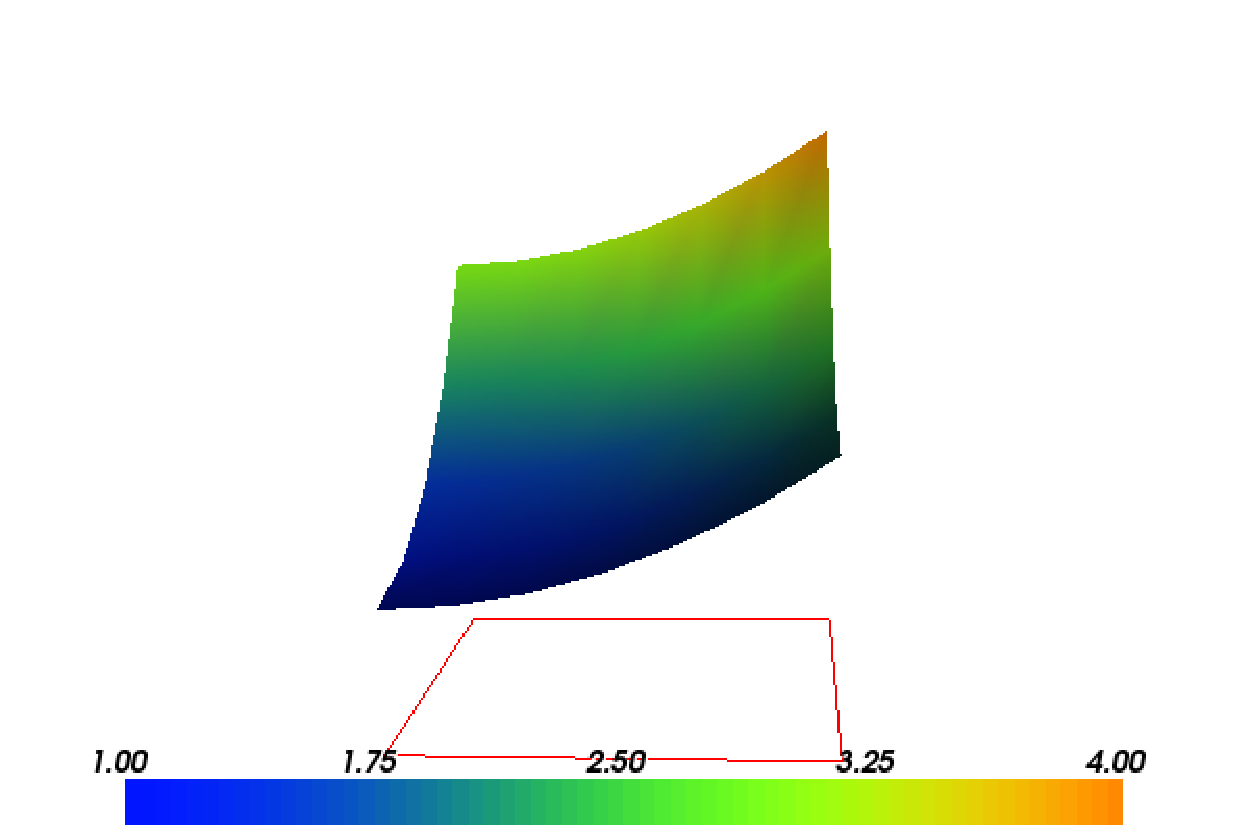
\includegraphics[width=\largefig]{chapters/langtangen/pdf/ex1_u.pdf}
  \caption{Plot of the solution in the first \fenics{} example.
    (A bounding box around the mesh is added by pressing \emp{o} in the plot
    window, and the mouse buttons are then used to rotate and move the
    plot, see Section~\ref{langtangen:quickviz}.)}
  \label{langtangen:poisson:2D:fig:ex1:u}
\end{figure}

\begin{figure}
\vspace*{12pt}
\bwfig
  \centering
  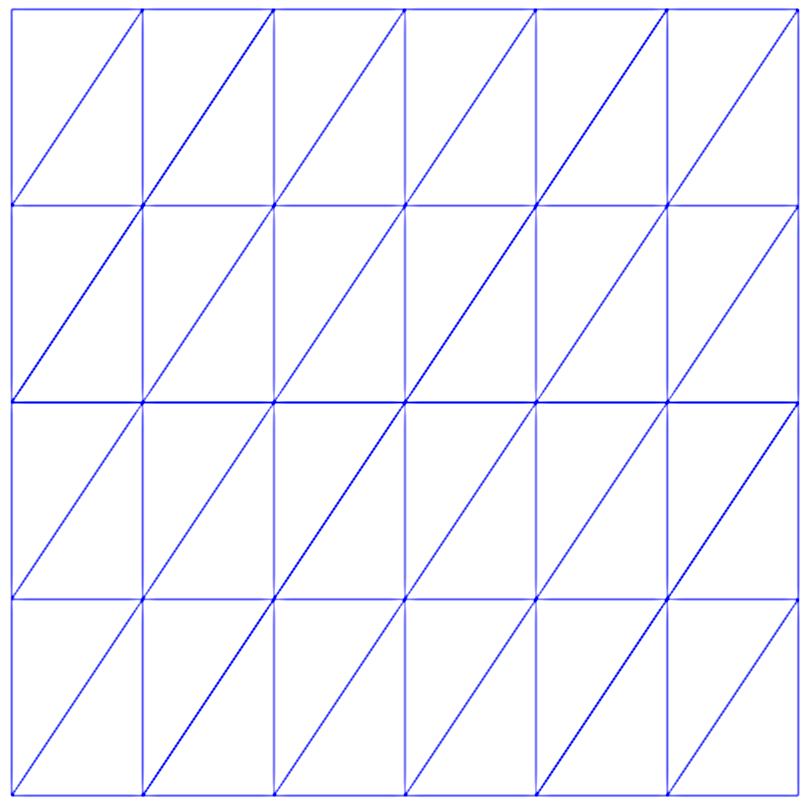
\includegraphics[width=\smallfig]{chapters/langtangen/png/ex1_mesh.png}
  \caption{Plot of the mesh in the first \fenics{} example.}
  \label{langtangen:poisson:2D:fig:ex1:mesh}
\end{figure}

The next three sections deal with some technicalities about specifying
the solution method for linear systems (so that you can solve large
problems) and examining array data from the computed solution (so that
you can check that the program is correct).  These technicalities are
scattered around in forthcoming programs. However, the impatient reader who
is more interested in seeing the previous program being adapted to a
real physical problem, and play around with some interesting
visualizations, can safely jump to Section~\ref{langtangen:poisson:membrane}.
Information in the intermediate sections can be studied on demand.

\subsection{Controlling the solution process}
\label{langtangen:poisson1:solve:prm}

Sparse LU decomposition (Gaussian elimination)
is used by default to solve linear systems of equations in \fenics{} programs.
This is a very robust and recommended method for a few thousand
unknowns in the equation system, and may hence be the method of
choice in many 2D and smaller 3D problems. However, sparse LU
decomposition becomes slow and memory demanding in large problems.
This fact forces the use of iterative methods, which are faster
and require much less memory.

Preconditioned Krylov solvers is a type of popular iterative methods that are
easily accessible in \fenics{} programs. The Poisson equation results in
a symmetric, positive definite coefficient matrix, for which the optimal
Krylov solver is the Conjugate Gradient (CG) method. Incomplete
LU factorization (ILU) is a popular and
robust all-round preconditioner, so let us try the CG--ILU pair:
\begin{python}
solve(a == L, u, bc)
      solver_parameters={"linear_solver": "cg",
                         "preconditioner": "ilu"})
# Alternative syntax
solve(a == L, u, bc,
      solver_parameters=dict(linear_solver="cg",
                             preconditioner="ilu"))
\end{python}
Section~\ref{langtangen:app:solver:prec} lists the most
popular choices of Krylov solvers and preconditioners available in
\fenics.

\index{linear algebra backend}\index{PETSc}\index{Trilinos}\index{MTL4}\index{uBLAS}
The actual CG and ILU implementations that are brought into action depends on
the choice of linear algebra package. \fenics{} interfaces
several linear algebra packages, called \emph{linear algebra backends}
in \fenics{} terminology.
PETSc is the default choice if \dolfin{} is compiled with PETSc,
otherwise uBLAS.  Epetra (Trilinos) and MTL4 are two other
supported backends.
Which backend to apply can
be controlled by setting
\begin{python}
parameters["linear_algebra_backend"] = backendname
\end{python}
where \emp{backendname} is a string, either \emp{"PETSc"}, \emp{"uBLAS"},
\emp{"Epetra"}, or \emp{"MTL4"}.  All these backends offer high-quality
implementations of both iterative and direct solvers for linear systems
of equations.

A common platform for \fenics{} users is Ubuntu Linux.  The \fenics{}
distribution for Ubuntu contains PETSc, making this package the default
linear algebra backend.  The default solver is sparse LU decomposition
(\emp{"lu"}), and the actual software that is called\index{UMFPACK}
is then the sparse LU solver from UMFPACK (which PETSc has an
interface to).

\index{parameters}
We will normally like to control
the tolerance in the stopping criterion and the maximum number
of iterations when running an iterative method.
Such parameters can be set by accessing
the \emph{global parameter database}, which is called
\emp{parameters} and behaves as a nested dictionary. Write
\index{\emp{info}}
\begin{python}
info(parameters, True)
\end{python}
to list all parameters and their default values in the database.
The nesting of parameter sets is indicated through indentation in the
output from \emp{info}.
According to this output, the relevant parameter set is
named \emp{"krylov\_solver"}, and the parameters are set like this:
\begin{python}
prm = parameters["krylov_solver"] # short form
prm["absolute_tolerance"] = 1E-10
prm["relative_tolerance"] = 1E-6
prm["maximum_iterations"] = 1000
\end{python}
Stopping criteria for Krylov solvers usually involve the norm of
the residual, which must be smaller than the absolute tolerance
parameter and smaller than the relative tolerance parameter times
the initial residual.

To see the number of actual iterations to reach the stopping criterion,
we can insert
\begin{python}
set_log_level(PROGRESS)
# or
set_log_level(DEBUG)
\end{python}
A message with the equation system size, solver type, and number of
iterations arises from specifying the argument \emp{PROGRESS}, while
\emp{DEBUG} results in more information, including CPU time spent in
the various parts of the matrix assembly and solve process.

The complete solution process with control of the solver parameters
now contains the statements
\begin{python}
prm = parameters["krylov_solver"] # short form
prm["absolute_tolerance"] = 1E-10
prm["relative_tolerance"] = 1E-6
prm["maximum_iterations"] = 1000
set_log_level(PROGRESS)

solve(a == L, u, bc,
      solver_parameters={"linear_solver": "cg",
                         "preconditioner": "ilu"})
\end{python}
The demo program \emp{d2\_p2D.py} in the
\emp{stationary/poisson} directory incorporates the above shown control
of the linear solver and precnditioner, but
is otherwise similar to the previous \emp{d1\_p2D.py} program.

We remark that default values for the global parameter database can be
defined in an XML file, see the example file
\emp{dolfin\_parameters.xml} in the directory
\emp{stationary/poisson}.  If such a file is found in the directory
where a FEniCS program is run, this file is read and used to
initialize the \emp{parameters} object. Otherwise, the file
\emp{.config/fenics/dolfin\_parameters.xml} in the user's home directory is
read, if it exists.  The XML file can also be in gzip'ed form with the
extension \emp{.xml.gz}.

\subsection{Linear variational problem and solver objects}
\label{langtangen:poisson1:solver:problem}
\index{\emp{LinearVariationalProblem}}
\index{\emp{LinearVariationalSolver}}

The \emp{solve(a == L, u, bc)} call
is just a compact syntax alternative to a slightly more comprehensive
specification of the variational equation
and the solution of the associated linear system.
This alternative syntax is used in a lot of \fenics{} applications
and will also be used later in this tutorial, so we show it already now:
\begin{python}
u = Function(V)
problem = LinearVariationalProblem(a, L, u, bc)
solver  = LinearVariationalSolver(problem)
solver.solve()
\end{python}

Many objects have an attribute \emp{parameters} corresponding to
a parameter set in the global \emp{parameters} database,
but local to the object. Here, \emp{solver.parameters} play that
role. Setting the CG method with ILU preconditiong as solution
method and specifying solver-specific parameters can be done
like this:
\begin{python}
solver.parameters["linear_solver"] = "cg"
solver.parameters["preconditioner"] = "ilu"
cg_prm = solver.parameters["krylov_solver"] # short form
cg_prm["absolute_tolerance"] = 1E-7
cg_prm["relative_tolerance"] = 1E-4
cg_prm["maximum_iterations"] = 1000
\end{python}
Calling \emp{info(solver.parameters, True)} lists all the available
parameter sets with default values for each parameter.
Settings in the global \emp{parameters} database are
propagated to parameter sets in individual objects, with the
possibility of being overwritten as done above.

The \emp{d3\_p2D.py} program modifies the \emp{d2\_p2D.py} file
to incorporate objects for the variational problem and solver.


\subsection{Examining the discrete solution}
\label{langtangen:poisson1:verify1}

We know that, in the particular boundary-value problem of
Section~\ref{langtangen:poisson1:impl}, the computed solution $u$ should
equal the exact solution at the vertices of the cells.  An important
extension of our first program is therefore to examine the computed
values of the solution, which is the focus of the present section.

A finite element function like $u$ is expressed as a linear combination
of basis functions $\phi_j$, spanning the space $V$:
\begin{equation}
  \sum_{j=1}^N U_j \phi_j.
\label{langtangen:poisson1:ufem}
\end{equation}
By writing \emp{solve(a == L, u, bc)} in the program, a linear system
will be formed from $a$ and $L$, and this system is solved for
the $U_1,\ldots,U_N$ values. The $U_1,\ldots,U_N$ values are known
\index{degrees of freedom} as \emph{degrees of freedom} of $u$. For
Lagrange elements (and many other element types) $U_k$ is simply the value
of $u$ at the node with global number $k$.  (The nodes and cell vertices
coincide for linear Lagrange elements, while for higher-order elements
there may be additional nodes at the facets and in the interior of cells.)

Having \emp{u} represented as a \emp{Function} object, we can either
evaluate \emp{u(x)} at any vertex \emp{x} in the mesh, or we can grab
all the values $U_j$ directly by
\begin{python}
u_nodal_values = u.vector()
\end{python}
The result is a \dolfin{} \emp{Vector} object, which is basically an
encapsulation of the vector object used in the linear algebra package
that is used to solve the linear system arising from the variational
problem.  Since we program in Python it is convenient to convert
the \emp{Vector} object to a standard \emp{numpy} array for further
processing:
\begin{python}
u_array = u_nodal_values.array()
\end{python}
With \emp{numpy} arrays we can write ``MATLAB-like'' code to analyze
the data. Indexing is done with square brackets: \emp{u\_array[i]},
where the index \emp{i} always starts at \emp{0}.

Mesh information can be gathered from the \emp{mesh} object, e.g.,
\begin{itemize}
  \item \emp{mesh.coordinates()} returns the coordinates of the
  vertices as an $M\times d$ \emp{numpy} array,
  $M$ being the number of vertices in the mesh and $d$ being
  the number of space dimensions,

  \item \emp{mesh.num\_cells()} returns the number of cells (triangles)
  in the mesh,

  \item \emp{mesh.num\_vertices()} returns the number of vertices in
  the mesh (with our choice of linear Lagrange elements this equals the
  number of nodes),

  \item \emp{str(mesh)} returns a short ``pretty print'' description of
  the mesh, e.g.,
\begin{progoutput}
<Mesh of topological dimension 2 (triangles) with
16 vertices and 18 cells, ordered>
\end{progoutput}
  \noindent
  and \emp{print mesh} is actually the same as \emp{print str(mesh)}.
\end{itemize}
All mesh objects are of type \emp{Mesh} so typing the command \emp{pydoc
dolfin.Mesh}\index{pydoc} in a terminal window will give a list
of methods\footnote{A method in Python (and other
  languages supporting the class construct) is simply a function in a
  class.} that can be called through any \emp{Mesh} object. In fact,
\emp{pydoc dolfin.X} shows the documentation of any \dolfin{} name \emp{X}.

Writing out the solution on the screen can now be done by a simple loop:
\begin{python}
coor = mesh.coordinates()
if mesh.num_vertices() == len(u_array):
    for i in range(mesh.num_vertices()):
        print 'u(%8g,%8g) = %g' % (coor[i][0], coor[i][1], u_array[i])
\end{python}
The beginning of the output looks like this:
\begin{progoutput}
u(       0,       0) = 1
u(0.166667,       0) = 1.02778
u(0.333333,       0) = 1.11111
u(     0.5,       0) = 1.25
u(0.666667,       0) = 1.44444
u(0.833333,       0) = 1.69444
u(       1,       0) = 2
\end{progoutput}
\noindent
For Lagrange elements of degree higher than one, the vertices do not
correspond to all the nodal points and the \emp{if}-test fails.

For verification purposes we want to compare the values of the
computed \emp{u} at the nodes (given by \emp{u\_array}) with the exact
solution \emp{u0} evaluated at the nodes.  The difference between the
computed and exact solution should be less than a small tolerance at
all the nodes. The \emp{Expression} object \emp{u0} can be evaluated
at any point \emp{x} by calling \emp{u0(x)}. Specifically,
\emp{u0(coor[i])} returns the value of \emp{u0} at the vertex or node
with global number \emp{i}.
Alternatively, we can make a finite element field \emp{u\_e}, representing
the exact solution, whose values at the nodes are given by the
\emp{u0} function. With mathematics, $u_{\rm e} = \sum_{j=1}^N  E_j\phi_j$, where
$E_j=u_0(x_j,y_j)$, $(x_j,y_j)$ being the coordinates of node number $j$.
This process is known as interpolation.\index{interpolation}
\fenics{} has a function for performing the operation:
\begin{python}
u_e = interpolate(u0, V)
\end{python}
The maximum error can now be computed as
\begin{python}
u_e_array = u_e.vector().array()
print "Max error:", numpy.abs(u_e_array - u_array).max()
\end{python}
The value of the error should be at the level of the machine precision
($10^{-16}$).

To demonstrate the use of point evaluations of \emp{Function} objects,
we write out the computed \emp{u} at the center point of the domain and
compare it with the exact solution:
\begin{python}
center = (0.5, 0.5)
print "numerical u at the center point:",  u(center)
print "exact     u at the center point:", u0(center)
\end{python}
Trying a $3\times 3$ mesh, the output from the previous snippet becomes
\begin{progoutput}
numerical u at the center point: [ 1.83333333]
exact     u at the center point: [ 1.75]
\end{progoutput}
\noindent
The discrepancy is due to the fact that the center point is not a node in
this particular mesh, but a point in the interior of a cell, and \emp{u}
varies linearly over the cell while \emp{u0} is a quadratic function.

We have seen how to extract the nodal values in a \emp{numpy} array.
If desired, we can adjust the nodal values too. Say we want to normalize
the solution such that the maximum value is 1. Then we must divide all $U_j$
values by $\max\{U_1,\ldots,U_N\}$. The following snippet performs the task:
\begin{python}
max_u = u_array.max()
u_array /= max_u
u.vector()[:] = u_array
u.vector().set_local(u_array)  # alternative
print u.vector().array()
\end{python}
That is, we manipulate \emp{u\_array} as desired, and then we insert
this array into \emp{u}'s \emp{Vector} object.  The \emp{/=} operator
implies an in-place modification of the object on the left-hand side:
all elements of the \emp{u\_array} are divided by the value \emp{max\_u}.
Alternatively, one could write \emp{u\_array =
  u\_array/max\_u}, which implies creating a new array on the
right-hand side and assigning this array to the name \emp{u\_array}.

A call like \emp{u.vector().array()} returns a copy of the data in
\emp{u.vector()}. One must therefore never perform assignments like
\emp{u.vector.array()[:] = ...}, but instead extract the
\emp{numpy} array (that is, a copy), manipulate it, and insert
it back with \emp{u.vector()[:] = } or \emp{u.set\_local(...)}.

All the code in this subsection can be found in the file
\emp{d4\_p2D.py} in the \emp{stationary/poisson} directory.
%We have commented out the \emp{plot} and \emp{interactive} calls in
%this version of the program, but if you want plotting to happen, make
%sure that \emp{interactive} is called at the very end of the program.

\subsection{Solving a real physical problem}
\label{langtangen:poisson:membrane}

Perhaps you are not particularly amazed by viewing the simple surface
of $u$ in the test problem from
Section~\ref{langtangen:poisson1:impl}.  However, solving a real
physical problem with a more interesting and amazing solution on the
screen is only a matter of specifying a more exciting domain, boundary
condition, and/or right-hand side $f$.

One possible physical problem regards the deflection $D(x,y)$ of an
elastic circular membrane with radius $R$, subject to a localized
perpendicular pressure force, modeled as a Gaussian function.
The appropriate PDE model is
\begin{equation}
-T\Delta D = p(x,y)\quad\hbox{in }\Omega = \{ (x,y)\,|\, x^2+y^2\leqslant R\},
\end{equation}
with
\begin{equation}
p(x,y) = \frac{A}{2\pi\sigma}\exp{\left(
- \frac{1}{2}\left( \frac{x-x_0}{\sigma}\right)^2
- \frac{1}{2}\left( \frac{y-y_0}{\sigma}\right)^2
\right)}.
\end{equation}
Here, $T$ is the tension in the membrane (constant), $p$ is the
external pressure load, $A$ the amplitude of the pressure, $(x_0,y_0)$
the localization of the Gaussian pressure function, and $\sigma$ the
``width'' of this function. The boundary of the membrane has no
deflection, implying $D=0$ as boundary condition.

For scaling and verification it is convenient to simplify the problem
to find an analytical solution. In the limit $\sigma\rightarrow\infty$,
$p\rightarrow A/(2\pi\sigma)$, which allows us to integrate an axi--symmetric
version of the equation in the radial coordinate $r\in [0,R]$ and
obtain $D(r)=(r^2-R^2)A/(8\pi\sigma T)$. This result gives
a rought estimate of the characteristic size of the deflection:
$|D(0)|=AR^2/(8\pi\sigma T)$, which can be used to scale the deflection.
With $R$ as characteristic length scale, we can derive the equivalent
dimensionless problem on the unit circle,
\begin{equation}
\label{langtangen:poisson1:membrane:scaled:eq}
-\Delta w = f,
\end{equation}
with $w=0$ on the boundary and with
\begin{equation}
\label{langtangen:poisson1:membrane:scaled:eq:rhs}
f(x,y) = 4\exp{\left(
- \frac{1}{2}\left( \frac{Rx-x_0}{\sigma}\right)^2
- \frac{1}{2}\left( \frac{Ry-y_0}{\sigma}\right)^2
\right)}.
\end{equation}
For notational convenience we have dropped introducing
new symbols for the scaled
coordinates in \eqref{langtangen:poisson1:membrane:scaled:eq:rhs}.
Now $D$ is related to $w$ through $D = AR^2w/(8\pi\sigma T)$.

Let us list the modifications of the
\emp{d1\_p2D.py} program that are needed to solve this membrane problem:
\begin{enumerate}
  \item Initialize $T$, $A$, $R$, $x_0$, $y_0$, and $\sigma$,

  \item create a mesh over the unit circle,

  \item make an expression object for the scaled pressure function $f$,

  \item define the \emp{a} and \emp{L} formulas in the variational
  problem for $w$ and compute the solution,

  \item plot the mesh, $w$, and $f$,

  \item write out the maximum real deflection $D$,
\end{enumerate}

\noindent
Some suitable values of $T$, $A$, $R$, $x_0$, $y_0$, and $\sigma$ are
\begin{python}
T = 10.0  # tension
A = 1.0   # pressure amplitude
R = 0.3   # radius of domain
theta = 0.2
x0 = 0.6*R*cos(theta)
y0 = 0.6*R*sin(theta)
sigma = 0.025
\end{python}

A mesh over the unit circle can be created by
\begin{python}
mesh = UnitCircle(n)
\end{python}
where \emp{n} is the typical number of elements in the radial direction.

The function $f$ is represented by an \emp{Expression} object. There
are many physical parameters in the formula for $f$ that enter
the expression string and these parameters must have their values set
by keyword arguments:
\index{expression!with parameters}
\begin{python}
f = Expression("4*exp(-0.5*(pow((R*x[0] - x0)/sigma, 2)) "\
               "     - 0.5*(pow((R*x[1] - y0)/sigma, 2)))",
               R=R, x0=x0, y0=y0, sigma=sigma)
\end{python}
The coordinates in \emp{Expression} objects \emph{must} be a vector
with indices 0, 1, and 2, and with the name \emp{x}. Otherwise
we are free to introduce names of parameters as long as these are
given default values by keyword arguments. All the parameters
initialized by keyword arguments can at any time have their
values modified. For example, we may set
\begin{python}
f.sigma = 50
f.x0 = 0.3
\end{python}

\index{interpolation}
It would be of interest to visualize $f$ along with $w$ so that we can
examine the pressure force and its response.  We must then transform
the formula (\emp{Expression}) to a finite element function
(\emp{Function}).  The most natural approach is to construct a finite
element function whose degrees of freedom (values at the nodes in this case)
are calculated from $f$. That is, we interpolate $f$ (see
Section~\ref{langtangen:poisson1:verify1}):
\begin{python}
f = interpolate(f, V)
\end{python}
Calling \emp{plot(f)} will produce a plot of $f$. Note that the assignment
to \emp{f} destroys the previous \emp{Expression} object \emp{f}, so if
it is of interest to still have access to this object another name must be used
for the \emp{Function} object returned by \emp{interpolate}.

We need some evidence that the program works, and to this end we may
use the analytical solution listed above for the case
$\sigma\rightarrow\infty$. In scaled coordinates the solution reads
\[ w_{\rm}(x,y) = 1-x^2-y^2 .\]
Practical values for an infinite $\sigma$
may be 50 or larger, and in such cases the program will report the
maximum deviation between the computed $w$ and the (approximate) exact
$w_{\rm e}$.

Note that the variational formulation remains the same as in the
program from Section~\ref{langtangen:poisson1:impl}, except that $u$ is
replaced by $w$ and $u_0=0$.
The final program is found in the file \emp{membrane1.py}, located
in the \emp{stationary/poisson} directory, and also listed below.
We have inserted capabilities for iterative solution methods and
hence large meshes (Section~\ref{langtangen:poisson1:solve:prm}),
used objects for the variational problem and solver
(Section~\ref{langtangen:poisson1:solver:problem}), and made numerical
comparison of the numerical and (approximate) analytical solution
(Section~\ref{langtangen:poisson1:verify1}).
\begin{python}
from dolfin import *

# Set pressure function:
T = 10.0  # tension
A = 1.0   # pressure amplitude
R = 0.3   # radius of domain
theta = 0.2
x0 = 0.6*R*cos(theta)
y0 = 0.6*R*sin(theta)
sigma = 0.025
#sigma = 50  # large value for verification
n = 40   # approx no of elements in radial direction
mesh = UnitCircle(n)
V = FunctionSpace(mesh, "Lagrange", 1)

# Define boundary condition w=0
def boundary(x, on_boundary):
    return on_boundary

bc = DirichletBC(V, Constant(0.0), boundary)

# Define variational problem
w = TrialFunction(V)
v = TestFunction(V)
a = inner(nabla_grad(w), nabla_grad(v))*dx
f = Expression("4*exp(-0.5*(pow((R*x[0] - x0)/sigma, 2)) "\
               "     - 0.5*(pow((R*x[1] - y0)/sigma, 2)))",
               R=R, x0=x0, y0=y0, sigma=sigma)
L = f*v*dx

# Compute solution
w = Function(V)
problem = LinearVariationalProblem(a, L, w, bc)
solver  = LinearVariationalSolver(problem)
solver.parameters["linear_solver"] = "cg"
solver.parameters["preconditioner"] = "ilu"
solver.solve()

# Plot scaled solution, mesh and pressure
plot(mesh, title="Mesh over scaled domain")
plot(w, title="Scaled deflection")
f = interpolate(f, V)
plot(f, title="Scaled pressure")

# Find maximum real deflection
max_w = w.vector().array().max()
max_D = A*max_w/(8*pi*sigma*T)
print "Maximum real deflection is", max_D

# Verification for "flat" pressure (large sigma)
if sigma >= 50:
    w_exact = Expression("1 - x[0]*x[0] - x[1]*x[1]")
    w_e = interpolate(w_exact, V)
    dev = numpy.abs(w_e.vector().array() - w.vector().array()).max()
    print 'sigma=%g: max deviation=%e' % dev

# Should be at the end
interactive()
\end{python}

Choosing a small width $\sigma$ (say 0.01) and a location $(x_0,y_0)$
toward the circular boundary (say $(0.6R\cos\theta, 0.6R\sin\theta)$
for any $\theta\in [0,2\pi]$), may produce an exciting visual
comparison of $w$ and $f$ that demonstrates the very smoothed elastic
response to a peak force (or mathematically, the smoothing properties
of the inverse of the Laplace operator).  One needs to experiment with
the mesh resolution to get a smooth visual representation of~$f$.  You
are strongly encouraged to play around with the plots and different
mesh resolutions.

\subsection{Quick visualization with VTK}
\label{langtangen:quickviz}
\index{visualization}\index{Viper}\index{VTK}

As we go along with examples it is fun to play around with \emp{plot}
commands and visualize what is computed. This section explains some
useful visualization features.

The \emp{plot(u)} command launches a \fenics{} component called Viper,
which applies the VTK package to visualize finite element functions.
Viper is not a full-fledged, easy-to-use front-end to VTK (like
Mayavi2, ParaView, or VisIt), but rather a thin layer on top of VTK's
Python interface, allowing us to quickly visualize a \dolfin{}
function or mesh, or data in plain Numerical Python arrays, within a
Python program.  Viper is ideal for debugging, teaching, and initial
scientific investigations.  The visualization can be interactive, or
you can steer and automate it through program statements.  More
advanced and professional visualizations are usually better done with
advanced tools like MayaVi2, ParaView, or VisIt.

We have made a program \emp{membrane1v.py} for the membrane deflection
problem in Section~\ref{langtangen:poisson:membrane} and added various
demonstrations of Viper capabilities. You are encouraged to play around
with \emp{membrane1v.py} and modify the code as you read about various
features.

The \emp{plot} function can take additional arguments, such as a title
of the plot, or a specification of a wireframe plot (elevated mesh)
instead of a colored surface plot:\index{\emp{plot}}
\begin{python}
plot(mesh, title="Finite element mesh")
plot(w, wireframe=True, title="solution")
\end{python}

The three mouse buttons can be used to rotate, translate, and zoom
the surface.  Pressing \emp{h} in the plot window makes a printout of
several key bindings that are available in such windows. For example,
pressing \emp{m} in the mesh plot window dumps the plot of the mesh to an
Encapsulated PostScript (\emp{.eps}) file, while pressing \emp{i} saves
the plot in PNG format.  All file names are automatically generated as
\emp{simulationX.eps}, where \emp{X} is a counter \emp{0000}, \emp{0001},
\emp{0002}, etc., being increased every time a new plot file in that
format is generated (the extension of PNG files is \emp{.png} instead
of \emp{.eps}).  Pressing \emp{o} adds a red outline of a bounding box
around the domain.

One can alternatively control the visualization from the program code
directly. This is done through a \emp{Viper} object returned from the
\emp{plot} command. Let us grab this object and use it to 1) tilt the
camera $-65$ degrees in the latitude direction, 2) add $x$ and $y$ axes, 3)
change the default name of the plot files, 4) change the color scale, and 5)
write the plot to a PNG and an EPS file. Here is the code:
\begin{python}
viz_w = plot(w,
            wireframe=False,
            title="Scaled membrane deflection",
            rescale=False,
            axes=True,              # include axes
            basename="deflection",  # default plotfile name
            )

viz_w.elevate(-65) # tilt camera -65 degrees (latitude dir)
viz_w.set_min_max(0, 0.5*max_w)  # color scale
viz_w.update(w)    # bring settings above into action
viz_w.write_png("deflection.png")
viz_w.write_ps("deflection", format="eps")
\end{python}
The \emp{format} argument in the latter line can also take the values
\emp{"ps"} for a standard PostScript file and \emp{"pdf"} for a PDF file.
Note the necessity of the \emp{viz\_w.update(w)} call -- without it we
will not see the effects of tilting the camera and changing the color
scale. Figure~\ref{langtangen:poisson:2D:fig1} shows the resulting
scalar surface.
\begin{figure}
  \centering
  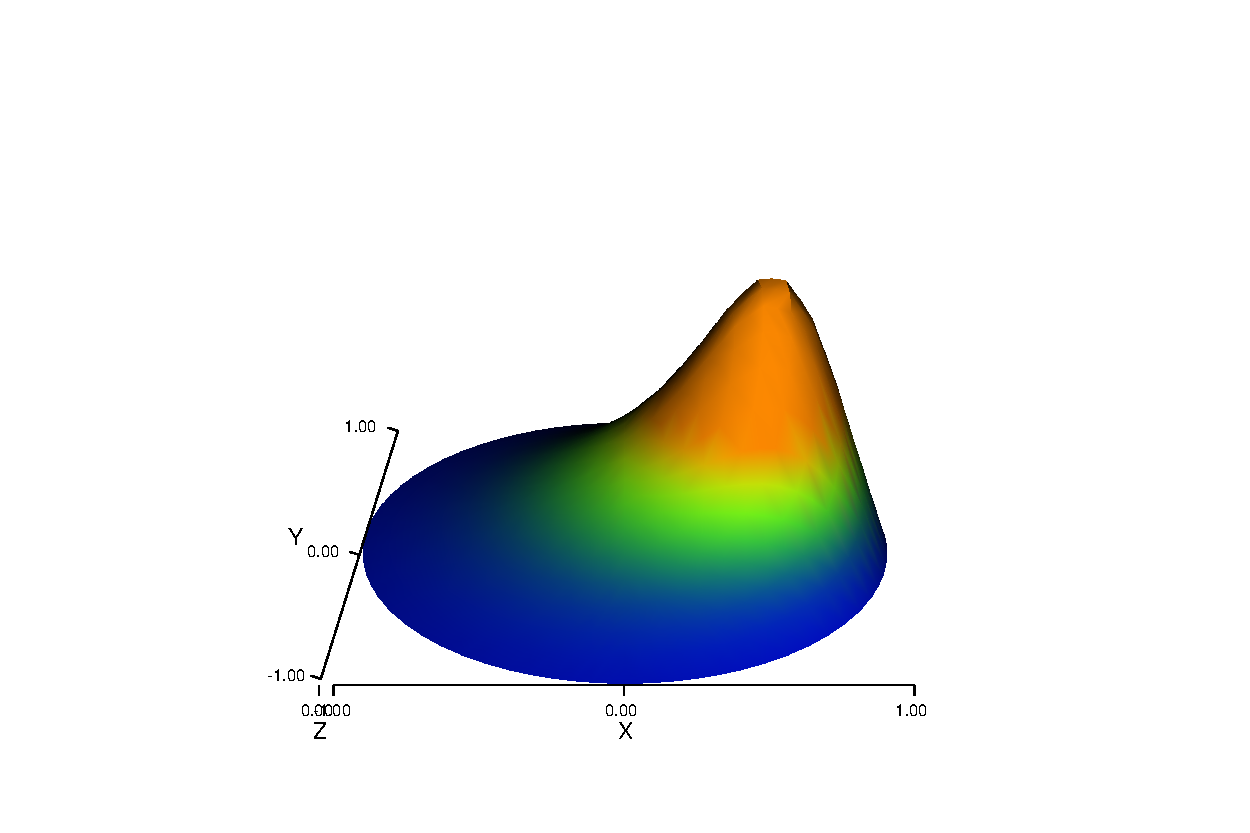
\includegraphics[width=\largefig]{chapters/langtangen/pdf/membrane_waxis.pdf}
  \caption{Plot of the deflection of a membrane.}
  \label{langtangen:poisson:2D:fig1}
\end{figure}

\subsection{Computing derivatives}
\label{langtangen:poisson:gradu}

In Poisson and many other problems the gradient of the solution is of
interest. The computation is in principle simple: since $u = \sum_{j=1}^N
U_j \phi_j$, we have that
\begin{equation}
  \nabla u = \sum_{j=1}^N U_j \nabla \phi_j.
\end{equation}
Given the solution variable \emp{u} in the program,
its gradient is obtained by \emp{grad(u)} or \emp{nabla\_grad(u)}.
However, the gradient of a piecewise continuous finite
element scalar field is a discontinuous vector field since the $\phi_j$
has discontinuous derivatives at the boundaries of the cells. For example,
using Lagrange elements of degree 1, $u$ is linear over each cell, and
the numerical $\nabla u$ becomes a piecewise constant vector field. On
the contrary, the exact gradient is continuous.  For visualization
and data analysis purposes we often want the computed gradient to be a
continuous vector field. Typically, we want each component of $\nabla
u$ to be represented in the same way as $u$ itself. To this end,
we can project the components of $\nabla u$ onto the same function
space as we used for $u$.  This means that we solve $w = \nabla u$
approximately by a finite element method. This process is known as
\emph{projection}. \index{projection}
Looking at the component $\partial
u/\partial x$ of the gradient, we project the (discrete) derivative
$\sum_jU_j{\partial \phi_j/\partial x}$ onto a function space
with basis $\phi_1,\phi_2,\ldots$ such that the derivative in
this space is expressed by the standard sum $\sum_j\bar U_j \phi_j$,
for suitable (new) coefficients $\bar U_j$.

The variational problem for $w$ reads: find $w\in V^{(\mbox{g})}$ such that
\begin{equation}
  a(w, v) = L(v)\quad\foralls v\in \hat{V}^{(\mbox{g})},
\end{equation}
where
\begin{align}
  a(w, v) &= \int_\Omega w\cdot v\dx,
\\
  L(v) &= \int_\Omega \nabla u\cdot v\dx.
\end{align}
The function spaces $V^{(\mbox{g})}$ and $\hat{V}^{(\mbox{g})}$ (with
the superscript g denoting ``gradient'') are vector versions of the
function space for $u$, with boundary conditions removed (if $V$ is
the space we used for $u$, with no restrictions on boundary values, $
V^{(\mbox{g})} = \hat{V}^{(\mbox{g})} = [V]^d$, where $d$ is the
number of space dimensions).  For example, if we used piecewise linear
functions on the mesh to approximate $u$, the variational problem for
$w$ corresponds to approximating each component field of $w$ by
piecewise linear functions.

The variational problem for the vector field $w$, called \emp{grad\_u}
in the code, is easy to solve in \fenics:
\begin{python}
V_g = VectorFunctionSpace(mesh, "Lagrange", 1)
w = TrialFunction(V_g)
v = TestFunction(V_g)

a = inner(w, v)*dx
L = inner(grad(u), v)*dx
grad_u = Function(V_g)
solve(a == L, grad_u)

plot(grad_u, title="grad(u)")
\end{python}
The boundary condition argument to \emp{solve} is dropped since there are
no essential boundary conditions in this problem.
The new thing is basically that we work with a
\emp{VectorFunctionSpace}, since the unknown is now a vector
field, instead of the \emp{FunctionSpace} object for scalar fields.
Figure~\ref{langtangen:poisson:2D:fig:ex1:gradu} shows an example of how Viper
can visualize such a vector field.

\begin{figure}
  \centering
  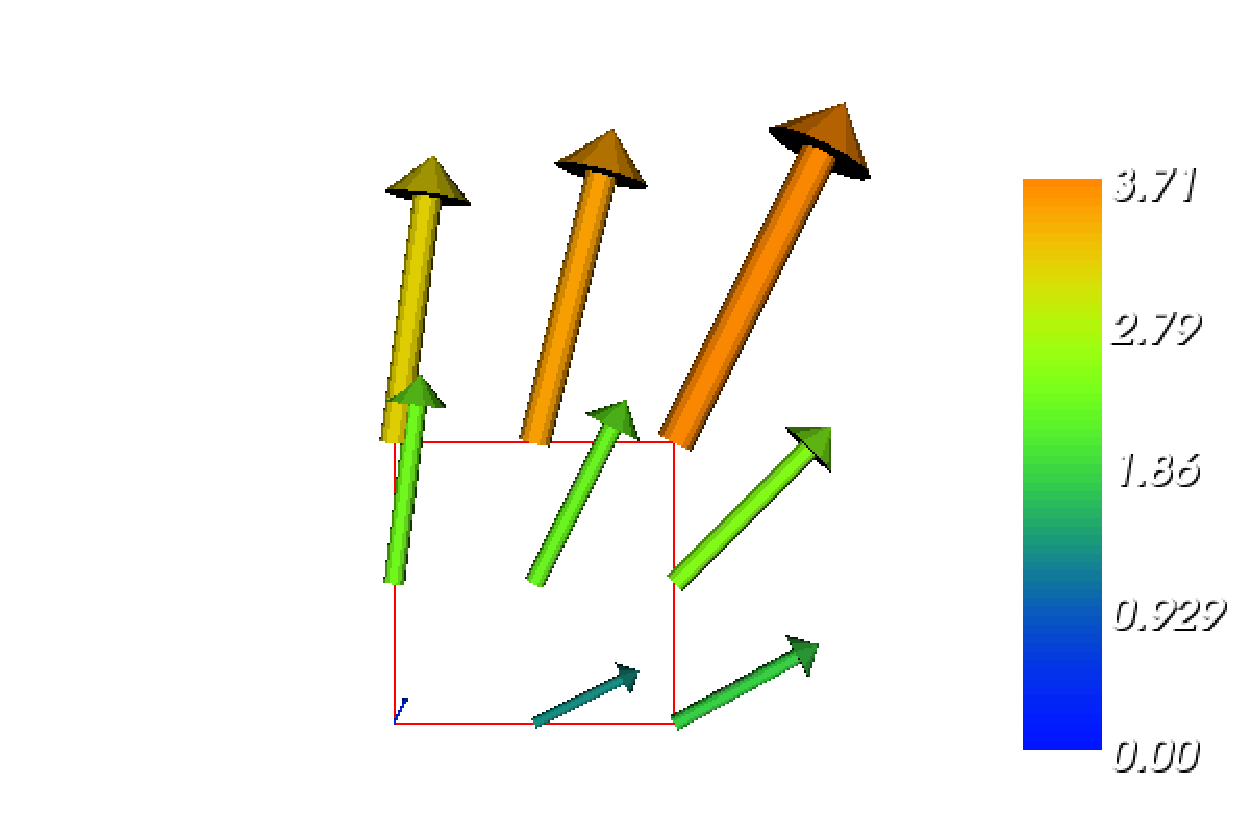
\includegraphics[width=\largefig]{chapters/langtangen/pdf/ex1_gradu.pdf}
  \caption{Example of visualizing the vector field
    $\nabla u$ by arrows at the nodes.}
  \label{langtangen:poisson:2D:fig:ex1:gradu}
\end{figure}

The scalar component fields of the gradient can be extracted as separate
fields and, e.g., visualized:
\begin{python}
grad_u_x, grad_u_y = grad_u.split(deepcopy=True)  # extract components
plot(grad_u_x, title="x-component of grad(u)")
plot(grad_u_y, title="y-component of grad(u)")
\end{python}
The \emp{deepcopy=True} argument signifies a \emph{deep copy}, which
is a general term in computer science implying that a copy of the data
is returned. (The opposite, \emp{deepcopy=False}, means a \emph{shallow
copy}, where the returned objects are just pointers to the original data.)

The \emp{grad\_u\_x} and \emp{grad\_u\_y} variables behave as \emp{Function}
objects. In particular, we can extract the underlying arrays of nodal
values by
\begin{python}
grad_u_x_array = grad_u_x.vector().array()
grad_u_y_array = grad_u_y.vector().array()
\end{python}
The degrees of freedom of the \emp{grad\_u} vector field can also be
reached by \index{degrees of freedom array!vector field}
\begin{python}
grad_u_array = grad_u.vector().array()
\end{python}
but this is a flat \emp{numpy} array where the degrees of freedom for
the $x$ component of the gradient is stored in the first part, then the
degrees of freedom of the $y$ component, and so on.

The program \emp{d5\_p2D.py} extends the code \emp{d4\_p2D.py}
from Section~\ref{langtangen:poisson1:verify1} with computations
and visualizations of the gradient.  Examining the arrays
\emp{grad\_u\_x\_array} and \emp{grad\_u\_y\_array}, or looking at the
plots of \emp{grad\_u\_x} and \emp{grad\_u\_y}, quickly reveals that the
computed \emp{grad\_u} field does not equal the exact gradient $(2x,
4y)$ in this particular test problem where $u=1+x^2+2y^2$.  There are
inaccuracies at the boundaries, arising from the approximation problem for
$w$. Increasing the mesh resolution shows, however, that the components
of the gradient vary linearly as $2x$ and $4y$ in the interior of
the mesh (as soon as we are one element away from the boundary). See
Section~\ref{langtangen:quickviz} for illustrations of this phenomenon.

Projecting some function onto some space is a very common
operation in finite element programs. The manual steps in this process
have therefore been collected in a utility function \emp{project(q, W)},
which returns the projection of some \emp{Function} or \emp{Expression} object
named \emp{q} onto the \emp{FunctionSpace} or \emp{VectorFunctionSpace}
named \emp{W}.
Specifically, the previous code for
projecting each component of \emp{grad(u)} onto
the same sapce that we use for \emp{u}, can now be done by
a one--line call:
\index{project}\index{projection}
\begin{python}
grad_u = project(grad(u), VectorFunctionSpace(mesh, "Lagrange", 1))
\end{python}
The applications of projection are many, including turning discontinuous
gradient fields into continuous ones, comparing higher- and lower-order
function approximations, and transforming a higher-order finite element
solution down to a piecewise linear field, which is required by many
visualization packages.

\subsection{A variable-coefficient Poisson problem}
\label{langtangen:possion:2D:varcoeff}
\index{Poisson's equation!variable coefficient}

Suppose we have a variable coefficient $p(x,y)$ in the Laplace operator,
as in the boundary-value problem
\begin{equation} \label{langtangen:poisson:2D:varcoeff}
  \begin{split}
    - \nabla\cdot \left\lbrack
p(x,y)\nabla u(x,y)\right\rbrack &= f(x,y) \quad \mbox{in } \Omega,
    \\
    u(x,y) &= u_0(x,y) \quad \mbox{on}\  \partial\Omega.
  \end{split}
\end{equation}
We shall quickly demonstrate that this simple extension of our model
problem only requires an equally simple extension of the \fenics{} program.

Let us continue to use our favorite solution $u(x,y)=1+x^2+2y^2$ and
then prescribe $p(x,y)=x+y$. It follows that $u_0(x,y) = 1 + x^2 + 2y^2$
and $f(x,y)=-8x-10y$.

What are the modifications we need to do in the \emp{d4\_p2D.py}
program from Section~\ref{langtangen:poisson1:verify1}?
\begin{enumerate}
  \item \emp{f} must be an \emp{Expression} since it is no longer
  a constant,

  \item a new \emp{Expression} \emp{p} must be defined for the variable
  coefficient,

  \item the variational problem is slightly changed.
\end{enumerate}
First we address the modified variational problem. Multiplying the PDE
in \eqref{langtangen:poisson:2D:varcoeff} and integrating by parts now
results in
%
\begin{equation}
  \int_\Omega p\nabla u\cdot\nabla v\dx -
  \int_{\partial\Omega} p \frac{\partial u}{\partial n}v\ds = \int_\Omega
  fv\dx.
\end{equation}
%
The function spaces for $u$ and $v$ are the same as in
Section~\ref{langtangen:poisson1:varform}, implying that the boundary
integral vanishes since $v=0$ on $\partial\Omega$ where we have Dirichlet
conditions.  The weak form $a(u,v)=L(v)$ then has
\begin{align}
  a(u,v) &= \int_\Omega p\nabla u\cdot\nabla v\dx,
\\
  L(v) &= \int_\Omega fv\dx.
\end{align}
In the code from Section~\ref{langtangen:poisson1:impl} we must replace
\begin{python}
a = inner(nabla_grad(u), nabla_grad(v))*dx
\end{python}
by
\begin{python}
a = p*inner(nabla_grad(u), nabla_grad(v))*dx
\end{python}
The definitions of \emp{p} and \emp{f} read
\begin{python}
p = Expression("x[0] + x[1]")
f = Expression("-8*x[0] - 10*x[1]")
\end{python}
No additional modifications are necessary. The complete code can be
found in in the file\break \emp{vcp2D.py} (variable-coefficient Poisson problem in 2D). You can run it and confirm
that it recovers the exact $u$ at the nodes.

The flux $-p\nabla u$ may be of particular interest in
variable-coefficient Poisson problems as it often has an interesting
physical significance. As explained in
Section~\ref{langtangen:poisson:gradu}, we normally want the piecewise
discontinuous flux or gradient to be approximated by a continuous
vector field, using the same elements as used for the numerical
solution $u$. The approximation now consists of solving $w = -p\nabla
u$ by a finite element method: find $w\in V^{(\mbox{g})}$ such that
\begin{equation}
a(w, v) = L(v)\quad\foralls v\in \hat{V}^{(\mbox{g})},
\end{equation}
where
\begin{align}
a(w, v) &= \int_\Omega w\cdot v\dx,
\\
L(v) &= \int_\Omega (-p \nabla u)\cdot v\dx.
\end{align}
This problem is identical to the one in Section~\ref{langtangen:poisson:gradu},
except that $p$ enters the integral in $L$.

The relevant Python statements for computing the flux field take the form
\begin{python}
V_g = VectorFunctionSpace(mesh, "Lagrange", 1)
w = TrialFunction(V_g)
v = TestFunction(V_g)

a = inner(w, v)*dx
L = inner(-p*grad(u), v)*dx
flux = Function(V_g)
solve(a == L, flux)
\end{python}
The following call to \emp{project} is equivalent to the above statements:
\begin{python}
flux = project(-p*nabla_grad(u),
               VectorFunctionSpace(mesh, "Lagrange", 1))
\end{python}

Plotting the flux vector field is naturally as easy as plotting
the gradient in Section~\ref{langtangen:poisson:gradu}:
\begin{python}
plot(flux, title="flux field")

flux_x, flux_y = flux.split(deepcopy=True)  # extract components
plot(flux_x, title="x-component of flux (-p*grad(u))")
plot(flux_y, title="y-component of flux (-p*grad(u))")
\end{python}

For data analysis of the nodal values of the flux field we can
grab the underlying \emp{numpy} arrays:
\begin{python}
flux_x_array = flux_x.vector().array()
flux_y_array = flux_y.vector().array()
\end{python}

The program \emp{vcp2D.py} contains in
addition some plots, including a curve plot comparing
\emp{flux\_x} and the exact counterpart along
the line $y=1/2$.  The associated programming details related to this
visualization are explained in Section~\ref{langtangen:structviz}.

\subsection{Computing functionals}
\label{langtangen:poisson1:functionals}
\index{functional}

After the solution $u$ of a PDE is computed, we occasionally want to compute
functionals of $u$, for example,
\begin{equation}
  \frac{1}{2} ||\nabla u||^2 \equiv \frac{1}{2}\int_\Omega \nabla u\cdot \nabla u\dx,
\label{langtangen:poisson1:functionals:energy}
\end{equation}
which often reflects some energy quantity.  Another frequently
occurring functional is the error
\begin{equation}
  ||u_{\rm e}-u|| = \left(\int_\Omega (u_{\rm e}-u)^2\dx\right)^{1/2},
\label{langtangen:poisson1:functionals:error}
\end{equation}
where $u_{\rm e}$ is the exact solution. The error
is of particular interest when studying convergence properties.
Sometimes the interest concerns the flux out of a part $\Gamma$ of the
boundary $\partial\Omega$,
\begin{equation}
  F = -\int_\Gamma p\nabla u\cdot  \ds,
\label{langtangen:poisson1:functionals:flux}
\end{equation}
where $n$ is an outward unit normal
at $\Gamma$ and $p$ is a coefficient (see the problem in
Section~\ref{langtangen:possion:2D:varcoeff} for a specific example).
All these functionals are easy to compute with \fenics, and this section
describes how it can be done.

\paragraph{Energy functional.}\index{energy functional}
The integrand of the energy functional
\eqref{langtangen:poisson1:functionals:energy} is described in the UFL
language in the same manner as we describe weak forms:
\begin{python}
energy = 0.5*inner(grad(u), grad(u))*dx
E = assemble(energy)
\end{python}
The \emp{assemble} call performs the integration.  It is possible to
restrict the integration to subdomains, or parts of the boundary,
by using a mesh function to mark the subdomains (this technique will be
explained
in Section~\ref{langtangen:poisson:mat:neumann}).  The program
\emp{membrane2.py} carries out the computation of the elastic energy
\begin{equation}
   \frac{1}{2}||T\nabla D||^2 = \frac{1}{2}\left(\frac{AR}{8\pi\sigma}\right)^2
    ||\nabla w||^2
\end{equation}
in the membrane problem from Section~\ref{langtangen:poisson:membrane}.

\paragraph{Convergence estimation.}\index{error functional}
To illustrate error computations and convergence of finite element
solutions, we modify the \emp{d5\_p2D.py} program from
Section~\ref{langtangen:poisson:gradu} and specify a more complicated
solution,
\begin{equation}
   u(x,y) = \sin(\omega\pi x)\sin(\omega\pi y)
\end{equation}
on the unit square.  This choice implies $f(x,y)=2\omega^2\pi^2 u(x,y)$.
With $\omega$ restricted to an integer it follows that $u_0=0$. We must
define the appropriate boundary conditions, the exact solution, and the
$f$ function in the code:
\begin{python}
def boundary(x, on_boundary):
    return on_boundary

bc = DirichletBC(V, Constant(0.0), boundary)

omega = 1.0
u_e = Expression("sin(omega*pi*x[0])*sin(omega*pi*x[1])",
                 omega=omega)

f = 2*pi**2*omega**2*u_e
\end{python}

The computation of \eqref{langtangen:poisson1:functionals:error} can be
done by
\begin{python}
error = (u - u_e)**2*dx
E = sqrt(assemble(error))
\end{python}
Here, \emp{u\_e} will be interpolated onto the function
space \emp{V}. This implies that the exact solution used in the integral will
vary linearly over the cells, and not as a sine function, if \emp{V}
corresponds to linear Lagrange elements.  This situation
may yield a smaller error
\emp{u - u\_e} than what is actually true.

More accurate representation of the exact solution is easily achieved by
interpolating the formula onto a space defined by higher-order elements,
say of third degree:
\begin{python}
Ve = FunctionSpace(mesh, "Lagrange", degree=3)
u_e_Ve = interpolate(u_e, Ve)
error = (u - u_e_Ve)**2*dx
E = sqrt(assemble(error))
\end{python}
To achieve complete mathematical
control of which function space the computations are carried out in,
we can explicitly interpolate \emp{u} too:
\begin{python}
u_Ve = interpolate(u, Ve)
error = (u_Ve - u_e_Ve)**2*dx
\end{python}

The square in the expression for \emp{error} will be expanded and lead
to a lot of terms that almost cancel when the error is small, with the
potential of introducing significant round-off errors.  The function
\emp{errornorm} is available for avoiding this effect by first
interpolating \emp{u} and \emp{u\_e} to a space with higher-order
elements, then subtracting the degrees of freedom, and then performing
the integration of the error field. The usage is simple:
\begin{python}
E = errornorm(u_e, u, normtype="L2", degree=3)
\end{python}
It is illustrative to look at the short implementation of \emp{errornorm}:
\begin{python}
def errornorm(u_e, u, Ve):
    u_Ve = interpolate(u, Ve)
    u_e_Ve = interpolate(u_e, Ve)
    e_Ve = Function(Ve)
    # Subtract degrees of freedom for the error field
    e_Ve.vector()[:] = u_e_Ve.vector().array() - \
                       u_Ve.vector().array()
    error = e_Ve**2*dx
    return sqrt(assemble(error))
\end{python}
The \emp{errornorm} procedure turns out to be identical to computing
the expression \emp{(u\_e - u)**2*dx} directly in the present test case.

Sometimes it is of interest to compute the error of the gradient field:
$||\nabla (u-u_{\rm e})||$ (often referred to as the $H^1$ seminorm of the
error).  Given the error field \emp{e\_Ve} above, we simply write
\begin{python}
H1seminorm = sqrt(assemble(inner(grad(e_Ve), grad(e_Ve))*dx))
\end{python}

Finally, we remove all \emp{plot} calls and printouts of $u$ values in
the original program, and collect the computations in a function:
\begin{python}
def compute(nx, ny, degree):
    mesh = UnitSquare(nx, ny)
    V = FunctionSpace(mesh, "Lagrange", degree=degree)
    ...
    Ve = FunctionSpace(mesh, "Lagrange", degree=5)
    E = errornorm(u_e, u, Ve)
    return E
\end{python}

Calling \emp{compute} for finer and finer meshes enables us to study
the convergence rate. Define the element size $h=1/n$, where $n$ is the
number of divisions in $x$ and $y$ direction (\emp{nx=ny} in the code). We
perform experiments with $h_0>h_1>h_2\cdots$ and compute the corresponding
errors $E_0, E_1, E_3$ and so forth.  Assuming $E_i=Ch_i^r$ for unknown
constants $C$ and $r$, we can compare two consecutive experiments,
$E_i=Ch_i^r$ and $E_{i-1}=Ch_{i-1}^r$, and solve for $r$:
\begin{equation}
  r = \frac{\ln(E_i/E_{i-1})}{\ln (h_i/h_{i-1})}.
\end{equation}
The $r$ values should approach the expected convergence rate
\emp{degree+1} as $i$ increases.

The procedure above can easily be turned into Python code:
\begin{python}
import sys
degree = int(sys.argv[1])  # read degree as 1st command-line arg
h = []  # element sizes
E = []  # errors
for nx in [4, 8, 16, 32, 64, 128, 264]:
    h.append(1.0/nx)
    E.append(compute(nx, nx, degree))

# Convergence rates
from math import log as ln  # (log is a dolfin name too)
for i in range(1, len(E)):
    r = ln(E[i]/E[i-1])/ln(h[i]/h[i-1])
    print "h=%10.2E r=%.2f" % (h[i], r)
\end{python}
The resulting program has the name \emp{d6\_p2D.py} and computes
error norms in various ways. Running this program for elements of first
degree and $\omega=1$ yields the output
\begin{progoutput}
h=1.25E-01 E=3.25E-02 r=1.83
h=6.25E-02 E=8.37E-03 r=1.96
h=3.12E-02 E=2.11E-03 r=1.99
h=1.56E-02 E=5.29E-04 r=2.00
h=7.81E-03 E=1.32E-04 r=2.00
h=3.79E-03 E=3.11E-05 r=2.00
\end{progoutput}
\noindent
That is, we approach the expected second-order convergence of linear
Lagrange elements as the meshes become sufficiently fine.

Running the program for second-degree elements results in the expected
value $r=3$,
\begin{progoutput}
h=1.25E-01 E=5.66E-04 r=3.09
h=6.25E-02 E=6.93E-05 r=3.03
h=3.12E-02 E=8.62E-06 r=3.01
h=1.56E-02 E=1.08E-06 r=3.00
h=7.81E-03 E=1.34E-07 r=3.00
h=3.79E-03 E=1.53E-08 r=3.00
\end{progoutput}
\noindent
However, using \emp{(u - u\_e)**2} for the error computation, which
implies interpolating \emp{u\_e} onto the same space as \emp{u},
results in $r=4$ (!). This is an example where it is important to
interpolate \emp{u\_e} to a higher-order space (polynomials of
degree 3 are sufficient here) to avoid computing a too optimistic
convergence rate.
%Looking at the error in the degrees of freedom
%(\emp{u.vector().array()}) reveals a convergence rate of $r=4$ for
%second-degree elements. For elements of polynomial degree 3 all the rates
%are $r=4$, regardless of whether we choose a ``fine'' space \emp{Ve}
%with polynomials of degree 3 or~5.

Running the program for third-degree elements results in the expected
value~$r=4$:
\begin{progoutput}
h=1.25E-01 r=4.09
h=6.25E-02 r=4.03
h=3.12E-02 r=4.01
h=1.56E-02 r=4.00
h=7.81E-03 r=4.00
\end{progoutput}
\noindent
Checking convergence rates is the next best method for verifying
PDE codes (the best being exact recovery of a solution as in
Section~\ref{langtangen:poisson1:verify1} and many other places in
this tutorial).


\paragraph{Flux functionals.}\index{flux functional}
To compute flux integrals like
\eqref{langtangen:poisson1:functionals:flux} we need to define the
$n$ vector, referred to as \emph{facet normal} in
\fenics. If $\Gamma$ is the complete boundary we can perform the flux
computation by
\begin{python}
n = FacetNormal(mesh)
flux = -p*dot(nabla_grad(u), n)*ds
total_flux = assemble(flux)
\end{python}
Although \emp{nabla\_grad(u)} and \emp{grad(u)} are interchangeable
in the above expression when \emp{u} is a scalar function, we have
chosen to write \emp{nabla\_grad(u)} because this is
the right expression if we generalize the underlying equation
to a vector Laplace/Poisson PDE. With \emp{grad(u)} we must in that
case write \emp{dot(n, grad(u))}.

It is possible to restrict the integration to a part of the boundary
using a mesh function to mark the relevant part, as explained in
Section~\ref{langtangen:poisson:mat:neumann}. Assuming that the part
corresponds to subdomain number \emp{i}, the relevant form for the flux
is \emp{-p*dot(nabla\_grad(u), n)*ds(i)}.

\subsection{Visualization of structured mesh data}
\label{langtangen:structviz}
\index{structured mesh}
\index{visualization!of structured mesh}

When finite element computations are done on a structured rectangular
mesh, maybe with uniform partitioning, VTK-based tools for completely
unstructured 2D/3D meshes are not required.  Instead we can use
visualization and data analysis tools for \emph{structured
  data}. Such data typically appear in finite difference simulations and
image analysis.  Analysis and visualization of structured data are faster
and easier than doing the same with data on unstructured meshes, and
the collection of tools to choose among is much larger.  We shall
demonstrate the potential of such tools and how they allow for
tailored and flexible visualization and data analysis.

A necessary first step is to transform our
\emp{mesh} object to an object representing
a rectangle with equally-shaped \emph{rectangular} cells.  The Python
package \emp{scitools} has this type of
structure, called a
\emp{UniformBoxGrid}. The second step is to
transform the one-dimensional array of nodal values to a
two-dimensional array holding the values at the corners of the cells
in the structured grid. In such grids, we want to access a value by
its $i$ and $j$ indices, $i$ counting cells in the $x$ direction, and
$j$ counting cells in the $y$ direction.  This transformation is in
principle straightforward, yet it frequently leads to obscure indexing
errors. The \emp{BoxField} object in
\emp{scitools} takes conveniently care of
the details of the transformation.  With a
\emp{BoxField} defined on a
\emp{UniformBoxGrid} it is very easy to call
up more standard plotting packages to visualize the solution along
lines in the domain or as 2D contours or lifted surfaces.

Let us go back to the \emp{vcp2D.py} code from
Section~\ref{langtangen:possion:2D:varcoeff} and map \emp{u} onto a
\emp{BoxField} object:
\begin{python}
import scitools.BoxField
u2 = u if u.ufl_element().degree() == 1 else \
     interpolate(u, FunctionSpace(mesh, "Lagrange", 1))
u_box = scitools.BoxField.dolfin_function2BoxField(
        u2, mesh, (nx,ny), uniform_mesh=True)
\end{python}
The function
\emp{dolfin\_function2BoxField} can only work
with finite element fields with \emph{linear} (degree 1) elements, so
for higher-degree elements we here simply interpolate the solution
onto a mesh with linear elements. We could also
interpolate/project onto a finer
mesh in the higher-degree case.  Such transformations to linear finite
element fields are very often needed when calling up plotting packages
or data analysis tools.  The
\emp{u.ufl\_element()} method returns an object
holding the element type, and this object has a method
\emp{degree()} for returning the element
degree as an integer.  The parameters
\emp{nx} and
\emp{ny} are the number of divisions in each
space direction that were used when calling
\emp{UnitSquare} to make the
\emp{mesh} object.  The result
\emp{u\_box} is a
\emp{BoxField} object that supports ``finite
difference'' indexing and an underlying grid suitable for
\emp{numpy} operations on 2D data.  Also 1D
and 3D meshes (with linear elements) can be turned
into \emp{BoxField} objects.

The ability to access a finite element field in the way one can access
a finite difference-type of field is handy in many occasions,
including visualization and data analysis.  Here is an example of
writing out the coordinates and the field value at a grid point with
indices \emp{i} and
\emp{j} (going from 0 to
\emp{nx} and
\emp{ny}, respectively, from lower left to
upper right corner):
\begin{python}
X = 0; Y = 1; Z = 0  # convenient indices

i = nx; j = ny   # upper right corner
print "u(%g,%g)=%g" % (u_box.grid.coor[X][i],
                       u_box.grid.coor[Y][j],
                       u_box.values[i,j])
\end{python}
For instance,
the $x$ coordinates are reached by \emp{u\_box.grid.coor[X]}.
The \emp{grid} attribute is an instance of class \emp{UniformBoxGrid}.

Many plotting programs can be used to visualize the data in
\emp{u\_box}. Matplotlib is now a very popular
plotting program in the Python world and could be used to make contour
plots of \emp{u\_box}. However, other programs
like Gnuplot, VTK, and MATLAB have better support for surface
plots at the time of this writing.
Our choice in this tutorial is to use the Python package
\emp{scitools.easyviz}, which offers a
uniform MATLAB-like syntax as interface to various plotting packages
such as Gnuplot, matplotlib, VTK, OpenDX, MATLAB, and others. With
\emp{scitools.easyviz} we write one set of
statements, close to what one would do in MATLAB or Octave, and then
it is easy to switch between different plotting programs, at a later
stage, through a command-line option, a line in a configuration file,
or an import statement in the program.

A contour plot is made by the following \emp{scitools.easyviz} command:
\index{contour plot}
\begin{python}
import scitools.easyviz as ev
ev.contour(u_box.grid.coorv[X], u_box.grid.coorv[Y], u_box.values,
           5, clabels="on")
ev.title("Contour plot of u")
ev.savefig("u_contours.eps")

# or more compact syntax:
ev.contour(u_box.grid.coorv[X], u_box.grid.coorv[Y], u_box.values,
           5, clabels="on",
           savefig="u_contours.eps", title="Contour plot of u")
\end{python}
The resulting plot can be viewed in
Figure~\ref{langtangen:poisson:2D:fig2}a.  The
\emp{contour} function needs arrays with the
$x$ and $y$ coordinates expanded to 2D arrays (in the same way as
demanded when making vectorized \emp{numpy}
calculations of arithmetic expressions over all grid points).  The
correctly expanded arrays are stored in
\emp{grid.coorv}.  The above call to
\emp{contour} creates 5 equally spaced
contour lines, and with \emp{clabels="on"}
the contour values can be seen in the plot.

Other functions for visualizing 2D scalar fields are \emp{surf} and
\emp{mesh} as known from MATLAB:
\begin{python}
import scitools.easyviz as ev
ev.figure()
ev.surf(u_box.grid.coorv[X], u_box.grid.coorv[Y], u_box.values,
        shading="interp", colorbar="on",
        title="surf plot of u", savefig="u_surf.eps")

ev.figure()
ev.mesh(u_box.grid.coorv[X], u_box.grid.coorv[Y], u_box.values,
        title="mesh plot of u", savefig="u_mesh.eps")
\end{python}
Figure~\ref{langtangen:poisson:2D:fig3} exemplifies the surfaces
arising from the two plotting commands above.  You can type
\emp{pydoc scitools.easyviz} in a terminal
window to get a full tutorial.
Note that \emp{scitools.easyviz} offers function names like
\emp{plot} and \emp{mesh}, which clash with \emp{plot} from \emp{dolfin}
and the \emp{mesh} variable in our programs. Therefore, we recommend the
\emp{ev} prefix.

A handy feature of \emp{BoxField} is the
ability to give a start point in the grid and a direction, and then
extract the field and corresponding coordinates along the nearest grid
line. In 3D fields one can also extract data in a plane.  Say we want
to plot $u$ along the line $y=1/2$ in the grid. The grid points,
\emp{x}, and the $u$ values along this line,
\emp{uval}, are extracted by
\begin{python}
start = (0, 0.5)
x, uval, y_fixed, snapped = u_box.gridline(start, direction=X)
\end{python}
The variable \emp{snapped} is true if the line had to be snapped onto a
grid line and in that case \emp{y\_fixed} holds the snapped
(altered) $y$ value.
Plotting $u$ versus the $x$ coordinate along this line, using
\emp{scitools.easyviz}, is now a matter of
\begin{python}
ev.figure()  # new plot window
ev.plot(x, uval, "r-")  # "r--: red solid line
ev.title("Solution")
ev.legend("finite element solution")

# or more compactly:
ev.plot(x, uval, "r-", title="Solution",
        legend="finite element solution")
\end{python}

A more exciting plot compares the projected numerical flux in
$x$ direction along the
line $y=1/2$ with the exact flux:
\begin{python}
ev.figure()
flux2_x = flux_x if flux_x.ufl_element().degree() == 1 else \
          interpolate(flux_x, FunctionSpace(mesh, "Lagrange", 1))
flux_x_box = scitools.BoxField.dolfin_function2BoxField(
          flux2_x, mesh, (nx,ny), uniform_mesh=True)
x, fluxval, y_fixed, snapped = \
          flux_x_box.gridline(start, direction=X)
y = y_fixed
flux_x_exact = -(x + y)*2*x
ev.plot(x, fluxval, "r-",
        x, flux_x_exact, "b-",
        legend=("numerical (projected) flux", "exact flux"),
        title="Flux in x-direction (at y=%g)" % y_fixed,
        savefig="flux.eps")
\end{python}
As seen from Figure~\ref{langtangen:poisson:2D:fig2}b, the numerical flux
is accurate except in the elements closest to the boundaries.

The visualization constructions shown above and used to generate the
figures are found in the program \emp{vcp2D.py} in the
\emp{stationary/poisson} directory.


\begin{figure}
  \centering
  \subfloat[]{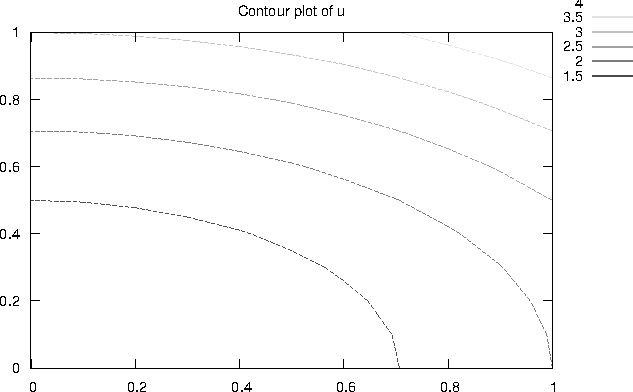
\includegraphics[width=\twofigs]{chapters/langtangen/pdf/Poisson2D_Dvc_contour1.pdf}}
  \subfloat[]{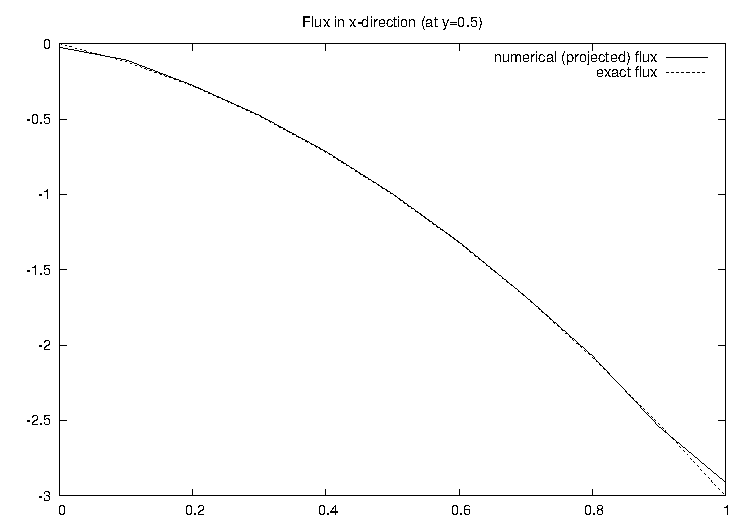
\includegraphics[width=\twofigs]{chapters/langtangen/pdf/Poisson2D_Dvc_flux_x.pdf}}
  \caption{Examples of plots created by transforming the finite
    element field to a field on a uniform, structured 2D grid: (a)
    contour plot of the solution; (b) curve plot of the exact flux
    $-p\partial u/\partial x$ against the corresponding projected
    numerical flux.}
  \label{langtangen:poisson:2D:fig2}
\end{figure}

\begin{figure}
  \centering
  \subfloat[]{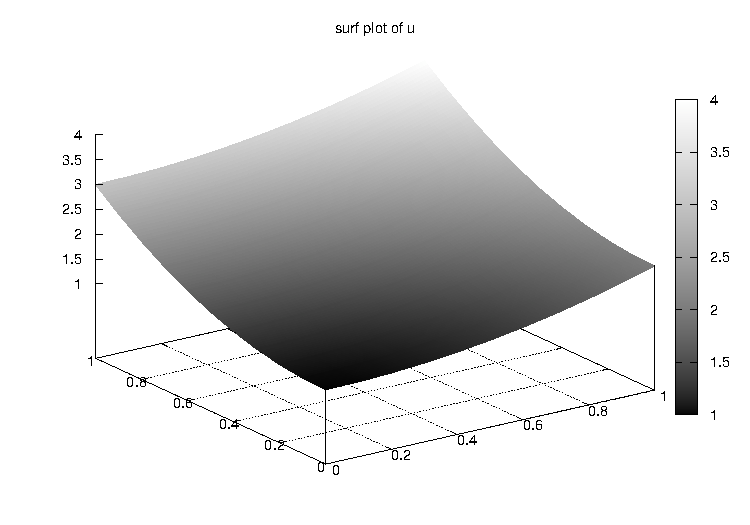
\includegraphics[width=\twofigs]{chapters/langtangen/pdf/Poisson2D_Dvc_surf1.pdf}}
  \subfloat[]{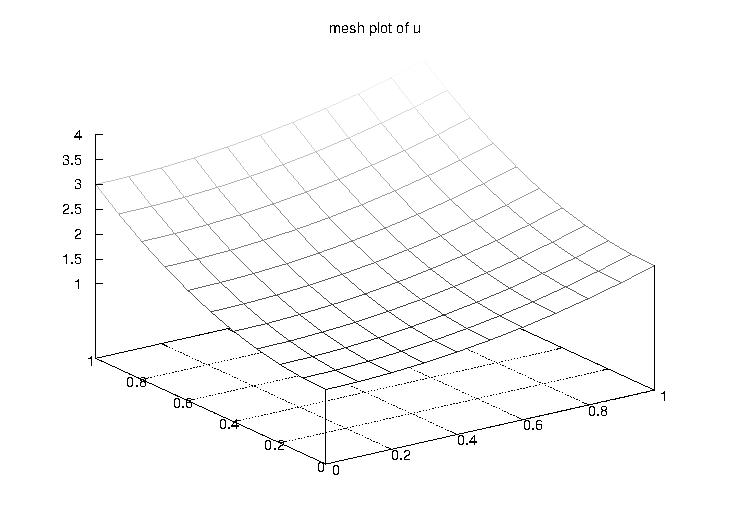
\includegraphics[width=\twofigs]{chapters/langtangen/pdf/Poisson2D_Dvc_mesh1.pdf}}
  \caption{Examples of plots created by transforming the finite
    element field to a field on a uniform, structured 2D grid: (a) a
    surface plot of the solution; (b) lifted mesh plot of the
  solution.}
  \label{langtangen:poisson:2D:fig3}
\end{figure}

It should be easy with the information above to transform a finite element
field over a uniform rectangular or box-shaped mesh to the corresponding
\emp{BoxField} object and perform MATLAB-style
visualizations of the whole field or
the field over planes or along lines through the domain.
By the transformation to a regular grid we have some more flexibility
than what Viper offers. However, we must remark that
comprehensive tools like
VisIt, MayaVi2, or ParaView also have the possibility for plotting fields
along lines and extracting planes in 3D geometries, though usually with
less degree of control compared to Gnuplot, MATLAB, and matplotlib.


\subsection{Combining Dirichlet and Neumann conditions}
\label{langtangen:poisson1:DN}

Let us make a slight extension of our two-dimensional Poisson problem
from Section~\ref{langtangen:poisson1:bvp} and add a Neumann boundary
condition. The domain is still the unit square, but now we set the
Dirichlet condition $u=u_0$ at the left and right sides, $x=0$ and $x=1$,
while the Neumann condition
%%
\begin{equation}
 - \frac{\partial u}{\partial n} = g
\end{equation}
%%
is applied to the remaining sides $y=0$ and $y=1$.  The Neumann condition
is also known as a \emph{natural boundary condition} (in contrast to an
essential boundary condition).  \index{boundary condition!Neumann}

Let $\Gamma_{\mathrm{D}}$ and $\Gamma_{\mathrm{N}}$ denote the parts of $\partial\Omega$ where
the Dirichlet and Neumann conditions apply, respectively.  The complete
boundary-value problem can be written as
\begin{align}
  -\Delta u &= f \mbox{ in } \Omega,
\\
  u &= u_0 \mbox{ on } \Gamma_{\mathrm{D}},
\\
  -\frac{\partial u}{\partial n} &= g \mbox{ on } \Gamma_{\mathrm{N}}.
\end{align}
Again we choose $u=1+x^2 + 2y^2$ as the exact solution and adjust $f$,
$g$, and $u_0$ accordingly:
\begin{align}
f &= -6,
\\
g &= \left\lbrace\begin{array}{ll}
-4, & y=1\\
0,  & y=0
\end{array}\right.
\\
u_0 &= 1 + x^2 + 2y^2.
\end{align}
For ease of programming we may introduce a $g$ function defined over
the whole of $\Omega$ such that $g$ takes on the right values at $y=0$
and $y=1$. One possible extension is
\begin{equation}
   g(x,y) = -4y.
\end{equation}

The first task is to derive the variational problem. This time we cannot
omit the boundary term arising from the integration by parts, because $v$
is only zero on $\Gamma_{\mathrm{D}}$. We have
\begin{equation}
 -\int_\Omega (\Delta u)v \dx
= \int_\Omega\nabla u\cdot\nabla v\dx
  - \int_{\partial\Omega} \frac{\partial u}{\partial n}v\ds,
\end{equation}
and since $v=0$ on $\Gamma_{\mathrm{D}}$,
\begin{equation}
- \int_{\partial\Omega} \frac{\partial u}{\partial n}v\ds
=
- \int_{\Gamma_{\mathrm{N}}} \frac{\partial u}{\partial n}v\ds
= \int_{\Gamma_{\mathrm{N}}}gv\ds,
\end{equation}
by applying the boundary condition on $\Gamma_{\mathrm{N}}$.  The resulting weak
form reads
\begin{equation}
\int_{\Omega} \nabla u \cdot \nabla v \dx +
\int_{\Gamma_{\mathrm{N}}} gv\ds
= \int_{\Omega} fv \dx.
\label{langtangen:poisson:2D:DN:weak}
\end{equation}
Expressing \eqref{langtangen:poisson:2D:DN:weak} in the standard notation
$a(u,v)=L(v)$ is straightforward with
\begin{align}
  a(u, v) &= \int_{\Omega} \nabla u \cdot \nabla v \dx,
  \label{langtangen:poisson2:vard:a}
\\
  L(v) &= \int_{\Omega} fv \dx - \int_{\Gamma_{\mathrm{N}}} gv\ds.
  \label{langtangen:poisson2:vard:L}
\end{align}

How does the Neumann condition impact the implementation?  The code
in the file \emp{d4\_p2D.py} in the directory
\emp{stationary/poisson} remains almost the same.  Only two
adjustments are necessary:
\begin{enumerate}
  \item The function describing the boundary where Dirichlet conditions
  apply must be modified.

  \item The new boundary term must be added to the expression in \emp{L}.
\end{enumerate}
Step 1 can be coded as
\begin{python}
def Dirichlet_boundary(x, on_boundary):
    if on_boundary:
        if x[0] == 0 or x[0] == 1:
            return True
        else:
            return False
    else:
        return False
\end{python}
A more compact implementation reads
\begin{python}
def Dirichlet_boundary(x, on_boundary):
    return on_boundary and (x[0] == 0 or x[0] == 1)
\end{python}
As pointed out already in Section~\ref{langtangen:poisson1:impl}, testing
for an exact match of real numbers is not good programming practice so
we introduce a tolerance in the test:
\begin{python}
def Dirichlet_boundary(x, on_boundary):
    tol = 1E-14   # tolerance for coordinate comparisons
    return on_boundary and \
           (abs(x[0]) < tol or abs(x[0] - 1) < tol)
\end{python}

The second adjustment of our program concerns the definition of \emp{L},
where we have to add a boundary integral and a definition of the $g$
function to be integrated:
\begin{python}
g = Expression("-4*x[1]")
L = f*v*dx - g*v*ds
\end{python}
The \emp{ds} variable implies a boundary integral, while \emp{dx}
implies an integral over the domain $\Omega$.  No more modifications
are necessary.

The file \emp{dn1\_p2D.py} in the \emp{stationary/poisson} directory
implements this problem. Running the program verifies the implementation:
$u$ equals the exact solution at all the nodes,
regardless of how many elements we use.


\subsection{Multiple Dirichlet conditions}
\label{langtangen:poisson:multiple:Dirichlet}

The PDE problem from the previous section applies a function $u_0(x,y)$
for setting Dirichlet conditions at two parts of the boundary.
Having a single function to set multiple Dirichlet conditions is seldom
possible. The more general case is to have $m$ functions for setting
Dirichlet conditions on $m$ parts of the boundary. The purpose of this
section is to explain how such multiple conditions are treated in \fenics{}
programs.

Let us return to the case from Section~\ref{langtangen:poisson1:DN}
and define two separate functions for the two Dirichlet conditions:
\begin{align}
  - \Delta u &= -6 \mbox{ in } \Omega,
\\
  u &= u_L \mbox{ on } \Gamma_0,
\\
  u &= u_R \mbox{ on } \Gamma_1,
\\
  - \frac{\partial u}{\partial n} &= g \mbox{ on } \Gamma_{\mathrm{N}}.
\end{align}
Here, $\Gamma_0$ is the boundary $x=0$, while $\Gamma_1$ corresponds to
the boundary $x=1$.  We have that $u_L = 1 + 2y^2$, $u_R = 2 + 2y^2$,
and $g=-4y$.  For the left boundary $\Gamma_0$ we define the usual
triple of a function for the boundary value, a function for defining
the boundary of interest, and a \emp{DirichletBC} object:
\begin{python}
u_L = Expression("1 + 2*x[1]*x[1]")

def left_boundary(x, on_boundary):
    tol = 1E-14   # tolerance for coordinate comparisons
    return on_boundary and abs(x[0]) < tol

Gamma_0 = DirichletBC(V, u_L, left_boundary)
\end{python}

For the boundary $x=1$ we define a similar code:
\begin{python}
u_R = Expression("2 + 2*x[1]*x[1]")

def right_boundary(x, on_boundary):
    tol = 1E-14   # tolerance for coordinate comparisons
    return on_boundary and abs(x[0] - 1) < tol

Gamma_1 = DirichletBC(V, u_R, right_boundary)
\end{python}
The various essential conditions are then collected in a list
and used in the solution process:
\begin{python}
bcs = [Gamma_0, Gamma_1]
...
solve(a == L, u, bcs)
# or
problem = LinearVariationalProblem(a, L, u, bcs)
solver  = LinearVariationalSolver(problem)
solver.solve()
\end{python}

If the $u$ values are constant at a part of the boundary, we may use a
simple \emp{Constant} object instead of an \emp{Expression} object.

The file \emp{dn2\_p2D.py} contains a complete program which
demonstrates the constructions above.  An extended example with multiple
Neumann conditions would have been quite natural now, but this requires
marking various parts of the boundary using the mesh function concept
and is therefore left to Section~\ref{langtangen:poisson:mat:neumann}.

\subsection{A linear algebra formulation}
\label{langtangen:poisson1:linalg}

Given $a(u,v)=L(v)$, the discrete solution $u$ is computed by
inserting $u=\sum_{j=1}^N U_j \phi_j$ into $a(u,v)$ and demanding
$a(u,v)=L(v)$ to be fulfilled for $N$ test functions
$\hat\phi_1,\ldots,\hat\phi_N$. This implies
\begin{equation}
 \sum_{j=1}^N a(\phi_j,\hat\phi_i) U_j = L(\hat\phi_i),\quad i=1,\ldots,N,
\end{equation}
which is nothing but a linear system,
\begin{equation}
  AU = b,
\end{equation}
where the entries in $A$ and $b$ are given by
\begin{equation}
\begin{split}
  A_{ij} &= a(\phi_j, \hat{\phi}_i), \\
  b_i &= L(\hat\phi_i).
\end{split}
\end{equation}

The examples so far have specified the left- and right-hand side
of the variational formulation and then asked \fenics{} to
assemble the linear system and solve it.
An alternative to is explicitly call functions for assembling the
coefficient matrix $A$ and the right-side vector $b$, and then solve
the linear system $AU=b$ with respect to the $U$ vector.
Instead of \emp{solve(a == L, u, b)} we now write\index{\emp{assemble}}\index{linear system}
\begin{python}
A = assemble(a)
b = assemble(L)
bc.apply(A, b)
u = Function(V)
U = u.vector()
solve(A, U, b)
\end{python}
The variables \emp{a} and \emp{L} are as before; that is, \emp{a}
refers to the bilinear form involving a \emp{TrialFunction} object
(say \emp{u}) and a \emp{TestFunction} object (\emp{v}), and \emp{L}
involves a \emp{TestFunction} object (\emp{v}). From \emp{a} and \emp{L},
the \emp{assemble} function can compute the matrix elements $A_{i,j}$
and the vector elements~$b_i$.

The matrix $A$ and vector $b$ are first assembled without
incorporating essential (Dirichlet) boundary conditions. Thereafter,
the \emp{bc.apply(A, b)} call performs the necessary modifications to
the linear system.
When we have multiple Dirichlet conditions stored in a list \emp{bcs},
as explained in Section~\ref{langtangen:poisson:multiple:Dirichlet},
we must apply each condition in \emp{bcs} to the system:
\begin{python}
# bcs is a list of DirichletBC objects
for bc in bcs:
    bc.apply(A, b)
\end{python}

There is an alternative function \emp{assemble\_system} that can
assemble the system and take boundary conditions into account in one call:
\index{\emp{assemble\_system}}
\begin{python}
A, b = assemble_system(a, L, bcs)
\end{python}
The \emp{assemble\_system} function incorporates the boundary conditions
in the element matrices and vectors, prior to assembly.
The conditions are also incorporated in a symmetric way to preserve
eventual symmetry of the coefficient matrix.
%That is, for each degree of freedom
%that is known, the corresponding row and column is zeroed out and 1 is
%placed on the main diagonal, and the right-hand side \emp{b} is modified
%by subtracting the column in \emp{A} times the value of the degree of
%freedom, and then the corresponding entry in \emp{b} is replaced by the
%known value of the degree of freedom.
With \emp{bc.apply(A,b)}
the matrix \emp{A} is modified in an unsymmetric way.
%: The row
%is zeroed out and 1 is placed on the main diagonal, and the degree of
%freedom value is inserted in \emp{b}.)

Note that the solution \emp{u} is, as before, a \emp{Function} object.
The degrees of freedom, $U=A^{-1}b$, are filled into \emp{u}'s
\emp{Vector} object (\emp{u.vector()}) by the \emp{solve} function.

The object \emp{A} is of type \emp{Matrix}, while \emp{b} and
\emp{u.vector()} are of type \emp{Vector}. We may convert the matrix and
vector data to \emp{numpy} arrays by calling the \emp{array()} method
as shown before. If you wonder how essential boundary conditions are
incorporated in the linear system, you can print out \emp{A} and \emp{b}
before and after the \emp{bc.apply(A, b)} call:
\begin{python}
if mesh.num_cells() < 16:  # print for small meshes only
    print A.array()
    print b.array()
bc.apply(A, b)
if mesh.num_cells() < 16:
    print A.array()
    print b.array()
\end{python}

With access to the elements in \emp{A} as a \emp{numpy} array we can easily
do computations on this matrix, such as computing the eigenvalues
(using the \emp{numpy.linalg.eig} function). We can alternatively dump
\emp{A} and \emp{b} to file in MATLAB format and invoke MATLAB or Octave to
analyze the linear system.
Dumping the arrays \emp{A} and \emp{b} to MATLAB format is done by
\begin{python}
import scipy.io
scipy.io.savemat("Ab.mat", {"A": A, "b": b})
\end{python}
Writing \emp{load Ab.mat} in MATLAB or Octave will then make
the variables \emp{A} and \emp{b} available for computations.

\index{SLEPc}
Matrix processing in Python or MATLAB/Octave is only feasible for
small PDE problems since the \emp{numpy} arrays or matrices in MATLAB
file format are dense matrices. \dolfin{} also has an interface to the
eigensolver package SLEPc, which is a preferred tool for computing the
eigenvalues of large, sparse matrices of the type encountered in PDE
problems (see \emp{demo/la/eigenvalue} in the \dolfin{} source code tree for
a demo).

A complete code where the linear system $AU=b$ is explicitly assembled and
solved is found in the file \emp{dn3\_p2D.py} in the directory
\emp{stationary/poisson}. This code solves the same problem as in
\emp{dn2\_p2D.py}
(Section~\ref{langtangen:poisson:multiple:Dirichlet}).  For small
linear systems, the program writes out \emp{A} and \emp{b} before and
after incorporation of essential boundary conditions and illustrates
the difference between \emp{assemble} and \emp{assemble\_system}.
The reader is encouraged to run the code for a $2\times 1$
mesh (\emp{UnitSquare(2, 1)} and study the output of \emp{A}.

By default, \emp{solve(A, U, b)} applies sparse LU decomposition
as solver. Specification of an iterative solver and preconditioner
is done through two optional arguments:
\begin{python}
solve(A, U, b, "cg", "ilu")
\end{python}
Appropriate names of solvers and preconditioners are found in
Section~\ref{langtangen:app:solver:prec}.

To control tolerances in the stopping criterion and the maximum
number of iterations, one can explicitly form a \emp{KrylovSolver} object
and set items in its \emp{parameters} attribute
(see Section~\ref{langtangen:poisson1:solver:problem}):
\index{\emp{KrylovSolver}}
\begin{python}
solver = KrylovSolver("cg", "ilu")
solver.parameters["absolute_tolerance"] = 1E-7
solver.parameters["relative_tolerance"] = 1E-4
solver.parameters["maximum_iterations"] = 1000
u = Function(V)
U = u.vector()
set_log_level(DEBUG)
solver.solve(A, U, b)
\end{python}
The program \emp{dn4\_p2D.py} is a modification of \emp{dn3\_p2D.py}
illustrating this latter approach.

\index{random start vector (linear systems)}
The choice of start vector for the iterations in a linear solver is often
important. With the \emp{solve(A, U, b)} function the start vector
is the vector \emp{U} we feed in for the solution. A start vector
with random numbers in the interval $[-100,100]$ can be computed as
\begin{python}
n = u.vector().array().size
U = u.vector()
U[:] = numpy.random.uniform(-100, 100, n)
solver.parameters['nonzero_initial_guess'] = True
solver.solve(A, U, b)
\end{python}
Note that we must turn off the default behavior of setting the start
vector (``initial guess'') to zero.
A random start vector is included in the \emp{dn4\_p2D.py} code.

Creating the linear system explicitly in a program can have some
advantages in more advanced problem settings. For example, $A$ may
be constant throughout a time-dependent simulation, so we can avoid
recalculating $A$ at every time level and save a significant amount
of simulation time.  Sections~\ref{langtangen:timedep:diffusion1:impl}
and \ref{langtangen:timedep:diffusion1:noassemble} deal with this topic
in detail.

%In other problems, we may divide the variational
%problem and linear system into different terms, say $A=M + {\dt} K$,
%where $M$ is a matrix arising from a term like $\partial u/\partial t$,
%$K$ is a term corresponding to a Laplace operator, and ${\dt}$ is
%a time discretization parameter. When ${\dt}$ is changed in time,
%we can efficiently recompute $A = M + {\dt} K$ without
%reassembling the constant matrices $M$ and $K$. This strategy may
%speed up simulations significantly.


\subsection{Parameterizing the number of space dimensions}
\label{langtangen:poisson:nD}
\index{dimension-independent code}

\fenics{} makes it is easy to write a unified simulation code that can operate
in 1D, 2D, and 3D. We will conveniently make use of this feature in
forthcoming examples.
As an appetizer, go back to the introductory program \emp{d1\_p2D.py}
in the \emp{stationary/poisson} directory and change the mesh construction
from \emp{UnitSquare(6, 4)} to \emp{UnitCube(6, 4, 5)}. Now the domain
is the unit cube with $6\times 4\times 5$ cells.
Run the program and observe that we can solve a 3D problem without
any other modifications (!). The visualization allows you rotate to the
cube and observe the function values as colors on the boundary.

The forthcoming material introduces some convenient
technicalities such that the same program can run in 1D, 2D, or 3D
without any modifications.
Consider the simple problem
\begin{equation}
u''(x) = 2\hbox{ in }[0,1],\quad u(0)=0,\ u(1)=1,
\end{equation}
with exact solution $u(x)=x^2$. Our aim is to formulate and solve this
problem in a 2D and a 3D domain as well.
We may generalize the domain $[0,1]$ to a box of any size
in the $y$ and $z$ directions and pose homogeneous Neumann
conditions $\partial u/\partial n = 0$ at all additional boundaries
$y=\mbox{const}$ and $z=\mbox{const}$ to ensure that $u$ only varies with
$x$. For example, let us choose
a unit hypercube as domain: $\Omega = [0,1]^d$, where $d$ is the number
of space dimensions. The generalized $d$-dimensional Poisson problem
then reads
\begin{equation} \label{langtangen:poisson1:ddim}
  \begin{array}{rcll}
    \Delta u &=& 2 &\mbox{in } \Omega, \\
    u &=& 0 &\mbox{on } \Gamma_0,\\
    u &=& 1 &\mbox{on } \Gamma_1,\\
\frac{\partial u}{\partial n} &=& 0 &\mbox{on } \partial\Omega\backslash\left(
\Gamma_0\cup\Gamma_1\right),
  \end{array}
\end{equation}
where $\Gamma_0$ is the side of the hypercube where $x=0$, and
where $\Gamma_1$ is the side where $x=1$.

Implementing \eqref{langtangen:poisson1:ddim} for any $d$ is no more
complicated than solving a problem with a specific number of dimensions.
The only non-trivial part of the code is actually to define the mesh.
We use the command-line to provide user-input to the program. The first argument
can be the degree of the polynomial in the finite element basis functions.
Thereafter, we supply the
cell divisions in the various spatial directions. The number of
command-line arguments will then imply the number of space dimensions.
For example, writing \emp{3 10 3 4} on the command-line means that
we want to approximate $u$ by piecewise polynomials of degree 3,
and that the domain is a three-dimensional cube with $10\times 3\times 4$
divisions in the $x$, $y$, and $z$ directions, respectively.
Each of the $10\times 3\times 4 = 120$ boxes will
be divided into six tetrahedra.
The Python code can be quite compact:
\begin{python}
degree = int(sys.argv[1])
divisions = [int(arg) for arg in sys.argv[2:]]
d = len(divisions)
domain_type = [UnitInterval, UnitSquare, UnitCube]
mesh = domain_type[d-1](*divisions)
V = FunctionSpace(mesh, "Lagrange", degree)
\end{python}
First note that although \emp{sys.argv[2:]} holds the divisions of
the mesh, all elements of the list \emp{sys.argv[2:]} are string objects,
so we need to explicitly convert each element to an integer.
The construction \emp{domain\_type[d-1]} will pick the right name of the
object used to define the domain and generate the mesh.
Moreover, the argument \emp{*divisions}
sends each component of the list \emp{divisions} as a separate
argument. For example, in a 2D problem where \emp{divisions} has
two elements, the statement
\begin{python}
mesh = domain_type[d-1](*divisions)
\end{python}
is equivalent to
\begin{python}
mesh = UnitSquare(divisions[0], divisions[1])
\end{python}

The next part of the program is to set up the boundary conditions.
Since the Neumann conditions have $\partial u/\partial n=0$ we can
omit the boundary integral from the weak form. We then only
need to take care of Dirichlet conditions at two sides:
\begin{python}
tol = 1E-14   # tolerance for coordinate comparisons
def Dirichlet_boundary0(x, on_boundary):
    return on_boundary and abs(x[0]) < tol

def Dirichlet_boundary1(x, on_boundary):
    return on_boundary and abs(x[0] - 1) < tol

bc0 = DirichletBC(V, Constant(0), Dirichlet_boundary0)
bc1 = DirichletBC(V, Constant(1), Dirichlet_boundary1)
bcs = [bc0, bc1]
\end{python}
Note that this code is independent of the number of space dimensions.
So are the statements defining and solving
the variational problem:
\begin{python}
u = TrialFunction(V)
v = TestFunction(V)
f = Constant(-2)
a = inner(nabla_grad(u), nabla_grad(v))*dx
L = f*v*dx

u = Function(V)
solve(a == L, u, bcs)
\end{python}
The complete code is found in \emp{paD.py} (Poisson problem in any--D).

If we want to parameterize the direction in which $u$ varies, say by
the space direction number \emp{e}, we only need to replace \emp{x[0]}
in the code by \emp{x[e]}. The parameter \emp{e} could be given as a
second command-line argument.  The reader is encouraged to perform
this modification.

\section{Nonlinear problems}
\label{langtangen:poisson:nonlinear}
\label{partial differential equation!nonlinear}

Now we shall address how to solve nonlinear PDEs in \fenics. Our
sample PDE for implementation is taken as a nonlinear Poisson
equation:
\begin{equation}
-\nabla\cdot\left( q(u)\nabla u\right) = f.
\end{equation}
The coefficient $q(u)$ makes the equation nonlinear (unless $q(u)$
is constant in $u$).

To be able to easily verify our implementation, we choose the domain,
$q(u)$, $f$, and the boundary conditions such that we have a simple,
exact solution $u$. Let $\Omega$ be the unit hypercube $[0, 1]^d$ in
$d$ dimensions, $q(u)=(1+u)^m$, $f=0$, $u=0$ for $x_0=0$, $u=1$ for
$x_0=1$, and $\partial u/\partial n=0$ at all other boundaries $x_i=0$
and $x_i=1$, $i=1,\ldots,d-1$. The coordinates are now represented by
the symbols $x_0,\ldots,x_{d-1}$. The exact solution is then
\begin{equation}
u(x_0,\ldots,x_d) = \left((2^{m+1}-1)x_0 + 1\right)^{1/(m+1)} - 1.
\end{equation}

The variational formulation of our model problem reads:
find $u \in V$ such that
\begin{equation} \label{langtangen:poisson:nonlinear1}
  F(u; v) = 0 \quad \foralls v \in \hat{V},
\end{equation}
where
\begin{equation}
\label{langtangen:poisson:nonlinear2}
F(u; v) = \int_\Omega q(u)\nabla u\cdot \nabla v\dx,
\end{equation}
and
\begin{equation}
  \begin{split}
    \hat{V} &= \{v \in H^1(\Omega) : v = 0 \mbox{ on } x_0=0\mbox{ and }x_0=1\}, \\
     V      &= \{v \in H^1(\Omega) : v = 0 \mbox{ on } x_0=0\mbox{ and } v = 1\mbox{ on }x_0=1\}. \\
  \end{split}
\end{equation}
The discrete problem arises as usual by restricting $V$ and $\hat V$
to a pair of discrete spaces. As usual, we omit any subscript on
discrete spaces and simply say $V$ and $\hat V$ are chosen finite
dimensional according to some mesh and element type.  The nonlinear
problem then reads: find $u\in V$ such that
\begin{equation}
  F(u; v) = 0 \quad \foralls v \in \hat{V},
\label{langtangen:poisson:nonlinear:d}
\end{equation}
with $u = \sum_{j=1}^N U_j \phi_j$. Since $F$ is a nonlinear function
of $u$, \eqref{langtangen:poisson:nonlinear:d} gives rise to a system
of nonlinear algebraic equations.  From now on the interest is only in
the discrete problem, and as mentioned in
Section~\ref{langtangen:poisson1:varform}, we simply write $u$ instead
of $u_h$ to get a closer resemblance in notation between the mathematics and the
Python code. When the exact solution needs to be distinguished, we
denote it by $u_{\rm e}$.

\fenics{} can be used in alternative ways for solving a nonlinear PDE
problem. We shall in the following subsections go through four
solution strategies:
1) a simple Picard-type iteration,
2) a Newton method at the algebraic level,
3) a Newton method at the PDE level, and
4) an automatic approach where \fenics{} attacks the nonlinear variational
problem directly. The ``black box'' strategy 4) is definitely the
simplest one from a
programmer's point of view, but the others give more control of the
solution process for nonlinear equations (which also has some
pedagogical advantages).

\subsection{Picard iteration}
\label{langtangen:nonlinear:Picard}
\index{Picard iteration}

Picard iteration is an easy way of handling nonlinear PDEs: we simply
use a known, previous solution in the nonlinear terms so that these
terms become linear in the unknown $u$. The strategy is also known as
the method of successive substitutions.
For our particular problem,
we use a known, previous solution in the coefficient $q(u)$.
More precisely, given a solution $u^k$ from iteration $k$, we seek a
new (hopefully improved) solution $u^{k+1}$ in iteration $k+1$ such
that $u^{k+1}$ solves the \emph{linear problem}
\begin{equation}
\label{langtangen:poisson:nonlinear:picard1}
\nabla\cdot \left(q(u^k)\nabla u^{k+1}\right) = 0,\quad k=0,1,\ldots
\end{equation}
The iterations require an initial guess $u^0$.
The hope is that $u^{k} \rightarrow u$ as $k\rightarrow\infty$, and that
$u^{k+1}$ is sufficiently close to the exact
solution $u$ of the discrete problem after just a few iterations.

We can easily formulate a variational problem for $u^{k+1}$ from
Equation~\eqref{langtangen:poisson:nonlinear:picard1}.
Equivalently, we can approximate $q(u)$ by $q(u^k)$ in
\eqref{langtangen:poisson:nonlinear2}
to obtain the same linear variational problem.
In both cases, the problem consists of seeking
$u^{k+1} \in V$ such that
\begin{equation} \label{langtangen:poisson:nonlinear:picard2}
  \tilde F(u^{k+1}; v) = 0 \quad \foralls v \in \hat{V},\quad k=0,1,\ldots,
\end{equation}
with
\begin{equation}
\label{langtangen:poisson:nonlinear:picard3}
\tilde F(u^{k+1}; v) = \int_\Omega q(u^k)\nabla u^{k+1}\cdot \nabla v\dx
.
\end{equation}
Since this is a linear problem in the unknown $u^{k+1}$, we can equivalently
use the formulation
\begin{equation}
a(u^{k+1},v) = L(v),
\end{equation}
with
\begin{align}
a(u,v) &= \int_\Omega q(u^k)\nabla u\cdot \nabla v\dx,
\\
L(v) &= 0.
\end{align}

The iterations can be stopped when $\epsilon\equiv ||u^{k+1}-u^k||
< \mathrm{tol}$, where $\mathrm{tol}$ is small, say $10^{-5}$, or
when the number of iterations exceed some critical limit. The latter
case will pick up divergence of the method or unacceptable slow
convergence.

In the solution algorithm we only need to store $u^k$ and $u^{k+1}$,
called \emp{u\_k} and \emp{u} in the code below.
The algorithm can then be expressed as follows:
\begin{python}
def q(u):
    return (1+u)**m

# Define variational problem for Picard iteration
u = TrialFunction(V)
v = TestFunction(V)
u_k = interpolate(Constant(0.0), V)  # previous (known) u
a = inner(q(u_k)*nabla_grad(u), nabla_grad(v))*dx
f = Constant(0.0)
L = f*v*dx

# Picard iterations
u = Function(V)     # new unknown function
eps = 1.0           # error measure ||u-u_k||
tol = 1.0E-5        # tolerance
iter = 0            # iteration counter
maxiter = 25        # max no of iterations allowed
while eps > tol and iter < maxiter:
    iter += 1
    solve(a == L, u, bcs)
    diff = u.vector().array() - u_k.vector().array()
    eps = numpy.linalg.norm(diff, ord=numpy.Inf)
    print "iter=%d: norm=%g" % (iter, eps)
    u_k.assign(u)   # update for next iteration
\end{python}
We need to define the previous solution in the iterations,
\emp{u\_k}, as a finite element function so
that \emp{u\_k} can be updated with
\emp{u} at the end of the loop. We may
create the initial \emp{Function}
\emp{u\_k} by interpolating an
\emp{Expression} or a
\emp{Constant} to the same vector space as
\emp{u} lives in
(\emp{V}).

In the code above we demonstrate how to use
\emp{numpy} functionality to compute the
norm of the difference between the two most recent solutions. Here we
apply the maximum norm ($\ell_\infty$ norm) on the difference of the
solution vectors (\emp{ord=1} and
\emp{ord=2} give the $\ell_1$ and $\ell_2$
vector norms -- other norms are possible for
\emp{numpy} arrays, see
\emp{pydoc numpy.linalg.norm}).

The file \emp{picard\_np.py} (Picard iteration for a nonlinear Poisson
problem) contains
the complete code for this problem. The implementation is $d$
dimensional, with mesh construction and setting of Dirichlet
conditions as explained in Section~\ref{langtangen:poisson:nD}.  For a
$33\times 33$ grid with $m=2$ we need 9 iterations for convergence
when the tolerance is $10^{-5}$.

\subsection{A Newton method at the algebraic level}
\label{langtangen:nonlinear:Newton:algebraic}
\label{Newton's method algebraic}

After having discretized our nonlinear PDE problem, we may
use Newton's method to solve the system of nonlinear algebraic equations.
From the continuous variational problem \eqref{langtangen:poisson:nonlinear1},
the discrete version \eqref{langtangen:poisson:nonlinear:d} results in a
system of equations for the unknown parameters $U_1,\ldots, U_N$
(by inserting $u = \sum_{j=1}^N U_j \phi_j$
and $v=\hat\phi_i$ in \eqref{langtangen:poisson:nonlinear:d}):
\begin{equation}
\label{langtangen:nonlinear:Newton:F1}
F_i(U_1,\ldots,U_N) \equiv
\sum_{j=1}^N
\int_\Omega \left( q\left(\sum_{\ell=1}^NU_\ell\phi_\ell\right)
\nabla \phi_j U_j\right)\cdot \nabla \hat\phi_i\dx = 0,\quad i=1,\ldots,N.
\end{equation}
Newton's method for the system $F_i(U_1,\ldots,U_j)=0$, $i=1,\ldots,N$
can be formulated as
\begin{align}
\sum_{j=1}^N
\frac{\partial}{\partial U_j} F_i(U_1^k,\ldots,U_N^k)\delta U_j
  &= -F_i(U_1^k,\ldots,U_N^k),\quad i=1,\ldots,N,
\\
U_j^{k+1} &= U_j^k + \omega\delta U_j,\quad j=1,\ldots,N,
\end{align}
where $\omega\in [0,1]$ is a relaxation parameter, and $k$ is an
iteration index. An initial guess $u^0$ must be provided to start the
algorithm.  The original Newton method has $\omega=1$, but in problems
where it is difficult to obtain convergence, so-called
\emph{under-relaxation}\index{under-relaxation} with $\omega < 1$ may
help.

We need, in a program, to compute the Jacobian matrix $\partial
F_i/\partial U_j$ and the right-hand side vector $-F_i$.  Our present
problem has $F_i$ given by \eqref{langtangen:nonlinear:Newton:F1}.
The derivative $\partial F_i/\partial U_j$ becomes
\begin{equation}
\int\limits_\Omega \left\lbrack
 q'(\sum_{\ell=1}^NU_\ell^k\phi_\ell)\phi_j
\nabla (\sum_{j=1}^NU_j^k\phi_j)\cdot \nabla \hat\phi_i
+
q\left(\sum_{\ell=1}^NU_\ell^k\phi_\ell\right)
\nabla \phi_j \cdot \nabla \hat\phi_i
\right\rbrack
\dx.
\label{langtangen:poisson:nonlinear:dFdU}
\end{equation}
The following results were used to obtain \eqref{langtangen:poisson:nonlinear:dFdU}:
\begin{equation}
\frac{\partial u}{\partial U_j} = \frac{\partial}{\partial U_j}
\sum_{j=1}^NU_j\phi_j = \phi_j,\quad \frac{\partial}{\partial U_j}\nabla u
      = \nabla\phi_j,\quad \frac{\partial}{\partial U_j}q(u) = q'(u)\phi_j.
\end{equation}
We can reformulate the Jacobian matrix
in \eqref{langtangen:poisson:nonlinear:dFdU} by introducing the short
notation $u^k = \sum_{j=1}^NU_j^k\phi_j$:
\begin{equation}
\frac{\partial F_i}{\partial U_j} =
\int_\Omega \left\lbrack
q'(u^k)\phi_j
\nabla u^k \cdot \nabla \hat\phi_i
+
q(u^k)
\nabla \phi_j \cdot \nabla \hat\phi_i
\right\rbrack
\dx.
\end{equation}
In order to make \fenics{} compute this matrix, we need to formulate a
corresponding variational problem. Looking at the
linear system of equations in Newton's method,
\[ \sum_{j=1}^N \frac{\partial F_i}{\partial U_j}\delta U_j = -F_i,\quad
i=1,\ldots,N,\]
we can introduce $v$ as a general test function replacing $\hat\phi_i$,
and we can identify the unknown
$\delta u = \sum_{j=1}^N\delta U_j\phi_j$. From the linear system
we can now go ``backwards'' to construct the corresponding
discrete weak form
\begin{equation}
\label{langtangen:nonlinear:Newton:aLF}
\int_\Omega \left\lbrack
q'(u^k)\delta u
\nabla u^k \cdot \nabla v
+
q(u^k)
\nabla \delta u\cdot \nabla v
\right\rbrack
\dx = - \int_\Omega q(u^k)
\nabla u^k\cdot \nabla v \dx.
\end{equation}
Equation \eqref{langtangen:nonlinear:Newton:aLF} fits the standard form
$a(\delta u,v)=L(v)$ with
\begin{align}
a(\delta u,v) &= \int_\Omega \left\lbrack q'(u^k)\delta u \nabla u^k \cdot \nabla v
  + q(u^k) \nabla \delta u \cdot \nabla v \right\rbrack \dx
\\
L(v) &= - \int_\Omega q(u^k) \nabla u^k\cdot \nabla v \dx.
\end{align}
Note the important feature in Newton's method that the previous solution
$u^k$ replaces $u$ in the formulas when computing the matrix $\partial
F_i/\partial U_j$ and vector $F_i$ for the linear system in each Newton
iteration.

We now turn to the implementation.  To obtain a good
initial guess $u^0$, we can solve a simplified, linear
problem, typically with $q(u)=1$, which yields the standard
Laplace equation $\Delta u^0 =0$. The recipe for solving this
problem appears in Sections~\ref{langtangen:poisson1:varform},
\ref{langtangen:poisson1:impl}, and \ref{langtangen:poisson1:DN}.
The code for computing $u^0$ becomes as follows:
\begin{python}
tol = 1E-14
def left_boundary(x, on_boundary):
    return on_boundary and abs(x[0]) < tol

def right_boundary(x, on_boundary):
    return on_boundary and abs(x[0]-1) < tol

Gamma_0 = DirichletBC(V, Constant(0.0), left_boundary)
Gamma_1 = DirichletBC(V, Constant(1.0), right_boundary)
bcs = [Gamma_0, Gamma_1]

# Define variational problem for initial guess (q(u)=1, m=0)
u = TrialFunction(V)
v = TestFunction(V)
a = inner(nabla_grad(u), nabla_grad(v))*dx
f = Constant(0.0)
L = f*v*dx
A, b = assemble_system(a, L, bcs)
u_k = Function(V)
U_k = u_k.vector()
solve(A, U_k, b)
\end{python}
Here, \emp{u\_k} denotes the solution function for the previous
iteration, so that the solution
after each Newton iteration is \emp{u = u\_k + omega*du}.
Initially, \emp{u\_k} is the initial guess we call $u^0$ in the mathematics.

The Dirichlet boundary conditions for the problem to be solved in each Newton
iteration are somewhat different than the conditions for $u$.
Assuming that $u^k$ fulfills the
Dirichlet conditions for $u$, $\delta u$ must be zero at the boundaries
where the Dirichlet conditions apply, in order for $u^{k+1}=u^k + \omega\delta u$ to fulfill
the right Dirichlet values. We therefore define an additional list of
Dirichlet boundary conditions objects for $\delta u$:
\begin{python}
Gamma_0_du = DirichletBC(V, Constant(0), left_boundary)
Gamma_1_du = DirichletBC(V, Constant(0), right_boundary)
bcs_du = [Gamma_0_du, Gamma_1_du]
\end{python}
The nonlinear coefficient and its derivative must be defined
before coding the weak form of the Newton system:
\begin{python}
def q(u):
    return (1+u)**m

def Dq(u):
    return m*(1+u)**(m-1)

du = TrialFunction(V) # u = u_k + omega*du
a = inner(q(u_k)*nabla_grad(du), nabla_grad(v))*dx + \
    inner(Dq(u_k)*du*nabla_grad(u_k), nabla_grad(v))*dx
L = -inner(q(u_k)*nabla_grad(u_k), nabla_grad(v))*dx
\end{python}

The Newton iteration loop is very similar to the Picard iteration loop
in Section~\ref{langtangen:nonlinear:Picard}:
\begin{python}
du = Function(V)
u  = Function(V)  # u = u_k + omega*du
omega = 1.0       # relaxation parameter
eps = 1.0
tol = 1.0E-5
iter = 0
maxiter = 25
while eps > tol and iter < maxiter:
    iter += 1
    A, b = assemble_system(a, L, bcs_du)
    solve(A, du.vector(), b)
    eps = numpy.linalg.norm(du.vector().array(), ord=numpy.Inf)
    print "Norm:", eps
    u.vector()[:] = u_k.vector() + omega*du.vector()
    u_k.assign(u)
\end{python}
There are other ways of implementing the
update of the solution as well:
\begin{python}
u.assign(u_k)  # u = u_k
u.vector().axpy(omega, du.vector())

# or
u.vector()[:] += omega*du.vector()
\end{python}
The \emp{axpy(a, y)} operation adds a scalar \emp{a} times a
\emp{Vector} \emp{y} to a \emp{Vector} object.  It is usually a fast
operation calling up an optimized BLAS routine for the calculation.

Mesh construction for a $d$-dimensional problem with arbitrary degree
of the Lagrange elements can be done as explained in
Section~\ref{langtangen:poisson:nD}.  The complete program appears in
the file \emp{alg\_newton\_np.py}.

\subsection{A Newton method at the PDE level}
\label{langtangen:nonlinear:Newton:pdelevel}
\label{Newton's method}

Although Newton's method in PDE problems is normally formulated at the
linear algebra level; that is, as a solution method for systems of nonlinear
algebraic equations, we can also formulate the method at the PDE level.
This approach yields a linearization of the PDEs before they are discretized.
\fenics{} users will probably find this technique simpler to apply than
the more standard method of Section~\ref{langtangen:nonlinear:Newton:algebraic}.

Given an approximation to the solution field, $u^k$, we seek a
perturbation $\delta u$ so that
\begin{equation}
u^{k+1} = u^k + \delta u
\end{equation}
fulfills the nonlinear PDE.
However, the problem for $\delta u$ is still nonlinear and nothing is
gained. The idea is therefore to assume that $\delta u$ is sufficiently
small so that we can linearize the problem with respect to $\delta u$.
Inserting $u^{k+1}$ in the PDE,
linearizing the $q$ term as
\begin{equation}
q(u^{k+1}) = q(u^k) + q'(u^k)\delta u + {\cal O}((\delta u)^2)
\approx q(u^k) + q'(u^k)\delta u,
\end{equation}
and dropping other nonlinear terms in $\delta u$,
we get
\[
\nabla\cdot\left( q(u^k)\nabla u^k\right) +
\nabla\cdot\left( q(u^k)\nabla\delta u\right) +
\nabla\cdot\left( q'(u^k)\delta u\nabla u^k\right) = 0.
\]
We may collect the terms with the unknown $\delta u$ on the left-hand side,
\begin{equation}
\nabla\cdot\left( q(u^k)\nabla\delta u\right) +
\nabla\cdot\left( q'(u^k)\delta u\nabla u^k\right) =
-\nabla\cdot\left( q(u^k)\nabla u^k\right),
\end{equation}
The weak form of this PDE is derived by multiplying by a test function $v$
and integrating over $\Omega$, integrating the second-order derivatives
by parts:
\begin{equation}
\int_\Omega \left(
q(u^k)\nabla\delta u\cdot \nabla v
+ q'(u^k)\delta u\nabla u^k\cdot \nabla v\right)\dx
= -\int_\Omega q(u^k)\nabla u^k\cdot \nabla v\dx.
\end{equation}
The variational problem reads: find $\delta u\in V$ such that
$a(\delta u,v) = L(v)$ for all $v\in \hat V$, where
\begin{align}
a(\delta u,v) &= \int_\Omega \left( q(u^k)\nabla\delta u\cdot \nabla v
+ q'(u^k)\delta u\nabla u^k\cdot \nabla v\right)\dx,
\label{langtangen:nonlinear:poisson:pdelevel:eqa}
\\
L(v) &= - \int_\Omega q(u^k)\nabla u^k\cdot \nabla v\dx.
\label{langtangen:nonlinear:poisson:pdelevel:eqL}
\end{align}
The function spaces $V$ and $\hat V$, being continuous
or discrete, are as in the linear Poisson problem from
Section~\ref{langtangen:poisson1:varform}.

We must provide some initial guess, e.g., the solution of the
PDE with $q(u)=1$. The corresponding weak form $a_0(u^0,v)=L_0(v)$
has
\begin{equation}
a_0(u,v)=\int_\Omega\nabla u\cdot \nabla v\dx,\quad
L(v)=0.
\end{equation}
Thereafter, we enter a loop and solve $a(\delta u,v)=L(v)$ for $\delta
u$ and compute a new approximation $u^{k+1} = u^k + \delta u$. Note
that $\delta u$ is a correction, so if $u^0$ satisfies the prescribed
Dirichlet conditions on some part $\Gamma_{\mathrm{D}}$ of the boundary, we must
demand $\delta u=0$ on $\Gamma_{\mathrm{D}}$.

Looking at \eqref{langtangen:nonlinear:poisson:pdelevel:eqa} and
\eqref{langtangen:nonlinear:poisson:pdelevel:eqL}, we see that the
variational form is the same as for the Newton method at the algebraic
level in Section~\ref{langtangen:nonlinear:Newton:algebraic}. Since
Newton's method at the algebraic level required some ``backward''
construction of the underlying weak forms, \fenics{} users may prefer
Newton's method at the PDE level, which is more straightforward.  There is
seemingly no need for differentiations to derive a Jacobian matrix, but
a mathematically equivalent derivation is done when nonlinear terms are
linearized using the first two Taylor series terms and when products in
the perturbation $\delta u$ are neglected.

The implementation is identical to the one in
Section~\ref{langtangen:nonlinear:Newton:algebraic} and is found in
the file\break \emp{pde\_newton\_np.py}. The reader is encouraged to go
through this code to be convinced that the present method actually
ends up with the same program as needed for the Newton method at
the linear algebra level in Section~\ref{langtangen:nonlinear:Newton:algebraic}.


\subsection{Solving the nonlinear variational problem directly}
\label{langtangen:nonlinear:Newton:auto}

The previous hand-calculations and manual implementation of
Picard or Newton methods can be automated by tools in \fenics.
In a nutshell, one can just write
\begin{python}
problem = NonlinearVariationalProblem(F, u, bcs, J)
solver  = NonlinearVariationalSolver(problem)
solver.solve()
\end{python}
where \emp{F} corresponds to the nonlinear form $F(u;v)$,
\emp{u} is the unknown \emp{Function} object, \emp{bcs}
represents the essential boundary conditions (list of
\emp{DirichletBC} objects), and
\emp{J} is a variational form for the Jacobian of \emp{F}.

Let us explain in detail how to use the built-in tools for
nonlinear variational problems and their solution.
The \emp{F} form corresponding to \eqref{langtangen:poisson:nonlinear2}
is straightforwardly defined as follows, assuming \emp{q(u)} is
coded as a Python function:
\begin{python}
v  = TestFunction(V)
u_ = Function(V)  # the unknown
F  = inner(q(u_)*nabla_grad(u_), nabla_grad(v))*dx
\end{python}
Note here that \emp{u\_} is a \emp{Function} (not a \emp{TrialFunction}).
An alternative and perhaps more intuitive formula for $F$ is to
define $F(u;v)$ directly in terms of
a trial function for $u$ and a test function for $v$, and then
create the proper \emp{F} by
\begin{python}
u  = TrialFunction(V)
v  = TestFunction(V)
F  = inner(q(u)*nabla_grad(u), nabla_grad(v))*dx
u_ = Function(V)  # most recently computed solution
F  = action(F, u_)
\end{python}
The latter statement is equivalent to $F(u=u_{-}; v)$, where $u_{-}$ is
an existing finite element function representing the most recently
computed approximation to the solution.

The Jacobian or derivative $J$ (\emp{J}) of $F$ (\emp{F}) is formally the
Gateaux derivative $DF(u^k; \delta u, v)$
of $F(u;v)$ at $u=u^k$ in the direction of $\delta u$.
Technically, this Gateaux derivative is derived by computing
\index{Gateaux derivative}
\begin{equation}
  \lim_{\epsilon\rightarrow 0} \frac{d}{d\epsilon} F_i(u^k + \epsilon\delta u; v)
\label{langtangen:poisson:nonlinear:Gateaux1}
\end{equation}
The $\delta u$ is now the trial function and $u^k$ is as usual the previous
approximation to the solution $u$.
We start with
\begin{equation}
\frac{d}{d\epsilon}\int_\Omega \nabla v\cdot\left( q(u^k + \epsilon\delta u)
\nabla (u^k + \epsilon\delta u)\right)\dx
\end{equation}
and obtain
\begin{equation}
\int_\Omega \nabla v\cdot\left\lbrack
q'(u^k + \epsilon\delta u)\delta u
\nabla (u^k + \epsilon\delta u)
+
q(u^k + \epsilon\delta u)
\nabla \delta u
\right\rbrack\dx,
\end{equation}
which leads to
\begin{equation}
\int_\Omega \nabla v\cdot\left\lbrack
q'(u^k)\delta u
\nabla (u^k)
+
q(u^k)
\nabla \delta u
\right\rbrack\dx,
\end{equation}
as $\epsilon\rightarrow 0$.  This last expression is the Gateaux
derivative of $F$. We may use $J$ or $a(\delta u, v)$ for this derivative,
the latter having the advantage that we easily recognize the expression
as a bilinear form. However, in the forthcoming code examples \emp{J}
is used as variable name for the Jacobian.

The specification of \emp{J}
goes as follows if \emp{du} is the \emp{TrialFunction}:
\begin{python}
du = TrialFunction(V)
v  = TestFunction(V)
u_ = Function(V)      # the most recently computed solution
F  = inner(q(u_)*nabla_grad(u_), nabla_grad(v))*dx

J = inner(q(u_)*nabla_grad(du), nabla_grad(v))*dx + \
    inner(Dq(u_)*du*nabla_grad(u_), nabla_grad(v))*dx
\end{python}
The alternative specification of \emp{F}, with \emp{u} as
\emp{TrialFunction}, leads to
\begin{python}
u  = TrialFunction(V)
v  = TestFunction(V)
u_ = Function(V)      # the most recently computed solution
F  = inner(q(u)*nabla_grad(u), nabla_grad(v))*dx
F  = action(F, u_)

J = inner(q(u_)*nabla_grad(u), nabla_grad(v))*dx + \
    inner(Dq(u_)*u*nabla_grad(u_), nabla_grad(v))*dx
\end{python}

The UFL language, used to specify weak forms, supports differentiation
of forms. This feature facilitates automatic \emph{symbolic} computation of the
Jacobian \emp{J} by calling the function \emp{derivative} with \emp{F}, the most
recently computed solution (\emp{Function}), and the unknown
(\emp{TrialFunction}) as parameters:
\index{derivative}
\index{automatic differentiation}
\index{jacobian}
\begin{python}
du = TrialFunction(V)
v  = TestFunction(V)
u_ = Function(V)      # the most recently computed solution
F  = inner(q(u_)*nabla_grad(u_), nabla_grad(v))*dx

J  = derivative(F, u_, du)  # Gateaux derivative in dir. of du
\end{python}
or
\begin{python}
u  = TrialFunction(V)
v  = TestFunction(V)
u_ = Function(V)      # the most recently computed solution
F  = inner(q(u)*nabla_grad(u), nabla_grad(v))*dx
F  = action(F, u_)

J  = derivative(F, u_, u)   # Gateaux derivative in dir. of u
\end{python}
\vspace*{12pt}\noindent The \emp{derivative} function is obviously
very convenient in problems where differentiating \emp{F} by hand
implies lengthy calculations.

The preferred implementation of \emp{F} and \emp{J}, depending on whether
\emp{du} or \emp{u} is the \emp{TrialFunction} object,
is a matter of personal taste. Derivation of the Gateaux derivative
by hand, as shown above, is most naturally matched by an
implementation where \emp{du} is the \emp{TrialFunction}, while
use of automatic symbolic differentiation through the \emp{derivative}
function is most naturally matched with an implementation where
\emp{u} is the \emp{TrialFunction}.
We have implemented both approaches in two files:
\emp{vp1\_np.py} with
\emp{u} as \emp{TrialFunction}, and
\emp{vp2\_np.py} with \emp{du} as \emp{TrialFunction}.
Both files are located in the
\emp{stationary/nonlinear\_poisson} directory.
The first command-line argument determines if the Jacobian is to
be automatically derived or computed from the hand-derived formula.

The following code defines the nonlinear variational problem and
an associated solver based on Newton's method. We also demonstrate
how key parameters in
Newton's method can be set, as well as the choice of
solver and preconditioner, and associated parameters, for the
linear system occuring in the Newton iteration.
\index{nonlinear problem}
\index{\emp{NonlinearVariationalProblem}}
\index{\emp{NonlinearVariationalSolver}}\vspace*{3pt}
\begin{python}
problem = NonlinearVariationalProblem(F, u_, bcs, J)
solver  = NonlinearVariationalSolver(problem)

prm = solver.parameters
prm["newton_solver"]["absolute_tolerance"] = 1E-8
prm["newton_solver"]["relative_tolerance"] = 1E-7
prm["newton_solver"]["maximum_iterations"] = 25
prm["newton_solver"]["relaxation_parameter"] = 1.0
if iterative_solver:
    prm["linear_solver"] = "gmres"
    prm["preconditioner"] = "ilu"
    prm["krylov_solver"]["absolute_tolerance"] = 1E-9
    prm["krylov_solver"]["relative_tolerance"] = 1E-7
    prm["krylov_solver"]["maximum_iterations"] = 1000
    prm["krylov_solver"]["gmres"]["restart"] = 40
    prm["krylov_solver"]["preconditioner"]["ilu"]["fill_level"] = 0
set_log_level(PROGRESS)

solver.solve()
\end{python}\vspace*{9pt}
A list of available parameters and their default values can as
usual be printed by calling \emp{info(prm, True)}.
The \emp{u\_} we feed to the nonlinear variational problem object
is filled with the solution by the call \emp{solver.solve()}.

\enlargethispage{-12pt}
\vspace*{12pt}

\section{Time-dependent problems}
\label{langtangen:timedep}

The examples in Section~\ref{langtangen:fundamentals} illustrate that
solving linear, stationary PDE problems with the aid of \fenics{} is
easy and requires little programming.  That is, \fenics{} automates
the spatial discretization by the finite element method.  The solution
of nonlinear problems, as we showed in
Section~\ref{langtangen:poisson:nonlinear}, can also be automated
(see~Section~\ref{langtangen:nonlinear:Newton:auto}), but many
scientists will prefer to code the solution strategy of the nonlinear
problem themselves and experiment with various combinations of
strategies in difficult problems. Time-dependent problems are somewhat
similar in this respect: we have to add a time discretization scheme,
which is often quite simple, making it natural to explicitly code the
details of the scheme so that the programmer has full control.  We
shall explain how easily this is accomplished through examples.

\subsection{A diffusion problem and its discretization}
\label{langtangen:timedep:diffusion1}
\index{partial differential equation!time-dependent}

Our time-dependent
model problem for teaching purposes is naturally the simplest
extension of the Poisson problem into the time domain; that is,
the diffusion problem
\begin{align}
\frac{\partial u}{\partial t} &= \Delta u + f \mbox{ in } \Omega, \hbox{ for } t>0,
\label{langtangen:diffusion:pde1}
\\
    u &= u_0 \mbox{ on } \partial \Omega,\hbox{ for } t>0,
\label{langtangen:diffusion:pde1:bc}
\\
    u &= I   \mbox{ at } t=0.
\label{langtangen:diffusion:pde1:ic}
\end{align}
Here, $u$ varies with space and time, e.g., $u=u(x,y,t)$ if the spatial
domain $\Omega$ is two-dimensional. The source function $f$ and the
boundary values $u_0$ may also vary with space and time.  The initial
condition $I$ is a function of space only.

A straightforward approach to solving time-dependent PDEs by the finite
element method is to first discretize the time derivative by a finite
difference approximation, which yields a recursive set of stationary
problems, and then turn each stationary problem into a variational
formulation.

Let superscript $k$ denote a quantity at time $t_k$, where $k$ is an
integer counting time levels. For example, $u^k$ means $u$ at time
level $k$.  A finite difference discretization in time first consists
in sampling the PDE at some time level, say $k$:
\begin{equation}
  \frac{\partial}{\partial t}u^k = \Delta u^k + f^k.
\label{langtangen:diffusion:pde1:tk}
\end{equation}
The time-derivative can be approximated by a finite difference.
\index{finite difference time discretization}
For simplicity and stability reasons we choose a
simple backward difference:
\begin{equation}
  \frac{\partial}{\partial t} u^k\approx \frac{u^k - u^{k-1}}{\dt},
\label{langtangen:diffusion:BE}
\end{equation}
where ${\dt}$ is the time discretization parameter.
Inserting \eqref{langtangen:diffusion:BE} in \eqref{langtangen:diffusion:pde1:tk}
yields
\begin{equation}
  \frac{u^k - u^{k-1}}{\dt} = \Delta u^k + f^k.
\label{langtangen:diffusion:pde1:BE}
\end{equation}
This is our time-discrete version of the diffusion PDE \eqref{langtangen:diffusion:pde1}.
Reordering \eqref{langtangen:diffusion:pde1:BE} so that $u^k$ appears
on the left-hand side only, shows that \eqref{langtangen:diffusion:pde1:BE}
is a recursive set of
spatial (stationary) problems for $u^k$ (assuming $u^{k-1}$ is known from
computations at the previous time level):
\begin{align}
u^0 &= I,
\label{langtangen:diffusion:pde1:u0}
\\
u^k - {\dt}\Delta u^k &=  u^{k-1} + {\dt} f^k, \quad k=1,2,\ldots
\label{langtangen:diffusion:pde1:uk}
\end{align}
Given $I$, we can solve for $u^0$, $u^1$, $u^2$, and so on.

We use a finite element method to solve the
equations \eqref{langtangen:diffusion:pde1:u0} and
\eqref{langtangen:diffusion:pde1:uk}.  This requires turning the equations
into weak forms.  As usual, we multiply by a test function $v\in \hat V$
and integrate second-derivatives by parts. Introducing the symbol $u$
for $u^k$ (which is natural in the program too), the resulting weak form
can be conveniently written in the standard notation: $a_0(u,v)=L_0(v)$
for \eqref{langtangen:diffusion:pde1:u0} and $a(u,v)=L(v)$ for
\eqref{langtangen:diffusion:pde1:uk}, where
\begin{align}
a_0(u,v) &= \int_\Omega uv\dx,
\label{langtangen:diffusion:pde1:a0}
\\
L_0(v) &= \int_\Omega Iv\dx,
\label{langtangen:diffusion:pde1:L0}
\\
a(u,v) &= \int_\Omega\left( uv + {\dt} \nabla u\cdot \nabla v\right)\dx,
\label{langtangen:diffusion:pde1:a}
\\
L(v) &= \int_\Omega \left(u^{k-1} + {\dt}  f^k\right)v\dx.
\label{langtangen:diffusion:pde1:L}
\end{align}
The continuous variational problem is to find $u^0\in V$ such that
$a_0(u^0,v)=L_0(v)$ holds for all $v\in\hat V$, and then find $u^k\in V$
such that $a(u^k,v)=L(v)$ for all $v\in\hat V$, $k=1,2,\ldots$.

Approximate solutions in space are found by restricting the functional
spaces $V$ and $\hat V$ to finite-dimensional spaces, exactly as we have
done in the Poisson problems.  We shall use the symbol $u$ for the finite
element approximation at time $t_k$. In case we need to distinguish
this space-time discrete approximation from the exact solution of the
continuous diffusion problem, we use $u_{\rm e}$ for the latter.  By $u^{k-1}$
we mean, from now on, the finite element approximation of the solution
at time $t_{k-1}$.

Note that the forms $a_0$ and $L_0$ are identical to the forms met in
Section~\ref{langtangen:poisson:gradu}, except that the test and trial
functions are now scalar fields and not vector fields.  Instead of
solving \eqref{langtangen:diffusion:pde1:u0} by a finite element method;
that is, projecting $I$ onto $V$ via the problem $a_0(u,v)=L_0(v)$, we
could simply interpolate $u^0$ from $I$. That is, if $u^0=\sum_{j=1}^N
U^0_j\phi_j$, we simply set $U_j=I(x_j,y_j)$, where $(x_j,y_j)$ are
the coordinates of node number $j$. We refer to these two strategies as
computing the initial condition by either projecting $I$ or interpolating
$I$.  Both operations are easy to compute through one statement, using
either the \emp{project} or \emp{interpolate} function.

\subsection{Implementation}
\label{langtangen:timedep:diffusion1:impl}

Our program needs to perform the time stepping explicitly, but can
rely on \fenics{} to easily compute $a_0$, $L_0$, $a$, and $L$, and
solve the linear systems for the unknowns.  We realize that $a$ does
not depend on time, which means that its associated matrix also will be
time independent. Therefore, it is wise to explicitly create matrices and
vectors as in Section~\ref{langtangen:poisson1:linalg}.  The matrix $A$
arising from $a$ can be computed prior to the time stepping, so that
we only need to compute the right-hand side $b$, corresponding to $L$,
in each pass in the time loop. Let us express the solution procedure
in algorithmic form, writing $u$ for the unknown spatial function at
the new time level ($u^k$) and $u_1$ for the spatial solution at one
earlier time level ($u^{k-1}$):
%%
\begin{quote}
\begin{tabbing}
\hspace*{0.5cm}\= \hspace{0.5cm} \= \hspace{0.5cm} \=
\hspace{0.5cm} \= \hspace{0.5cm} \= \kill
define Dirichlet boundary condition ($u_0$, Dirichlet boundary, etc.)\\
if $u_1$ is to be computed by projecting $I$:\\
\>define $a_0$ and $L_0$\\
\> assemble matrix $M$ from $a_0$ and vector $b$ from $L_0$\\
\> solve $MU=b$ and store $U$ in $u_1$\\
else:  (interpolation)\\
\> let $u_1$ interpolate $I$\\
define $a$ and $L$\\
assemble matrix $A$ from $a$\\
set some stopping time $T$\\
$t={\dt}$\\
while $t\leqslant T$\\
\> assemble vector $b$ from $L$\\
\> apply essential boundary conditions\\
\> solve $AU=b$ for $U$ and store in $u$\\
\> $t\leftarrow t + {\dt}$\\
\> $u_1 \leftarrow u$ (be ready for next step)
\end{tabbing}
\end{quote}

Before starting the coding, we shall construct a problem where it is
easy to determine if the calculations are correct. The simple backward
time difference is exact for linear functions, so we decide to have
a linear variation in time. Combining a second-degree polynomial in space
with a linear term in time,
\begin{equation}
  u = 1 + x^2 + \alpha y^2 + \beta t,
\label{langtangen:diffusion:pde1:u0test}
\end{equation}
yields a function whose computed values at the nodes may be exact,
regardless of the size of the elements and ${\dt}$, as long as the mesh is
uniformly partitioned.  Inserting \eqref{langtangen:diffusion:pde1:u0test}
in the PDE problem \eqref{langtangen:diffusion:pde1}, it follows that
$u_0$ must be given as \eqref{langtangen:diffusion:pde1:u0test} and that
$f(x,y,t)=\beta - 2 - 2\alpha$ and $I(x,y)=1+x^2+\alpha y^2$.

A new programming issue is how to deal with functions that vary in
space \emph{and time}, such as the boundary condition $u_0$ given by
\eqref{langtangen:diffusion:pde1:u0test}.  A natural solution is
to apply an \emp{Expression} object with time $t$ as a parameter,
in addition to the parameters $\alpha$ and $\beta$ (see
Section~\ref{langtangen:poisson:membrane} for \emp{Expression}
objects with parameters):
\begin{python}
alpha = 3; beta = 1.2
u0 = Expression("1 + x[0]*x[0] + alpha*x[1]*x[1] + beta*t",
                alpha=alpha, beta=beta, t=0)
\end{python}
The time parameter can later be updated by assigning values to \emp{u0.t}.

The essential boundary conditions, along the whole boundary in this case,
are set in the usual way,
\begin{python}
def boundary(x, on_boundary):  # define the Dirichlet boundary
    return on_boundary

bc = DirichletBC(V, u0, boundary)
\end{python}

We shall use \emp{u} for the unknown $u$ at the new time level and
\emp{u\_1} for $u$ at the previous time level.
The initial value of \emp{u\_1}, implied by the initial
condition on $u$, can be computed by either projecting or
interpolating $I$. The $I(x,y)$ function is available in the program
through \emp{u0}, as long as \emp{u0.t} is zero.  We can then do
\begin{python}
u_1 = interpolate(u0, V)
# or
u_1 = project(u0, V)
\end{python}
Note that we could, as an equivalent alternative to using \emp{project},
define $a_0$ and $L_0$ as we did in Section~\ref{langtangen:poisson:gradu}
and solve the associated variational problem.  To actually recover
\eqref{langtangen:diffusion:pde1:u0test} to machine precision, it is
important not to compute the discrete initial condition by projecting
$I$, but by interpolating $I$ so that the nodal values are exact at $t=0$
(projection results in approximative values at the nodes).

The definition of $a$ and $L$ goes as follows:
\begin{python}
dt = 0.3      # time step

u = TrialFunction(V)
v = TestFunction(V)
f = Constant(beta - 2 - 2*alpha)

a = u*v*dx + dt*inner(nabla_grad(u), nabla_grad(v))*dx
L = (u_1 + dt*f)*v*dx

A = assemble(a)   # assemble only once, before the time stepping
\end{python}

Finally, we perform the time stepping in a loop:
\begin{python}
u = Function(V)   # the unknown at a new time level
T = 2             # total simulation time
t = dt

while t <= T:
    b = assemble(L)
    u0.t = t
    bc.apply(A, b)
    solve(A, u.vector(), b)

    t += dt
    u_1.assign(u)
\end{python}
Observe that \emp{u0.t} must be updated before the \emp{bc.apply}
statement, to
enforce computation of Dirichlet conditions at the current time level.

The time loop above does not contain any comparison of the numerical
and the exact solution, which we must include in order to verify the
implementation.  As in many previous examples, we compute the
difference between the array of nodal values of \emp{u} and the array
of the interpolated exact solution.  The following code is to be
included inside the loop, after \emp{u} is found:
\begin{python}
u_e = interpolate(u0, V)
maxdiff = numpy.abs(u_e.vector().array()-u.vector().array()).max()
print "Max error, t=%.2f: %-10.3f" % (t, maxdiff)
\end{python}

The right-hand side vector \emp{b} must obviously be recomputed at
each time level.  With the construction \emp{b = assemble(L)}, a new
vector for \emp{b} is allocated in memory in every pass of the time
loop.  It would be much more memory friendly to reuse the storage of
the \emp{b} we already have. This is easily accomplished
by\index{\emp{assemble}}
\begin{python}
b = assemble(L, tensor=b)
\end{python}
That is, we send in our previous \emp{b}, which is then filled with new
values and returned from \emp{assemble}. Now there will be only a single
memory allocation of the right-hand side vector. Before the time loop
we set \emp{b = None} such that \emp{b} is defined in the first call
to \emp{assemble}.

The complete program code for this time-dependent case is stored in the
file \emp{d1\_d2D.py} in the directory \emp{transient/diffusion}.

\subsection{Avoiding assembly}
\label{langtangen:timedep:diffusion1:noassemble}
\index{assembly!increasing efficiency}

The purpose of this section is to present a technique for speeding up
\fenics{} simulators for time-dependent problems where it is possible
to perform all assembly operations prior to the time loop.  There are
two costly operations in the time loop: assembly of the right-hand side
$b$ and solution of the linear system via the \emp{solve} call. The
assembly process involves work proportional to the number of degrees of
freedom $N$, while the solve operation has a work estimate of ${\cal O}(
N^{\alpha})$, for some $\alpha\geqslant 1$. As $N\rightarrow\infty$, the
solve operation will dominate for $\alpha>1$, but for the values of $N$
typically used on smaller computers, the assembly step may still represent
a considerable part of the total work at each time level. Avoiding
repeated assembly can therefore contribute to a significant speed-up of
a finite element code in time-dependent problems.

To see how repeated assembly can be avoided, we look at the $L(v)$
form in \eqref{langtangen:diffusion:pde1:L}, which in general varies
with time through $u^{k-1}$, $f^k$, and possibly also with ${\dt}$
if the time step is adjusted during the simulation.  The technique
for avoiding repeated assembly consists in expanding the finite
element functions in sums over the basis functions $\phi_i$, as
explained in Section~\ref{langtangen:poisson1:linalg}, to identify
matrix-vector products that build up the complete system. We have
$u^{k-1}=\sum_{j=1}^NU^{k-1}_j\phi_j$, and we can expand $f^k$ as
$f^{k}=\sum_{j=1}^NF^{k}_j\phi_j$. Inserting these expressions in $L(v)$
and using $v=\hat\phi_i$ result in
\begin{equation}
\begin{split}
\int_\Omega \left(u^{k-1} + {\dt}f^k\right)v\dx
  &= \int_\Omega \left(\sum_{j=1}^N U^{k-1}_j\phi_j + {\dt}\sum_{j=1}^N F^{k}_j\phi_j\right)\hat\phi_i\dx,
\\
  &=\sum_{j=1}^N\left(\int_\Omega \hat\phi_i\phi_j\dx\right)U^{k-1}_j
 + {\dt}\sum_{j=1}^N\left(\int_\Omega \hat\phi_i\phi_j\dx\right)F^{k}_j.
\end{split}
\end{equation}
Introducing $M_{ij} = \int_\Omega \hat\phi_i\phi_j\dx$, we see that
the last expression can be written
\begin{equation}
  \sum_{j=1}^NM_{ij}U^{k-1}_j + {\dt} \sum_{j=1}^NM_{ij}F^{k}_j,
\end{equation}
which is nothing but two matrix-vector products,
\begin{equation}
   MU^{k-1} + {\dt} MF^k,
\end{equation}
if $M$ is the matrix with entries $M_{ij}$ and
\begin{equation}
  U^{k-1}=(U^{k-1}_1,\ldots,U^{k-1}_N)^{\top},
\end{equation}
and
\begin{equation}
 F^k=(F^{k}_1,\ldots,F^{k}_N)^{\top}.
\end{equation}

We have immediate access to $U^{k-1}$
in the program since that is the vector
in the \emp{u\_1} function. The $F^k$ vector can easily be
computed by interpolating the prescribed $f$ function (at each time level if
$f$ varies with time). Given $M$, $U^{k-1}$, and $F^k$, the right-hand side
$b$ can be calculated as
\begin{equation}
 b = MU^{k-1} + {\dt} MF^k.
\end{equation}
That is, no assembly is necessary to compute $b$.

The coefficient matrix $A$ can also be split into two terms.
We insert $v=\hat\phi_i$ and $u^k = \sum_{j=1}^N U^k_j\phi_j$ in
the expression \eqref{langtangen:diffusion:pde1:a} to get
\begin{equation}
 \sum_{j=1}^N \left(\int_\Omega \hat\phi_i\phi_j\dx\right)U^k_j
+ {\dt} \sum_{j=1}^N \left(\int_\Omega \nabla\hat\phi_i\cdot\nabla\phi_j\dx\right)U^k_j,
\end{equation}
which can be written as a sum of matrix-vector products,
\begin{equation}
 MU^k + {\dt} KU^k = (M + {\dt} K)U^k,
\end{equation}
if we identify the matrix $M$ with entries $M_{ij}$ as above and
the matrix $K$ with entries
\begin{equation}
  K_{ij} = \int_\Omega \nabla\hat\phi_i\cdot\nabla\phi_j\dx.
\end{equation}
The matrix $M$ is often called the ``mass matrix'' while ``stiffness
matrix'' is a common nickname for $K$. The associated bilinear forms for
these matrices, as we need them for the assembly process in a \fenics{}
program, become
\begin{align}
  a_K(u,v) &= \int_\Omega\nabla u\cdot\nabla v\dx,
\label{langtangen:diffusion:pde1:aK}
\\
  a_M(u,v) &= \int_\Omega uv\dx.
\label{langtangen:diffusion:pde1:aM}
\end{align}

The linear system at each time level, written as $AU^k=b$, can now be
computed by first computing $M$ and $K$, and then forming $A=M+{\dt}
K$ at $t=0$, while $b$ is computed as $b=MU^{k-1} + {\dt}MF^k$ at each
time level.

The following modifications are needed in the \emp{d1\_d2D.py}
program from the previous section in order to implement the new strategy
of avoiding assembly at each time level:
\begin{enumerate}
\item Define separate forms $a_M$ and $a_K$
\item Assemble $a_M$ to $M$ and $a_K$ to $K$
\item Compute $A=M+{\dt}\, K$
\item Define $f$ as an \emp{Expression}
\item Interpolate the formula for $f$ to a finite element function $F^k$
\item Compute $b=MU^{k-1} + {\dt}MF^k$
\end{enumerate}
The relevant code segments become
\begin{python}
# 1.
a_K = inner(nabla_grad(u), nabla_grad(v))*dx
a_M = u*v*dx

# 2. and 3.
M = assemble(a_M)
K = assemble(a_K)
A = M + dt*K

# 4.
f = Expression("beta - 2 - 2*alpha", beta=beta, alpha=alpha)

# 5. and 6.
while t <= T:
    f_k = interpolate(f, V)
    F_k = fk.vector()
    b = M*u_1.vector() + dt*M*F_k
\end{python}
The complete program appears in the file \emp{d2\_d2D.py}.

\subsection{A physical example}
\label{langtangen:timedep:diffusion2:sin}

With the basic programming techniques for time-dependent problems from
Sections~\ref{langtangen:timedep:diffusion1:noassemble}--\ref{langtangen:timedep:diffusion1:impl}
we are ready to attack more physically realistic examples.  The next
example concerns the question: How is the temperature in the ground
affected by day and night variations at the earth's surface?  We consider
some box-shaped domain $\Omega$ in $d$ dimensions with coordinates
$x_0,\ldots,x_{d-1}$ (the problem is meaningful in 1D, 2D, and 3D).
At the top of the domain, $x_{d-1}=0$, we have an oscillating temperature
\begin{equation}
  T_0(t) = T_R + T_A\sin (\omega t),
\end{equation}
where $T_R$ is some reference temperature, $T_A$ is the amplitude
of the temperature variations at the surface, and $\omega$ is the
frequency of the temperature oscillations.  At all other boundaries
we assume that the temperature does not change anymore when we
move away from the boundary; that is, the normal derivative is zero.
Initially, the temperature can be taken as $T_R$ everywhere.  The heat
conductivity properties of the soil in the ground may vary with space so
we introduce a variable coefficient $\kappa$ reflecting this property.
Figure~\ref{langtangen:timedep:diffusion2:sin:fig1} shows a sketch of the
problem, with a small region where the heat conductivity is much lower.
\begin{figure}
  \centering
  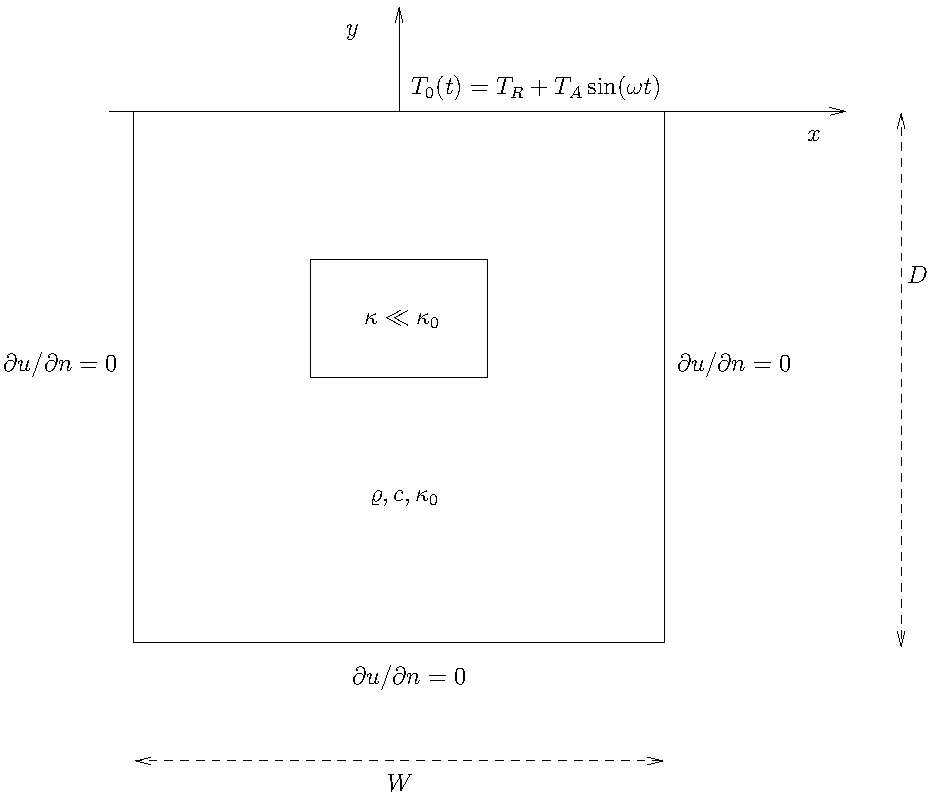
\includegraphics[width=\largefig]{chapters/langtangen/pdf/daynight.pdf}
  \caption{Sketch of a (2D) problem involving heating and cooling of
    the ground due to an oscillating surface temperature}
  \label{langtangen:timedep:diffusion2:sin:fig1}
\end{figure}

The initial-boundary value problem for this problem reads
\begin{align}
\varrho c \frac{\partial T}{\partial t}
    &= \nabla\cdot\left( \kappa\nabla T\right)\hbox{ in }\Omega\times (0,t_{\hbox{stop}}],
\\
T &= T_0(t)\hbox{ on }\Gamma_0,
\\
\frac{\partial T}{\partial n} &= 0\hbox{ on }\partial\Omega\backslash\Gamma_0,
\\
T &= T_R\hbox{ at }t =0.
\end{align}
Here, $\varrho$ is the density of the soil, $c$ is the heat capacity,
$\kappa$ is the thermal conductivity (heat conduction coefficient)
in the soil, and $\Gamma_0$ is the surface boundary $x_{d-1}=0$.

We use a $\theta$-scheme in time; that is, the evolution equation
$\partial P/\partial t=Q(t)$ is discretized as
\begin{equation}
   \frac{P^k - P^{k-1}}{\dt} = \theta Q^k + (1-\theta )Q^{k-1},
\end{equation}
where $\theta\in[0,1]$ is a weighting factor: $\theta =1$
corresponds to the backward difference scheme, $\theta =1/2$ to the
Crank--Nicolson scheme, and $\theta =0$ to a forward difference scheme.
The $\theta$-scheme applied to our PDE results in
\begin{equation}
\varrho c \frac{T^k-T^{k-1}}{\dt} =
\theta \nabla\cdot\left( \kappa\nabla T^k\right)
+ (1-\theta) \nabla\cdot\left( k\nabla T^{k-1}\right).
\end{equation}
Bringing this time-discrete PDE into weak form follows the technique
shown many times earlier in this tutorial. In the standard notation
$a(T,v)=L(v)$ the weak form has
\begin{align}
a(T,v) &= \int_\Omega
\left( \varrho c Tv + \theta{\dt} \kappa\nabla T\cdot \nabla v\right)\dx,
\\
L(v) &= \int_\Omega \left( \varrho c T^{k-1}v - (1-\theta){\dt}
\kappa\nabla T^{k-1}\cdot \nabla v\right)\dx.
\end{align}
Observe that boundary integrals vanish because of the Neumann boundary
conditions.

The size of a 3D box is taken as $W \times W \times D$, where
$D$ is the depth and $W=D/2$ is the width.  \index{heterogeneous
media}\index{multi-material domain} We give the degree of the basis
functions at the command-line, then $D$, and then the divisions of the
domain in the various directions.  To make a box, rectangle, or interval
of arbitrary (not unit) size, we have the \dolfin{} classes \emp{Box},
\emp{Rectangle}, and \emp{Interval} at our disposal. The mesh and the
function space can be created by the following code:
\begin{python}
degree = int(sys.argv[1])
D = float(sys.argv[2])
W = D/2.0
divisions = [int(arg) for arg in sys.argv[3:]]
d = len(divisions)  # no of space dimensions
if d == 1:
    mesh = Interval(divisions[0], -D, 0)
elif d == 2:
    mesh = Rectangle(-W/2, -D, W/2, 0, divisions[0], divisions[1])
elif d == 3:
    mesh = Box(-W/2, -W/2, -D, W/2, W/2, 0,
               divisions[0], divisions[1], divisions[2])
V = FunctionSpace(mesh, "Lagrange", degree)
\end{python}
The \emp{Rectangle} and \emp{Box} objects are defined by the coordinates
of the ``minimum'' and ``maximum'' corners.

Setting Dirichlet conditions at the upper boundary can be done by
\begin{python}
T_R = 0; T_A = 1.0; omega = 2*pi

T_0 = Expression("T_R + T_A*sin(omega*t)",
                 T_R=T_R, T_A=T_A, omega=omega, t=0.0)

def surface(x, on_boundary):
    return on_boundary and abs(x[d-1]) < 1E-14

bc = DirichletBC(V, T_0, surface)
\end{python}

The $\kappa$ function can be defined as a constant $\kappa_1$ inside
the particular rectangular area with a special soil composition, as
indicated in Figure~\ref{langtangen:timedep:diffusion2:sin:fig1}. Outside
this area $\kappa$ is a constant $\kappa_0$.
The domain of the rectangular area is taken as
\[ [-W/4, W/4]\times [-W/4, W/4]\times [-D/2, -D/2 + D/4]\]
in 3D, with $[-W/4, W/4]\times [-D/2, -D/2 + D/4]$ in 2D and
$[-D/2, -D/2 + D/4]$ in 1D.
Since we need some testing in the definition of the $\kappa(x)$
function, the most straightforward approach is to define a subclass
of \emp{Expression}, where we can use a full Python method instead of
just a C++ string formula for specifying a function.
The method that defines the function is called \emp{eval}:
\begin{python}
class Kappa(Function):
    def eval(self, value, x):
        """x: spatial point, value[0]: function value."""
        d = len(x)  # no of space dimensions
        material = 0  # 0: outside, 1: inside
        if d == 1:
            if -D/2. < x[d-1] < -D/2. + D/4.:
                material = 1
        elif d == 2:
            if -D/2. < x[d-1] < -D/2. + D/4. and \
               -W/4. < x[0] < W/4.:
                material = 1
        elif d == 3:
            if -D/2. < x[d-1] < -D/2. + D/4. and \
               -W/4. < x[0] < W/4. and -W/4. < x[1] < W/4.:
                material = 1
        value[0] = kappa_0 if material == 0 else kappa_1
\end{python}
The \emp{eval} method gives great flexibility in defining functions, but a
downside is that C++ calls up \emp{eval} in Python for each point \emp{x},
which is a slow process, and the number of calls is proportional to the
number of nodes in the mesh.  Function expressions in terms of strings
are compiled to efficient C++ functions, being called from C++, so we
should try to express functions as string expressions if possible. (The
\emp{eval} method can also be defined through C++ code, but this is
more complicated and not covered here.)  Using inline if-tests in C++,
we can make string expressions for~$\kappa$:
\begin{python}
kappa_str = {}
kappa_str[1] = "x[0] > -D/2 && x[0] < -D/2 + D/4 ? kappa_1 : kappa_0"
kappa_str[2] = "x[0] > -W/4 && x[0] < W/4 "\
               "&& x[1] > -D/2 && x[1] < -D/2 + D/4 ? "\
               "kappa_1 : kappa_0"
kappa_str[3] = "x[0] > -W/4 && x[0] < W/4 "\
               "x[1] > -W/4 && x[1] < W/4 "\
               "&& x[2] > -D/2 && x[2] < -D/2 + D/4 ?"\
               "kappa_1 : kappa_0"

kappa = Expression(kappa_str[d],
                   D=D, W=W, kappa_0=kappa_0, kappa_1=kappa_1)
\end{python}

Let \emp{T} denote the unknown spatial temperature function at the
current time level, and let \emp{T\_1} be the corresponding function
at one earlier time level.
We are now ready to define the initial condition and the \emp{a} and
\emp{L} forms of our problem:
\begin{python}
T_1 = interpolate(Constant(T_R), V)

rho = 1
c = 1
period = 2*pi/omega
t_stop = 5*period
dt = period/20  # 20 time steps per period
theta = 1

T = TrialFunction(V)
v = TestFunction(V)
f = Constant(0)
a = rho*c*T*v*dx + theta*dt*kappa*\
    inner(nabla_grad(T), nabla_grad(v))*dx
L = (rho*c*T_prev*v + dt*f*v -
     (1-theta)*dt*kappa*inner(nabla_grad(T), nabla_grad(v)))*dx

A = assemble(a)
b = None  # variable used for memory savings in assemble calls
T = Function(V)   # unknown at the current time level
\end{python}
We could, alternatively, break \emp{a} and \emp{L} up in subexpressions
and assemble a mass matrix and stiffness matrix, as exemplified in
Section~\ref{langtangen:timedep:diffusion1:noassemble}, to avoid assembly
of \emp{b} at every time level. This modification is straightforward
and left as an exercise. The speed-up can be significant in 3D problems.

The time loop is very similar to what we have displayed in
Section~\ref{langtangen:timedep:diffusion1:impl}:
\begin{python}
t = dt
while t <= t_stop:
    b = assemble(L, tensor=b)
    T_0.t = t
    bc.apply(A, b)
    solve(A, T.vector(), b)
    # visualization statements
    t += dt
    T_prev.assign(T)
\end{python}
The complete code in \emp{sin\_daD.py} contains several
statements related to visualization and animation
of the solution, both as a finite
element field (\emp{plot} calls) and as a curve in the vertical
direction. The code also plots the exact analytical solution,
\begin{equation}
T(x,t) = T_R + T_Ae^{ax}\sin (\omega t + ax),\quad a =\sqrt \frac{\omega\varrho c}{2\kappa},
\end{equation}
which is valid when $\kappa = \kappa_0=\kappa_1$.

Implementing this analytical solution as a Python function
taking scalars and numpy arrays as arguments requires a word of caution.
A straightforward function like
\begin{python}
def T_exact(x):
    a = sqrt(omega*rho*c/(2*kappa_0))
    return T_R + T_A*exp(a*x)*sin(omega*t + a*x)
\end{python}
will not work and result in an error message from UFL. The reason is that
the names \emp{exp} and \emp{sin} are those imported
by the \emp{from dolfin import *} statement, and these names
come from UFL and are aimed at being used in variational forms.
In the \emp{T\_exact} function where \emp{x} may be a scalar or a
\emp{numpy} array, we therefore need to explicitly specify
\emp{numpy.exp} and \emp{numpy.sin}:
\begin{python}
def T_exact(x):
    a = sqrt(omega*rho*c/(2*kappa_0))
    return T_R + T_A*numpy.exp(a*x)*numpy.sin(omega*t + a*x)
\end{python}
%In general, all pure Python functions in FEniCS code that are
%supposed to apply mathematical functions like \emp{exp}, \emp{log},
%\emp{sin}, \emp{cos}, etc., to \emp{numpy} arrays must
%explicitly have the \emp{numpy} prefix (or be imported after
%\emp{from dolfin import *}, but then the UFL versions of
%\emp{exp}, \emp{log}, etc., are gone).

The reader
is encouraged to play around with the code and test out various parameter
sets:
\begin{enumerate}
\item $T_R=0$, $T_A=1$, $\kappa_0 = \kappa_1=0.2$, $\varrho = c = 1$, $\omega = 2\pi$
\item $T_R=0$, $T_A=1$, $\kappa_0=0.2$, $\kappa_1=0.01$, $\varrho = c = 1$, $\omega = 2\pi$
\item $T_R=0$, $T_A=1$, $\kappa_0=0.2$, $\kappa_1=0.001$, $\varrho = c = 1$, $\omega = 2\pi$
\item $T_R=10$ C, $T_A=10$ C,
$\kappa_0= 2.3 \hbox{ K}^{-1}\hbox{Ns}^{-1}$,
$\kappa_1= 100 \hbox{ K}^{-1}\hbox{Ns}^{-1}$,
$\varrho = 1500\hbox{ kg/m}^3$,
$c = 1600\hbox{ Nm\,kg}^{-1}\hbox{K}^{-1}$,
$\omega = 2\pi/24$ 1/h  $= 7.27\cdot 10^{-5}$ 1/s, $D=1.5$ m
\item As above, but $\kappa_0= 12.3 \hbox{ K}^{-1}\hbox{Ns}^{-1}$ and
$\kappa_1= 10^4 \hbox{ K}^{-1}\hbox{Ns}^{-1}$
\end{enumerate}
Data set no.~4 is relevant for real temperature variations in
the ground (not necessarily the large value of $\kappa_1$), while data set no.~5
exaggerates the effect of a large heat conduction contrast so that
it becomes clearly visible in an animation.


\section{Creating more complex domains}
\label{langtangen:prepro}

Up to now we have been very fond of the unit square as domain, which is
an appropriate choice for initial versions of a PDE solver. The strength
of the finite element method, however, is its ease of handling domains
with complex shapes. This section shows some methods that can be used
to create different types of domains and meshes.

Domains of complex shape must normally be constructed in separate
preprocessor programs. Two relevant preprocessors are Triangle for 2D
domains and NETGEN for 3D domains.

\subsection{Built-in mesh generation tools}
\label{langtangen:prepro:builtin}

\dolfin{} has a few tools for creating various types of meshes over domains
with simple shape:
\emp{UnitInterval},
\emp{UnitSquare},
\emp{UnitCube},
\emp{Interval},
\emp{Rectangle},
\emp{Box},
\emp{UnitCircle}, and
\emp{UnitSphere}.
\index{\emp{UnitInterval}}\index{\emp{UnitSphere}}\index{\emp{UnitSquare}}\index{\emp{Interval}}\index{\emp{Rectangle}}\index{\emp{Box}}\index{\emp{UnitCircle}}\index{\emp{UnitCube}}
Some of these names have been briefly met in previous sections.
The hopefully self-explanatory code snippet below summarizes typical
constructions of meshes with the aid of these tools:
\begin{python}
# 1D domains
mesh = UnitInterval(20)     # 20 cells, 21 vertices
mesh = Interval(20, -1, 1)  # domain [-1,1]

# 2D domains (6x10 divisions, 120 cells, 77 vertices)
mesh = UnitSquare(6, 10)  # "right" diagonal is default
# The diagonals can be right, left or crossed
mesh = UnitSquare(6, 10, "left")
mesh = UnitSquare(6, 10, "crossed")

# Domain [0,3]x[0,2] with 6x10 divisions and left diagonals
mesh = Rectangle(0, 0, 3, 2, 6, 10, "left")

# 6x10x5 boxes in the unit cube, each box gets 6 tetrahedra:
mesh = UnitCube(6, 10, 5)

# Domain [-1,1]x[-1,0]x[-1,2] with 6x10x5 divisions
mesh = Box(-1, -1, -1, 1, 0, 2, 6, 10, 5)

# 10 divisions in radial directions
mesh = UnitCircle(10)
mesh = UnitSphere(10)
\end{python}

\subsection{Transforming mesh coordinates}
\label{langtangen:mesh:transform:cyl}
\index{mesh!transformation}
\index{coordinate stretching}
\index{coordinate transformation}

A mesh that is denser toward a boundary is often desired to increase
accuracy in that region. Given a mesh with uniformly spaced coordinates
$x_0,\ldots,x_{M-1}$ in $[a,b]$, the coordinate transformation $\xi =
(x-a)/(b-a)$ maps $x$ onto $\xi\in [0,1]$. A new mapping $\eta = \xi^s$,
for some $s>1$, stretches the mesh toward $\xi=0$ ($x=a$), while $\eta
= \xi^{1/s}$ makes a stretching toward $\xi=1$ ($x=b$).  Mapping the
$\eta\in[0,1]$ coordinates back to $[a,b]$ gives new, stretched $x$
coordinates,
\begin{equation}
  \bar x = a + (b-a)\left( \brac{x-a}{b-a}\right)^s
\end{equation}
toward $x=a$, or
\begin{equation}
  \bar x = a + (b-a)\left(\frac{x-a}{b-a}\right)^{1/s}
\end{equation}
toward $x=b$

One way of creating more complex geometries is to transform the
vertex coordinates in a rectangular mesh according to some formula.
Say we want to create a part of a hollow cylinder of $\Theta$ degrees,
with inner radius $a$ and outer radius $b$. A standard mapping from
polar coordinates to Cartesian coordinates can be used to generate the
hollow cylinder. Given a rectangle in $(\bar x, \bar y)$ space such
that $a\leqslant \bar x\leqslant b$ and $0\leqslant \bar y\leqslant 1$,
the mapping
\begin{equation}
 \hat x = \bar x\cos (\Theta \bar y),\quad \hat y
    = \bar x\sin (\Theta \bar y),
\end{equation}
takes a point in the rectangular $(\bar x,\bar y)$ geometry and maps it
to a point $(\hat x, \hat y)$ in a hollow cylinder.

The corresponding Python code for first stretching the mesh and then
mapping it onto a hollow cylinder looks as follows:
\begin{python}
Theta = pi/2
a, b = 1, 5.0
nr = 10  # divisions in r direction
nt = 20  # divisions in theta direction
mesh = Rectangle(a, 0, b, 1, nr, nt, "crossed")

# First make a denser mesh towards r=a
x = mesh.coordinates()[:,0]
y = mesh.coordinates()[:,1]
s = 1.3

def denser(x, y):
    return [a + (b-a)*((x-a)/(b-a))**s, y]

x_bar, y_bar = denser(x, y)
xy_bar_coor = numpy.array([x_bar, y_bar]).transpose()
mesh.coordinates()[:] = xy_bar_coor
plot(mesh, title="stretched mesh")

def cylinder(r, s):
    return [r*numpy.cos(Theta*s), r*numpy.sin(Theta*s)]

x_hat, y_hat = cylinder(x_bar, y_bar)
xy_hat_coor = numpy.array([x_hat, y_hat]).transpose()
mesh.coordinates()[:] = xy_hat_coor
plot(mesh, title="hollow cylinder")
interactive()
\end{python}
The result of calling \emp{denser} and \emp{cylinder} above is a
list of two vectors, with the $x$ and $y$ coordinates, respectively.
Turning this list into a \emp{numpy} array object results in a $2\times
M$ array, $M$ being the number of vertices in the mesh. However,
\emp{mesh.coordinates()} is by a convention an $M\times 2$ array so
we need to take the transpose. The resulting mesh is displayed in
Figure~\ref{langtangen:mesh:transform:cyl:fig1}.
\begin{figure}
\bwfig
 \centering
 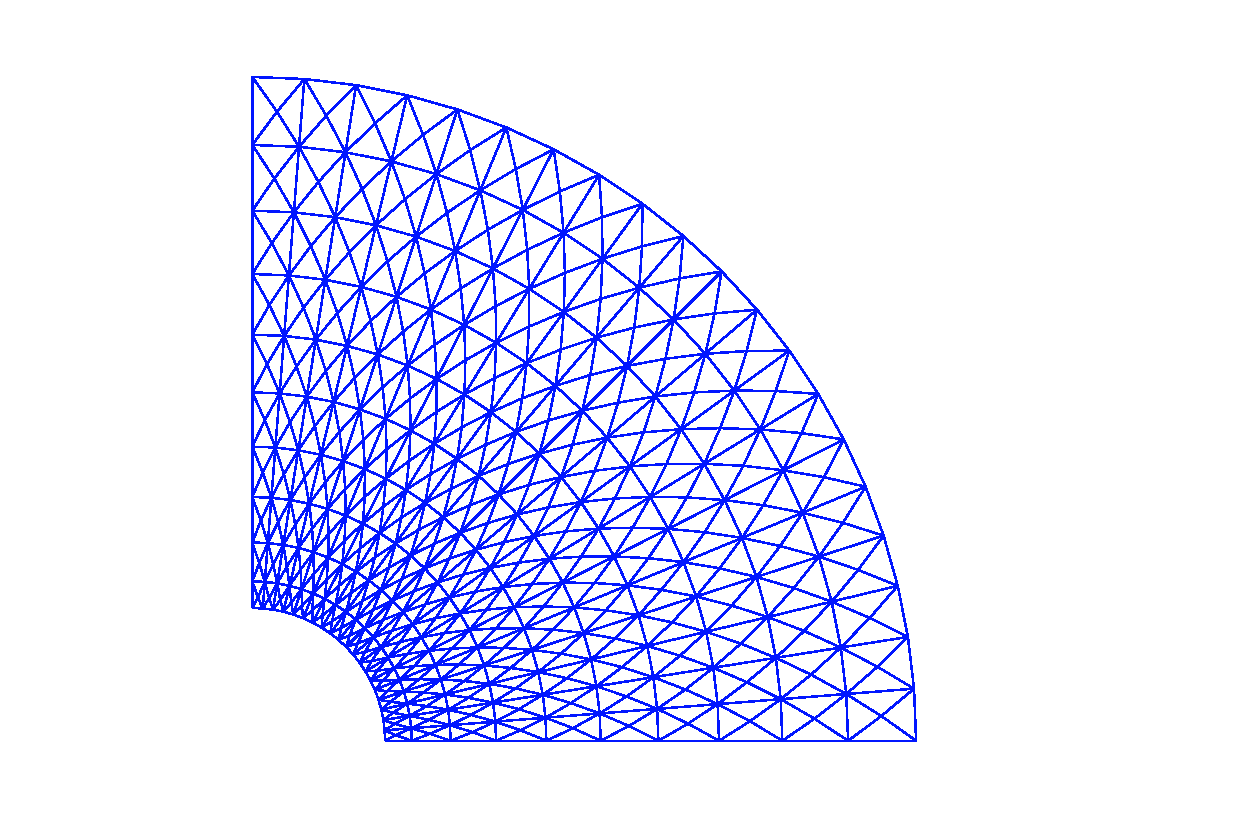
\includegraphics[width=\largefig]{chapters/langtangen/pdf/hollow_cylinder.pdf}
  \caption{A hollow cylinder generated by mapping a rectangular mesh,
  stretched toward the left side.}
\label{langtangen:mesh:transform:cyl:fig1}
\end{figure}

Setting boundary conditions in meshes created from mappings like the
one illustrated above is most conveniently done by using a mesh function
to mark parts of the boundary. The marking is easiest to perform before
the mesh is mapped since one can then conceptually work with the sides
in a pure rectangle.

\section{Handling domains with different materials}
\index{heterogeneous media}\index{multi-material domain}

Solving PDEs in domains made up of different materials is a frequently
encountered task. In \fenics, these kind of problems are handled by
defining subdomains inside the domain. The subdomains may represent
the various materials. We can thereafter define material properties
through functions, known in \fenics{} as \emph{mesh functions}, that are
piecewise constant in each subdomain.  A simple example with two materials
(subdomains) in 2D will demonstrate the basic steps in the process.

\subsection{Working with two subdomains}
\label{langtangen:possion:2D:2mat:problem}

Suppose we want to solve
\begin{equation} \label{langtangen:poisson:2D:2mat:varcoeff2}
  \nabla\cdot \left\lbrack k(x,y)\nabla u(x,y)\right\rbrack = 0,
\end{equation}
in a domain $\Omega$ consisting of two subdomains where $k$ takes on
a different value in each subdomain.
For simplicity, yet without loss of generality, we choose for the current
implementation
the domain $\Omega = [0,1]\times [0,1]$ and divide it into two equal
subdomains, as depicted in Figure~\ref{langtangen:possion:2D:2mat:fig1},
\begin{equation}
 \Omega_0 = [0, 1]\times [0,1/2],\quad \Omega_1 = [0, 1]\times (1/2,1].
\end{equation}
We define $k(x,y)=k_0$ in $\Omega_0$ and $k(x,y)=k_1$ in $\Omega_1$,
where $k_0>0$ and $k_1>0$ are given constants.  As boundary conditions,
we choose $u=0$ at $y=0$, $u=1$ at $y=1$, and $\partial u/\partial n=0$
at $x=0$ and $x=1$.  One can show that the exact solution is now given by
\begin{equation}
u(x, y) = \left\lbrace\begin{array}{ll}
\frac{2yk_1}{k_0+k_1}, & y \leqslant 1/2\\
\frac{(2y-1)k_0 + k_1}{k_0+k_1}, & y \geqslant 1/2
\end{array}\right.
\end{equation}
As long as the element boundaries coincide with the internal boundary
$y=1/2$, this piecewise linear solution should be exactly recovered
by Lagrange elements of any degree. We use this property to verify the
implementation.

\begin{figure}
% NOTE: remove everything with \SetFigFont etc. from xfig
\newcommand{\SetFigFontNFSS}[2]{}
  \centerline{
%\setlength{\unitlength}{4144sp}
\setlength{\unitlength}{2144sp}
% no blank line before begin{picture}
\begin{picture}(6372,6030)(166,-6376)
\thinlines
{\color[rgb]{0,0,0}\put(901,-5956){\vector( 0, 1){5445}}
}%
{\color[rgb]{0,0,0}\put(901,-5911){\vector( 1, 0){5625}}
}%
{\color[rgb]{0,0,0}\put(901,-2086){\line( 1, 0){3825}}
\put(4726,-2086){\line( 0,-1){3825}}
}%
{\color[rgb]{0,0,0}\put(901,-4021){\line( 1, 0){3825}}
}%
\put(6301,-6226){$x$}
\put(586,-601){$y$}
%\put(2251,-6361){$\partial u/\partial n=0$}
%\put(2251,-1861){$\partial u/\partial n=0$}
%\put(2300,-6361){$u=0$}
%\put(2300,-1861){$u=1$}
\put(2520,-6361){$u=0$}
\put(2520,-1861){$u=1$}
%\put(2431,-3211){$\Omega_1$}
%\put(2476,-5191){$\Omega_0$}
\put(2700,-3211){$\Omega_1$}
\put(2700,-5050){$\Omega_0$}
%\put(181,-4156){$u=0$}
\put(-40,-4111){$\frac{\partial u}{\partial n}=0$}
\put(4861,-4111){$\frac{\partial u}{\partial n}=0$}
\end{picture}%
  }
 \caption{Sketch of a Poisson problem with a variable coefficient that
 is constant in each of the two subdomains $\Omega_0$ and $\Omega_1$.}
\label{langtangen:possion:2D:2mat:fig1}
\end{figure}

Physically, the present problem may correspond to heat conduction, where
the heat conduction in $\Omega_1$ is ten times more efficient than in
$\Omega_0$. An alternative interpretation is flow in porous media with
two geological layers, where the layers' ability to transport the fluid
differs by a factor of 10.

\subsection{Implementation}
\label{langtangen:possion:2D:2mat:impl}

The new functionality in this subsection regards how to define
the subdomains $\Omega_0$ and $\Omega_1$. For this purpose we need to
use subclasses of class \emp{SubDomain},
not only plain functions as we have used so far for specifying
boundaries. Consider the boundary function
\begin{python}
def boundary(x, on_boundary):
    tol = 1E-14
    return on_boundary and abs(x[0]) < tol
\end{python}
for defining the boundary $x=0$. Instead of using such a stand-alone
function, we can create an instance\footnote{The term \emph{instance}
means a Python object of a particular type (such as \emp{SubDomain},
\emp{Function}, \emp{FunctionSpace}, etc.).  Many use \emph{instance}
and \emph{object} as interchangeable terms. In other computer programming
languages one may also use the term \emph{variable} for the same thing.
We mostly use the well-known term \emph{object} in this text.} of a
subclass of \emp{SubDomain}, which implements the \emp{inside} method
as an alternative to the \emp{boundary} function:
\begin{python}
class Boundary(SubDomain):
    def inside(x, on_boundary):
        tol = 1E-14
        return on_boundary and abs(x[0]) < tol

boundary = Boundary()
bc = DirichletBC(V, Constant(0), boundary)
\end{python}

A subclass of \emp{SubDomain} with an \emp{inside} method offers
functionality for marking parts of the domain or the boundary. Now
we need to define one class for the subdomain $\Omega_0$ where $y\leqslant
1/2$ and another for the subdomain $\Omega_1$ where $y\geqslant 1/2$:
\begin{python}
class Omega0(SubDomain):
    def inside(self, x, on_boundary):
        return True if x[1] <= 0.5 else False

class Omega1(SubDomain):
    def inside(self, x, on_boundary):
        return True if x[1] >= 0.5 else False
\end{python}
Notice the use of \emp{<=} and \emp{>=} in both tests. For a cell
to belong to, e.g., $\Omega_1$, the \emp{inside} method must return
\emp{True} for all the vertices \emp{x} of the cell. So to make the cells
at the internal boundary $y=1/2$ belong to $\Omega_1$, we need the test
\emp{x[1] >= 0.5}.

The next task is to use a \emp{MeshFunction} to mark all cells in
$\Omega_0$ with the subdomain number 0 and all cells in $\Omega_1$
with the subdomain number 1.  Our convention is to number subdomains
as $0,1,2,\ldots$.
%To make programs more readable, we may introduce logical names for
%the subdomain numbers, e.g., \emp{LOWER} for no.~0 and
%\emp{UPPER} for no.~1 in our case\footnote{It is common to
%use upper case letters in name for constants that correspond to integers (known
%as \emph{enum} types).}.

A \emp{MeshFunction} is a discrete function that can be evaluated at a
set of so-called \emph{mesh entities}. Examples of mesh entities are cells,
facets, and vertices. A \emp{MeshFunction} over cells is suitable
to represent subdomains (materials), while a \emp{MeshFunction} over
facets is used to represent pieces of external or internal boundaries.
Mesh functions over vertices can be used to describe continuous fields.

Since we need to define subdomains of $\Omega$ in the present example, we
must make use of a \emp{MeshFunction} over cells. The \emp{MeshFunction}
constructor is fed with three arguments: 1) the type of value:
\emp{"int"} for integers, \emp{"uint"} for positive (unsigned) integers,
\emp{"double"} for real numbers, and \emp{"bool"} for logical values; 2)
a \emp{Mesh} object, and 3) the topological dimension of the mesh entity
in question: cells have topological dimension equal to the number of
space dimensions in the PDE problem, and facets have one dimension lower.
Alternatively, the constructor can take just a filename and initialize
the \emp{MeshFunction} from data in a file.

We start with creating a \emp{MeshFunction} whose values are non-negative
integers (\emp{"uint"}) for numbering the subdomains.  The mesh entities
of interest are the cells, which have dimension 2 in a two-dimensional
problem (1 in 1D, 3 in 3D). The appropriate code for defining the
\emp{MeshFunction} for two subdomains then reads
\begin{python}
subdomains = MeshFunction("uint", mesh, 2)
# Mark subdomains with numbers 0 and 1
subdomain0 = Omega0()
subdomain0.mark(subdomains, 0)
subdomain1 = Omega1()
subdomain1.mark(subdomains, 1)
\end{python}

Calling \emp{subdomains.array()} returns a \emp{numpy} array of the
subdomain values. That is,\break \emp{subdomain.array()[i]} is the subdomain
value of cell number \emp{i}. This array is used to look up the subdomain
or material number of a specific element.

We need a function \emp{k} that is constant in each subdomain $\Omega_0$
and $\Omega_1$. Since we want \emp{k} to be a finite element function,
it is natural to choose a space of functions that are constant over each
element.  The family of discontinuous Galerkin methods, in \fenics{}
denoted by \emp{"DG"}, is suitable for this purpose. Since we want
functions that are piecewise constant, the value of the degree parameter
is zero:
\begin{python}
V0 = FunctionSpace(mesh, "DG", 0)
k  = Function(V0)
\end{python}
To fill \emp{k} with the right values in each element, we loop over all
cells (the indices in \emp{subdomain.array()}), extract the corresponding
subdomain number of a cell, and assign the corresponding $k$ value to
the \emp{k.vector()} array:
\begin{python}
k_values = [1.5, 50]  # values of k in the two subdomains
for cell_no in range(len(subdomains.array())):
    subdomain_no = subdomains.array()[cell_no]
    k.vector()[cell_no] = k_values[subdomain_no]
\end{python}

Long loops in Python are known to be slow, so for large meshes it is
preferable to avoid such loops and instead use \emph{vectorized code}.
Normally this implies that the loop must be replaced by calls to
functions from the \emp{numpy} library that operate on complete arrays
(in efficient C code). The functionality we want in the present case
is to compute an array of the same size as \emp{subdomain.array()},
but where the value \emp{i} of an entry in \emp{subdomain.array()}
is replaced by \emp{k\_values[i]}.  Such an operation is carried out by
the \emp{numpy} function \emp{choose}:
\begin{python}
help = numpy.asarray(subdomains.array(), dtype=numpy.int32)
k.vector()[:] = numpy.choose(help, k_values)
\end{python}
The \emp{help} array is required since \emp{choose} cannot work with
\emp{subdomain.array()} because this array has elements of type
\emp{uint32}. We must therefore transform this array to an array
\emp{help} with standard \emp{int32} integers.

Having the \emp{k} function ready for finite element
computations, we can proceed in the normal manner
with defining essential boundary conditions, as in
Section~\ref{langtangen:poisson:multiple:Dirichlet}, and the $a(u,v)$
and $L(v)$ forms, as in Section~\ref{langtangen:possion:2D:varcoeff}.
All the details can be found in the file \emp{mat2\_p2D.py}.

\subsection{Multiple Neumann, Robin, and Dirichlet conditions}
\label{langtangen:poisson:mat:neumann}
\index{boundary condition!Dirichlet}
\index{boundary condition!Neumann}
\index{boundary condition!Robin}
\index{boundary condition}

Let us go back to the model problem from
Section~\ref{langtangen:poisson:multiple:Dirichlet} where we had both
Dirichlet and Neumann conditions.  The term \emp{v*g*ds} in the expression
for \emp{L} implies a boundary integral over the complete boundary,
or in \fenics{} terms, an integral over all exterior facets.
However, the contributions from the parts of the boundary where we have
Dirichlet conditions are erased when the linear system is modified by the
Dirichlet conditions.  We would like, from an efficiency point of view,
to integrate \emp{v*g*ds} only over the parts of the boundary where
we actually have Neumann conditions.  And more importantly, in other
problems one may have different Neumann conditions or other conditions
like the Robin type condition.  With the mesh function concept we can
mark different parts of the boundary and integrate over specific parts.
The same concept can also be used to treat multiple Dirichlet conditions.
The forthcoming text illustrates how this is done.

Essentially, we still stick to the model problem from
Section~\ref{langtangen:poisson:multiple:Dirichlet}, but replace the
Neumann condition at $y=0$ by a \emph{Robin condition}\footnote{The Robin
condition is most often used to model heat transfer to the surroundings
and arise naturally from Newton's cooling law.}:
\begin{equation}
 - \frac{\partial u}{\partial n} = p(u-q),
\end{equation}
where $p$ and $q$ are specified functions.  Since we have prescribed
a simple solution in our model problem, $u=1+x^2+2y^2$, we adjust
$p$ and $q$ such that the condition holds at $y=0$. This implies that
$q=1+x^2+2y^2$ and $p$ can be arbitrary (the normal derivative at $y=0$:
$\partial u/\partial n = -\partial u/\partial y = -4y=0$).

Now we have four parts of the boundary: $\Gamma_{\mathrm{N}}$ which corresponds
to the upper side $y=1$, $\Gamma_R$ which corresponds to the lower part
$y=0$, $\Gamma_0$ which corresponds to the left part $x=0$, and $\Gamma_1$
which corresponds to the right part $x=1$. The complete boundary-value
problem reads
\begin{align}
  - \Delta u &= -6 \mbox{ in } \Omega,
  \label{langtangen:poisson:2D:DN3}
\\
  u &= u_L \mbox{ on } \Gamma_0,
  \label{langtangen:poisson:2D:DN3:bc1}
\\
  u &= u_R \mbox{ on } \Gamma_1,
  \label{langtangen:poisson:2D:DN3:bc2}
\\
  - \frac{\partial u}{\partial n} &= p(u-q) \mbox{ on } \Gamma_R,
  \label{langtangen:poisson:2D:DN3:bc3}
\\
  - \frac{\partial u}{\partial n} &= g \mbox{ on } \Gamma_{\mathrm{N}}.
  \label{langtangen:poisson:2D:DN3:bc4}
\end{align}
The involved prescribed functions are $u_L= 1 + 2y^2$, $u_R = 2 + 2y^2$,
$q=1+x^2+2y^2$, $p$ is arbitrary, and $g=-4y$.

Integration by parts of $-\int_\Omega v\Delta u\dx$ becomes as usual
\begin{equation}
 -\int_\Omega v\Delta u \dx
= \int_\Omega\nabla u\cdot \nabla v\dx
  - \int_{\partial\Omega} \frac{\partial u}{\partial n}v\ds.
\end{equation}
The boundary integral vanishes on $\Gamma_0\cup\Gamma_1$, and we split the
parts over $\Gamma_{\mathrm{N}}$ and $\Gamma_R$ since we have different conditions
at those parts:
\begin{equation}
- \int_{\partial\Omega}v \frac{\partial u}{\partial n}\ds
=
-\int_{\Gamma_{\mathrm{N}}}v \frac{\partial u}{\partial n}\ds
 - \int_{\Gamma_R}v \frac{\partial u}{\partial n}\ds
= \int_{\Gamma_{\mathrm{N}}}vg\ds
+ \int_{\Gamma_R}vp(u-q)\ds.
\end{equation}
The weak form then becomes
\begin{equation}
\int_{\Omega} \nabla u\cdot \nabla v \dx
+ \int_{\Gamma_{\mathrm{N}}} gv\ds + \int_{\Gamma_R}p(u-q)v\ds
= \int_{\Omega} fv \dx,
\end{equation}
We want to write this weak form in the standard notation $a(u,v)=L(v)$,
which requires that we identify all integrals with \emph{both} $u$ and
$v$, and collect these in $a(u,v)$, while the remaining integrals with
$v$ and not $u$ go into $L(v)$.  The integral from the Robin condition
must of this reason be split in two parts:
\begin{equation}
 \int_{\Gamma_R}p(u-q)v\ds
= \int_{\Gamma_R}puv\ds - \int_{\Gamma_R}pqv\ds.
\end{equation}
We then have
\begin{align}
  a(u, v) &= \int_{\Omega} \nabla u\cdot \nabla v \dx
    + \int_{\Gamma_R}puv\ds,
  \label{langtangen:poisson:2D:DN3:var:a}
\\
  L(v) &= \int_{\Omega} fv \dx - \int_{\Gamma_{\mathrm{N}}} g v\ds + \int_{\Gamma_R}pqv\ds.
  \label{langtangen:poisson:2D:DN3:var:L}
\end{align}

A natural starting point for implementation is the
file \emp{stationary/poisson/dn2\_p2D.py}.
The new aspects are
\begin{enumerate}
\item definition of a mesh function over the boundary,
\item marking each side as a subdomain, using the mesh function,
\item splitting a boundary integral into parts.
\end{enumerate}
%%
Task 1 makes use of the \emp{MeshFunction} object, but contrary to
Section~\ref{langtangen:possion:2D:2mat:impl}, this is not a function
over cells, but a function over cell facets. The topological dimension of
cell facets is one lower than the cell interiors, so in a two-dimensional
problem the dimension becomes 1. In general, the facet dimension is given
as \emp{mesh.topology().dim()-1}, which we use in the code for ease of
direct reuse in other problems.  The construction of a \emp{MeshFunction}
object to mark boundary parts now reads
\begin{python}
boundary_parts = \
  MeshFunction("uint", mesh, mesh.topology().dim()-1)
\end{python}
As in Section~\ref{langtangen:possion:2D:2mat:impl} we use a
subclass of \emp{SubDomain} to identify the various parts of the mesh
function. Problems with domains of more complicated geometries may set
the mesh function for marking boundaries as part of the mesh generation.
In our case, the $y=0$ boundary can be marked by
\begin{python}
class LowerRobinBoundary(SubDomain):
    def inside(self, x, on_boundary):
        tol = 1E-14   # tolerance for coordinate comparisons
        return on_boundary and abs(x[1]) < tol

Gamma_R = LowerRobinBoundary()
Gamma_R.mark(boundary_parts, 0)
\end{python}
The code for the $y=1$ boundary is similar and is seen in
\emp{dnr\_p2D}.

The Dirichlet boundaries are marked similarly, using subdomain number
2 for $\Gamma_0$ and 3 for~$\Gamma_1$:
\begin{python}
class LeftBoundary(SubDomain):
    def inside(self, x, on_boundary):
        tol = 1E-14   # tolerance for coordinate comparisons
        return on_boundary and abs(x[0]) < tol

Gamma_0 = LeftBoundary()
Gamma_0.mark(boundary_parts, 2)

class RightBoundary(SubDomain):
    def inside(self, x, on_boundary):
        tol = 1E-14   # tolerance for coordinate comparisons
        return on_boundary and abs(x[0] - 1) < tol

Gamma_1 = RightBoundary()
Gamma_1.mark(boundary_parts, 3)
\end{python}
Specifying the \emp{DirichletBC} objects may now make use of the mesh
function (instead of a \emp{SubDomain} subclass object) and an indicator
for which subdomain each condition should be applied to:
\begin{python}
u_L = Expression("1 + 2*x[1]*x[1]")
u_R = Expression("2 + 2*x[1]*x[1]")
bcs = [DirichletBC(V, u_L, boundary_parts, 2),
       DirichletBC(V, u_R, boundary_parts, 3)]
\end{python}

Some functions need to be defined before we can go on with the \emp{a}
and \emp{L} of the variational problem:
\begin{python}
g = Expression("-4*x[1]")
q = Expression("1 + x[0]*x[0] + 2*x[1]*x[1]")
p = Constant(100)  # arbitrary function can go here
u = TrialFunction(V)
v = TestFunction(V)
f = Constant(-6.0)
\end{python}

The new aspect of the variational problem is the two distinct boundary
integrals.  Having a mesh function over exterior cell facets (our
\emp{boundary\_parts} object), where subdomains (boundary parts) are
numbered as $0,1,2,\ldots$, the special symbol \emp{ds(0)} implies
integration over subdomain (part) 0, \emp{ds(1)} denotes integration
over subdomain (part) 1, and so on.  The idea of multiple \emp{ds}-type
objects generalizes to volume integrals too: \emp{dx(0)}, \emp{dx(1)},
etc., are used to integrate over subdomain 0, 1, etc., inside $\Omega$.

The variational problem can be defined as
\begin{python}
a = inner(nabla_grad(u), nabla_grad(v))*dx + p*u*v*ds(0)
L = f*v*dx - g*v*ds(1) + p*q*v*ds(0)
\end{python}
For the \emp{ds(0)} and \emp{ds(1)} symbols to work we must obviously
connect them (or \emp{a} and \emp{L}) to the mesh function marking
parts of the boundary. This is done by a certain keyword argument to
the \emp{assemble} function:
\begin{python}
A = assemble(a, exterior_facet_domains=boundary_parts)
b = assemble(L, exterior_facet_domains=boundary_parts)
\end{python}
Then essential boundary conditions are enforced, and the system can be
solved in the usual way:
\begin{python}
for bc in bcs: bc.apply(A, b)
u = Function(V)
U = u.vector()
solve(A, U, b)
\end{python}
The complete code is in the \emp{dnr\_p2D.py} file in the
\emp{stationary/poisson} directory.

\section{More examples}

Many more topics could be treated in a \fenics{} tutorial, e.g., how
to solve systems of PDEs, how to work with mixed finite element
methods, how to create more complicated meshes and mark boundaries,
and how to create more advanced visualizations.  However, to limit the
size of this tutorial, the examples end here.  There are, fortunately,
a rich set of FEniCS demos.  The FEniCS documentation explains a
collection of PDE solvers in detail: the Poisson equation, the mixed
formulation for the Poisson equation, the Biharmonic equation, the
equations of hyperelasticity, the Cahn-Hilliard equation, and the
incompressible Navier--Stokes equations.  Both Python and C++ versions
of these solvers are explained.  An eigenvalue solver is also
documented.  In the \emp{dolfin/demo} directory of the \dolfin{} source
code tree you can find programs for these and many other examples,
including the advection-diffusion equation, the equations of
elastodynamics, a reaction-diffusion equation, various finite element
methods for the Stokes problem, discontinuous Galerkin methods for the
Poisson and advection-diffusion equations, and an eigenvalue problem
arising from electromagnetic waveguide problem with \nedelec{}
elements.  There are also numerous demos on how to apply various
functionality in FEniCS, e.g., mesh refinement and error control,
moving meshes (for ALE methods), computing functionals over subsets of
the mesh (such as lift and drag on bodies in flow), and creating
separate subdomain meshes from a parent mesh.

The project CBC.Solve (\emp{https://launchpad.net/cbc.solve}) offers
more complete PDE solvers for the Navier--Stokes equations
(Chapter~\ref{chap:selim}), the equations of hyperelasticity
(Chapter~\ref{chap:narayanan}), fluid--structure interaction
(Chapter~\ref{chap:selim}), viscous mantle flow
(Chapter~\ref{chap:vynnytska}), and the bidomain model of
electrophysiology.  Another project, CBC.RANS
(\emp{https://launchpad.net/cbc.rans}), offers an environment for very
flexible and easy implementation
of Navier--Stokes solvers and turbulence
\citet{Mortensen2011,Mortensen2011b}. For example,
CBC.RANS contains an elliptic relaxation model for turbulent flow
involving 18 nonlinear PDEs. FEniCS proved to be an ideal environment
for implementing such complicated PDE models.
The easy construction of systems of nonlinear PDEs in CBC.RANS has been
further generalized to simplify the implementation of large systems
of nonlinear PDEs in general. The functionality is found in the
CBC.PDESys package (\emp{https://launchpad.net/cbcpdesys}).

\section{Miscellaneous topics}


\subsection{Glossary}

Below we explain some key terms used in this tutorial.
%
\begin{trivlist}\leftskip4pt
  \item[\fenics:] name of a software suite composed of many individual
  software components (see\break \emp{fenicsproject.org}). Some components are
  \dolfin{} and Viper, explicitly referred to in this tutorial. Others are
  FFC and FIAT, heavily used by the programs appearing in this tutorial,
  but never explicitly used from the programs.

  \item[DOLFIN:] a \fenics{} component, more precisely a C++ library,
  with a Python interface, for performing important actions in finite
  element programs. \dolfin{} makes use of many other \fenics{} components
  and many external software packages.

  \item[Viper:] a \fenics{} component for quick visualization of finite
  element meshes and solutions.

  \item[UFL:] a \fenics{} component implementing the \emph{unified
  form language} for specifying finite element forms in \fenics{}
  programs.  The definition of the forms, typically called
  \emp{a} and \emp{L} in this tutorial, must have legal UFL
  syntax. The same applies to the definition of functionals (see
  Section~\ref{langtangen:poisson1:functionals}).

  \item[Class (Python):] a programming construction for creating objects
  containing a set of variables and functions. Most types of \fenics{}
  objects are defined through the class concept.

  \item[Instance (Python):] an object of a particular type, where the type
  is implemented as a class. For instance, \emp{mesh = UnitInterval(10)}
  creates an instance of class \emp{UnitInterval}, which is reached by
  the name \emp{mesh}. (Class \emp{UnitInterval} is actually just an
  interface to a corresponding C++ class in the \dolfin{} C++ library.)

  \item[Class method (Python):] a function in a class, reached by dot
  notation: \emp{instance\_name.method\_name}.

  \item[\emp{self} parameter (Python):] required first parameter in class
  methods, representing a particular object of the class.\index{\emp{self}}
  Used in method definitions, but never in calls to a method.  For example,
  if \emp{method(self, x)} is the definition of \emp{method} in a class
  \emp{Y}, \emp{method} is called as \emp{y.method(x)}, where \emp{y}
  is an instance of class \emp{Y}.  In a call like \emp{y.method(x)},
  \emp{method} is invoked with \emp{self=y}.

  \item[Class attribute (Python):] a variable in a class, reached by
  dot notation: \emp{instance\_name.attribute\_\break name}.
\end{trivlist}

\subsection{Overview of objects and functions}

Most classes in \fenics{} have an explanation of the purpose and usage
that can be seen by using the general documentation command \emp{pydoc}
for Python objects. You can type\index{\emp{pydoc}}
\begin{progoutput}
pydoc dolfin.X
\end{progoutput}
%
to look up documentation of a Python class \emp{X} from the \dolfin{}
library (\emp{X} can be \emp{UnitSquare}, \emp{Function}, \emp{FunctionSpace},
etc.). Below is an overview of the most important classes and functions
in \fenics{} programs, in the order they typically appear within
programs.\enlargethispage{12pt}
%
\begin{trivlist}\leftskip3.5pt
  \item[\emp{UnitSquare(nx, ny)}:] generate mesh over the unit square
  $[0,1]\times [0,1]$ using \emp{nx} divisions in $x$ direction and
  \emp{ny} divisions in $y$ direction. Each of the \emp{nx*ny} squares
  are divided into two cells of triangular shape.

  \item[\emp{UnitInterval}, \emp{UnitCube}, \emp{UnitCircle},
  \emp{UnitSphere}, \emp{Interval}, \emp{Rectangle}, and \emp{Box}:]
  generate mesh over domains of simple geometric shape, see
  Section~\ref{langtangen:prepro}.

  \item[\emp{FunctionSpace(mesh, element\_type, degree)}:] a
  function space defined over a mesh, with a given element type (e.g.,
  \emp{"Lagrange"} or \emp{"DG"}), with basis functions as polynomials
  of a specified degree.

  \item[\emp{Expression(formula, p1=v1, p2=v2, ...)}:]
   a scalar- or vector-valued function,
   given as a mathematical expression \emp{formula} (string) written in
   C++ syntax. The spatial coordinates in the expression are named
   \emp{x[0]}, \emp{x[1]}, and \emp{x[2]}, while time and other
   physical parameters can be represented as symbols \emp{p1}, \emp{p2},
   etc., with corresponding values \emp{v1}, \emp{v2}, etc., initialized
   through keyword arguments. These parameters become attributes,
   whose values can be modified when desired.

  \item[\emp{Function(V)}:] a scalar- or vector-valued finite element
  field in the function space \emp{V}. If \emp{V} is a \emp{Function\break Space}
  object, \emp{Function(V)} becomes a scalar field, and with \emp{V}
  as a \emp{VectorFunctionSpace} object, \emp{Function(V)} becomes a
  vector field.

  \item[\emp{SubDomain}:] class for defining a subdomain, either
  a part of the boundary, an internal boundary, or a part of
  the domain.  The programmer must subclass \emp{SubDomain} and
  implement the \emp{inside(self, x, on\_boundary)} function (see
  Section~\ref{langtangen:poisson1:impl}) for telling whether a point
  \emp{x} is inside the subdomain or not.

  \item[\emp{Mesh}:] class for representing a finite element mesh,
  consisting of cells, vertices, and optionally faces, edges, and facets.

  \item[\emp{MeshFunction}:] tool for marking parts of the domain or
  the boundary.  Used for variable coefficients (``material properties'',
  see Section~\ref{langtangen:possion:2D:2mat:problem}) or for boundary
  conditions (see Section~\ref{langtangen:poisson:mat:neumann}).

  \item[\emp{DirichletBC(V, value, where)}:] specification of Dirichlet
  (essential) boundary conditions via a function space \emp{V}, a
  function \emp{value(x)} for computing the value of the condition at
  a point \emp{x}, and a specification \emp{where} of the boundary,
  either as a \emp{SubDomain} subclass instance, a plain function, or
  as a \emp{MeshFunction} instance.  In the latter case, a 4th argument
  is provided to describe which subdomain number that describes the
  relevant boundary.

  \item[\emp{TrialFunction(V)}:] define a trial function on a space
  \emp{V} to be used in a variational form to represent the unknown in
  a finite element problem.

  \item[\emp{TestFunction(V)}:] define a test function on a space \emp{V}
  to be used in a variational form.

  \item[\emp{assemble(X)}:] assemble a matrix, a right-hand side, or a
  functional, given a from \emp{X} written with UFL syntax.

  \item[\emp{assemble\_system(a, L, bcs)}:] assemble the matrix and the
  right-hand side from a bilinear (\emp{a}) and linear (\emp{L}) form
  written with UFL syntax. The \emp{bcs} parameter holds one or more
  \emp{DirichletBC} objects.

  \item[\emp{LinearVariationalProblem(a, L, u, bcs)}:]
  define a variational problem,
  given a bilinear (\emp{a}) and linear (\emp{L}) form, written with UFL
  syntax, and one or more \emp{DirichletBC} objects stored in \emp{bcs}.

  \item[\emp{LinearVariationalSolver(problem)}:] create solver object for
  a a linear variational problem object (\emp{problem}).

  \item[\emp{solve(A, U, b)}:] solve a linear system with \emp{A}
  as coefficient matrix (\emp{Matrix} object), \emp{U} as unknown
  (\emp{Vector} object), and \emp{b} as right-hand side (\emp{Vector}
  object).  Usually, \emp{U = u.vector()}, where
  \emp{u} is a \emp{Function} object representing the unknown finite
  element function of the problem, while \emp{A} and \emp{b} are computed
  by calls to \emp{assemble} or \emp{assemble\_system}.

  \item[\emp{plot(q)}:] quick visualization of a mesh, function, or mesh
  function \emp{q}, using the Viper component in \fenics{}.

  \item[\emp{interpolate(func, V)}:] interpolate a formula or finite
  element function \emp{func} onto the function space \emp{V}.

  \item[\emp{project(func, V)}:] project a formula or finite element
  function \emp{func} onto the function space \emp{V}.
\end{trivlist}

\subsection{User-defined functions}
\label{langtangen:app:cpp:functions}

%outdated:
%User-defined functions are implemented as a \emp{Function} object.
%There are several ways of constructing such objects, such as
%\begin{itemize}
%\item a string containing a mathematical expression,
%\item a subclass of \emp{Function} in Python,
%\item a subclass of \emp{Function} in C++,
%\item a set of degrees of freedom of a finite element function.
%\end{itemize}
%Writing \emp{pydoc dolfin.Function} gives a documentation of the various
%techniques.

When defining a function in terms of a mathematical expression inside
a string formula, e.g.,
\begin{python}
myfunc = Expression("sin(x[0])*cos(x[1])")
\end{python}
the expression contained in the first argument will be turned into a C++
function and compiled to gain efficiency. Therefore, the syntax used
in the expression must be valid C++ syntax.  Most Python syntax for
mathematical expressions are also valid C++ syntax, but power expressions
make an exception: \emp{p**a} must be written as \emp{pow(p,a)}
in C++ (this is also an alternative Python syntax).  The following
mathematical functions can be used directly in C++ expressions when
defining \emp{Expression} objects: \emp{cos}, \emp{sin}, \emp{tan},
\emp{acos}, \emp{asin}, \emp{atan}, \emp{atan2}, \emp{cosh}, \emp{sinh},
\emp{tanh}, \emp{exp}, \emp{frexp}, \emp{ldexp}, \emp{log}, \emp{log10},
\emp{modf}, \emp{pow}, \emp{sqrt}, \emp{ceil}, \emp{fabs}, \emp{floor},
and \emp{fmod}.  Moreover, the number $\pi$ is available as the symbol
\emp{pi}.  All the listed functions are taken from the \emp{cmath} C++
header file, and one may hence consult documentation of \emp{cmath}
for more information on the various functions.

\subsection{Linear solvers and preconditioners}
\label{langtangen:app:solver:prec}

The following solution methods for linear
systems can be accessed in \fenics{} programs:

\begin{quote}
\begin{tabular}{ll}
\hline
\multicolumn{1}{c}{Name} & \multicolumn{1}{c}{Method} \\
\hline
\emp{"lu"}                 & sparse LU factorization (Gaussian elim.)     \\
\emp{"cholesky"}           & sparse Cholesky factorization                \\
\emp{"cg"}                 & Conjugate gradient method                    \\
\emp{"gmres"}              & Generalized minimal residual method          \\
\emp{"bicgstab"}           & Biconjugate gradient stabilized method       \\
\emp{"minres"}             & Minimal residual method                      \\
\emp{"tfqmr"}              & Transpose-free quasi-minimal residual method \\
\emp{"richardson"}         & Richardson method                            \\
\hline
\end{tabular}
\end{quote}

\noindent
Possible choices of preconditioners include

\begin{quote}
\begin{tabular}{ll}
\hline
\multicolumn{1}{c}{Name} & \multicolumn{1}{c}{Method} \\
\hline
\emp{"none"}    & No preconditioner                            \\
\emp{"ilu"}     & Incomplete LU factorization                  \\
\emp{"icc"}     & Incomplete Cholesky factorization            \\
\emp{"jacobi"}  & Jacobi iteration                             \\
\emp{"bjacobi"} & Block Jacobi iteration                       \\
\emp{"sor"}     & Successive over-relaxation                   \\
\emp{"amg"}     & Algebraic multigrid (BoomerAMG or ML)        \\
\emp{"additive\_schwarz"}  & Additive Schwarz                        \\
\emp{"hypre\_amg"}         & Hypre algebraic multigrid (BoomerAMG)          \\
\emp{"hypre\_euclid"}      & Hypre parallel incomplete LU factorization   \\
\emp{"hypre\_parasails"}   & Hypre parallel sparse approximate inverse    \\
\emp{"ml\_amg"}            & ML algebraic multigrid                       \\
\hline
\end{tabular}
\end{quote}

Many of the choices listed above
are only offered by a specific backend, so setting the backend
appropriately is necessary for being able to choose a desired
linear solver or preconditioner.

An up-to-date list of the available solvers and preconditioners
in FEniCS can be produced by
\begin{python}
list_linear_solver_methods()
list_krylov_solver_preconditioners()
\end{python}


\subsection{Installing \fenics}
\label{langtangen:app:install}
\label{installing FEniCS}

The \fenics{} software components are available for Linux, Windows and
Mac OS X platforms. Detailed information on how to get \fenics{} running
on such machines are available at the \emp{fenicsproject.org} website.
Here are just some quick descriptions and recommendations by the author.

To make the installation of \fenics{} as painless and reliable
as possible, the reader is strongly recommended to use Ubuntu
Linux\footnote{Even though Mac users now can get \fenics{} by a
  one-click install, I recommend using Ubuntu on Mac, unless you have
  high Unix competence and much experience with compiling and linking C++
  libraries on Mac OS X.}. Any standard PC can easily be equipped
with Ubuntu Linux, which may live side by side with either Windows
or Mac OS X or another Linux installation.  Basically, you download
Ubuntu from \url{http://www.ubuntu.com/getubuntu/download}, burn the
file on a CD or copy it to a memory stick,
reboot the machine with the CD or memory stick, and answer some usually
straightforward questions (if necessary).
On Windows, Wubi is a tool that automatically installs
Ubuntu on the machine. Just give a user~name and password for the
Ubuntu installation, and Wubi performs the rest.
The graphical user interface
(GUI) of Ubuntu is quite similar to both Windows 7 and Mac OS X, but to
be efficient when doing science with \fenics{} this author recommends
to run programs in a terminal window and write them in a text editor
like Emacs or Vim. You can employ integrated development environment
such as Eclipse, but intensive \fenics{} developers and users tend to
find terminal windows and plain text editors more user friendly.

Instead of making it possible to boot your machine with the Linux
Ubuntu operating system, you can run Ubuntu in a separate window in
your existing operation system. There are several solutions to chose
among: the free \emph{VirtualBox} and \emph{VMWare Player}, or the
commercial tools \emph{VMWare Fusion} and \emph{Parallels} (just
search for the names to download the programs).

Once the Ubuntu window is up and running, \fenics{} is painlessly
installed by
\vspace{4pt}
\begin{bash}
sudo apt-get install fenics
\end{bash}
Sometimes the \fenics{} software in a standard Ubuntu installation
lacks some recent features and bug fixes. Visiting the detailed
download page on \emp{fenicsproject.org} and copying a few Unix
commands is all you have to do to install a newer version of the
software.


\subsection{Books on the finite element method}
\label{langtangen:appendix:books}

There are a large number of books on the finite element method.  The books
typically fall in either of two categories: the abstract mathematical
version of the method and the engineering ``structural analysis''
formulation. \fenics{} builds heavily on concepts in the abstract
mathematical exposition.  An easy-to-read book, which provides a good
general background for using \fenics, is \citet{Gockenbach2006}. The
book~\citet{DoneaHuerta2003} has a similar style, but aims at readers
with interest in fluid flow problems. \citet{Hughes1987} is also highly
recommended, especially for those interested in solid mechanics and heat
transfer applications.

Readers with background in the engineering ``structural analysis''
version of the finite element method may find \citet{Bickford1994}
as an attractive bridge over to the abstract mathematical formulation
that \fenics{} builds upon.  Those who have a weak background in
differential equations in general should consult a more fundamental
book, and \citet{ErikssonEstepHansboEtAl1996} is a very good
choice. On the other hand, \fenics{} users with a strong background in
mathematics and interest in the mathematical properties of the finite
element method, will appreciate the texts \citet{BrennerScott2008},
\citet{Braess2007}, \citet{ErnGuermond2004}, \citet{QuarteroniValli2008},
or \citet{Ciarlet2002}.

\subsection{Books on Python}
\label{langtangen:appendix:pybooks}

Two very popular introductory books on Python are ``Learning Python''
\citep{Lutz2007} and ``Practical Python'' \citep{Hetland2002}.
More advanced and comprehensive books include ``Programming Python''
\citep{Lutz2006}, and ``Python Cookbook'' \citep{MartelliAscher2005}
and ``Python in a Nutshell'' \citep{Martelli2006}.  The web
page \emp{http://wiki.python.org/moin/PythonBooks} lists
numerous additional books.  Very few texts teach Python in
a mathematical and numerical context, but the references
\citet{Langtangen2008,Langtangen20011,Kiusalaas2010} are exceptions.


\paragraph{Acknowledgments.}

The author is very thankful to Johan Hake, Anders Logg, Kent-Andre
Mardal, and Kristian Valen-Sendstad for promptly answering all my
questions about \fenics{} functionality and for implementing all my
requests. I will in particular thank Professor Douglas Arnold for very
valuable feedback on the text. {\O}ystein S{\o}rensen pointed out a lot
of typos and contributed with many helpful comments.  Many errors and
typos were also reported by Mauricio Angeles, Ida Dr{\o}sdal, Hans
Ekkehard Plesser, and Marie Rognes.
Ekkehard Ellmann as well as two anonymous reviewers
provided a series of suggestions and improvements.

\fenicschapter{The finite element method}
              {The finite element method}
              {The finite element method}
              {Robert C. Kirby and Anders Logg}
              {kirby-7}

The finite element method has emerged as a universal method for the
solution of differential equations. Much of the success of the finite
element method can be attributed to its generality and elegance,
allowing a wide range of differential equations from all areas of
science to be analyzed and solved within a common framework. Another
contributing factor to the success of the finite element method is the
flexibility of formulation, allowing the properties of the
discretization to be controlled by the choice of approximating finite
element spaces.

In this chapter, we review the finite element method and summarize
some basic concepts and notation used throughout this book. In the
coming chapters, we discuss these concepts in more detail, with a
particular focus on the implementation and automation of the finite
element method as part of the FEniCS Project.

%------------------------------------------------------------------------------
\section{A simple model problem}
\index{Poisson's equation}
\index{boundary conditions}

In 1813, Sim\'eon Denis Poisson published in \emph{Bulletin de la
soci\'et\'e philomatique} his famous equation as a correction of
an equation published earlier by Pierre-Simon Laplace. Poisson's
equation is a second-order partial differential equation stating that
the negative Laplacian $-\Delta u$ of some unknown field $u = u(x)$ is
equal to a given function $f = f(x)$ on a domain~$\Omega \subset \R^d$,
possibly amended by a set of boundary conditions for the solution $u$
on the boundary $\partial \Omega$ of~$\Omega$:
\index{Dirichlet condition}
\index{Neumann condition}
\begin{equation} \label{eq:poisson}
  \begin{split}
    - \Delta u &= f \,\,\, \quad \mbox{in } \Omega,
    \\
    u &= u_0 \quad \mbox{on } \Gamma_{\mathrm{D}} \subset \partial \Omega,
    \\
    - \partial_n u &= g \,\,\, \quad \mbox{on } \Gamma_{\mathrm{N}} \subset \partial \Omega.
  \end{split}
\end{equation}
The Dirichlet boundary condition $u = u_0$ signifies a prescribed
value for the unknown~$u$ on a subset $\Gamma_{\mathrm{D}}$ of the
boundary, and the Neumann boundary condition $-\partial_n u = g$
signifies a prescribed value for the (negative) normal derivative of
$u$ on the remaining boundary $\Gamma_{\mathrm{N}} = \partial \Omega
\setminus \Gamma_{\mathrm{D}}$. Poisson's equation is a simple model
for gravity, electromagnetism, heat transfer, fluid flow, and many
other physical processes. It also appears as the basic building block
in a large number of more complex physical models, including the
Navier--Stokes equations which we return to in
Chapters~\ref{chap:terrel}, \ref{chap:kvs-1},
\ref{chap:mortensen},
\ref{chap:kvs-2}, \ref{chap:hentschel}, \ref{chap:lopes},
 \ref{chap:hoffman-1} and \ref{chap:selim}.

To derive Poisson's equation~(\ref{eq:poisson}), we may consider a
model for the temperature $u$ in a body occupying a domain~$\Omega$
subject to a heat source $f$. Letting $\sigma = \sigma(x)$ denote heat
flux, it follows by conservation of energy that the outflow of energy
over the boundary $\partial\omega$ of any test volume
$\omega\subset\Omega$ must be balanced by the energy emitted by the
heat source $f$:
\begin{equation}
  \int_{\partial\omega} \sigma \cdot n \ds = \int_{\omega} f \dx.
\end{equation}
Integrating by parts, we find that
\begin{equation} \label{eq:testvolume}
  \int_{\omega} \nabla \cdot \sigma \dx = \int_{\omega} f \dx.
\end{equation}
Since~\eqref{eq:testvolume} holds for all test volumes
$\omega \subset \Omega$, it follows that $\nabla \cdot \sigma = f$
throughout $\Omega$ (with suitable regularity assumptions on $\sigma$
and $f$). If we now make the assumption that the heat flux~$\sigma$ is
proportional to the negative gradient of the temperature $u$
(Fourier's law), \index{Fourier's law}
\begin{equation}
  \sigma = -\kappa \nabla u,
\end{equation}
we arrive at
the following system of equations:
\begin{equation}
\label{eq:poisson,mixed}
  \begin{split}
    \nabla \cdot \sigma &= f \quad \mbox{in } \Omega, \\
    \sigma + \nabla u   &= 0   \quad \mbox{in } \Omega,
\end{split}
\end{equation}
where we have assumed that the heat conductivity is $\kappa = 1$.
Replacing $\sigma$ in the first of these equations by $-\nabla u$, we
arrive at Poisson's equation~(\ref{eq:poisson}). Note that one may as
well arrive at the system of first-order
equations~(\ref{eq:poisson,mixed}) by introducing~$\sigma = -\nabla u$
as an auxiliary variable in the second-order
equation~(\ref{eq:poisson}). We also note that the Dirichlet and
Neumann boundary conditions in~(\ref{eq:poisson}) correspond to
prescribed values for the temperature and heat flux, respectively.

\begin{figure}
\bwfig
%  \centering
%  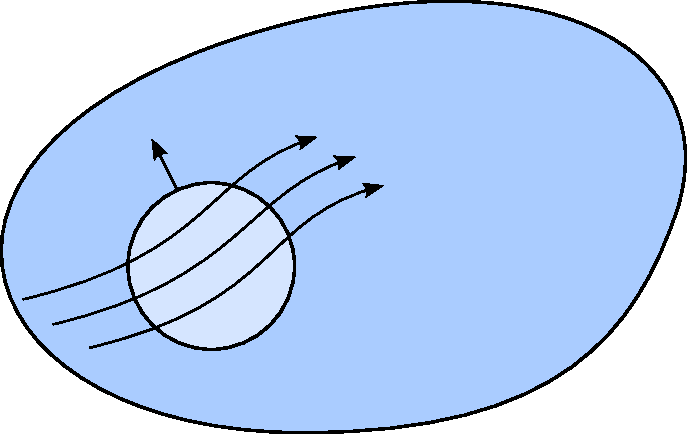
\includegraphics[width=\smallfig]{chapters/kirby-7/pdf/heat_equation_model_domain.tex}
  \fenicsfig{kirby-7}{heat_equation_model_domain}{\smallfig}
  \caption{Poisson's equation is a simple consequence of balance of
    energy in an arbitrary test volume~$\omega \subset \Omega$.}
\end{figure}

%------------------------------------------------------------------------------
\section{Finite element discretization}
\index{finite element discretization}

\subsection{Discretizing Poisson's equation}

To discretize Poisson's equation~(\ref{eq:poisson}) by the finite
element method, we first multiply by a test function $v$ and integrate
by parts to obtain
\begin{equation}
  \int_{\Omega} \nabla u \cdot \nabla v \dx
  - \int_{\partial \Omega} \partial_n u \, v \ds
  =
  \int_{\Omega} f v \dx.
\end{equation}
Letting the test function~$v$ vanish on the Dirichlet boundary
$\Gamma_{\mathrm{D}}$ where the solution $u$ is known, we arrive at
the following classical variational problem: find $u \in V$ such that
\begin{equation} \label{eq:poisson,varproblem}
  \int_{\Omega} \nabla u \cdot \nabla v \dx =
  \int_{\Omega} f v \dx - \int_{\Gamma_{\mathrm{N}}} g v \ds
  \quad \foralls v \in \hat{V}.
\end{equation}
The test space $\hat{V}$ is defined by
\begin{equation}
  \hat{V} = \{v \in H^1(\Omega) : v = 0 \mbox{ on } \Gamma_{\mathrm{D}}\},
\end{equation}
and the trial space \( V \) contains members of \( \hat{V} \) shifted
by the Dirichlet condition:
\begin{equation}
  V = \{ v \in H^1(\Omega) : v = u_0 \mbox{ on } \Gamma_{\mathrm{D}} \}.
\end{equation}

We may now discretize Poisson's equation by restricting the
variational problem~(\ref{eq:poisson,varproblem}) to a pair of
discrete spaces: find $u_h \in V_h \subset V$ such that
\begin{equation} \label{eq:poisson,varproblem,discrete}
  \int_{\Omega} \nabla u_h \cdot \nabla v \dx =
  \int_{\Omega} f v \dx - \int_{\Gamma_{\mathrm{N}}} g v \ds
  \quad \foralls v \in \hat{V}_h \subset \hat{V}.
\end{equation}
We note here that the Dirichlet condition $u = u_0$ on
$\Gamma_{\mathrm{D}}$ enters directly into the definition of the trial
space~$V_h$ (it is an \emph{essential} boundary condition), whereas
the Neumann condition $-\partial_n u = g$ on $\Gamma_{\mathrm{N}}$
enters into the variational problem (it is a \emph{natural} boundary
condition).

To solve the discrete variational
problem~(\ref{eq:poisson,varproblem,discrete}), we must construct a
suitable pair of discrete trial and test spaces $V_h$ and $\hat{V}_h$.
We return to this issue below, but assume for now that we have a basis
$\{\phi_j\}_{j=1}^N$ for $V_h$ and a basis $\{\hat{\phi}_i\}_{i=1}^N$
for $\hat{V}_h$. Here, $N$ denotes the dimension of the spaces~$V_h$ and $\hat{V}_h$.
We may then make an Ansatz for $u_h$ in terms of the basis functions
of the trial space,
%
\index{finite element solution}
\index{finite element space}
%
\begin{equation}
  u_h(x) = \sum_{j=1}^N U_j \phi_j(x),
\end{equation}
where $U \in \R^N$ is the vector of degrees of freedom to be computed.
Inserting this into~(\ref{eq:poisson,varproblem,discrete}) and varying
the test function $v$ over the basis functions of the discrete test
space $\hat{V}_h$, we obtain
\begin{equation}
  \sum_{j=1}^N U_j \int_{\Omega} \nabla \phi_j \cdot \nabla \hat{\phi}_i \dx =
  \int_{\Omega} f \hat{\phi}_i \dx - \int_{\Gamma_{\mathrm{N}}} g \hat{\phi}_i \ds,
  \quad i = 1,2,\ldots,N.
\end{equation}
We may thus compute the finite element solution $u_h = \sum_{j=1}^N
U_j \phi_j$ by solving the linear system
\begin{equation}
  AU = b,
\end{equation}
where
\begin{equation}
\begin{split}
  A_{ij} &= \int_{\Omega} \nabla \phi_j \cdot \nabla \hat{\phi}_i \dx,
  \\
  b_i &= \int_{\Omega} f \hat{\phi}_i \dx - \int_{\Gamma_{\mathrm{N}}} g \hat{\phi}_i \ds.
\end{split}
\end{equation}

\subsection{Discretizing the first-order system}
\label{sec:kirby-7:mixed}
\index{mixed problem}

We may similarly discretize the first-order
system~(\ref{eq:poisson,mixed}) by multiplying the first equation by a
test function $v$ and the second equation by a test function
$\tau$. Summing up and integrating by parts, we find that
\begin{equation}
  \int_{\Omega} (\nabla \cdot \sigma) \, v + \sigma \cdot \tau
  - u \nabla \cdot \tau \dx +
  \int_{\partial\Omega} u \tau \cdot n \ds
  = \int_{\Omega} f v \dx
  \quad \foralls (v, \tau) \in \hat{V}.
\end{equation}
The normal flux $\sigma \cdot n = g$ is known on the Neumann
boundary~$\Gamma_{\mathrm{N}}$ so we may take $\tau \cdot n = 0$
on~$\Gamma_{\mathrm{N}}$.  Inserting the value for $u$ on the
Dirichlet boundary~$\Gamma_{\mathrm{D}}$, we arrive at the following
variational problem: find $(u, \sigma) \in V$ such that
\begin{equation} \label{eq:poisson,varproblem,mixed}
  \int_{\Omega} (\nabla \cdot \sigma) \, v + \sigma \cdot \tau
  - u \nabla \cdot \tau \dx
  = \int_{\Omega} f v \dx - \int_{\Gamma_{\mathrm{D}}} u_0 \tau \cdot n \ds
  \quad \foralls (v, \tau) \in \hat{V}.
\end{equation}
A suitable choice of trial and test spaces is
\begin{equation}
  \begin{split}
    V       &= \{(v, \tau) : v \in L^2(\Omega), \tau \in H(\mathrm{div}, \Omega), \tau \cdot n = g \mbox{ on } \Gamma_{\mathrm{N}}\},
    \\
    \hat{V} &= \{(v, \tau) : v \in L^2(\Omega), \tau \in H(\mathrm{div}, \Omega), \tau \cdot n = 0 \mbox{ on } \Gamma_{\mathrm{N}}\}.
  \end{split}
\end{equation}
Note that the variational problem~(\ref{eq:poisson,varproblem,mixed})
differs from the variational problem~(\ref{eq:poisson,varproblem}) in
that the Dirichlet condition $u = u_0$ on $\Gamma_{\mathrm{D}}$ enters
into the variational formulation (it is now a natural boundary
condition), whereas the Neumann condition $\sigma \cdot n = g$ on
$\Gamma_{\mathrm{N}}$ enters into the definition of the trial space
$V$ (it is now an essential boundary condition).

As above, we restrict the variational problem to a pair of discrete
trial and test spaces $V_h \subset V$ and $\hat{V}_h \subset \hat{V}$
and make an Ansatz for the finite element solution of the form
\begin{equation}
  (u_h, \sigma_h) = \sum_{j=1}^N U_j (\phi_j, \psi_j),
\end{equation}
where $\{(\phi_j, \psi_j)\}_{j=1}^N$ is a basis for the trial space
$V_h$. Typically, either \( \phi_j \) or \( \psi_j \) will vanish, so
that the basis is really the tensor product of a basis for the \( L^2
\) space with a basis for the \( H(\mathrm{div}) \) space. We thus
obtain a linear system for the degrees of freedom $U \in \R^N$ by
solving a linear system $A U = b$, where now
\begin{equation} \label{eq:mixedsystem}
  \begin{split}
    A_{ij} &=
    \int_{\Omega} (\nabla \cdot \psi_j) \, \hat{\phi}_i
    + \psi_j \cdot \hat{\psi}_i
    - \phi_j \nabla \cdot \hat{\psi}_i \dx,
    \\
    b_i &=
    \int_{\Omega} f \hat{\phi}_i \dx
    - \int_{\Gamma_{\mathrm{D}}} u_0 \, \hat{\psi}_i \cdot n \ds.
  \end{split}
\end{equation}

\index{Ladyzhenskaya--\babuska{}--Brezzi conditions}
\index{LBB conditions}
The finite element discretization~\eqref{eq:mixedsystem} is an example
of a \emph{mixed method}. Such formulations require some care in
selecting spaces that discretize the different function spaces, here
$L^2$ and $H(\mathrm{div})$, in a compatible way.  Stable
discretizations must satisfy the so-called \emph{inf--sup} or
Ladyzhenskaya--\babuska{}--Brezzi (LBB) condition(s). This theory
explains why many of the finite element spaces for mixed methods seem
complicated compared to those for standard methods. In
Chapter~\ref{chap:kirby-6} below, we give several examples of such
finite element spaces.

%------------------------------------------------------------------------------
\section{Finite element abstract formalism}
\label{sec:abstract}

\subsection{Linear problems}
\label{sec:abstract,linear}
\index{bilinear form}
\index{linear form}

We saw above that the finite element solution of Poisson's
equation~(\ref{eq:poisson}) or~(\ref{eq:poisson,mixed}) can be
obtained by restricting an infinite-dimensional (continuous) variational problem to
a finite-dimensional (discrete) variational problem and solving a linear system.

To formalize this, we consider a general linear variational problem
written in the following canonical form: find $u \in V$ such that
\begin{equation} \label{eq:varproblem}
  a(u, v) = L(v) \quad \foralls v \in \hat{V},
\end{equation}
where $V$ is the trial space and $\hat{V}$ is the test space. We thus
express the variational problem in terms of a \emph{bilinear form}~$a$
and a \emph{linear form} (functional)~$L$:
\begin{equation}
  \begin{split}
    a &: V \times \hat{V} \rightarrow \R,
    \\
    L &: \hat{V} \rightarrow \R.
  \end{split}
\end{equation}
As above, we discretize the variational problem~(\ref{eq:varproblem})
by restricting to a pair of discrete trial and test spaces: find $u_h
\in V_h \subset V$ such that
\begin{equation} \label{eq:varproblem,discrete}
  a(u_h, v) = L(v) \quad \foralls v \in \hat{V}_h \subset \hat{V}.
\end{equation}
To solve the discrete variational
problem~(\ref{eq:varproblem,discrete}), we make an Ansatz of the form
\begin{equation} \label{eq:ansatz}
  u_h = \sum_{j=1}^N U_j \phi_j,
\end{equation}
and take $v = \hat{\phi}_i$ for $i = 1,2,\ldots,N$. As before,
$\{\phi_j\}_{j=1}^N$ is a basis for the discrete trial space~$V_h$ and
$\{\hat{\phi}_i\}_{i=1}^N$ is a basis for the discrete test
space~$\hat{V}_h$. It follows that
\begin{equation}
  \sum_{j=1}^N U_j \, a(\phi_j, \hat{\phi}_i) = L(\hat{\phi}_i), \quad i
  = 1,2,\ldots,N.
\end{equation}
The degrees of freedom~$U$ of the finite element solution~$u_h$ may
then be computed by solving a linear system $AU = b$, where
\begin{equation} \label{eq:system}
  \begin{split}
    A_{ij} &= a(\phi_j, \hat{\phi}_i), \quad i, j = 1,2,\ldots,N, \\
    b_i &= L(\hat{\phi}_i).
  \end{split}
\end{equation}

\subsection{Nonlinear problems}
\label{sec:abstract,nonlinear}
\index{nonlinear problems}

We also consider nonlinear variational problems written in the
following canonical form: find $u \in V$ such that
\begin{equation} \label{eq:varproblem,nonlinear}
  F(u; v) = 0 \quad \foralls v \in \hat{V},
\end{equation}
where now~$F : V \times \hat{V} \rightarrow \R$ is a \emph{semilinear}
form, linear in the argument(s) subsequent to the semicolon. As above,
we discretize the variational problem~(\ref{eq:varproblem,nonlinear})
by restricting to a pair of discrete trial and test spaces: find $u_h
\in V_h \subset V$ such that
\begin{equation}
  F(u_h; v) = 0 \quad \foralls v \in \hat{V}_h \subset \hat{V}.
\end{equation}
The finite element solution $u_h = \sum_{j=1}^N U_j \phi_j$ may then
be computed by solving a nonlinear system of equations,
\begin{equation} \label{eq:system,nonlinear}
  b(U) = 0,
\end{equation}
where $b : \R^N \rightarrow \R^N$ and
\begin{equation}
  b_i(U) = F(u_h; \hat{\phi}_i), \quad i=1,2,\ldots,N.
\end{equation}

\index{Newton's method}
\index{linearization}
%
To solve the nonlinear system~(\ref{eq:system,nonlinear}) by Newton's
method or some variant of Newton's method, we compute the Jacobian $A
= b'$. We note that if the semilinear form~$F$ is differentiable
in~$u$, then the entries of the Jacobian~$A$ are given by
\begin{equation} \label{eq:jacobian}
    A_{ij}(u_h)
    = \frac{\partial b_i(U)}{\partial U_j}
    = \frac{\partial}{\partial U_j} F(u_h; \hat{\phi}_i)
    = F'(u_h; \hat{\phi}_i) \, \frac{\partial u_h}{\partial U_j}
    = F'(u_h; \hat{\phi}_i) \, \phi_j
    \equiv F'(u_h; \phi_j, \hat{\phi}_i).
\end{equation}
In each Newton iteration, we must then evaluate (assemble) the matrix
$A$ and the vector $b$, and update the solution vector~$U$ by
\begin{equation}
  U^{k+1} = U^k - \delta U^k, \quad k = 0,1,\ldots,
\end{equation}
where $\delta U^k$ solves the linear system
\begin{equation} \label{eq:system,linearization}
  A(u_h^k) \, \delta U^k = b(u_h^k).
\end{equation}

We note that for each fixed $u_h$, $a = F'(u_h; \cdot, \cdot)$ is a
bilinear form and $L = F(u_h; \cdot)$ is a linear form. In each Newton
iteration, we thus solve a linear variational problem of the canonical
form~(\ref{eq:varproblem}): find $\delta u \in V_{h,0}$ such that
\begin{equation} \label{eq:varproblem,newton}
    F'(u_h; \delta u, v) = F(u_h; v) \quad \foralls v \in \hat{V}_h,
\end{equation}
where $V_{h,0} = \{v - w: v, w \in
V_h\}$. Discretizing~(\ref{eq:varproblem,newton}) as in
Section~\ref{sec:abstract,linear}, we recover the linear
system~(\ref{eq:system,linearization}).

\begin{example}[Nonlinear Poisson equation]
\index{nonlinear Poisson equation}

As an example, consider the following nonlinear Poisson equation:
\begin{equation} \label{eq:poisson,nonlinear}
  \begin{split}
    - \nabla \cdot ((1+u) \nabla u) &= f \quad \mbox{ in } \Omega,
    \\
    u &= 0 \quad \mbox{ on } \partial\Omega.
  \end{split}
\end{equation}
Multiplying (\ref{eq:poisson,nonlinear}) with a test function~$v$ and
integrating by parts, we obtain
\begin{equation}
  \int_{\Omega} ((1+u) \nabla u) \cdot \nabla v \dx =
  \int_{\Omega} f v \dx,
\end{equation}
which is a nonlinear variational problem of the
form~(\ref{eq:varproblem,nonlinear}), with
\begin{equation}
  F(u; v) = \int_{\Omega} ((1+u) \nabla u) \cdot \nabla v \dx
  - \int_{\Omega} f v \dx.
\end{equation}
Linearizing the semilinear form~$F$ around $u = u_h$, we obtain
\begin{equation}
  F'(u_h; \delta u, v) =
  \int_{\Omega} (\delta u \nabla u_h) \cdot \nabla v \dx +
  \int_{\Omega} ((1 + u_h) \nabla \delta u) \cdot \nabla v \dx.
\end{equation}
We may thus compute the entries of the Jacobian matrix~$A(u_h)$ by
\begin{equation}
  A_{ij}(u_h) = F'(u_h; \phi_j, \hat{\phi}_i) =
  \int_{\Omega} (\phi_j \nabla u_h) \cdot \nabla \hat{\phi}_i \dx +
  \int_{\Omega} ((1 + u_h) \nabla \phi_j) \cdot \nabla \hat{\phi}_i \dx.
\end{equation}

\end{example}

%------------------------------------------------------------------------------
\section{Finite element function spaces}
\index{finite element function spaces}

In the above discussion, we assumed that we could construct discrete
subspaces $V_h \subset V$ of infinite-dimensional function spaces. A
central aspect of the finite element method is the construction of
such subspaces by patching together local function spaces defined by a
set of \emph{finite elements}. We here give a general overview of the
construction of finite element function spaces and return in
Chapters~\ref{chap:kirby-6} and~\ref{chap:kirby-1} to the construction
of specific function spaces as subsets of $H^1$, $H(\mathrm{curl})$,
$H(\mathrm{div})$ and $L^2$.

\subsection{The mesh}
\index{mesh}

To define $V_h$, we first partition the domain~$\Omega$ into a finite
set of cells $\mesh = \{T\}$ with disjoint interiors such that\vspace*{4pt}
\begin{equation}
  \cup_{T\in\mesh} T = \Omega.\vspace*{4pt}
\end{equation}
Together, these cells form a \emph{mesh} of the domain~$\Omega$. The
cells are typically simple polygonal shapes like intervals, triangles,
quadrilaterals, tetrahedra or hexahedra as shown in
Figure~\ref{fig:shapes}. But other shapes are possible, in particular
curved cells to capture the boundary of a non-polygonal domain
correctly.
% as shown in Figure~\ref{fig:shapes,curved}.

\begin{figure}
\bwfig
  \ffigbox{\caption{Examples of finite element cells in one, two and three
           space dimensions.}\label{fig:shapes}}
  {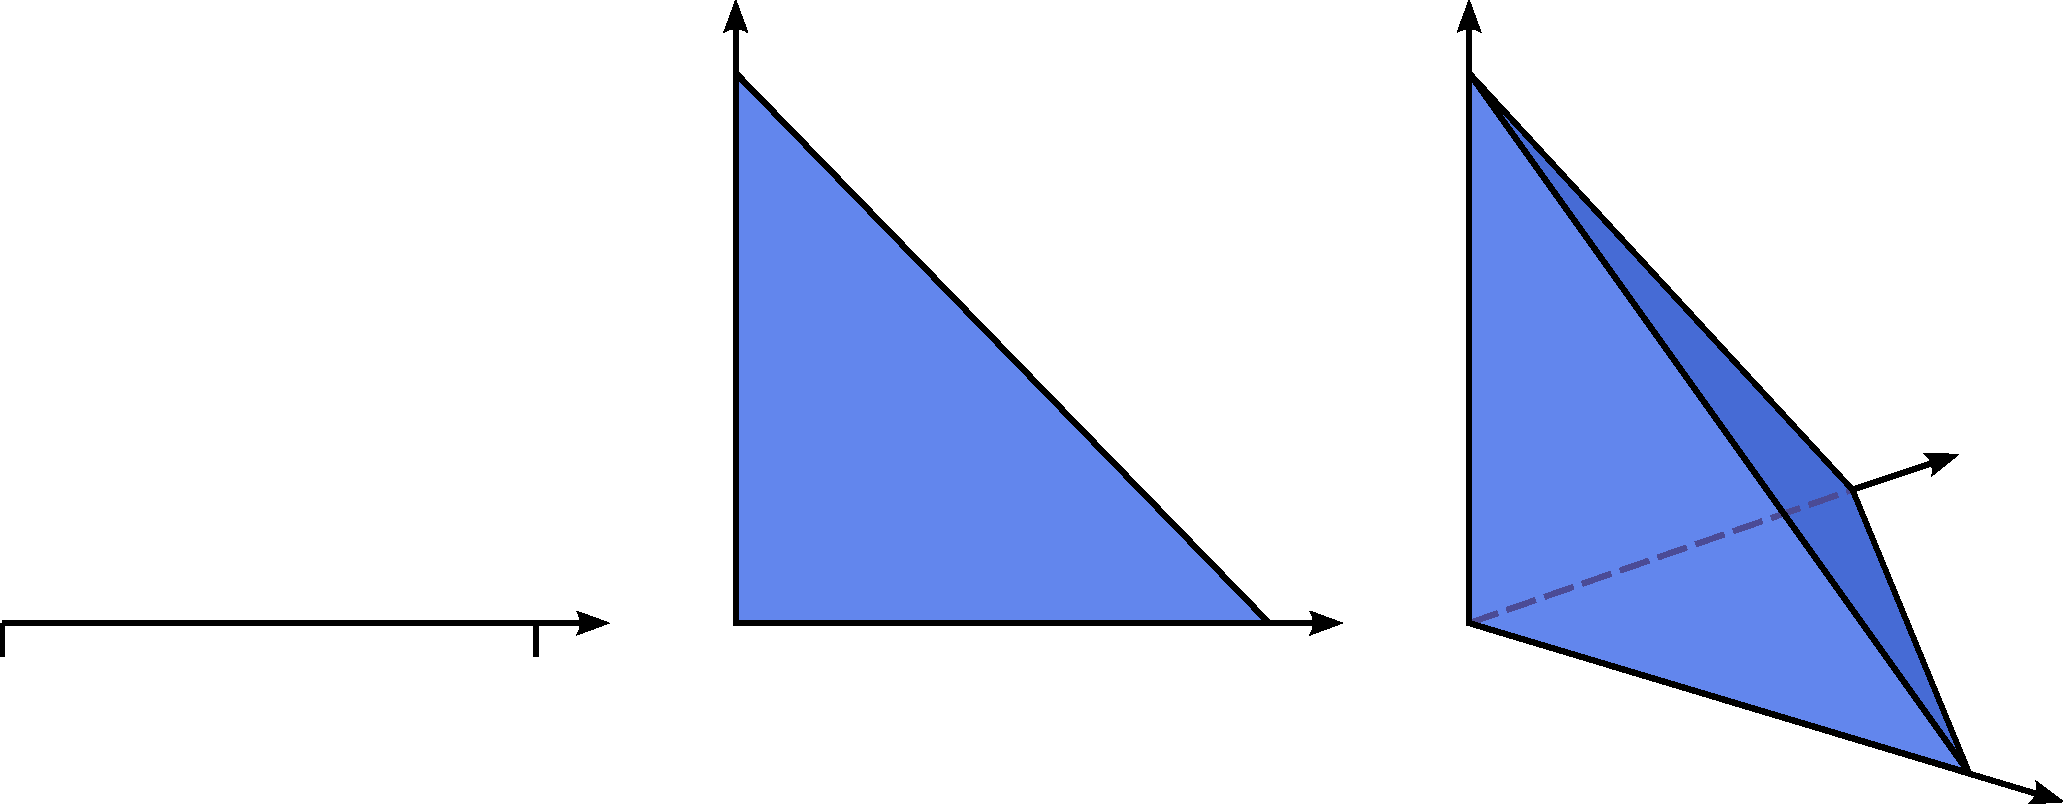
\includegraphics[width=\largefig]{chapters/kirby-7/pdf/cells.pdf}}
\end{figure}

%\begin{figure}
%  \caption{A straight triangular cell (left) and curved triangular
%      cell (right).}
%  \label{fig:shapes,curved}}
%  \includegraphics[width=\largefig,height=3cm]{chapters/kirby-7/pdf/straight_and_cur%ved_triangles.pdf}
%\end{figure}

\enlargethispage{-5pt}
\vspace*{4pt}
\subsection{The finite element definition}

Once a domain~$\Omega$ has been partitioned into cells, one may define
a local function space $\CiarletSpace$ on each cell $T$ and use these
local function spaces to build the global function space~$V_h$. A cell
$T$ together with a local function space $\CiarletSpace$ and a set of
rules for describing the functions in $\CiarletSpace$ is called a
\emph{finite element}. This definition was first
formalized by~\citet{Ciarlet1976} and it remains the standard
formulation today~\citep{BrennerScott2008}. The formal definition
reads as follows: a finite element is a triple $(T,
\CiarletSpace, \mathcal{L})$, where
\femdefinition{}

As an example, consider the standard linear Lagrange finite element on
the triangle in~Figure~\ref{fig:P1}. The cell~$T$ is given by the
triangle and the space $\CiarletSpace$ is given by the space of first
degree polynomials on $T$ (a space of dimension three). As a basis for
$\CiarletSpace'$, we may take point evaluation at the three vertices
of $T$; that is,
\begin{equation}
  \begin{split}
    \ell_i : \CiarletSpace \rightarrow \R,
    \\
    \ell_i(v) = v(x^i),
  \end{split}
\end{equation}
\looseness-1{}for $i=1,2,3$ where $x^i$ is the coordinate of the $i$th vertex. To
check that this is indeed a finite element, we need to verify that
$\mathcal{L}$ is a basis for $\CiarletSpace'$. This is equivalent to
the unisolvence of $\mathcal{L}$; that is, if $v\in\CiarletSpace$ and
$\ell_i(v) = 0$ for all $\ell_i$, then $v =
0$~\citep{BrennerScott2008}. For the linear Lagrange triangle, we note
that if $v$ is zero at each vertex, then $v$ must be zero everywhere,
since a plane is uniquely~determined by its values at three
non-collinear points. It follows that the linear Lagrange triangle is
indeed a finite element. In general, determining the unisolvence of
$\mathcal{L}$ may be non-trivial.

\begin{figure}
\bwfig
  \centering
  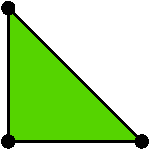
\includegraphics[width=\smallfig]{chapters/kirby-7/pdf/P1.pdf}
  \caption{The degrees of freedom of the linear Lagrange (Courant)
    triangle are given by point evaluation at the three vertices of
    the triangle.}
  \label{fig:P1}
\end{figure}

\subsection{The nodal basis}
\index{nodal basis}

Expressing finite element solutions in $V_h$ in terms of basis
functions for the local function spaces $\CiarletSpace$ may be greatly
simplified by introducing a \emph{nodal basis} for $\CiarletSpace$.  A
nodal basis $\{\phi_i\}_{i=1}^{n}$ for~$\CiarletSpace$ is a basis for
$\CiarletSpace$ that satisfies
\begin{equation} \label{eq:nodalbasis}
  \ell_i(\phi_j) = \delta_{ij}, \quad i, j = 1,2,\ldots, n.
\end{equation}
It follows that any $v \in \CiarletSpace$ may be expressed by
\begin{equation}
  v = \sum_{i=1}^{n} \ell_i(v) \phi_i.
\end{equation}
In particular, any function $v$ in $\CiarletSpace$ for the linear
Lagrange triangle is given by $v = \sum_{i=1}^3 v(x^i) \phi_i$. In
other words, the expansion coefficients of any function $v$ may be
obtained by evaluating the linear functionals in~$\mathcal{L}$
at~$v$. We shall therefore interchangeably refer to both the expansion
coefficients~$U$ of $u_h$ and the linear functionals of $\mathcal{L}$
as the \emph{degrees of freedom}.
\index{linear Lagrange element}

\begin{example}[Nodal basis for the linear Lagrange simplices]
  The nodal basis for the linear Lagrange interval with vertices at
  $x^1 = 0$ and $x^2 = 1$ is given by
  \begin{equation}
    \phi_1(x) = 1 - x, \quad
    \phi_2(x) = x.
  \end{equation}
  The nodal basis for the linear Lagrange triangle with vertices at
  $x^1 = (0, 0)$, $x^2 = (1, 0)$ and $x^3 = (0, 1)$ is given by
  \begin{equation}
    \phi_1(x) = 1 - x_1 - x_2, \quad
    \phi_2(x) = x_1, \quad
    \phi_3(x) = x_2.
  \end{equation}
  The nodal basis for the linear Lagrange tetrahedron with vertices at
  $x^1 = (0, 0, 0)$, $x^2 = (1, 0, 0)$, $x^3 = (0, 1, 0)$ and $x^4 =
  (0, 0, 1)$ is given by
  \begin{equation}
    \begin{array}{cc}
      \begin{array}{rcl}
        \phi_1(x) &=& 1 - x_1 - x_2 - x_3, \\
        \phi_3(x) &=& x_2,
      \end{array}
      &
      \begin{array}{rcl}
        \phi_2(x) &=& x_1, \\
        \phi_4(x) &=& x_3.
      \end{array}
    \end{array}
  \end{equation}
\end{example}

For any finite element $(T, \CiarletSpace, \mathcal{L})$, the nodal
basis may be computed by solving a linear system of size $n \times
n$. To see this, let $\{\psi_i\}_{i=1}^{n}$ be any basis (the
\emph{prime} basis) for $\CiarletSpace$. Such a basis is easy to
construct if $\CiarletSpace$ is a full polynomial space or may
otherwise be computed by a singular-value decomposition or a
Gram--Schmidt procedure; see~\citet{Kirby2004}. We may then make an
Ansatz for the nodal basis in terms of the prime basis:
\begin{equation}
  \phi_j = \sum_{k=1}^{n} \alpha_{jk} \psi_k, \quad j = 1,2,\ldots,n.
\end{equation}
Inserting this into~(\ref{eq:nodalbasis}), we find that
\begin{equation}
  \sum_{k=1}^{n} \alpha_{jk} \ell_i(\psi_k) = \delta_{ij}, \quad i, j = 1,2,\ldots,n.
\end{equation}
In other words, the coefficients~$\alpha$ expanding the nodal basis
functions in the prime basis may be computed by solving the linear
system
\begin{equation}
  B \alpha^{\top} = I,
\end{equation}
where $B_{ij} = \ell_i(\psi_j)$.

\subsection{The local-to-global mapping}
\index{local-to-global mapping}

Now, to define a global function space $V_h = \mathrm{span}
\{\phi_i\}_{i=1}^N$ on $\Omega$ from a given set $\{(T,
\CiarletSpace_T,\mathcal{L}_T)\}_{T\in\mesh}$ of finite elements, we
also need to specify how the local function spaces are patched
together. We do this by specifying for each cell $T \in \mesh$ a
\emph{local-to-global mapping}:
\begin{equation}
  \iota_T : [1, n_T] \rightarrow [1, N].
\end{equation}
This mapping specifies how the local degrees of freedom~$\mathcal{L}_T =
\{\ell_i^T\}_{i=1}^{n_T}$ are mapped to global degrees of
freedom~$\mathcal{L} = \{\ell_i\}_{i=1}^N$. More precisely, the global
degrees of freedom are defined by
\begin{equation} \label{eq:nodemapping}
  \ell_{\iota_T(i)}(v) = \ell^T_i(v|_T), \quad i = 1,2,\ldots,n_T,
\end{equation}
for any $v\in V_h$. Thus, each local degree of freedom~$\ell^T_i \in
\mathcal{L}_T$ corresponds to a global degree of
freedom~$\ell_{\iota_T(i)} \in \mathcal{L}$ determined by the
local-to-global mapping $\iota_T$. As we shall see, the
local-to-global mapping together with the choice of degrees of freedom
determine the continuity of the global function space~$V_h$.

For standard continuous piecewise linears, one may define the
local-to-global mapping by simply mapping each local vertex number $i$
for $i=1,2,3$ to the corresponding global vertex number
$\iota_T(i)$. For continuous piecewise quadratics, one can base the
local-to-global mapping on global vertex and edge numbers as
illustrated in Figure~\ref{fig:dofmap} for a simple mesh consisting of
two triangles.

\begin{figure}
\bwfig
  \centering
  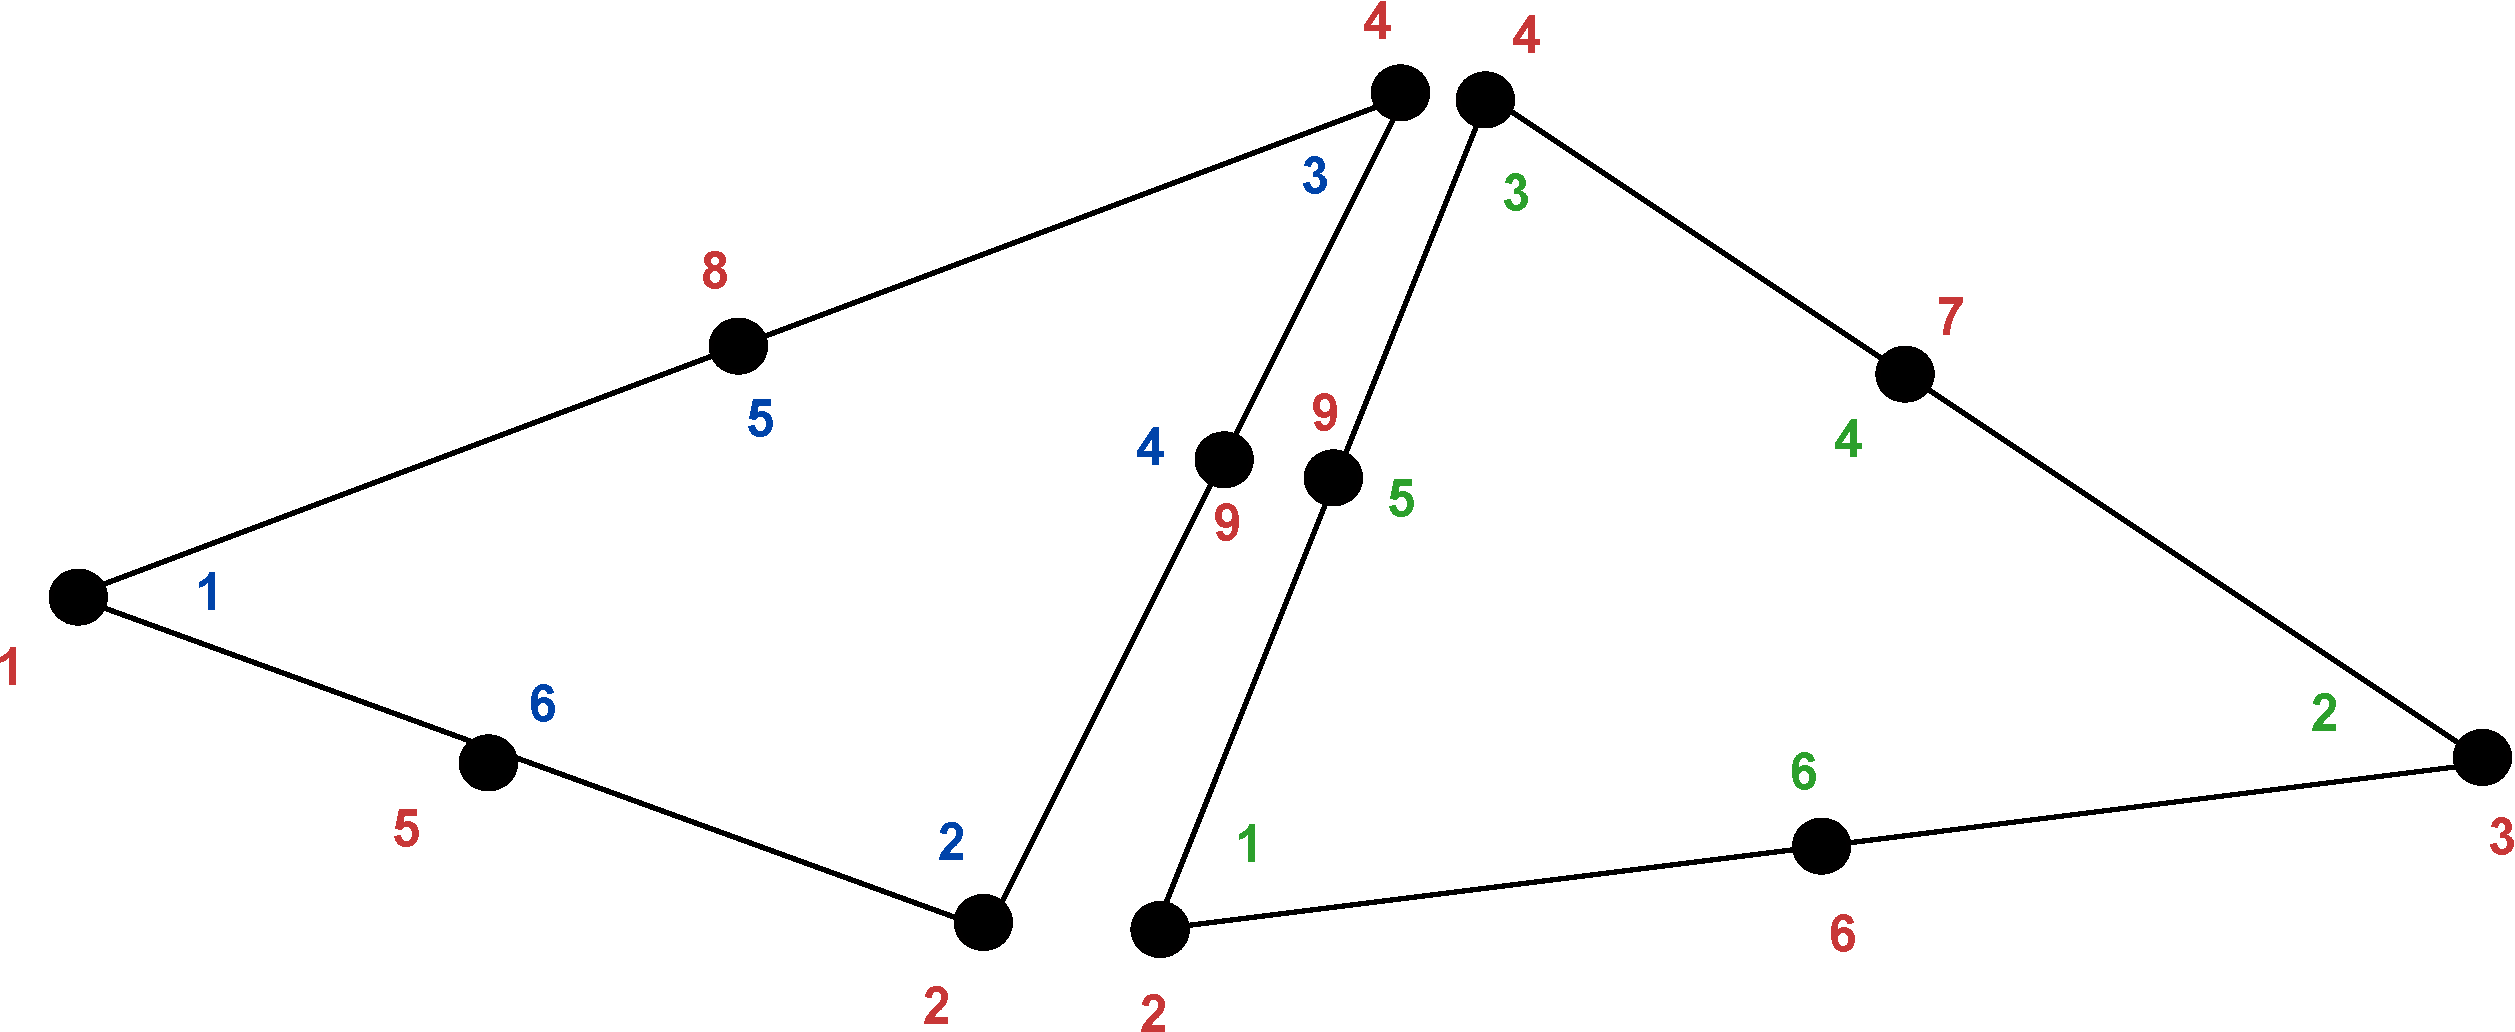
\includegraphics[width=\largefig]{chapters/kirby-7/pdf/dofmap.pdf}
  \caption{Local-to-global mapping for a simple mesh consisting of
    two triangles. The six local degrees of freedom of the left
    triangle ($T$) are mapped to the global degrees of freedom
    $\iota_T(i) = 1, 2, 4, 9, 8, 5$ for $i = 1, 2, \ldots, 6$, and
    the six local degrees of freedom of the right triangle ($T'$)
    are mapped to $\iota_{T'}(i) = 2, 3, 4, 7, 9, 6$ for $i = 1, 2,
    \ldots, 6$.}
  \label{fig:dofmap}
\end{figure}

\subsection{The global function space}
One may now define the global function space $V_h$ as the set of
functions on $\Omega$ satisfying the following pair of conditions. We
first require that
\begin{equation}
  v |_T \in \CiarletSpace_T \quad \foralls T \in \mesh;
\end{equation}
that is, the restriction of $v$ to each cell~$T$ lies in the local
function space~$\CiarletSpace_T$. Second, we require that for any pair
of cells $(T, T') \in \mesh \times \mesh$ and any pair~$(i, i') \in
[1,n_T] \times [1,n_{T'}]$ satisfying
\begin{equation}
  \iota_T(i) = \iota_{T'}(i'),
\end{equation}
it holds that
\begin{equation} \label{eq:constraint}
  \ell^T_i(v|_T) = \ell^{T'}_{i'}(v|_{T'}).
\end{equation}
In other words, if two local degrees of freedom $\ell_i^T$ and
$\ell^{T'}_{i'}$ are mapped to the same global degree of freedom, then
they must agree for each function $v \in V_h$. Here, $v|_T$ denotes
(the continuous extension of the) restriction of $v$ to the interior
of $T$. This is illustrated in Figure~\ref{fig:femspace} for the space
of continuous piecewise quadratics obtained by patching together two
quadratic Lagrange triangles.

\begin{figure}
  \centering
  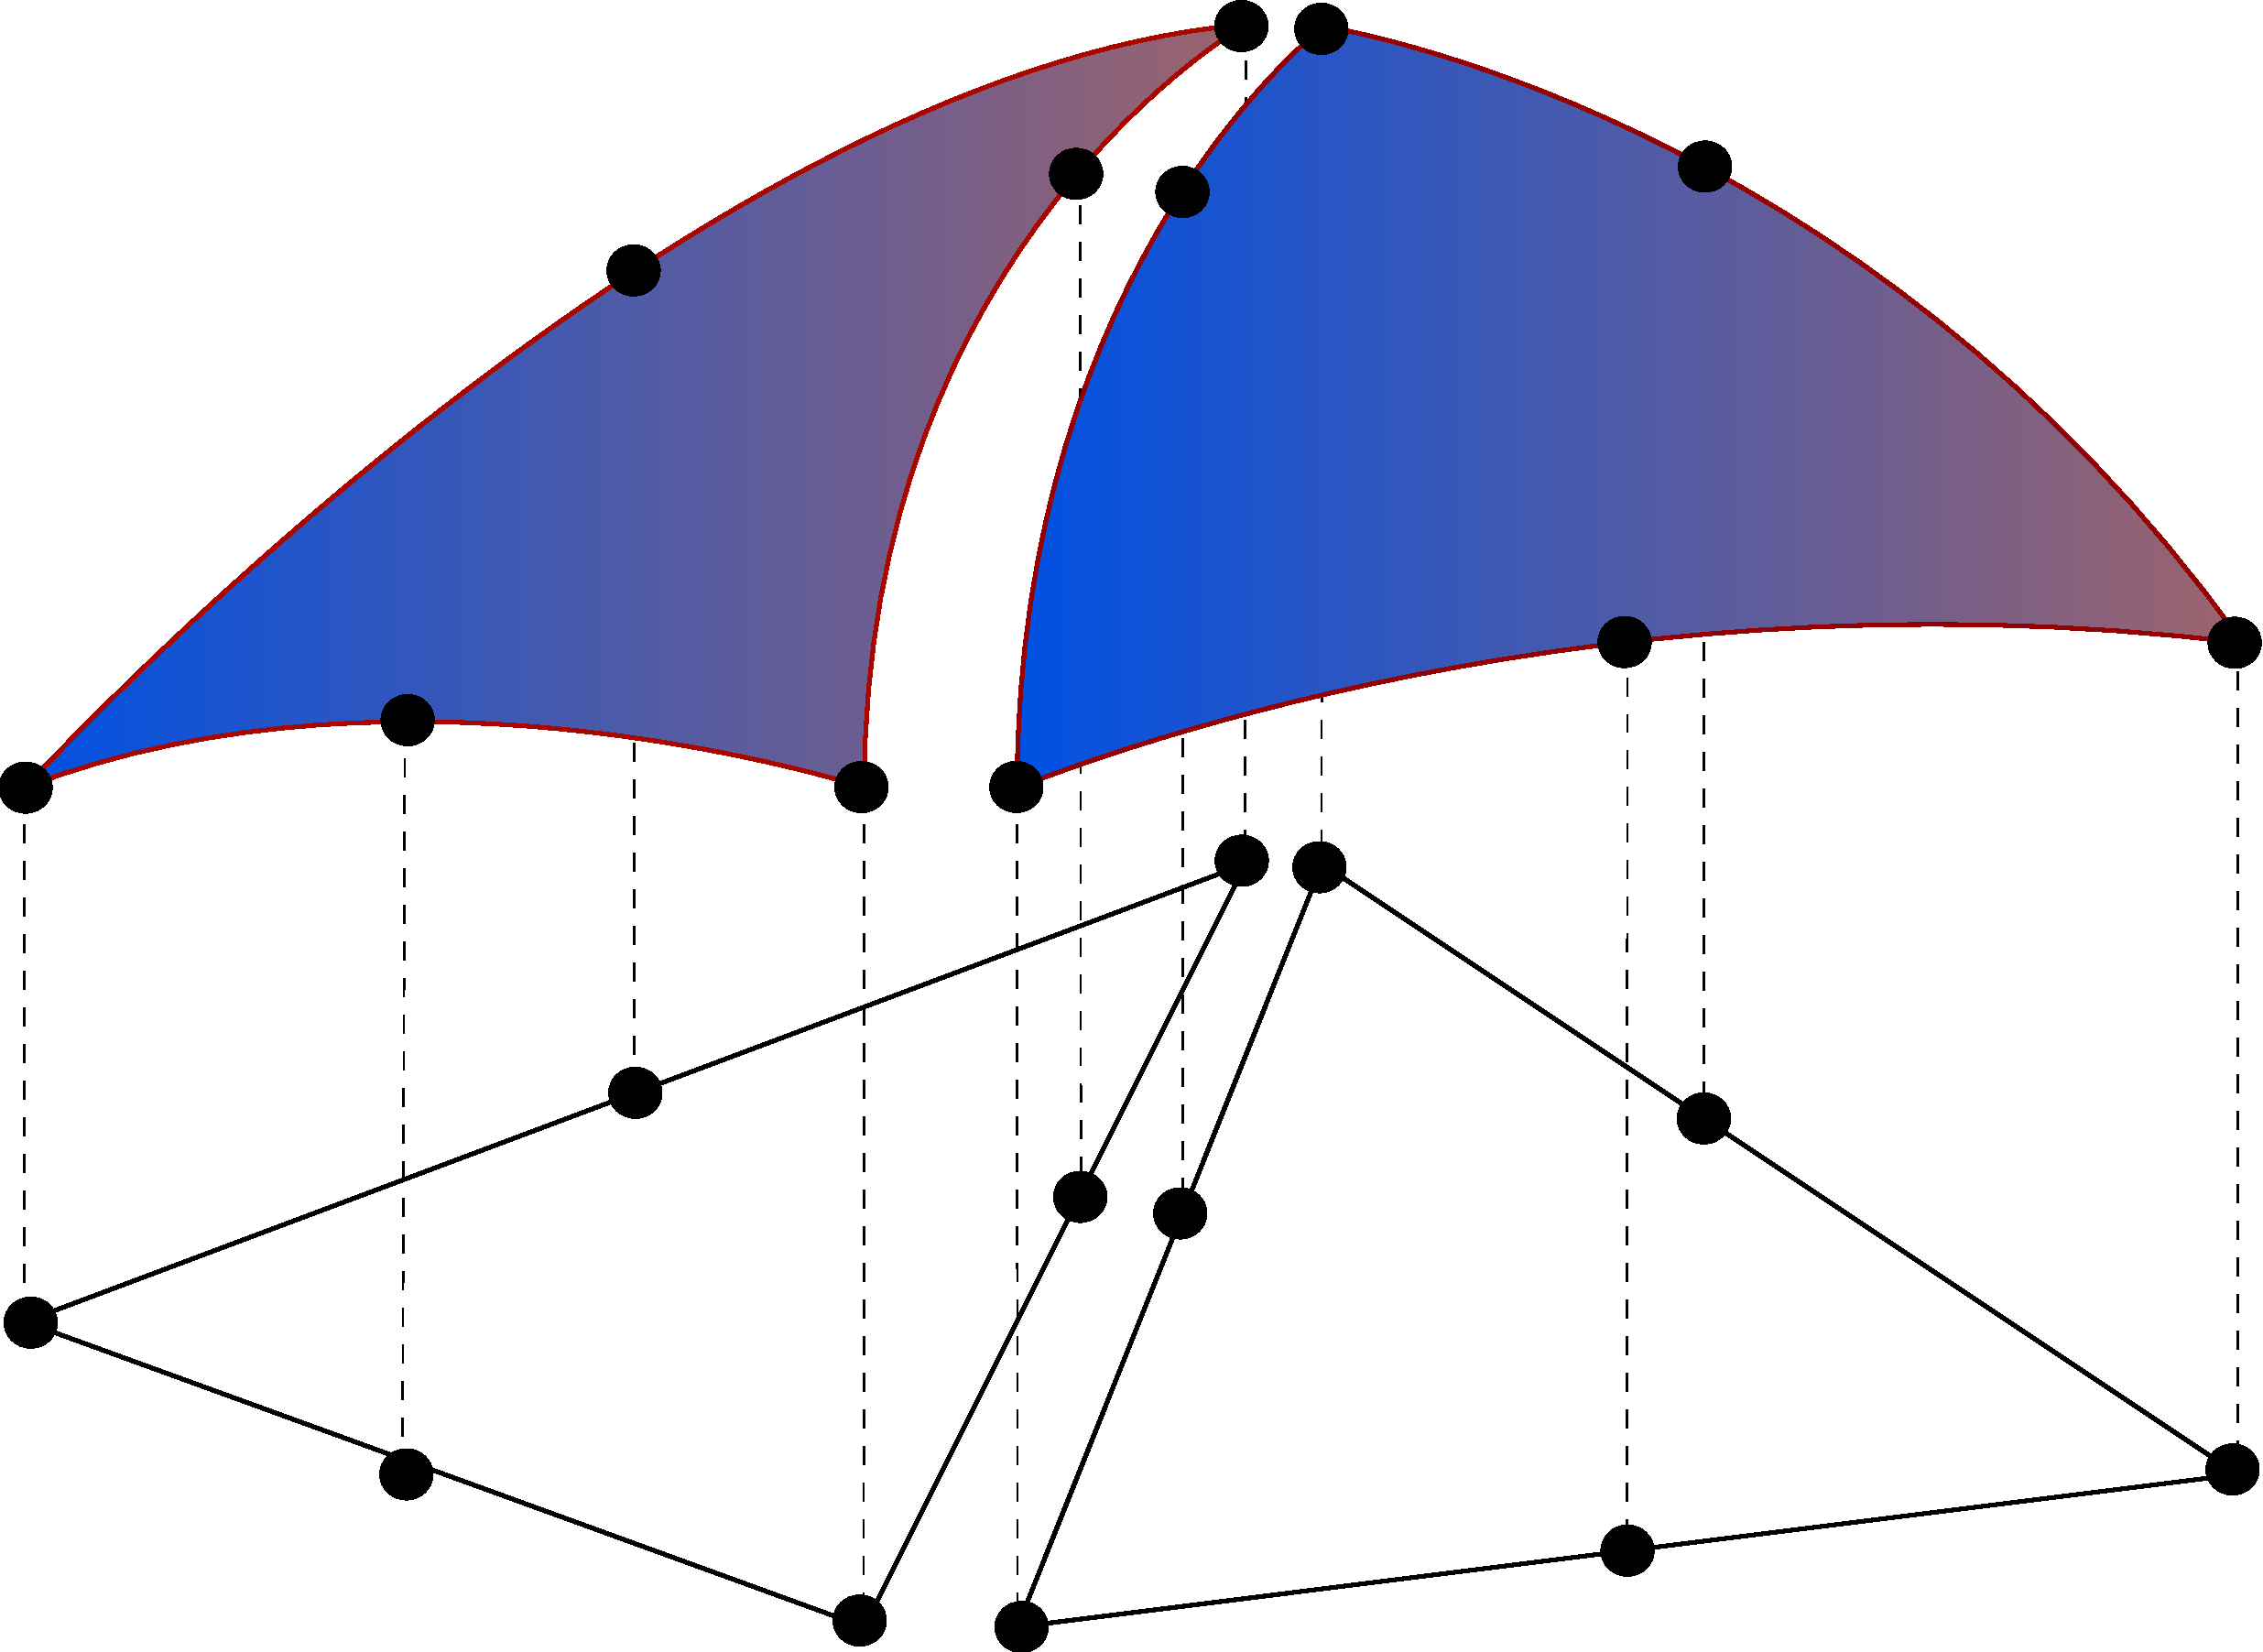
\includegraphics[width=\largefig]{chapters/kirby-7/pdf/femspace.pdf}
  \caption{Patching together a pair of quadratic local function
    spaces on a pair of cells $(T, T')$ to form a global continuous
    piecewise quadratic function space on $\Omega = T \cup T'$.}
  \label{fig:femspace}
\end{figure}

Note that by this construction, the functions in $V_h$ are undefined
on cell boundaries, unless the constraints (\ref{eq:constraint}) force
the functions in $V_h$ to be continuous on cell boundaries. However,
this is usually not a problem, since we can perform all operations on
the restrictions of functions to the local cells.

The local-to-global mapping together with the choice of degrees of
freedom determine the continuity of the global function space~$V_h$.
For the linear Lagrange triangle, choosing the degrees of freedom as
point evaluation at the vertices ensures that all functions in $V_h$
must be continuous at the two vertices of the common edge of any pair
of adjacent triangles, and therefore along the entire common edge. It
follows that the functions in $V_h$ are continuous throughout the
domain~$\Omega$. As a consequence, the space of piecewise linears
generated by the Lagrange triangle is $H^1$-conforming; that is, $V_h
\subset H^1(\Omega)$.

\index{Crouzeix--Raviart element}
\index{Brezzi--Douglas--Marini element}
\index{\nedelec{} element}
%
One may also consider degrees of freedom defined by point evaluation
at the midpoint of each edge. This is the so-called Crouzeix--Raviart
triangle. The corresponding global Crouzeix--Raviart space $V_h$ is
consequently continuous only at edge midpoints. The Crouzeix--Raviart
triangle is an example of an $H^1$-\emph{nonconforming} element; that
is, the function space $V_h$ constructed from a set of
Crouzeix--Raviart elements is not a subspace of $H^1$. Other choices
of degrees of freedom may ensure continuity of normal components, like
for the $\Hdiv$-conforming Brezzi--Douglas--Marini elements, or
tangential components, as for the $\Hcurl$-conforming \nedelec{}
elements. In Chapter~\ref{chap:kirby-6}, other examples of elements
are given which ensure different kinds of continuity by the choice of
degrees of freedom and local-to-global mapping.

\enlargethispage{12pt}

\vspace*{-6pt}\subsection{The mapping from the reference element}
\index{mapping from reference element}
\index{affine mapping}

As we have seen, the global function space $V_h$ may be described by a
mesh $\mesh$, a set of finite elements
$\{(T,\CiarletSpace_T,\mathcal{L}_T)\}_{T\in\mesh}$ and a set of
local-to-global mappings $\{\iota_T\}_{T\in\mesh}$. We may simplify
this description further by introducing a \emph{reference finite
  element} $(\hat{T},\hat{\CiarletSpace},\hat{\mathcal{L}})$,
where $\hat{\mathcal{L}} =
\{\hat{\ell}_1,\hat{\ell}_2,\ldots,\hat{\ell}_{\hat{n}}\}$, and
a set of invertible mappings $\{F_T\}_{T\in\mesh}$ that map the
reference cell~$\hat{T}$ to the cells of the mesh:
\begin{equation}
  T = F_T(\hat{T}) \quad \foralls T \in \mesh.
\end{equation}
This is illustrated in Figure~\ref{fig:kirby-7:affinemap}. Note that
$\hat{T}$ is generally not part of the mesh.

\begin{figure}%10
\bwfig
%  \centering
%  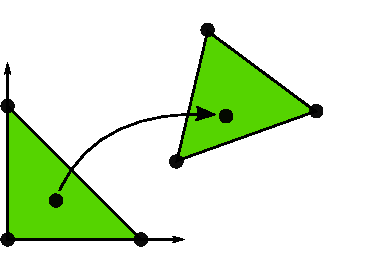
\includegraphics[width=\largefig]{chapters/kirby-7/pdf/affine_map.pdf}
  \fenicsfig{kirby-7}{affine_map}{\largefig}
  \caption{The (affine) map $F_T$ from a reference cell $\hat{T}$
    to a cell $T \in \mesh$.}
  \label{fig:kirby-7:affinemap}
\end{figure}

\index{Piola mapping}
\index{covariant Piola mapping}
\index{contravariant Piola mapping}
%
For function spaces discretizing $H^1$ as
in~(\ref{eq:poisson,varproblem}), the mapping $F_T$ is typically
\emph{affine}; that is, $F_T$ can be written in the form $F_T(\hat{x})
= A_T \hat{x} + b_T$ for some matrix $A_T \in \R^{d\times d}$ and some
vector $b_T \in \R^d$, or else \emph{isoparametric}, in which case the
components of $F_T$ are functions in $\hat{\CiarletSpace}$. For function
spaces discretizing $\Hdiv$ like
in~(\ref{eq:poisson,varproblem,mixed}) or $\Hcurl$, the appropriate
mappings are the contravariant and covariant Piola mappings which
preserve normal and tangential components, respectively;
see~\citet{RognesKirbyLogg2009}. For simplicity, we restrict the
following discussion to the case when $F_T$ is affine or
isoparametric.

For each cell $T \in \mesh$, the mapping $F_T$ generates a
function space on $T$ given by
\begin{equation}
  \CiarletSpace_T = \{ v : v = \hat{v} \circ F_T^{-1}, \quad \hat{v} \in
  \hat{\CiarletSpace} \};
\end{equation}

\pagebreak

\noindent
that is, each function $v = v(x)$ may be expressed as $v(x) =
\hat{v}(F_T^{-1}(x)) = \hat{v} \circ F_T^{-1} (x)$ for some $\hat{v}
\in \hat{\CiarletSpace}$.

The mapping $F_T$ also generates a set of degrees of freedom
$\mathcal{L}_T$ on $\CiarletSpace_T$ given by
\begin{equation}
  \mathcal{L}_T = \{ \ell_i : \ell_i(v) = \hat{\ell}_i(v \circ
  F_T), \quad i=1,2,\ldots,\hat{n} \}.
\end{equation}
The mappings $\{F_T\}_{T\in\mesh}$ thus generate from the reference
finite element~$(\hat{T},\hat{\CiarletSpace},\hat{\mathcal{L}})$ a set
of finite elements $\{(T,\CiarletSpace_T,\mathcal{L}_T)\}_{T\in\mesh}$
given by
\begin{equation} \label{eq:elementgeneration}
  \begin{split}
  T &= F_T(\hat{T}),
  \\[1ex]
  \CiarletSpace_T &= \{ v : v = \hat{v} \circ F_T^{-1}, \quad \hat{v} \in \hat{\CiarletSpace} \},
  \\[1ex]
  \mathcal{L}_T &= \{ \ell_i : \ell_i(v) = \hat{\ell}_i(v \circ F_T),
  \quad i=1,2,\ldots,\hat{n} = n_T \}.
  \end{split}
\end{equation}
By this construction, we also obtain the nodal basis functions
$\{\phi^T_i\}_{i=1}^{n_T}$ on $T$ from a set of nodal basis functions
$\{\hat{\phi}_i\}_{i=1}^{\hat{n}}$ on the reference element satisfying
$\hat{\ell}_i(\hat{\phi}_j) = \delta_{ij}$. To see this, we let
$\phi^T_i = \hat{\phi}_i \circ F_T^{-1}$ for $i=1,2,\ldots,n_T$ and
find that
\begin{equation}
  \ell^T_i(\phi^T_j)
  = \hat{\ell}_i(\phi^T_j \circ F_T)
  = \hat{\ell}_i(\hat{\phi}_j \circ F_T^{-1} \circ F_T)
  = \hat{\ell}_i(\hat{\phi}_j)
  = \delta_{ij},
\end{equation}
so $\{\phi^T_i\}_{i=1}^{n_T}$ is a nodal basis for $\CiarletSpace_T$.

We may therefore define the function space $V_h$ by specifying a
mesh~$\mesh$, a reference finite element $(\hat{T},
\hat{\CiarletSpace}, \hat{\mathcal{L}})$, a set of local-to-global
mappings $\{\iota_T\}_{T\in\mesh}$ and a set of mappings
$\{F_T\}_{T\in\mesh}$ from the reference cell $\hat{T}$. Note that in
general, the mappings need not be of the same type for all cells $T$
and not all finite elements need to be generated from the same
reference finite element. In particular, one could employ a different
(higher-degree) isoparametric mapping for cells on a curved boundary.

\index{affine equivalence}
\index{Hermite element}
%
The above construction is valid for so-called affine-equivalent
elements~\citep{BrennerScott2008} like the family of $H^1$-conforming
Lagrange finite elements. A similar construction is possible for
$\Hdiv$- and $\Hcurl$-conforming elements, like the
Brezzi--Douglas--Marini and \nedelec{} elements, where an appropriate
Piola mapping must be used to map the basis functions (while an affine
map may still be used to map the geometry). However, not all finite
elements may be generated from a reference finite element using this
simple construction. For example, this construction fails for the
family of Hermite finite
elements~\citep{Ciarlet2002,BrennerScott2008}.

\enlargethispage{12pt}

%------------------------------------------------------------------------------
\section{Finite element solvers}
\index{linear solvers}

Finite elements provide a powerful methodology for discretizing
differential equations, but solving the resulting algebraic systems
also presents a challenge, even for linear systems. Good solvers must
handle the sparsity and possible ill-conditioning of the algebraic
system, and also scale well on parallel computers.  The linear solve
is a fundamental operation not only in linear problems, but also
within each iteration of a nonlinear solve via Newton's method, an
eigenvalue solve, or time-stepping.

A classical approach that has been revived recently is direct
solution, based on Gaussian elimination.  Thanks to techniques
enabling parallel scalability and recognizing block structure,
packages such as UMFPACK~\citep{Davis2004} and SuperLU~\citep{Li2005}
have made direct methods competitive for quite large problems.

The 1970s and 1980s saw the advent of modern iterative methods. These
grew out of classical iterative methods such as relaxation methods and
the conjugate gradient iteration of~\citet{HestenesStiefel1952}. These
techniques can use much less memory than direct methods and are easier
to parallelize.

\pagebreak

Multigrid methods~\citep{Brandt1977,Wesseling1992} use relaxation
techniques on a hierarchy of meshes to solve elliptic equations,
typically for symmetric problems, in nearly linear time. However, they
require a hierarchy of meshes that may not always be available.  This
motivated the introduction of \emph{algebraic} multigrid methods (AMG)
that mimic mesh coarsening, working only on the matrix entries.
Successful AMG distributions include the Hypre
package~\citep{FalgoutYang2002} and the ML package distributed as part
of Trilinos~\citep{HerouxBartlettHowleEtAl2005}.

\index{preconditioner}
%
Krylov methods such as conjugate gradients and
GMRES~\citep{SaadSchultz1986} generate a sequence of approximations
converging to the solution of the linear system. These methods are
based only on the matrix--vector product.  The performance of these
methods is significantly improved by use of \emph{preconditioners},
which transform the linear system
\begin{equation}
AU = b
\end{equation}
into
\begin{equation}
P^{-1} A U = P^{-1} b,
\end{equation}
which is known as left preconditioning. The preconditioner $P^{-1}$
may also be applied from the right by recognizing that $A U = (A
P^{-1}) (P U)$ and solving the modified system for the matrix $A
P^{-1}$, followed by an additional solve to obtain $U$ from the
solution $PU$. To ensure good convergence, the preconditioner $P^{-1}$
should be a good approximation of $A^{-1}$. Some preconditioners are
strictly algebraic, meaning they only use information available from
the entries of \( A \). Classical relaxation methods such as
Gauss--Seidel may be used as preconditioners, as can so-called
incomplete
factorizations~\citep{Manteuffel1980,Axelsson1986,Saad1994}. Multigrid,
whether geometric or algebraic, also can serve as a powerful
preconditioner. Other kinds of preconditioners require special
knowledge about the differential equation being solved and may require
new matrices modeling related physical processes.  Such methods are
sometimes called \emph{physics-based} preconditioners. An automated
system, such as FEniCS, provides an interesting opportunity to assist
with the development and implementation of these powerful but less
widely used methods.

Fortunately, many of the methods discussed here are included in modern
libraries such as PETSc \citep{BalayBuschelmanEijkhoutEtAl2004} and
Trilinos~\citep{HerouxBartlettHowleEtAl2005}. FEniCS typically
interacts with the solvers discussed here through these packages and
so mainly need to be aware of the various methods at a high level,
such as when the various methods are appropriate and how to access
them.

%------------------------------------------------------------------------------
\section{Finite element error estimation and adaptivity}
\index{error estimation}
\index{residual}

The error~$e = u - u_h$ in a computed finite element solution~$u_h$
approximating the exact solution~$u$ of~(\ref{eq:varproblem}) may be
estimated either \emph{a~priori} or \emph{a~posteriori}.

\emph{A~priori} error estimates express the error in terms of the
regularity of the exact (unknown) solution and may give useful
information about the order of convergence of a finite element
method. \emph{A~posteriori} error estimates express the error in terms
of computable quantities like the residual and (possibly) the solution
of an auxiliary dual problem, as described below.

\subsection{\emph{A priori} error analysis}
\index{\emph{a priori} error estimate}

We consider the linear variational problem~(\ref{eq:varproblem}). We
first assume that the bilinear form~$a$ and the linear form~$L$ are
continuous (bounded); that is, there exists a constant $C > 0$ such
that
\begin{equation} \label{eq:continuity}
  \begin{split}
    a(v, w) &\leqslant C \|v\|_V \|w\|_V,
    \\
    L(v) &\leqslant C \|v\|_V,
  \end{split}
\end{equation}
for all $v, w \in V$. For simplicity, we assume in this section that
$V = \hat{V}$ is a Hilbert space. For (\ref{eq:poisson}), this
corresponds to the case of homogeneous Dirichlet boundary conditions
and $V = H^1_0(\Omega)$. Extensions to the general case $V \neq
\hat{V}$ are possible; see for example~\citet{OdenDemkowicz1996}. We
further assume that the bilinear form $a$ is coercive ($V$-elliptic);
that is, there exists a constant $\alpha > 0$ such that
\begin{equation} \label{eq:coercivity}
  a(v, v) \geqslant \alpha \|v\|_V^2,
\end{equation}
for all $v \in V$. It then follows by the Lax--Milgram
theorem~\citep{LaxMilgram1954} that there exists a unique solution~$u
\in V$ to the variational problem~(\ref{eq:varproblem}).

To derive an \emph{a~priori} error estimate for the approximate
solution $u_h$ defined by the discrete variational
problem~(\ref{eq:varproblem,discrete}), we first note that
\begin{equation}
  a(u - u_h, v) = a(u, v) - a(u_h, v) = L(v) - L(v) = 0
\end{equation}
for all $v \in V_h \subset V$ (the Galerkin orthogonality). By the
coercivity and continuity of the bilinear form~$a$, we find that
\begin{equation}
  \begin{split}
    \alpha \|u - u_h\|_V^2
    &\leqslant a(u - u_h, u - u_h)
    = a(u - u_h, u - v) + a(u_h - u, v - u_h)
    \\
    &= a(u - u_h, u - v) \leqslant C \|u - u_h\|_V \, \|u - v\|_V.
  \end{split}
\end{equation}
for all $v \in V_h$. It follows that
\begin{equation} \label{eq:ceaslemma}
  \|u - u_h\|_V
  \leqslant \frac{C}{\alpha} \|u - v\|_V \quad \foralls v \in V_h.
\end{equation}
\index{Cea's lemma}
%
The estimate (\ref{eq:ceaslemma}) is referred to as Cea's lemma. We
note that when the bilinear form~$a$ is symmetric, it is also an inner
product. We may then take $\|v\|_V = \sqrt{a(v, v)}$ and $C = \alpha =
1$. In this case, $u_h$ is the $a$-projection onto $V_h$ and Cea's
lemma states that
\begin{equation}
  \|u - u_h\|_V \leqslant \|u - v\|_V \quad \foralls v \in V_h;
\end{equation}
that is, $u_h$ is the best possible solution of the variational
problem~(\ref{eq:varproblem}) in the subspace $V_h$. This is
illustrated in Figure~\ref{fig:ceaslemma}.

\begin{figure}
\bwfig
  \centering
  \fenicsfig{kirby-7}{projection}{\largefig}
  \caption{If the bilinear form~$a$ is symmetric, then the finite
    element solution~$u_h \in V_h \subset V$ is the $a$-projection
    of $u \in V$ onto the subspace $V_h$ and is consequently the
    best possible approximation of $u$ in the subspace $V_h$ (in the
    norm defined by the bilinear form~$a$). This follows by the Galerkin orthogonality
    $\inner{u - u_h}{v}_a \equiv a(u - u_h, v) = 0$ for all $v \in V_h$.}
  \label{fig:ceaslemma}
\end{figure}

Cea's lemma together with a suitable interpolation estimate now yields
an \emph{a~priori} error estimate for $u_h$. By choosing $v = \pi_h
u$, where $\pi_h : V \rightarrow V_h$ is an interpolation operator
into $V_h$, we find that
\begin{equation} \label{eq:apriori}
  \|u - u_h\|_V
  \leqslant \frac{C}{\alpha} \|u - \pi_h u\|_V
  \leqslant \frac{C C_i}{\alpha} \|h^p D^{q + 1} u\|_{L^2},
\end{equation}
where $C_i$ is an interpolation constant and the values of $p$ and $q$
depend on the accuracy of interpolation and the definition of
$\|\cdot\|_V$. For the solution of Poisson's equation in $V = H^1_0$,
we have $C = \alpha = 1$ and $p = q = 1$.

\subsection{\emph{A posteriori} error analysis}
\index{\emph{a priori} error estimate}

\paragraph{Energy norm error estimates.}

The continuity and coercivity of the bilinear form~$a$ also allow the
derivation of an \emph{a~posteriori} error estimate. This type of error
estimate is obtained by relating the size of the error to the size of
the (weak) residual $r : \hat{V} \rightarrow \R$ defined by
\begin{equation} \label{eq:residual,weak}
  r(v) = L(v) - a(u_h, v).
\end{equation}
Note that the weak residual is formally related to the \emph{strong
  residual} $R \in \hat{V}'$ by $r(v) = \inner{R}{v}$ for all $v \in
\hat{V}$.

We first note that the $V$-norm of the error $e = u - u_h$ is
equivalent to the $V'$-norm of the residual $r$. To see this, note
that by the continuity of the bilinear form~$a$, we have
\begin{equation}
  r(v)
  = L(v) - a(u_h, v) = a(u, v) - a(u_h, v) = a(u - u_h, v)
  \leqslant C \|u - u_h\|_V \, \|v\|_V.
\end{equation}
Furthermore, by coercivity, we find that
\begin{equation}
  \alpha \|u - u_h\|^2_V
  \leqslant a(u - u_h, u - u_h)
  = a(u, u - u_h) - a(u_h, u - u_h)
  = L(u - u_h) - a(u_h, u - u_h) = r(u - u_h).
\end{equation}
It follows that
\begin{equation} \label{eq:aposteriori}
  \alpha \|u - u_h\|_V \leqslant \|r\|_{V'} \leqslant C \|u - u_h\|_V,
\end{equation}
where $\|r\|_{V'} = \sup_{v \in V, v \neq 0} r(v)/ \|v\|_V$.

The estimates (\ref{eq:apriori}) and (\ref{eq:aposteriori}) are
sometimes referred to as \emph{energy norm} error estimates. This is
the case when the bilinear form~$a$ is symmetric and thus defines an
inner product. One may then take $\|v\|_V = \sqrt{a(v, v)}$ and $C =
\alpha = 1$. In this case, it follows that
\begin{equation} \label{eq:aposteriori,energynorm}
  \eta \equiv \|e\|_V = \|r\|_{V'}.
\end{equation}
The term energy norm refers to $a(v, v)$ corresponding to physical
energy in many applications.


\vspace*{-6pt}\paragraph{Goal-oriented error estimates.}
\index{goal-oriented error estimate}
\index{dual problem}

The classical \emph{a~priori} and \emph{a~posteriori} error estimates
(\ref{eq:apriori}) and (\ref{eq:aposteriori}) relate the $V$-norm of
the error $e = u - u_h$ to the regularity of the exact solution~$u$
and the residual $r = L(v) - a(u_h, v)$ of the finite element
solution~$u_h$, respectively. However, in applications it is often
necessary to control the error in a certain \emph{output functional}
$\mathcal{M} : V \rightarrow \R$ of the computed solution to within
some given tolerance $\epsilon > 0$. Typical functionals are average
values of the computed solution, such as the lift or drag of an object
immersed in a flow field. In these situations, one would ideally like
to choose the finite element space $V_h \subset V$ such that the
finite element solution~$u_h$ satisfies
\begin{equation}
  \eta \equiv |\mathcal{M}(u) - \mathcal{M}(u_h)| \leqslant \epsilon
\end{equation}
with minimal computational work. We assume here that both the output
functional and the variational problem are linear, but the analysis
may be easily extended to the\vadjust{\pagebreak} full nonlinear
case~[\citeauthor{ErikssonEstepEtAl1995}\citeyear{ErikssonEstepEtAl1995},\,\citeauthor{BeckerRannacher2001}
\citeyear{BeckerRannacher2001}].

To estimate the error in the output functional~$\mathcal{M}$, we
introduce an auxiliary \emph{dual} problem: find $z \in V^*$ such that
\begin{equation} \label{eq:varproblem,dual}
  a^*(z, v) = \mathcal{M}(v) \quad \foralls v \in \hat{V}^*.
\end{equation}
We note here that the functional~$\mathcal{M}$ enters as data in the
dual problem. The dual (adjoint) bilinear form $a^* : V^* \times
\hat{V}^* \rightarrow \R$ is defined by
\begin{equation}
  a^*(v, w) = a(w, v) \quad \foralls (v, w) \in V^* \times \hat{V}^*.
\end{equation}
The dual trial and test spaces are given by
\begin{equation}
  \begin{split}
    V^* &= \hat{V},
    \\
    \hat{V}^* &= V_0 = \{v - w : v, w \in V\};
  \end{split}
\end{equation}
that is, the dual trial space is the primal test space and the dual
test space is the primal trial space modulo boundary conditions. In
particular, if $V = u_0 + \hat{V}$ then
$V^* = \hat{V}^* = \hat{V}$, and both the dual test and trial
functions vanish at Dirichlet boundaries. The definition of the dual
problem leads us to the following representation of the error:
\begin{equation}
  \begin{split}
    \mathcal{M}(u) - \mathcal{M}(u_h)
    &= \mathcal{M}(u - u_h)
    \\
    &= a^*(z, u - u_h)
    \\
    &= a(u - u_h, z)
    \\
    &= L(z) - a(u_h, z)
    \\
    &= r(z).
  \end{split}
\end{equation}
We find that the error is exactly represented by the residual of the
dual solution:
\begin{equation} \label{eq:aposteriori,dual}
  \mathcal{M}(u) - \mathcal{M}(u_h) = r(z).
\end{equation}

\subsection{Adaptivity}
\index{adaptivity}

As seen above, one may estimate the error in a computed finite element
solution~$u_h$ in the $V$-norm or an output functional by estimating
the size of the residual~$r$.  This may be done in several different
ways. The estimate typically involves integration by parts to recover
the strong element-wise residual of the original PDE, possibly in
combination with the solution of local problems over cells or patches
of cells. In the case of the standard piecewise linear finite element
approximation of Poisson's equation~(\ref{eq:poisson}), one may obtain
the following estimate:
\begin{equation}
  \|u - u_h\|_V \equiv \|\nabla e\|_{L^2} \leqslant C
  \left(
  \sum_{T\in\mesh} h_T^2 \|R\|_{T}^2 +
  h_T \|[\partial_n u_h]\|_{\partial T}^2
  \right)^{1/2},
\end{equation}
where $R|_T = f|_T + \Delta u_h|_T$ is the strong residual, $h_T$
denotes the mesh size (the diameter of the smallest circumscribed
sphere around each cell~$T$) and $[\partial_n u_h]$ denotes the jump
of the normal derivative across mesh facets. For a derivation of this
estimate, see for example~\citet{ElmanSilvesterWathen2005}. Letting
$\eta_T^2 = h_T^2 \|R\|_{T}^2 + h_T \|[\partial_n u_h]\|_{\partial
  T}^2$, we obtain the estimate
\begin{equation}
  \|u - u_h\|_V \leqslant \eta_h \equiv C \left( \sum_T \eta_T^2 \right)^{1/2}.
\end{equation}

\index{D\"orfler marking}
%
An adaptive algorithm seeks to determine a mesh size $h = h(x)$ such
that $\eta_h \leqslant \epsilon$. Starting from an initial coarse
mesh, the mesh is successively refined in those cells where the error
indicator $\eta_T$ is large. Several strategies are available, such as
refining the top fraction of all cells where $\eta_T$ is large, say
the first $20\%$ of all cells ordered by the size of $\eta_T$. Other strategies
include refining all cells where $\eta_T$ is above a certain fraction
of $\max_{T\in\mesh} \eta_T$, or refining a top fraction of all cells
such that the sum of their error indicators account for a significant
fraction of $\eta_h$ (so-called \emph{D\"orfler
  marking}~\citep{Dorfler1996}).

\index{efficiency index}
%
Once the mesh has been refined, a new solution and new error
indicators can be computed. The process is then repeated until either
$\eta_h \leqslant \epsilon$ (the stopping criterion) or the available
resources (CPU time and memory) have been exhausted. The adaptive
algorithm yields a sequence of successively refined meshes as
illustrated in Figure~\ref{fig:refinement}. For time-dependent
problems, an adaptive algorithm needs to decide both on the local mesh
size and the size of the (local) time step as functions of space
\emph{and} time. Ideally, the error estimate $\eta_h$ is close to the
actual error, as measured by the \emph{efficiency index} $\eta_h /
\eta$ which should be close to and bounded below by one.

\begin{figure}
\bwfig
  \centering
  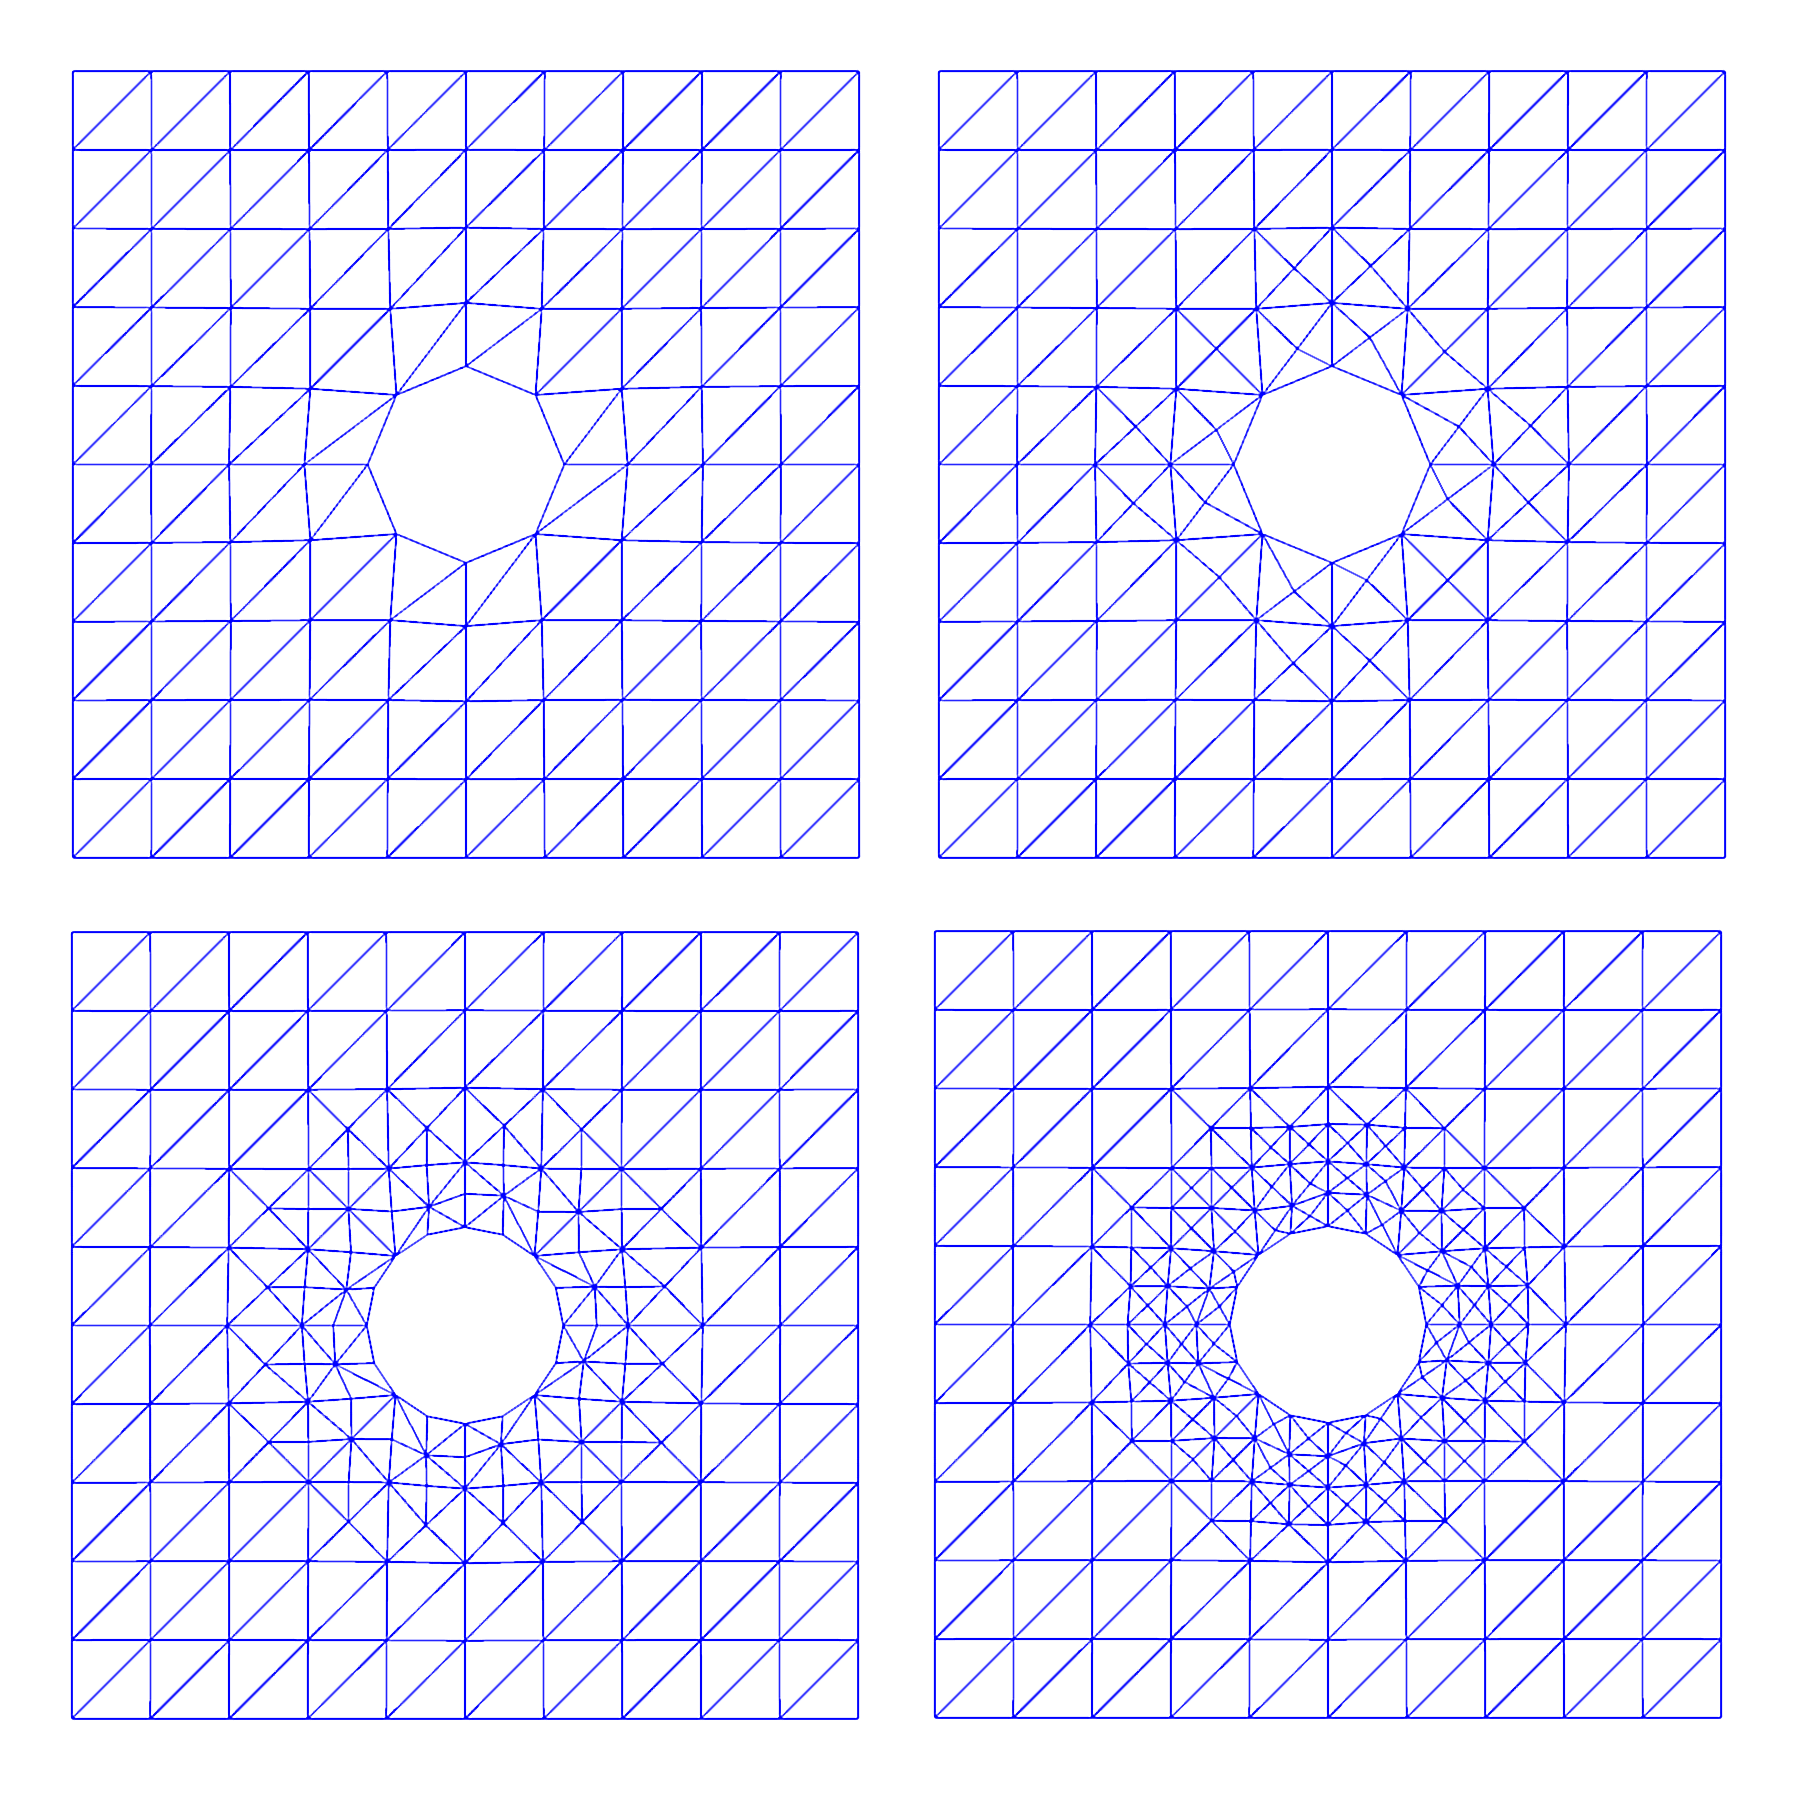
\includegraphics[width=\largefig]{chapters/kirby-7/png/refinement.png}
  \caption{A sequence of adaptively refined meshes obtained by
    successive refinement of an original coarse mesh.}
  \label{fig:refinement}
\end{figure}

%------------------------------------------------------------------------------
\section{Automating the finite element method}
\index{automation}

The FEniCS Project seeks to automate the solution of differential
equations. This is a formidable task, but it may be approached by an
automation of the finite element method. In particular, this
automation relies on the following key steps:
\begin{itemize}
\item[(i)]
  automation of discretization,
\item[(ii)]
  automation of discrete solution,
\item[(iii)]
  automation of error control.
\end{itemize}
Since its inception in~2003, the FEniCS Project has been concerned
mainly with the automation of discretization, resulting in the
development of the form compilers FFC and SyFi/SFC, the code
generation interface~UFC, the form language~UFL, and a generic
assembler implemented as part of DOLFIN. As a result, variational
problems for a large class of partial differential equations may now
be automatically discretized by the finite element method using
FEniCS. For the automation of discrete solution; that is, the solution
of linear and nonlinear systems arising from the automated
discretization of variational problems, interfaces to state-of-the-art
libraries for linear algebra have been implemented as part of
DOLFIN. Ongoing work is now seeking to automate error control by
automated error estimation and adaptivity. In the following chapters,
we return to specific aspects of the automation of the finite element
method developed as part of the FEniCS Project. The mathematical
methodology behind the FEniCS Project has also been described in
a number of scientific works. For further reading, we refer to
\citet{Logg2007a,LoggWells2010,Kirby2004,KirbyLogg2006,
AlnaesLoggMardalEtAl2009,AlnaesMardal2009b,KirbyKnepleyLoggEtAl2005,
KirbyLoggScottEtAl2006,KirbyLogg2007,KirbyLogg2008,KirbyScott2007,
Kirby2006a,OelgaardLoggWells2008,RognesKirbyLogg2009,OelgaardWells2010,
Logg2009}.

%------------------------------------------------------------------------------
\section{Historical notes}

In 1915, Boris Grigoryevich Galerkin formulated a general method for
solving differential equations~\citep{Galerkin1915}. A similar
approach was presented sometime earlier by Bubnov. Galerkin's method,
or the Bubnov--Galerkin method, was originally formulated with global
polynomials and goes back to the variational principles of Leibniz,
Euler, Lagrange, Dirichlet, Hamilton,
Castigliano \citep{Castigliano1879}, Rayleigh~\citep{Rayleigh1870} and
Ritz~\citep{Ritz1908}. Galerkin's method with piecewise polynomial
spaces $(V_h, \hat{V}_h)$ is known as the \emph{finite element
  method}. The finite element method was introduced by engineers for
structural analysis in the 1950s and was independently proposed by
Courant~\citep{Courant1943}. The exploitation of the finite element
method among engineers and mathematicians exploded in the 1960s. Since
then, the machinery of the finite element method has been expanded and
refined into a comprehensive framework for the design and analysis of
numerical methods for differential equations;
see~\citet{ZienkiewiczTaylorZhu2005firstpublishedin1967,StrangFix1973,Ciarlet1976,BeckerCareyOden1981,Hughes1987,BrennerScott2008}.
Recently, the quest for compatible (stable) discretizations of mixed
variational problems has led to the development of finite element
exterior calculus~\citep{ArnoldFalkWinther2006}.

Work on \emph{a~posteriori} error analysis of finite element methods
dates back to the pioneering work
of~\citet{BabuvskaRheinboldt1978}. Important references include the
works by~\citet{BankWeiser1985,ZienkiewiczZhu1987,
  ErikssonJohnson1991,ErikssonJohnson1995a,ErikssonJohnsonIII,ErikssonJohnson1995b,ErikssonJohnson1995c,ErikssonJohnsonLarsson1998,AinsworthOden1993}
and the reviews
papers~\citep{ErikssonEstepEtAl1995,Verfurth1994,Verfurth1999,AinsworthOden2000,BeckerRannacher2001}.

\fenicschapter{DOLFIN: A C++/Python finite element library}
              {DOLFIN: A C++/Python finite element library}
              {DOLFIN: A C++/Python finite element library}
              {Anders Logg, Garth N. Wells and Johan Hake}
              {logg-2}

DOLFIN is a C++/Python library that functions as the main user
interface of FEniCS. In this chapter, we review the functionality of
DOLFIN. We also discuss the implementation of some key features of
DOLFIN in detail. For a general discussion on the design and
implementation of DOLFIN, we refer to~\citet{LoggWells2010}.

%------------------------------------------------------------------------------
\section{Overview}
\index{DOLFIN}

A large part of the functionality of FEniCS is implemented as part of
DOLFIN. It provides a problem solving environment for models based
on partial differential equations and implements core parts of the
functionality of FEniCS, including data structures and algorithms for
computational meshes and finite element assembly. To provide a simple
and consistent user interface, DOLFIN wraps the functionality of other
FEniCS components and external software, and handles the communication
between these components.

Figure~\ref{fig:logg-2:fenicsmap} presents an overview of
the relationships between the components of FEniCS and external
software. The software map presented in the figure shows a
user application implemented on top of the DOLFIN user interface,
either in C++ or in Python. User applications may also be developed
using FEniCS Apps, a collection of solvers implemented on top of
FEniCS/DOLFIN. DOLFIN itself functions as both a user interface and a
core component of FEniCS. All communication between a user program,
other core components of FEniCS and external software is routed
through wrapper layers that are implemented as part of the DOLFIN user
interface. In particular, variational forms expressed in the UFL form
language (Chapter~\ref{chap:alnes-1}) are passed to the form compiler
FFC (Chapter~\ref{chap:logg-1}) or SFC (Chapter~\ref{chap:alnes-3})
to generate UFC code (Chapter~\ref{chap:alnes-2}), which can then
be used by DOLFIN to assemble linear systems. In the case of FFC,
this code generation depends on the finite element backend FIAT
(Chapter~\ref{chap:kirby-2}), the just-in-time compilation utility Instant
(Chapter~\ref{chap:wilbers}) and the optional optimizing backend FErari
(Chapter~\ref{chap:kirby-3}). Finally, the plotting capabilities provided
by DOLFIN are implemented by \citet{www:viper}. Some of this communication
is exposed to users of the DOLFIN C++ interface, which requires a user
to explicitly generate UFC code from a UFL form file by calling a form
compiler on the command-line.

DOLFIN also relies on external software for important functionality
such as the linear algebra libraries
\citet{www:petsc}, \citet{www:trilinos}, \citet{www:ublas} and \citet{www:mtl4}, and the
mesh partitioning libraries \citet{www:parmetis} and
SCOTCH~\citep{www:scotch}.
\begin{figure}
  \centering
  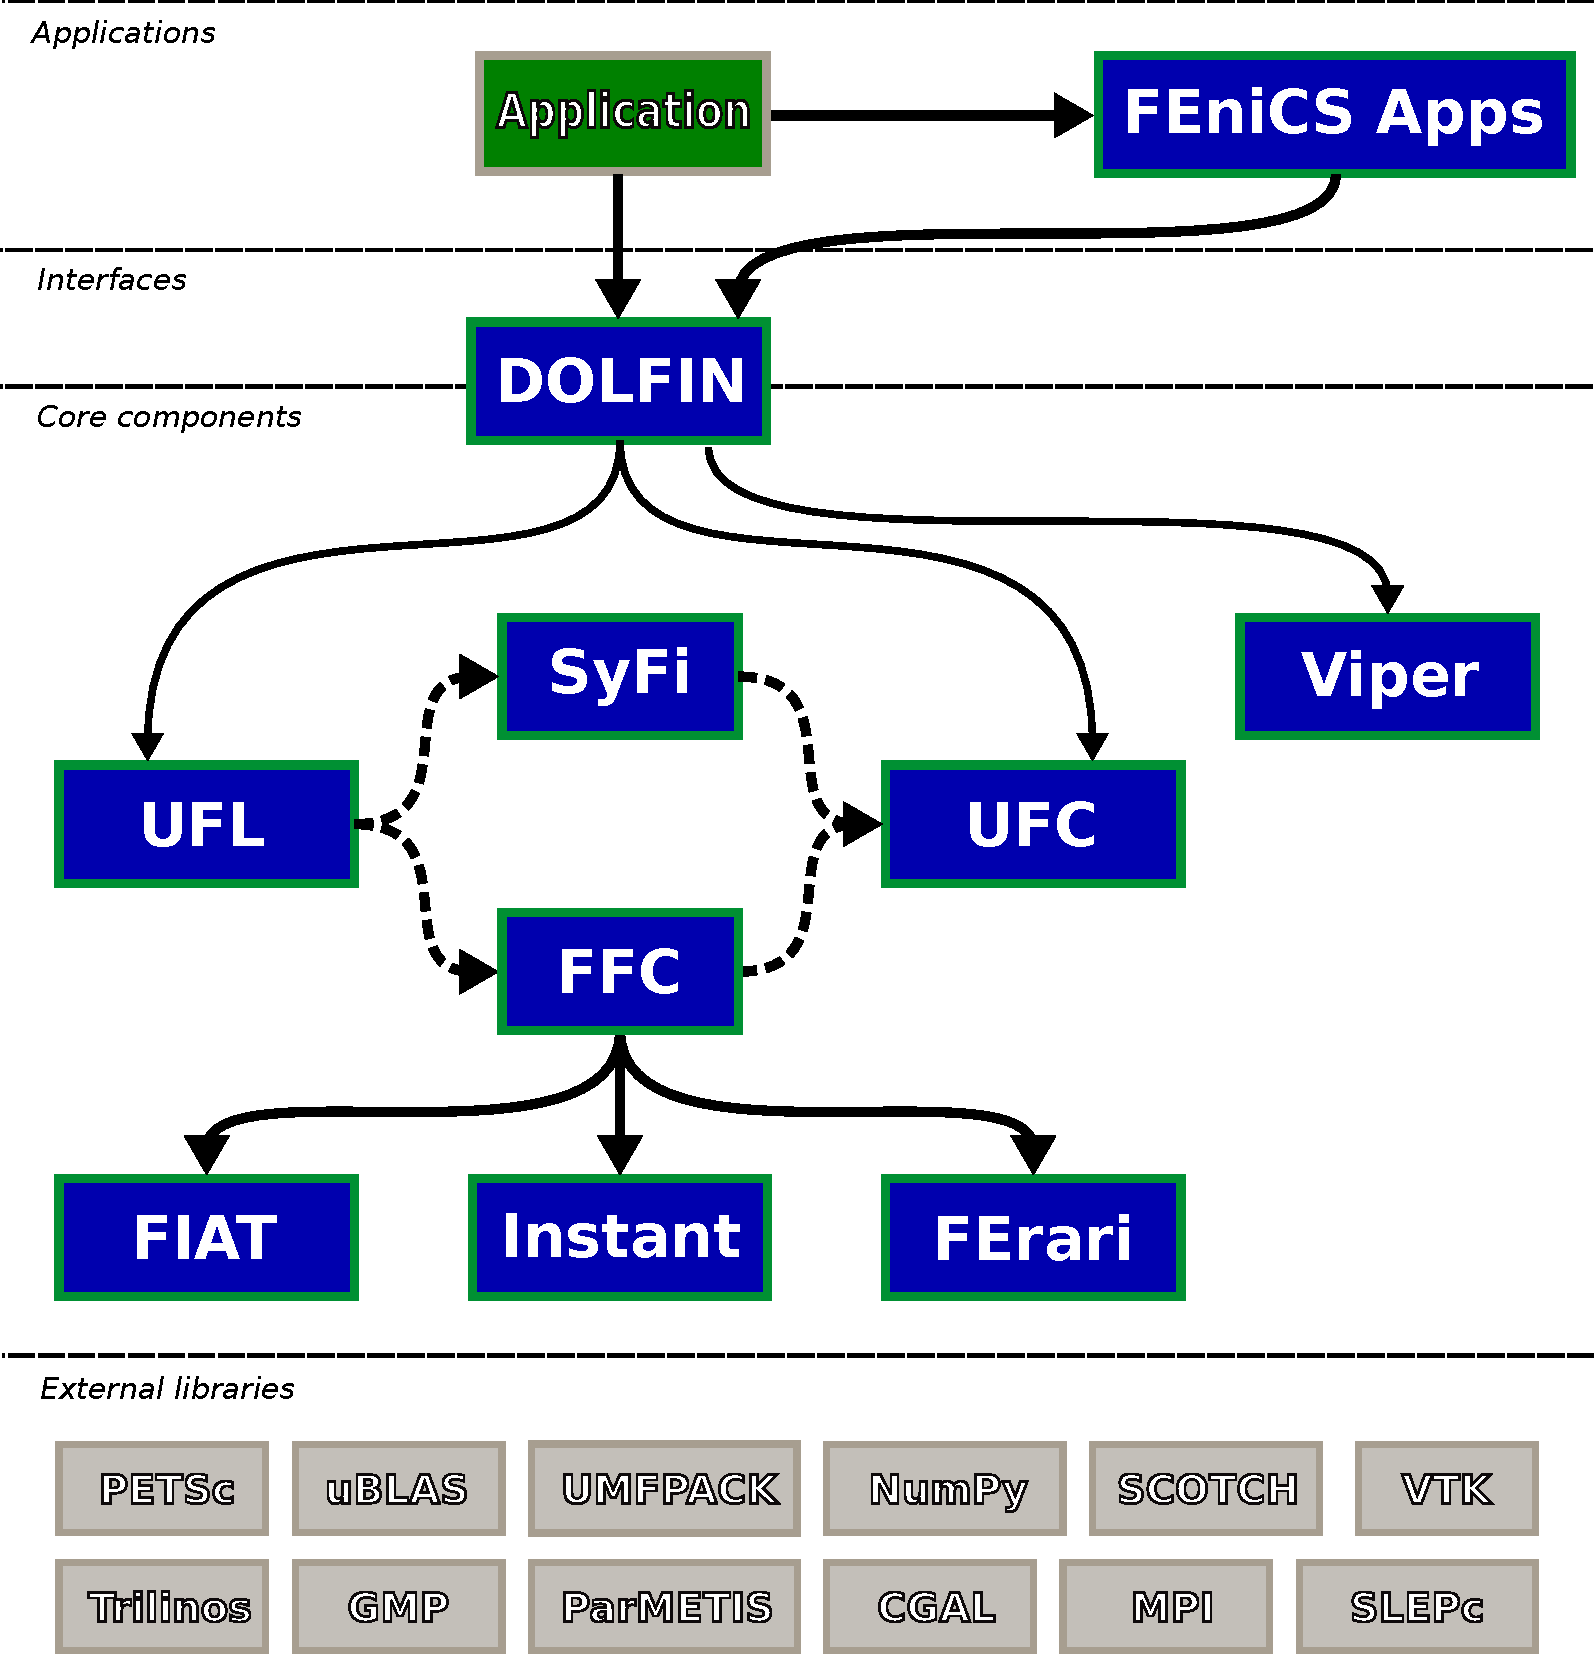
\includegraphics[width=\largefig]{chapters/logg-2/pdf/fenics-map.pdf}
  \caption{DOLFIN functions as the main user interface of FEniCS and
    handles the communication between the various components of FEniCS
    and external \hbox{software.} Solid lines indicate dependencies and
    dashed lines indicate data flow.}
  \label{fig:logg-2:fenicsmap}
\end{figure}

%------------------------------------------------------------------------------
%------------------------------------------------------------------------------
\section{User interfaces}
\index{user interfaces}

DOLFIN provides two user interfaces. One interface is implemented as a
traditional C++ library, and another interface is implemented as a
standard Python module. The two interfaces are near-identical, but in
some cases particular language features of either C++ or Python
require variations in the interfaces.  In particular, the Python
interface adds an additional level of automation by employing
run-time (just-in-time) code generation.  Below, we comment on the
design and implementation of the two user interfaces of DOLFIN.

%------------------------------------------------------------------------------
\subsection{C++ interface}
\index{user interfaces!C++}

The DOLFIN C++ interface is designed as a standard object-oriented
C++ library. It provides classes such as \emp{Matrix}, \emp{Vector},
\emp{Mesh}, \emp{FiniteElement}, \emp{FunctionSpace} and \emp{Function},
which model important concepts for finite element computing (see
Figure~\ref{fig:logg-2:uml}). It also provides a small number of free
functions (a function that is not a member function of a class),
most notably \emp{assemble} and \emp{solve}, which can be used in
conjunction with DOLFIN class objects to implement finite element
solvers. The interface is designed to be as simple as possible, and
without compromising on generality.  When external software is wrapped,
a simple and consistent user interface is provided to allow the rapid
development of solvers without needing to deal with differences in the
interfaces of external libraries. However, DOLFIN has been designed to
interact flexibly with external software. In particular, in cases where
DOLFIN provides wrappers for external libraries, such as the \emp{Matrix}
and \emp{Vector} classes which wrap data structures from linear algebra
libraries like PETSc and Trilinos, advanced users may, if necessary,
access the underlying data structures in order to use native functionality
from the wrapped external libraries.

\begin{figure}
\bwfig
  \centering
  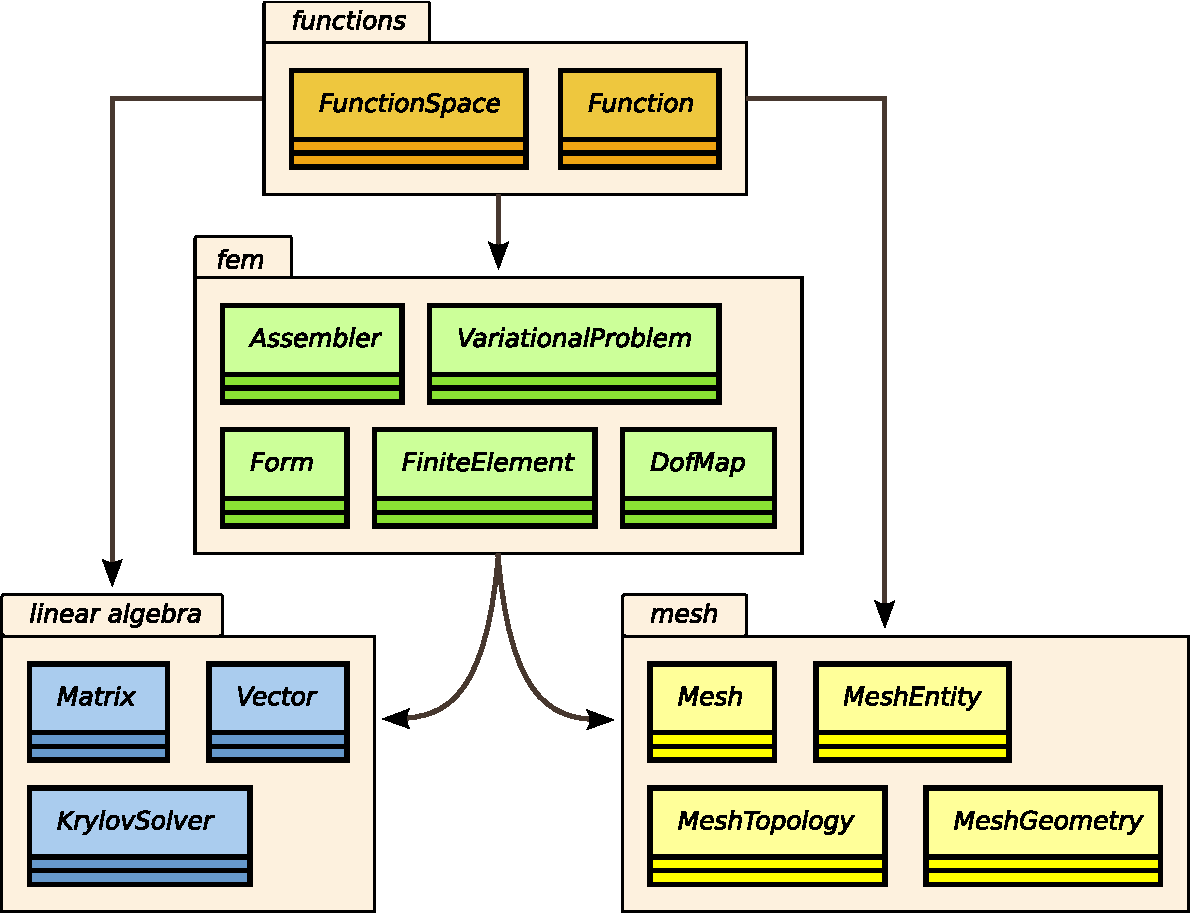
\includegraphics[width=\largefig]{chapters/logg-2/pdf/dolfin-uml.pdf}
  \caption{Schematic overview of some of the most important components
  and classes of DOLFIN. Arrows indicate dependencies.}
  \label{fig:logg-2:uml}
\end{figure}

To solve partial differential equations using the DOLFIN C++
interface, users must express finite element variational problems
in the UFL form language. This is accomplished by entering the forms
into separate \emp{.ufl} files and compiling those files using a form
compiler to generate UFC-compliant C++ code. The generated code may
then be included in a DOLFIN C++ program. We return to this issue in
Section~\ref{sec:logg-2:functionality}.

To use DOLFIN from C++, users need to include one or more header files
from the DOLFIN C++ library. In the simplest case, one includes the
header file \emp{dolfin.h}, which in turn includes all other DOLFIN
header files:

\begin{c++}
#include <dolfin.h>

using namespace dolfin;

int main()
{

  return 0;
}
\end{c++}

%------------------------------------------------------------------------------
\subsection{Python interface}
\index{user interfaces!Python}

Over the last decade, Python has emerged as an attractive choice for
the rapid development of simulation codes for scientific computing.
Python brings the benefits of a high-level scripting language, the
strength of an object-oriented language and a wealth of libraries for
numerical computation.

The bulk of the DOLFIN Python interface is automatically generated
from the C++ interface using SWIG \citep{Beazley2006,www:swig}. Since
the functionality of both the C++ and Python interfaces are
implemented as part of the DOLFIN C++ library, DOLFIN is equally
efficient via the C++ and Python interfaces for most operations.

The DOLFIN Python interface offers some functionality that is not
available from the C++ interface. In particular, the UFL form language
is seamlessly integrated into the Python interface and code generation
is automatically handled at run-time.  To use DOLFIN from Python,
users need to import functionality from the DOLFIN Python module. In
the simplest case, one includes all functionality from the Python
module named \emp{dolfin}:

\pagebreak
\begin{python}
from dolfin import *
\end{python}

%------------------------------------------------------------------------------
%------------------------------------------------------------------------------
\section{Functionality}
\label{sec:logg-2:functionality}

DOLFIN is organized as a collection of libraries (modules), with each
covering a certain area of functionality. We review here these areas
and explain the purpose and usage of the most commonly used classes and
functions. The review is bottom-up; that is, we start by describing the
core low-level functionality of DOLFIN (linear algebra and meshes) and
then move upwards to describe higher level functionality. For further
details, we refer to the DOLFIN Programmer's Reference on the FEniCS
Project web page and to \citet{LoggWells2010}.

%------------------------------------------------------------------------------
\subsection{Linear algebra}
\index{linear algebra}

DOLFIN provides a range of linear algebra objects and functionality,
including vectors, dense and sparse matrices, direct and iterative linear
solvers and eigenvalues solvers, and does so via a simple and consistent
interface.  For the bulk of underlying functionality, DOLFIN relies
on third-party libraries such as PETSc and Trilinos.  DOLFIN defines
the abstract base classes \emp{GenericTensor}, \emp{GenericMatrix}
and \emp{GenericVector}, and these are used extensively throughout the
library.  Implementations of these generic interfaces for a number of
backends are provided in DOLFIN, thereby achieving a common interface for
different backends.  Users can also wrap other linear algebra backends
by implementing the generic interfaces.

\paragraph{Matrices and vectors.}
\index{matrix}
\index{vector}
\index{\emp{Matrix}}
\index{\emp{Vector}}

The simplest way to create matrices and vectors is via the classes
\emp{Matrix} and \emp{Vector}. In general, \emp{Matrix} and \emp{Vector}
represent distributed linear algebra objects that may be stored across
(MPI) processes when running in parallel. Consistent with the most common
usage in a finite element library, a \emp{Vector} uses dense storage
and a \emp{Matrix} uses sparse storage.  A \emp{Vector} can be created
as follows:

\begin{c++}
Vector x;
\end{c++}

\begin{python}
x = Vector()
\end{python}
and a matrix can be created by:

\begin{c++}
Matrix A;
\end{c++}

\begin{python}
A = Matrix()
\end{python}
In most applications, a user may need to create a matrix or a vector,
but most operations on the linear algebra objects, including resizing,
will take place inside the library and a user will not have to operate
on the objects directly.

The following code illustrates how to create a vector of size~100:
%%
\begin{c++}
Vector x(100);
\end{c++}
%%
\begin{python}
x = Vector(100)
\end{python}
%%
A number of backends support distributed linear algebra for parallel
computation, in which case the vector \emp{x} will have global size
100, and DOLFIN will partition the vector across processes in (near)
equal-sized portions.

%To control the distribution of a vector across processes, for example,
%to match to the dimensions of locally owned degrees of freedom, a
%\emp{Vector} can be created using a local (process) range. For
%example, a vector that stores entries 20 to 79 on the local process is
%created by:
%
%\begin{c++}
%Vector x(20, 80);
%\end{c++}
%
%\begin{python}
%x = Vector(20, 80)
%\end{python}
%The vector must be created on all processes and there must be no overlap
%in the local ranges. The linear algebra backend will compute the global
%size of the vector based on the local size for each process.

Creating a \emp{Matrix} of a given size is more involved as the matrix
is sparse and in general needs to be initialized (data structures
allocated) based on the structure of the sparse matrix (its sparsity
pattern). Initialization of sparse matrices is handled by DOLFIN when
required.

While DOLFIN supports distributed linear algebra objects for parallel
computation, it is rare that a user is exposed to details at the level
of parallel data layouts. The distribution of objects across processes
is handled automatically by the library.

\paragraph{Solving linear systems.}
\index{linear system}
\index{\emp{solve}}

The simplest approach to solving the linear system $Ax = b$ is to use
%
\begin{c++}
solve(A, x, b);
\end{c++}
%
\begin{python}
solve(A, x, b)
\end{python}
%
DOLFIN will use a default method to solve the system of equations.
Optional arguments may be given to specify which algorithm to use when
solving the linear system and, in the case of an iterative method,
which preconditioner to use:
%
\begin{c++}
solve(A, x, b, "lu");
solve(A, x, b, "gmres", "ilu");
\end{c++}
%
\begin{python}
solve(A, x, b, "lu");
solve(A, x, b, "gmres", "ilu")
\end{python}
%
Which methods and preconditioners that are available depends on which
linear algebra backend DOLFIN has been configured with. To list the
available solver methods and preconditioners, the following commands
may be used:
%
\begin{c++}
list_lu_solver_methods();
list_krylov_solver_methods();
list_krylov_solver_preconditioners();
\end{c++}
%
\begin{python}
list_lu_solver_methods()
list_krylov_solver_methods()
list_krylov_solver_preconditioners()
\end{python}

\index{\emp{list\_lu\_solver\_methods}}
\index{\emp{list\_krylov\_solver\_methods}}
\index{\emp{list\_krylov\_solver\_preconditioners}}

Using the function \emp{solve} is straightforward, but it offers
little control over details of the solution process. For many
applications, it is desirable to exercise a degree of control over the
solution process and reuse solver objects throughout a simulation.

\index{\emp{LUSolver}}

The linear system $Ax = b$ can be solved using LU decomposition
(a direct method) as follows:
%
\begin{c++}
LUSolver solver(A);
solver.solve(x, b);
\end{c++}
%
\begin{python}
solver = LUSolver(A)
solver.solve(x, b)
\end{python}
%
Alternatively, the operator $A$ associated with the linear solver
can be set post-construction:
%
\begin{c++}
LUSolver solver;
solver.set_operator(A);
solver.solve(x, b);
\end{c++}
%
\begin{python}
solver = LUSolver()
solver.set_operator(A)
solver.solve(x, b)
\end{python}
%
This can be useful when passing a linear solver via a function
interface and setting the operator inside a function.

In some cases, the system $Ax = b$ may be solved a number of times for
a given matrix $A$ and different vectors $b$, or for different $A$ but with the same nonzero structure.
If the nonzero structure of $A$ does not change, then some efficiency
gains for repeated solves can be achieved by informing the LU solver
of this fact:

\begin{c++}
solver.parameters["same_nonzero_pattern"] = true;
\end{c++}

\begin{python}
solver.parameters["same_nonzero_pattern"] = True
\end{python}
In the case that $A$ does not change, the solution time for subsequent
solves can be reduced dramatically by re-using the LU factorization
of~$A$.  Re-use of the factorization is controlled by the parameter
\emp{"reuse\_factorization"}.

It is possible for some backends to prescribe the specific LU solver
to be used. This depends on the backend, which solvers that have been
configured by DOLFIN and how third-party linear algebra backends have
been configured.

The system of equations $Ax = b$ can be solved using a preconditioned
Krylov solver by:

\index{\emp{KrylovSolver}}

\begin{c++}
KrylovSolver solver(A);
solver.solve(x, b);
\end{c++}

\begin{python}
solver = KrylovSolver(A)
solver.solve(x, b)
\end{python}
The above will use a default preconditioner and solver, and default
parameters. If a \emp{KrylovSolver} is constructed without a matrix
operator $A$, the operator can be set post-construction:

\begin{c++}
KrylovSolver solver;
solver.set_operator(A);
solver.solve(x, b);
\end{c++}

\begin{python}
solver = KrylovSolver()
solver.set_operator(A)
solver.solve(x, b)
\end{python}
In some cases, it may be useful to use a preconditioner matrix $P$ that
differs from~$A$:

\begin{c++}
KrylovSolver solver;
solver.set_operators(A, P);
solver.solve(x, b);
\end{c++}

\begin{python}
solver = KrylovSolver()
solver.set_operators(A, P)
solver.solve(x, b)
\end{python}
Various parameters for Krylov solvers can be set. Some common parameters
are:

\begin{python}
solver = KrylovSolver()
solver.parameters["relative_tolerance"]      = 1.0e-6
solver.parameters["absolute_tolerance"]      = 1.0e-15
solver.parameters["divergence_limit"]        = 1.0e4
solver.parameters["maximum_iterations"]      = 10000
solver.parameters["error_on_nonconvergence"] = True
solver.parameters["nonzero_initial_guess"]   = False
\end{python}
The parameters may be set similarly from C++. Printing a summary of
the convergence of a \emp{KrylovSolver} and printing details of the
convergence history can be controlled via parameters:

\begin{c++}
KrylovSolver solver;
solver.parameters["report"] = true;
solver.parameters["monitor_convergence"] = true;
\end{c++}

\begin{python}
solver = KrylovSolver()
solver.parameters["report"] = True
solver.parameters["monitor_convergence"] = True
\end{python}
The specific Krylov solver and preconditioner to be used can be set at
construction of a solver object. The simplest approach is to set the
Krylov method and the preconditioner via string descriptions. For example:

\begin{c++}
KrylovSolver solver("gmres", "ilu");
\end{c++}

\begin{python}
solver = KrylovSolver("gmres", "ilu")
\end{python}
The above specifies the Generalized Minimum Residual (GMRES) method as
a solver, and incomplete LU (ILU) preconditioning.

\index{GMRES}
\index{ILU}

When backends such as PETSc and Trilinos are configured, a wide range
of Krylov methods and preconditioners can be applied, and a large
number of solver and preconditioner parameters can be set. In addition
to what is described here, DOLFIN provides more advanced interfaces
which permit finer control of the solution process. It is also
possible for users to provide their own preconditioners.

\paragraph{Solving eigenvalue problems.}
\index{eigenvalue problem}
\index{SLEPc}

DOLFIN uses the library SLEPc, which builds on PETSc, to solve eigenvalue
problems. The SLEPc interface works only with PETSc-based linear algebra
objects. Therefore, it is necessary to use PETSc-based objects, or to
set the default linear algebra backend to PETSc and downcast objects
(as explained in the next section). The following code illustrates
the solution of the eigenvalue problem $Ax = \lambda x$:
%%
\begin{c++}
// Create matrix
PETScMatrix A;

// Code omitted for setting the entries of A

// Create eigensolver
SLEPcEigenSolver eigensolver(A);

// Compute all eigenvalues of A
eigensolver.solve();

// Get first eigenpair
double lambda_real, lambda_complex;
PETScVector x_real, x_complex;
eigensolver.get_eigenpair(lambda_real, lambda_complex, x_real, x_complex, 0);
\end{c++}
%%
\begin{python}
# Create matrix
A = PETScMatrix()

# Code omitted for setting the entries of A

# Create eigensolver
eigensolver = SLEPcEigenSolver(A)

# Compute all eigenvalues of A
eigensolver.solve()

# Get first eigenpair
lambda_r, lambda_c, x_real, x_complex = eigensolver.get_eigenpair(0)
\end{python}
%%
The real and complex components of the eigenvalue are returned in
\emp{lambda\_real} and \emp{lambda\_complex}, respectively, and the
real and complex components of the eigenvector are
returned in \emp{x\_real} and \emp{x\_complex}, respectively.

To create a solver for the generalized eigenvalue problem $Ax = \lambda Mx$, the
eigensolver can be constructed using $A$ and~$M$:

\begin{c++}
PETScMatrix A;
PETScMatrix M;

// Code omitted for setting the entries of A and M

SLEPcEigenSolver eigensolver(A, M);
\end{c++}
\begin{python}
A = PETScMatrix()
M = PETScMatrix()

# Code omitted for setting the entries of A and M

eigensolver = SLEPcEigenSolver(A, M)
\end{python}
There are many options that a user can set via the parameter system to
control the eigenvalue problem solution process. To print a list of
available parameters, call \emp{info(eigensolver.parameters, true)}
and \emp{info(eigensolver.parameters, True)} from C++ and Python,
respectively.

\paragraph{Selecting a linear algebra backend.}

\index{linear algebra backend}
\index{PETSc}
\index{Trilinos}
\index{Epetra}
\index{uBLAS}
\index{MTL4}

The \emp{Matrix}, \emp{Vector}, \emp{LUSolver} and \emp{KrylovSolver}
objects are all based on a specific linear algebra backend.
The default backend depends on which backends are enabled when DOLFIN
is configured.  The backend can be set via the global
parameter\break \emp{"linear\_algebra\_backend"}.  To use PETSc as the linear
algebra backend:
%%
\begin{c++}
parameters["linear_algebra_backend"] = "PETSc";
\end{c++}
%%
\begin{python}
parameters["linear_algebra_backend"] = "PETSc"
\end{python}
%%
This parameter should be set before creating linear algebra
objects. To use Epetra from the Trilinos collection, the parameter
\emp{"linear\_algebra\_backend"} should be set to \emp{"Epetra"}.
For uBLAS, the parameter should be set to \emp{"uBLAS"} and for MTL4, the
parameter should be set to \emp{"MTL4"}.

Users can explicitly create linear algebra objects that use a
particular backend. Generally, such objects are prefixed with the name
of the backend. For example, a PETSc-based vector and LU solver are
created by:
%%
\begin{c++}
PETScVector x;
PETScLUSolver solver;
\end{c++}
%%
\begin{python}
x = PETScVector()
solver = PETScLUSolver()
\end{python}

\paragraph{Solving nonlinear systems.}
\index{nonlinear system}
\index{Newton's method}
\index{\emp{NewtonSolver}}

DOLFIN provides a Newton solver in the form of the class
\emp{NewtonSolver} for solving nonlinear systems of equations of the
form
%%
\begin{equation}
  F(x) = 0,
\end{equation}
%%
where $x \in \mathbb{R}^{n}$ and $F: \mathbb{R}^{n} \rightarrow
\mathbb{R}^{n}$. To solve such a problem using the DOLFIN Newton
solver, a user needs to provide a subclass of \emp{NonlinearProblem}.
The purpose of a \emp{NonlinearProblem} object is to evaluate $F$ and
the Jacobian of $F$, which will be denoted by~$J: \mathbb{R}^{n}
\rightarrow \mathbb{R}^{n} \times \mathbb{R}^{n}$. An outline of a
user-provided \emp{MyNonlinearProblem} class for solving a nonlinear
differential equation is shown below.
%%
\begin{c++}
class MyNonlinearProblem : public NonlinearProblem
{
public:

  // Constructor
  MyNonlinearProblem(const Form& L, const Form& a,
                     const BoundaryCondition& bc) : L(L), a(a), bc(bc) {}

  // User-defined residual vector F
  void F(GenericVector& b, const GenericVector& x)
  {
    assemble(b, L);
    bc.apply(b, x);
  }

  // User-defined Jacobian matrix J
  void J(GenericMatrix& A, const GenericVector& x)
  {
    assemble(A, a);
    bc.apply(A);
  }

private:

  const Form& L;
  const Form& a;
  const BoundaryCondition& bc;

};
\end{c++}
%%
A \emp{MyNonlinearProblem} object is constructed using a linear form
\emp{L}, that when assembled corresponds to $F$, and a bilinear form
\emp{a}, that when assembled corresponds to~$J$. The classes \emp{Form}
and \emp{BoundaryCondition} used in the example are discussed in more
detail later.  The same \emp{MyNon-\break linearProblem} class can be defined
in Python:
%%
\begin{python}
class MyNonlinearProblem(NonlinearProblem):
    def __init__(self, L, a, bc):
        NonlinearProblem.__init__(self)
        self.L = L
        self.a = a
        self.bc = bc
    def F(self, b, x):
        assemble(self.L, tensor=b)
        self.bc.apply(b, x)
    def J(self, A, x):
        assemble(self.a, tensor=A)
        self.bc.apply(A)
\end{python}

Once a nonlinear problem class has been defined, a \emp{NewtonSolver}
object can be created and the Newton solver can be used to compute
the solution vector $x$ to the nonlinear problem:
%%
\begin{c++}
MyNonlinearProblem problem(L, a, bc);
NewtonSolver newton_solver;

newton_solver.solve(problem, u.vector());
\end{c++}
%%
\begin{python}
problem = MyNonlinearProblem(L, a, bc)
newton_solver = NewtonSolver()

newton_solver.solve(problem, u.vector())
\end{python}
%%
A number of parameters can be set for a \emp{NewtonSolver}. Some
parameters that determine the behavior of the Newton solver are:
%%
\begin{python}
newton_solver = NewtonSolver()
newton_solver.parameters["maximum_iterations"] = 20
newton_solver.parameters["relative_tolerance"] = 1.0e-6
newton_solver.parameters["absolute_tolerance"] = 1.0e-10
newton_solver.parameters["error_on_nonconvergence"] = False
\end{python}
%%
The parameters may be set similarly from~C++.  When testing for
convergence, usually a norm of the residual $F$ is checked.  Sometimes it
is useful instead to check a norm of the iterative correction~$dx$.
This is controlled by the parameter \emp{"convergence\_criterion"}, which
can be set to \emp{"residual"}, for checking the size of the residual $F$,
or \emp{"incremental"}, for checking the size of the increment~$dx$.

For more advanced usage, a \emp{NewtonSolver} can be constructed with
arguments that specify the linear solver and preconditioner to be used
in the solution process.

%------------------------------------------------------------------------------
\subsection{Meshes}
\index{mesh}
\index{\emp{Mesh}}

A central part of DOLFIN is its mesh library and the \emp{Mesh}
class. The mesh library provides data structures and algorithms for
computational meshes, including the computation of mesh connectivity
(incidence relations), mesh refinement, mesh partitioning and mesh
intersection.

The mesh library is implemented in C++ and has been optimized to
minimize storage requirements and to enable efficient access to mesh
data. In particular, a DOLFIN mesh is stored in a small number of
contiguous arrays, on top of which a light-weight object-oriented
layer provides a~\emph{view} to the underlying data. For a detailed
discussion on the design and implementation of the mesh library, we
refer to \citet{Logg2009}.

\paragraph{Creating a mesh.}
\index{\emp{UnitSquare}}
\index{\emp{UnitCube}}

DOLFIN provides functionality for creating simple meshes, such as
meshes of unit squares and unit cubes, spheres, rectangles and
boxes. The following code demonstrates how to create a $16\times 16$
triangular mesh of the unit square (consisting of $2\times 16\times 16
= 512$ triangles) and a $16\times 16\times 16$ tetrahedral mesh of the
unit cube (consisting of $6\times 16\times 16\times 16 = 24,576$
tetrahedra).

\begin{c++}
UnitSquare unit_square(16, 16);
UnitCube unit_cube(16, 16, 16);
\end{c++}

\begin{python}
unit_square = UnitSquare(16, 16)
unit_cube = UnitCube(16, 16, 16)
\end{python}

Simplicial meshes (meshes consisting of intervals, triangles or
tetrahedra) may be constructed explicitly by specifying the cells and
vertices of the mesh. An interface for creating simplicial meshes is
provided by the class \texttt{MeshEditor}. The following code
demonstrates how to create a mesh consisting of two triangles covering
the unit square:

\index{\emp{MeshEditor}}
\index{mesh!creating}

\begin{c++}
Mesh mesh;
MeshEditor editor;
editor.open(mesh, 2, 2);
editor.init_vertices(4);
editor.init_cells(2);
editor.add_vertex(0, 0.0, 0.0);
editor.add_vertex(1, 1.0, 0.0);
editor.add_vertex(2, 1.0, 1.0);
editor.add_vertex(3, 0.0, 1.0);
editor.add_cell(0, 0, 1, 2);
editor.add_cell(1, 0, 2, 3);
editor.close();
\end{c++}

\begin{python}
mesh = Mesh();
editor = MeshEditor();
editor.open(mesh, 2, 2)
editor.init_vertices(4)
editor.init_cells(2)
editor.add_vertex(0, 0.0, 0.0)
editor.add_vertex(1, 1.0, 0.0)
editor.add_vertex(2, 1.0, 1.0)
editor.add_vertex(3, 0.0, 1.0)
editor.add_cell(0, 0, 1, 2)
editor.add_cell(1, 0, 2, 3)
editor.close()
\end{python}

\paragraph{Reading a mesh from file.}
\index{mesh!reading}

Although the built-in classes \emp{UnitSquare} and \emp{UnitCube}
are useful for testing, a typical application will need to read from
file a mesh that has been generated by an external mesh generator. To read
a mesh from file, simply supply the filename to the constructor of the
\emp{Mesh} class:
%%
\begin{c++}
Mesh mesh("mesh.xml");
\end{c++}
%%
\begin{python}
mesh = Mesh("mesh.xml")
\end{python}
%%
Meshes must be stored in the DOLFIN XML format. The following example
illustrates the XML format for a $2 \times 2$ mesh of the unit square:

\index{mesh!XML format}
\index{file formats!DOLFIN XML}

\begin{xml}
<?xml version="1.0" encoding="UTF-8"?>

<dolfin xmlns:dolfin="http://fenicsproject.org">
  <mesh celltype="triangle" dim="2">
    <vertices size="9">
      <vertex index="0" x="0" y="0"/>
      <vertex index="1" x="0.5" y="0"/>
      <vertex index="2" x="1" y="0"/>
      <vertex index="3" x="0" y="0.5"/>
      <vertex index="4" x="0.5" y="0.5"/>
      <vertex index="5" x="1" y="0.5"/>
      <vertex index="6" x="0" y="1"/>
      <vertex index="7" x="0.5" y="1"/>
      <vertex index="8" x="1" y="1"/>
    </vertices>
    <cells size="8">
      <triangle index="0" v0="0" v1="1" v2="4"/>
      <triangle index="1" v0="0" v1="3" v2="4"/>
      <triangle index="2" v0="1" v1="2" v2="5"/>
      <triangle index="3" v0="1" v1="4" v2="5"/>
      <triangle index="4" v0="3" v1="4" v2="7"/>
      <triangle index="5" v0="3" v1="6" v2="7"/>
      <triangle index="6" v0="4" v1="5" v2="8"/>
      <triangle index="7" v0="4" v1="7" v2="8"/>
    </cells>
  </mesh>
</dolfin>
\end{xml}
%%
Meshes stored in other data formats may be converted to the DOLFIN XML
format using the command \emp{dolfin-convert}, as explained in more
detail below.

\paragraph{Mesh entities.}
\index{mesh entity}

Conceptually, a \emph{mesh} (modeled by the class \emp{Mesh}), consists of
a collection of \emph{mesh entities}.  A \emph{mesh entity} is a pair $(d,
i)$, where $d$ is the topological dimension of the mesh entity and $i$
is a unique index of the mesh entity. Mesh entities are numbered within
each topological dimension from $0$ to $n_d-1$, where $n_d$ is the number
of mesh entities of topological dimension~$d$.

\begin{figure}
  \centering
  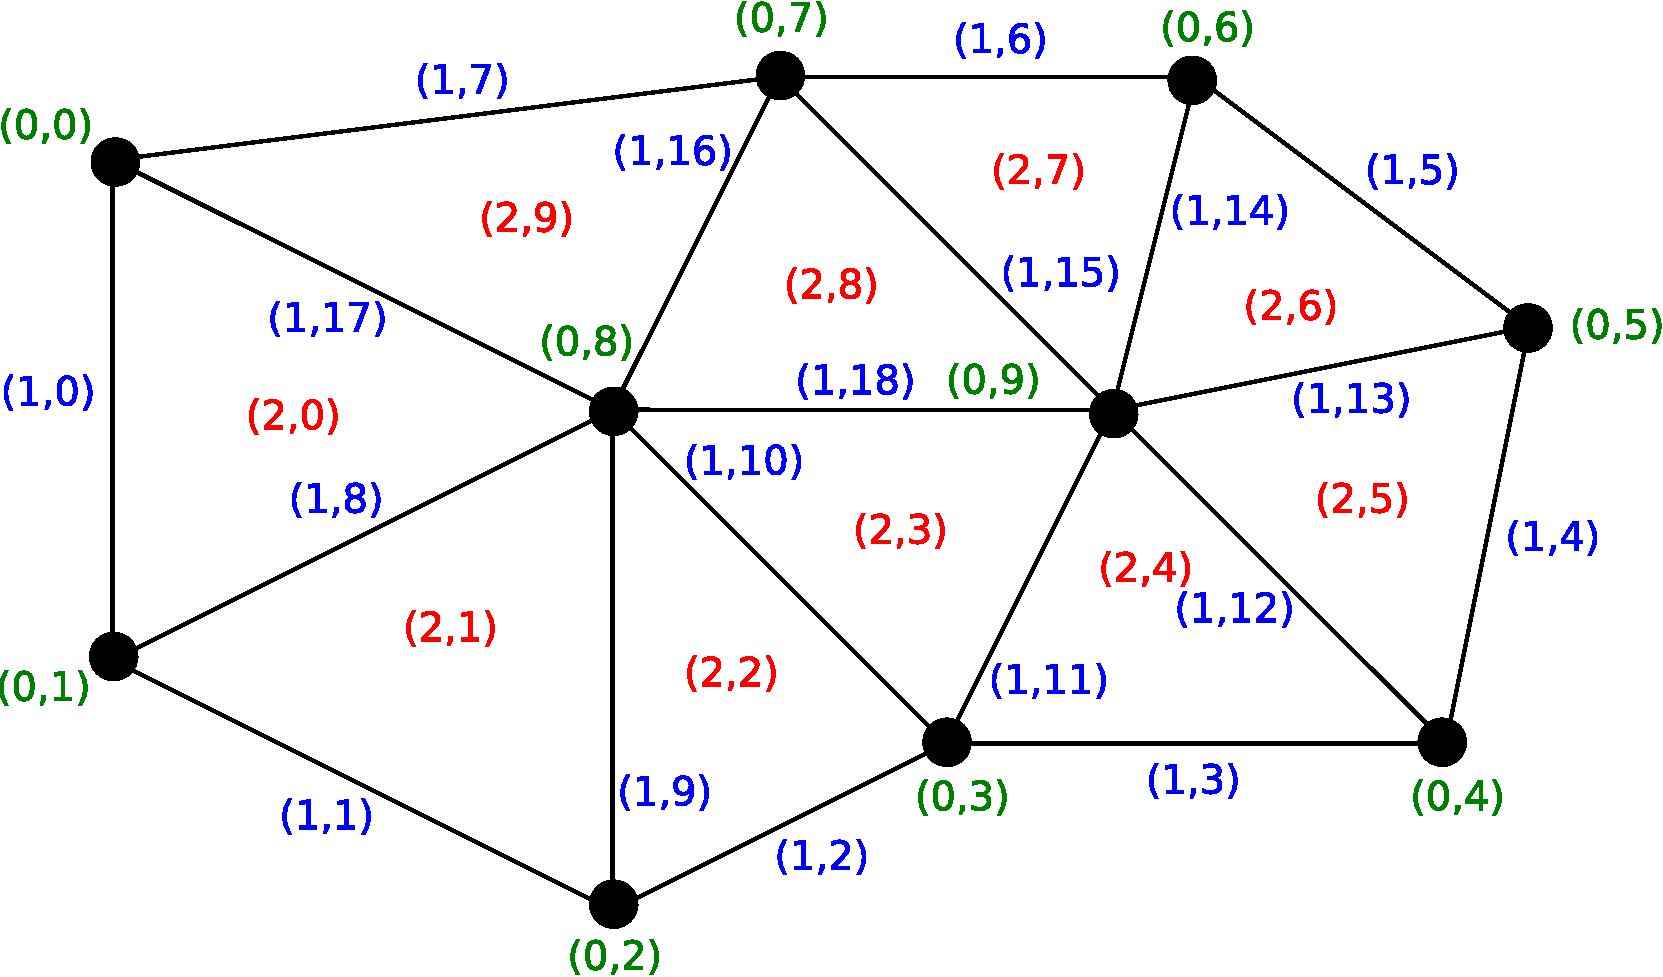
\includegraphics[width=\largefig]{chapters/logg-2/pdf/mesh-p1-entities.pdf}
  \caption{Each entity of a mesh is identified by a pair $(d, i)$
    which specifies the topological dimension~$d$ and a unique
    index~$i$ for the entity within the set of entities of
    dimension~$d$.}
  \label{fig:logg-2:entities}
\end{figure}

\index{vertex}
\index{edge}
\index{face}
\index{facet}
\index{cell}
\index{\emp{Vertex}}
\index{\emp{Edge}}
\index{\emp{Face}}
\index{\emp{Facet}}
\index{\emp{Cell}}
\index{\emp{MeshEntity}}

For convenience, mesh entities of topological dimension~$0$ are
referred to as \emph{vertices}, entities of dimension~$1$ as
\emph{edges}, entities of dimension~$2$ as \emph{faces}. Entities of
\emph{codimension}~$1$ are referred to as \emph{facets} and entities
of codimension~$0$ as \emph{cells}. These concepts are summarized in
Figure~\ref{fig:logg-2:entities} and
Table~\ref{tab:logg-2:entities}. We note that a triangular mesh
consists of vertices, edges and cells, and that the edges may
alternatively be referred to as facets and the cells as faces. We
further note that a tetrahedral mesh consists of vertices, edges,
faces and cells, and that the faces may alternatively be referred to
as facets. These concepts are implemented by the classes
\texttt{MeshEntity}, \texttt{Vertex}, \texttt{Edge}, \texttt{Face},
\texttt{Facet} and \texttt{Cell}. These classes do not store any
data. Instead, they are light-weight objects that provide views of the
underlying mesh data. A \emp{MeshEntity} may be created from a
\emp{Mesh}, a topological dimension and an index. The following code
demonstrates how to create various entities on a mesh:
%%
\begin{c++}
MeshEntity entity(mesh, 0, 33); // vertex number 33
Vertex vertex(mesh, 33);        // vertex number 33
Cell cell(mesh, 25);            // cell number 25
\end{c++}
%%
\begin{python}
entity = MeshEntity(mesh, 0, 33) # vertex number 33
vertex = Vertex(mesh, 33)        # vertex number 33
cell = Cell(mesh, 25)            # cell number 25
\end{python}

\begin{table}
  \centering
  \begin{tabular}{lcc}
    \toprule
    Entity & Dimension & Codimension \\
    \hline
    Vertex & $0$ & $D$ \\
    Edge & $1$ & $D-1$ \\
    Face & $2$ & $D-2$ \\
    & & \\
    Facet & $D-1$ & $1$ \\
    Cell & $D$ & $0$ \\
    \bottomrule
    \end{tabular}
  \caption{Mesh entities and their dimensions/codimensions. The
    codimension of an entity is $D - d$ where $D$ is the maximal
    dimension and $d$ is the dimension.}
  \label{tab:logg-2:entities}
\end{table}

\paragraph{Mesh topology and geometry.}
\index{mesh!topology}
\index{mesh!geometry}
\index{\emp{MeshTopology}}
\index{\emp{MeshGeometry}}

The topology of a mesh is stored separately from its geometry. The
topology of a mesh is a description of the relations between the
various entities of the mesh, while the geometry describes how those
entities are embedded in $\R^d$.

Users are rarely confronted with the \emp{MeshTopology} and
\emp{MeshGeometry} classes directly since most algorithms on meshes can be
expressed in terms of \emph{mesh iterators}. However, users may sometimes
need to access the dimension of a \emp{Mesh}, which involves accessing
either the \emp{MeshTopology} or \emp{MeshGeometry}, which are stored
as part of the \emp{Mesh}, as illustrated in the following code examples:
%%
\begin{c++}
uint gdim = mesh.topology().dim();
uint tdim = mesh.geometry().dim();
\end{c++}
%%
\begin{python}
gdim = mesh.topology().dim()
tdim = mesh.geometry().dim()
\end{python}
%%
It should be noted that the topological and geometric dimensions may
differ. This is the case in particular for the boundary of a mesh,
which is typically a mesh of topological dimension~$D$ embedded in
$\R^{D+1}$. That is, the geometry dimension is~$D + 1$.

\paragraph{Mesh connectivity.}
\index{mesh!connectivity}
\index{\emp{MeshConnectivity}}

The topology of a \emp{Mesh} is represented by the \emph{connectivity}
(incidence relations) of the mesh, which is a complete description of
which entities of the mesh are connected to which entities. Such
connectivity is stored in DOLFIN by the \emp{MeshConnectivity}
class. One such data set is stored as part of the class
\emp{MeshTopology} for each pair of topological dimensions $d
\rightarrow d'$ for $d, d' = 0, 1, \ldots, D$, where $D$ is the
topological dimension.

When a \emp{Mesh} is created, a minimal \emp{MeshTopology} is created.
Only the connectivity from cells (dimension~$D$) to vertices
(dimension~$0$) is stored (\emp{MeshConnectivity} $D \rightarrow 0$).
When a certain connectivity is requested, such as for example the connectivity
$1 \rightarrow 1$ (connectivity from edges to edges), DOLFIN automatically
computes any other connectivities required for computing the requested
connectivity. This is illustrated in Table~\ref{tab:logg-2:connectivity},
where we indicate which connectivities are required to compute the $1
\rightarrow 1$ connectivity.  The following code demonstrates how to
initialize various kinds of mesh connectivity for a tetrahedral mesh
($D = 3$):
%%
\begin{c++}
mesh.init(2);    // Compute faces
mesh.init(0, 0); // Compute vertex neighbors for each vertex
mesh.init(1, 1); // Compute edge neighbors for each edge
\end{c++}
%%
\begin{python}
mesh.init(2)      # Compute faces
mesh.init(0, 0)   # Compute vertex neighbors for each vertex
mesh.init(1, 1)   # Compute edge neighbors for each edge
\end{python}

\begin{table}
  \centering
  \begin{tabular}{c|cccc}
    & 0 & 1 & 2 & 3 \\
    \midrule
    0 & -- & $\times$ & -- & $\times$ \\
    1 & $\times$ & $\times$ & -- & -- \\
    2 & -- & -- & -- & -- \\
    3 & $\times$ & $\times$ & -- & $\times$ \\
  \end{tabular}
  \caption{DOLFIN computes the connectivity $d \rightarrow d'$ of a
    mesh for any pair $d, d' = 0, 1, \ldots, D$. The table
    indicates which connectivity pairs (indicated by~$\times$) have
    been computed in order to compute the connectivity $1 \rightarrow
    1$ (edge--edge connectivity) for a tetrahedral mesh.}
  \label{tab:logg-2:connectivity}
\end{table}

\paragraph{Mesh iterators.}
\index{mesh!iterators}
\index{\emp{MeshEntityIterator}}
\index{\emp{VertexIterator}}
\index{\emp{EdgeIterator}}
\index{\emp{FaceIterator}}
\index{\emp{FacetIterator}}
\index{\emp{CellIterator}}

Algorithms operating on a mesh can often be expressed in terms of
\emph{iterators}. The mesh library provides the general iterator
\texttt{MeshEntityIterator} for iteration over mesh entities,
as well as the specialized mesh iterators \texttt{VertexIterator},
\texttt{EdgeIterator}, \texttt{FaceIterator}, \texttt{FacetIterator}
and \texttt{Cell\-Iterator}.

The following code illustrates how to iterate over all incident
(connected) vertices of all vertices of all cells of a given
mesh. Two vertices are considered as neighbors if
they both belong to the same cell. For simplex meshes, this is equivalent
to an edge connecting the two vertices.
%%
\begin{c++}
for (CellIterator c(mesh); !c.end(); ++c)
  for (VertexIterator v0(*c); !v0.end(); ++v0)
    for (VertexIterator v1(*v0); !v1.end(); ++v1)
      cout << *v1 << endl;
\end{c++}
%%
\begin{python}
for c in cells(mesh):
    for v0 in vertices(c):
        for v1 in vertices(v0):
            print v1
\end{python}
%%
This may alternatively be implemented using the general iterator
\emp{MeshEntity\-Iterator} as follows:
%%
\begin{c++}
uint D = mesh.topology().dim();
for (MeshEntityIterator c(mesh, D); !c.end(); ++c)
  for (MeshEntityIterator v0(*c, 0); !v0.end(); ++v0)
    for (MeshEntityIterator v1(*v0, 0); !v1.end(); ++v1)
      cout << *v1 << endl;
\end{c++}
%%
\begin{python}
D = mesh.topology().dim()
for c in entities(mesh, D):
    for v0 in entities(c, 0):
        for v1 in entities(v0, 0):
            print v1
\end{python}

\paragraph{Mesh functions.}
\index{\emp{MeshFunction}}
\index{\emp{VertexFunction}}
\index{\emp{EdgeFunction}}
\index{\emp{FaceFunction}}
\index{\emp{FacetFunction}}
\index{\emp{CellFunction}}
\index{\emp{Point}}
\index{boundary markers}

A useful class for storing data associated with a \emp{Mesh} is the
\emp{MeshFunction} class. This makes it simple to store, for example,
material parameters, subdomain indicators, refinement markers on the
\emp{Cell}s of a \emp{Mesh} or boundary markers on the \emp{Facet}s of
a \emp{Mesh}.  A \texttt{MeshFunction} is a discrete function that takes
a value on each mesh entity of a given topological dimension~$d$. The
number of values stored in a \emp{MeshFunction} is equal to the number
of entities $n_d$ of dimension~$d$. A \texttt{MeshFunction} is templated
over the value type and may thus be used to store values of any
type. For convenience, named \texttt{MeshFunction}s are provided by the
classes \emp{VertexFunction}, \emp{EdgeFunction}, \emp{FaceFunction},
\emp{FacetFunction} and \emp{CellFunction}.  The following code
illustrates how to create a pair of \emp{MeshFunction}s, one for storing
subdomain indicators on \emp{Cell}s and one for storing boundary markers
on \emp{Facet}s:
%%
\begin{c++}
CellFunction<uint> sub_domains(mesh);
sub_domains.set_all(0);
for (CellIterator cell(mesh); !cell.end(); ++cell)
{
  Point p = cell.midpoint();
  if (p.x() > 0.5)
    sub_domains[cell] = 1;
}

FacetFunction<uint> boundary_markers(mesh);
boundary_markers.set_all(0);
for (FacetIterator facet(mesh); !facet.end(); ++facet)
{
  Point p = facet.midpoint();
  if (near(p.y(), 0.0) || near(p.y(), 1.0))
    boundary_markers[facet] = 1;
}
\end{c++}
%%
\begin{python}
sub_domains = CellFunction("uint", mesh)
sub_domains.set_all(0)
for cell in cells(mesh):
    p = cell.midpoint()
    if p.x() > 0.5:
        sub_domains[cell] = 1

boundary_markers = FacetFunction("uint", mesh)
boundary_markers.set_all(0)
for facet in facets(mesh):
    p = facet.midpoint()
    if near(p.y(), 0.0) or near(p.y(), 1.0):
        boundary_markers[facet] = 1
\end{python}


\paragraph{Mesh data.}
\index{mesh!data}
\index{\emp{MeshData}}

The \emp{MeshData} class provides a simple way to associate data with
a \emp{Mesh}. It allows arbitrary \emp{MeshFunction}s (and other
quantities) to be associated with a \emp{Mesh}. The following code
illustrates how to attach and retrieve a \emp{MeshFunction} named
\emp{"sub\_domains"} to/from a \emp{Mesh}:
%%
\begin{c++}
MeshFunction<uint>* sub_domains = mesh.data().create_mesh_function("sub_domains");
sub_domains = mesh.data().mesh_function("sub_domains");
\end{c++}
%%
\begin{python}
sub_domains = mesh.data().create_mesh_function("sub_domains")
sub_domains = mesh.data().mesh_function("sub_domains")
\end{python}
To list data associated with a given \emp{Mesh}, issue the
command \emp{info(mesh.data(), true)} in C++ or \emp{info(mesh.data(),
  True)} in Python.

\paragraph{Mesh refinement.}
\index{mesh!refinement}
\index{adaptive refinement}

A \emp{Mesh} may be refined, by either uniform or local refinement, by
calling the \emp{refine} function, as illustrated in the code examples
below.
%%
\begin{c++}
// Uniform refinement
mesh = refine(mesh);

// Local refinement
CellFunction<bool> cell_markers(mesh);
cell_markers.set_all(false);
Point origin(0.0, 0.0, 0.0);
for (CellIterator cell(mesh); !cell.end(); ++cell)
{
  Point p = cell.midpoint();
  if (p.distance(origin) < 0.1)
    cell_markers[cell] = true;
}
mesh = refine(mesh, cell_markers);
\end{c++}
%%
\begin{python}
# Uniform refinement
mesh = refine(mesh)

# Local refinement
cell_markers = CellFunction("bool", mesh)
cell_markers.set_all(False)
origin = Point(0.0, 0.0, 0.0)
for cell in cells(mesh):
    p = cell.midpoint()
    if p.distance(origin) < 0.1:
        cell_markers[cell] = True
mesh = refine(mesh, cell_markers)
\end{python}
%%
Currently, local refinement defaults to recursive refinement by edge
bisection \citep{Rivara1984,Rivara1992}. An example of a locally refined
mesh obtained by a repeated marking of the cells close to one of the
corners of the unit cube is shown in Figure~\ref{fig:logg-2:refinement}.

\begin{figure}
  \centering
  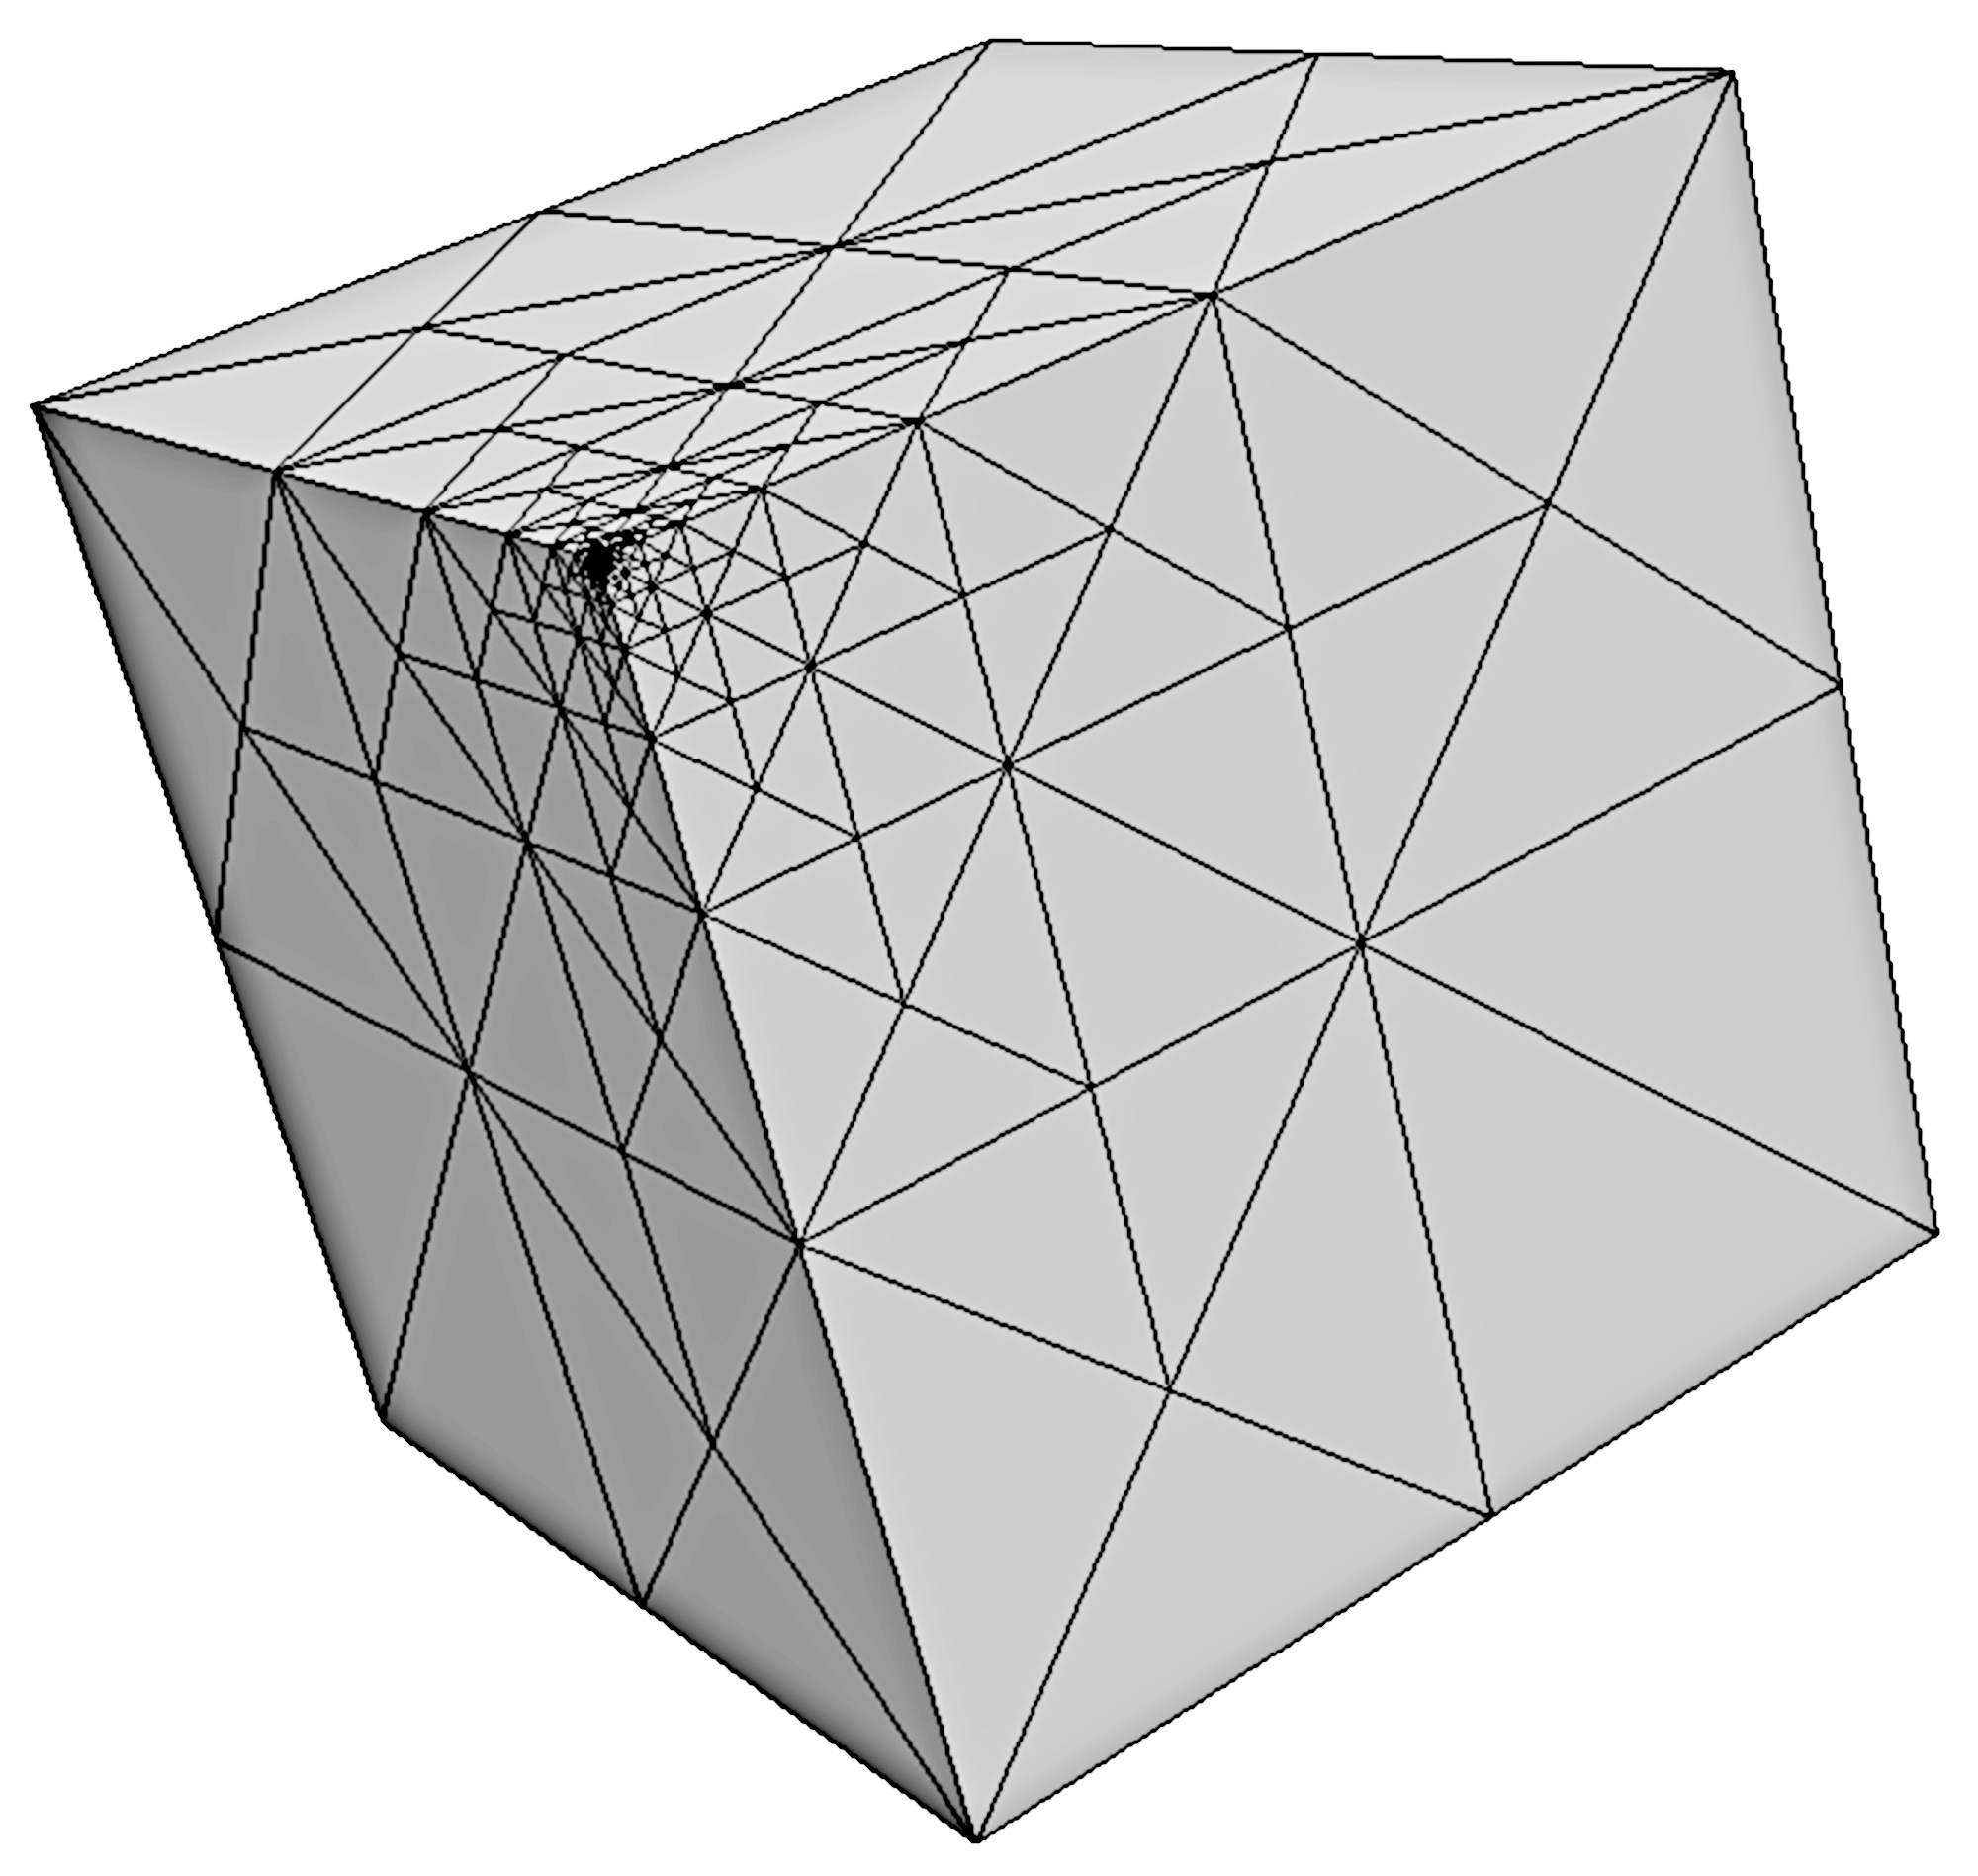
\includegraphics[width=\smallfig]{chapters/logg-2/png/refined_cube.png}
  \caption{A locally refined mesh obtained by repeated marking of the
    cells close to one of the corners of the unit cube.}
  \label{fig:logg-2:refinement}
\end{figure}

\paragraph{Parallel meshes.}
\index{mesh!distributed}

When running a program in parallel on a distributed memory architecture
(using MPI by invoking the program with the \emp{mpirun} wrapper),
DOLFIN automatically partitions and distributes meshes. Each process
then stores a portion of the global mesh as a standard \emp{Mesh}
object. In addition, it stores auxiliary data needed for correctly
computing local-to-global maps on each process and for communicating
data to neighboring regions. Parallel computing with DOLFIN is discussed
in Section~\ref{sec:logg-2:implementation}.

%------------------------------------------------------------------------------
\subsection{Finite elements}
\index{finite element!implementation}
\index{\emp{FiniteElement}}

The concept of a finite element as discussed in
Chapters~\ref{chap:kirby-7} and~\ref{chap:kirby-6} (the Ciarlet
definition) is implemented by the DOLFIN \emp{FiniteElement} class. This
class is implemented differently in the C++ and Python interfaces.

The C++ implementation of the \emp{FiniteElement} class relies on
code generated by a form compiler such as FFC or SFC, which are discussed
in Chapters~\ref{chap:logg-1} and~\ref{chap:alnes-3}, respectively. The
class \emp{FiniteElement} is essentially a wrapper class for the UFC class
\emp{ufc::finite\_element}. A C++ \emp{FiniteElement} provides all
the functionality of a \emp{ufc::finite\_element}. Users of the DOLFIN C++
interface will typically not use the \emp{FiniteElement} class directly,
but it is an important building block for the \emp{FunctionSpace} class, which
is discussed below. However, users developing advanced algorithms that
require run-time evaluation of finite element basis function will need
to familiarize themselves with the \emp{FiniteElement} interface. For
details, we refer to the DOLFIN Programmer's Reference.

The Python interface also provides a \emp{FiniteElement} class.
The Python \emp{FiniteElement} class is
imported directly from the UFL Python module (see
Chapter~\ref{chap:alnes-1}). As such, it is just a label for a
particular finite element that can be used to define variational
problems. Variational problems are more conveniently defined in
terms of the DOLFIN \emp{FunctionSpace} class,
so users of the Python interface are rarely confronted with
the \emp{FiniteElement} class. However, advanced users who wish to
develop algorithms in Python that require functionality defined in the
UFC interface, such as run-time evaluation of basis functions, can
access such functionality by explicitly generating code from within
the Python interface. This can be accomplished by a call to the
DOLFIN \emp{jit} function (just-in-time compilation), which takes as
input a UFL \emp{FiniteElement} and returns a pair containing a
\emp{ufc::finite\_element} and a \emp{ufc::dofmap}. The returned
objects are created by first generating the corresponding C++ code,
then compiling and wrapping that C++ code into a Python module. The
returned objects are therefore directly usable from within Python.

The degrees of freedom of a \emp{FiniteElement} can be plotted directly
from the Python interface by a call to \emp{plot(element)}. This will
draw a picture of the shape of the finite element, along with a graphical
representation of its degrees of freedom in accordance with the notation
described in Chapter~\ref{chap:kirby-6}.

Table~\ref{tab:logg-2:elements} lists the finite elements currently
supported by DOLFIN (and the toolchain FIAT--UFL--FFC/SFC--UFC). A
\emp{FiniteElement} may be specified (from Python) using either its full
name or its short symbol, as illustrated in the code example below:
%%
\begin{uflcode}
element = FiniteElement("Lagrange", tetrahedron, 5)
element = FiniteElement("CG", tetrahedron, 5)

element = FiniteElement("Brezzi-Douglas-Marini", triangle, 3)
element = FiniteElement("BDM", triangle, 3)

element = FiniteElement("Nedelec 1st kind H(curl)", tetrahedron, 2)
element = FiniteElement("N1curl", tetrahedron, 2)
\end{uflcode}

\begin{table}
  \index{finite element!list of supported}
  \centering
  \begin{tabular}{ll}
    \toprule
    Name & Symbol \\
    \midrule
    \grey{\it Argyris} & \grey{\it ARG} \\
    \grey{\it Arnold--Winther} & \grey{\it AW} \\
    Brezzi--Douglas--Marini & BDM \\
    Crouzeix--Raviart & CR \\
    Discontinuous Lagrange & DG \\
    \grey{\it Hermite} & \grey{\it HER} \\
    Lagrange & CG \\
    \grey{\it Mardal--Tai--Winther} & \grey{\it MTW} \\
    \grey{\it Morley} & \grey{\it MOR} \\
    \nedelec{} 1st kind $\Hcurl$ & N1curl \\
    \nedelec{} 2nd kind $\Hcurl$ & N2curl \\
    Raviart--Thomas & RT \\
    \bottomrule
    \end{tabular}
  \caption{List of finite elements supported by DOLFIN~1.0. Elements
    in grey italics are partly supported in FEniCS but not
    throughout the entire toolchain.}
  \label{tab:logg-2:elements}
\end{table}

%------------------------------------------------------------------------------
\subsection{Function spaces}
\index{function space}
\index{\emp{FunctionSpace}}
\index{\emp{DofMap}}

The DOLFIN \emp{FunctionSpace} class represents a finite element function
space~$V_h$, as defined in Chapter~\ref{chap:kirby-7}. The data of a
\emp{FunctionSpace} is represented in terms of a triplet consisting of
a \emp{Mesh}, a \emp{DofMap} and a \emp{FiniteElement}:
%%
\begin{verse}
  \centering
  \emp{FunctionSpace} = (\emp{Mesh},\; \emp{DofMap},\; \emp{FiniteElement}).
\end{verse}
%%
The \emp{Mesh} defines the computational domain and its
discretization. The \emp{DofMap} defines how the degrees of freedom
of the function space are distributed. In particular, the \emp{DofMap}
provides the function \emp{tabulate\_dofs} which maps the local degrees
of freedom on any given cell of the \emp{Mesh} to global degrees of
freedom. The \emp{DofMap} plays a role in defining the global regularity
of the finite element function space.  The \emp{FiniteElement} defines
the local function space on any given cell of the \emp{Mesh}. Note that
if two or more \emp{FunctionSpace}s are created on the same \emp{Mesh},
that \emp{Mesh} is shared between the two \emp{FunctionSpace}s.

\paragraph{Creating function spaces.}

As for the \emp{FiniteElement} class, \emp{FunctionSpace}s are handled
differently in the C++ and Python interfaces. In C++, the instantiation
of a \emp{FunctionSpace} relies on generated code. As an example,
we consider here the creation of a \emp{FunctionSpace} representing
continuous piecewise linear Lagrange polynomials on triangles. First,
the corresponding finite element must be defined in the UFL form
language. We do this by entering the following code into a file named
\emp{Lagrange.ufl}:
%%
\begin{uflcode}
element = FiniteElement("Lagrange", triangle, 1)
\end{uflcode}
%%
We may then generate C++ code using a form compiler such as FFC:
%%
\begin{bash}
ffc -l dolfin Lagrange.ufl
\end{bash}
This generates a file named \emp{Lagrange.h} that we may include in
our C++ program to instantiate a \emp{FunctionSpace} on a given
\emp{Mesh}:
%%
\begin{c++}
#include <dolfin.h>
#include "Lagrange.h"

using namespace dolfin;

int main()
{
  UnitSquare mesh(8, 8);
  Lagrange::FunctionSpace V(mesh);

  ...
  return 0;
}
\end{c++}
%%
In typical applications, a \emp{FunctionSpace} is not generated
through a separate \emp{.ufl} file, but is instead generated as part
of the code generation for a variational problem.

From the Python interface, one may create a \emp{FunctionSpace}
directly, as illustrated by the following code which creates the same
function space as the above example (piecewise linear Lagrange
polynomials on triangles):

\begin{python}
mesh = UnitSquare(8, 8)
V = FunctionSpace(mesh, "Lagrange", 1)
\end{python}

\paragraph{Mixed spaces.}
\index{function space!mixed}
\index{mixed function space}

Mixed function spaces may be created from arbitrary combinations of
function spaces. As an example, we consider here the creation of the
\emph{Taylor--Hood} function space for the discretization of the
Stokes or incompressible Navier--Stokes equations. This mixed function
space is the tensor product of a vector-valued continuous piecewise
quadratic function space for the velocity field and a scalar
continuous piecewise linear function space for the pressure
field. This may be easily defined in either a UFL form file (for code
generation and subsequent inclusion in a C++ program) or directly in a
Python script as illustrated in the following code examples:
%%
\begin{uflcode}
V = VectorElement("Lagrange", triangle, 2)
Q = FiniteElement("Lagrange", triangle, 1)
W = V*Q
\end{uflcode}
%
\begin{python}
V = VectorFunctionSpace(mesh, "Lagrange", 2)
Q = FunctionSpace(mesh, "Lagrange", 1)
W = V*Q
\end{python}

DOLFIN allows the generation of arbitrarily nested mixed function
spaces. A mixed function space can be used as a building block in the
construction of a larger mixed space. When a mixed function space is
created from more than two function spaces (nested on the same level),
then one must use the \emp{MixedElement} constructor (in UFL/C++) or
the \emp{MixedFunctionSpace} constructor (in Python). This is because
Python will interpret the expression \emp{V*Q*P} as \emp{(V*Q)*P},
which will create a mixed function space consisting of two subspaces:
the mixed space \emp{V*Q} and the space \emp{P}. If that is not the
intention, one must instead define the mixed function space using
\emp{MixedElement([V, Q, P])} in UFL/C++ or
\emp{MixedFunctionSpace([V, Q, P])} in Python.

\paragraph{Subspaces.}
\index{function space!subspace}

For a mixed function space, one may access its subspaces. These
subspaces differ, in general, from the function spaces that were used to
create the mixed space in their degree of freedom maps (\emp{DofMap}
objects). Subspaces are particularly useful for applying boundary
conditions to components of a mixed element. We return to this
issue below.

%------------------------------------------------------------------------------
\subsection{Functions}
\index{function}
\index{\emp{Function}}

The \emp{Function} class represents a finite element
function~$u_h$ in a finite element space~$V_h$ as defined in
Chapter~\ref{chap:kirby-7}:
%%
\begin{equation}
  u_h(x) = \sum_{j=1}^N U_j \phi_j(x),
\end{equation}
%%
where $U \in \R^N$ is the vector of degrees of freedom for the
function~$u_h$ and $\{\phi_j\}_{j=1}^N$ is a basis for $V_h$.  A
\emp{Function} is represented in terms of a \emp{FunctionSpace} and a
\emp{GenericVector}:
%%
\begin{verse}
  \centering
  \emp{Function} = (\emp{FunctionSpace},\; \emp{GenericVector}).
\end{verse}
%%
The \emp{FunctionSpace} defines the function space $V_h$ and the
\emp{GenericVector} holds the vector~$U$ of degrees of freedom; see
Figure~\ref{fig:logg-2:femsolution}. When running in parallel on a
distributed memory architecture, the \emp{FunctionSpace} and the
\emp{GenericVector} are distributed across the processes.

\begin{figure}
\bwfig
  \centering
  \fenicsfig{logg-2}{femsolution}{\mediumfig}
  \caption{A piecewise linear finite element function~$u_h$ on a
    mesh consisting of triangular elements. The vector of degrees of
    freedom~$U$ is given by the values of~$u_h$ at the mesh
    vertices.}
  \label{fig:logg-2:femsolution}
\end{figure}

\enlargethispage{12pt}

\paragraph{Creating functions.}
\emp{function!creation}

\looseness-1{}To create a \emp{Function} on a \emp{FunctionSpace}, one simply calls
the constructor of the \emp{Function} class with the \emp{FunctionSpace}
as the argument, as illustrated in the following code examples:
%%
\begin{c++}
Function u(V);
\end{c++}
%%
\begin{python}
u = Function(V)
\end{python}
%%
If two or more \emp{Function}s are created on the same
\emp{FunctionSpace}, the \emp{FunctionSpace} is shared between the
\emp{Function}s.

A \emp{Function} is typically used to hold the computed solution to a
partial differential equation. One may then obtain the degrees of
freedom $U$ by solving a system of equations, as illustrated in the
following code examples:
%%
\begin{c++}
Function u(V);
solve(A, u.vector(), b);
\end{c++}
%%
\begin{python}
u = Function(V)
solve(A, u.vector(), b)
\end{python}
%%
The process of assembling and solving a linear system is handled
automatically by the
classes\break \emp{Linear/NonlinearVariational\-Solver}, which will be
discussed in more detail below.

\paragraph{Function evaluation.}
\index{function!evaluation}

A \emp{Function} may be evaluated at arbitrary points inside the
computational domain\footnote{One may also evaluate a \emp{Function}
  outside of the computational domain by setting the global parameter value
  \emp{"allow\_extrapolation"} to true. This may sometimes be
  necessary when evaluating a \emp{Function} on the boundary of a
  domain since round-off errors may result in points slightly outside
  of the domain.}. The value of a \emp{Function} is computed by first
locating the cell of the mesh containing the given point, and then
evaluating the linear combination of basis functions on that cell. Finding
the cell exploits an efficient search tree
algorithm that is implemented as part of \citet{www:cgal}.

The following code examples illustrate function evaluation in the C++
and Python interfaces for scalar- and vector-valued functions:
%%
\begin{c++}
# Evaluation of scalar function
double scalar = u(0.1, 0.2, 0.3);

# Evaluation of vector-valued function
Array<double> vector(3);
u(vector, 0.1, 0.2, 0.3);
\end{c++}
%%
\begin{python}
# Evaluation of scalar function
scalar = u(0.1, 0.2, 0.3)

# Evaluation of vector-valued function
vector = u(0.1, 0.2, 0.3)
\end{python}
%%
When running in parallel with a distributed mesh, functions can only be
evaluated at points located in the portion of the mesh that is stored
by the local process.

\paragraph{Subfunctions.}
\index{function!subfunction}

For \emp{Function}s constructed on a mixed \emp{FunctionSpace},
subfunctions (components) of the \emp{Function} can be accessed, for
example to plot the solution components of a mixed system. Subfunctions
may be accessed as either \emph{shallow} or \emph{deep copies}. By
default, subfunctions are accessed as shallow copies, which means that
the subfunctions share data with their parent functions.  They provide
\emph{views} to the data of the parent function. Sometimes, it may also be
desirable to access subfunctions as deep copies. A deep copied subfunction
does not share its data (namely, the vector holding the degrees of
freedom) with the parent \emp{Function}.  Both shallow and deep copies
of \emp{Function} objects are themselves \emp{Function} objects and may
(with some exceptions) be used as regular \emp{Function} objects.

Creating shallow and deep copies of subfunctions is done
differently in C++ and Python, as illustrated by the following code
examples:
%%
\begin{c++}
Function w(W);

// Create shallow copies
Function& u = w[0];
Function& p = w[1];

// Create deep copies
Function uu = w[0];
Function pp = w[1];
\end{c++}
%%
\begin{python}
w = Function(W)

# Create shallow copies
u, p = w.split()

# Create deep copies
uu, pp = w.split(deepcopy=True)
\end{python}
%%
Note that component access, such as \emp{w[0]}, from the Python
interface does not create a new \emp{Function} object as in the C++
interface. Instead, it creates a UFL expression that denotes a
component of the original \emp{Function}.

%------------------------------------------------------------------------------
\subsection{Expressions}
\index{expression}
\index{\emp{Expression}}

The \emp{Expression} class is closely related to the \emp{Function}
class in that it represents a function that can be evaluated on a
finite element space. However, where a \emp{Function} must be defined
in terms of a vector of degrees of freedom, an \emp{Expression} may be
freely defined in terms of, for example, coordinate values, other
geometric entities, or a table lookup.

An \emp{Expression} may be defined in both C++ and Python by
subclassing the \emp{Expression} class and overloading the \emp{eval}
function, as illustrated in the following code examples which define
the function $f(x, y) = \sin x \, \cos y$ as an \emp{Expression}:
%%
\begin{c++}
class MyExpression : public Expression
{
  void eval(Array<double>& values, const Array<double>& x) const
  {
    values[0] = sin(x[0])*cos(x[1]);
  }
};

MyExpression f;
\end{c++}
%%
\begin{python}
class MyExpression(Expression):
    def eval(self, values, x):
        values[0] = sin(x[0])*cos(x[1])

f = MyExpression()
\end{python}
%%
For vector-valued (or tensor-valued) \emp{Expression}s, one must also
specify the value shape of the \emp{Expression}. The following code
examples demonstrate how to implement the vector-valued function $g(x,
y) = (\sin x, \cos y)$. The value shape is defined slightly
differently in C++ and Python.
%%
\begin{c++}
class MyExpression : public Expression
{
  void eval(Array<double>& values, const Array<double>& x) const
  {
    values[0] = sin(x[0]);
    values[1] = cos(x[1]);
  }

  uint value_rank() const
  {
    return 1;
  }

  uint value_dimension(uint i) const
  {
    return 2;
  }
};

MyExpression g;
\end{c++}
%%
\begin{python}
class MyExpression(Expression):

    def eval(self, values, x):
        values[0] = sin(x[0])
        values[1] = cos(x[1])

    def value_shape(self):
        return (2,)

g = MyExpression()
\end{python}

The above \emph{functor} construct for the definition of expressions
is powerful and allows a user to define complex expressions, the
evaluation of which may involve arbitrary operations as part of the
\emp{eval} function. For simple expressions like $f(x, y) = \sin x \,
\cos y$ and $g(x, y) = (\sin x, \cos y)$, users of the Python
interface may, alternatively, use a simpler syntax:
%%
\begin{python}
f = Expression("sin(x[0])*cos(x[1])")
g = Expression(("sin(x[0])", "cos(x[1])"))
\end{python}
%%
The above code will automatically generate subclasses of the DOLFIN C++
\emp{Expression} class that overload the \emp{eval} function. This has the
advantage of being more efficient, since the callback to the \emp{eval}
function takes place in C++ rather than in Python.

\enlargethispage{12pt}

A feature that can be used to implement a time-dependent \emp{Expression}
in the Python interface is to use a variable name in an \emp{Expression}
string.  For example, one may use the variable \emp{t} to denote time:
%%
\begin{python}
h = Expression("t*sin(x[0])*cos(x[1])", t=0.0)
while t < T:
    h.t = t
    ...
    t += dt
\end{python}
%%
The \emp{t} variable has here been used to create a time-dependent
\emp{Expression}. Arbitrary variable names may be used as long as they
do not conflict with the names of built-in functions, such as \emp{sin}
or~\emp{exp}.

In addition to the above examples, the Python interface allows
the direct definition of (more complex) subclasses of the C++
\emp{Expression} class by supplying C++ code for their definition. For
more information, we refer to the DOLFIN Programmer's Reference.

%------------------------------------------------------------------------------
\subsection{Variational forms}
\index{variational form}

DOLFIN relies on the FEniCS toolchain FIAT--UFL--FFC/SFC--UFC for the
evaluation of finite element variational forms. Variational forms
expressed in the UFL form language (Chapter~\ref{chap:alnes-1})
are compiled using one of the form compilers FFC or SFC
(Chapters~\ref{chap:logg-1} and~\ref{chap:alnes-3}), and the generated
UFC code (Chapter~\ref{chap:alnes-2}) is used by DOLFIN to
evaluate (assemble) variational forms.

The UFL form language allows a wide range of variational forms to be
expressed in a language close to the mathematical notation, as exemplified
by the following expressions defining (in part) the bilinear and linear
forms for the discretization of a linear elastic problem:
%%
\begin{uflcode}
a = inner(sigma(u), epsilon(v))*dx
L = dot(f, v)*dx
\end{uflcode}
%%
This should be compared to the corresponding mathematical notation:
%%
\begin{align} \label{eq:logg-2:elasticity1}
  a(u, v) &= \int_{\Omega} \sigma(u) : \epsilon(v) \dx,
\\
  L(v)    &= \int_{\Omega} f \cdot v \dx.
\end{align}
%%
Here, $\epsilon(v) = (\Grad v + (\Grad v)^{T}) / 2$ denotes the
symmetric gradient and $\sigma(v) = 2 \mu \, \epsilon(v) + \lambda
\mathrm{tr} \, \epsilon(v) I$ is the stress tensor. For a detailed
presentation of the UFL form language, we refer to
Chapter~\ref{chap:alnes-1}.

The code generation process must be handled explicitly by users of the C++
interface by calling a form compiler on the command-line. To solve the
linear elastic problem above for a specific choice of parameter values
(the Lam\'e constants~$\mu$ and~$\lambda$), a user may enter the following
code in a file named \emp{Elasticity.ufl}\footnote{Note that `lambda'
has been deliberately misspelled since it is a reserved keyword
in Python.}:
%%
\begin{uflcode}
V = VectorElement("Lagrange", tetrahedron, 1)

u = TrialFunction(V)
v = TestFunction(V)
f = Coefficient(V)

E  = 10.0
nu = 0.3

mu    = E / (2.0*(1.0 + nu))
lmbda = E*nu / ((1.0 + nu)*(1.0 - 2.0*nu))

def sigma(v):
    return 2.0*mu*sym(grad(v)) + lmbda*tr(sym(grad(v)))*Identity(v.cell().d)

a = inner(sigma(u), sym(grad(v)))*dx
L = dot(f, v)*dx
\end{uflcode}
%%
This code may be compiled using a UFL/UFC compliant form compiler to
generate UFC C++ code. For example, using FFC:
%%
\begin{bash}
ffc -l dolfin Elasticity.ufl
\end{bash}
%%
This generates a C++ header file (including implementation) named
\emp{Elasticity.h} which may be included in a C++ program and used to
instantiate the two forms~\emp{a} and~\emp{L}:
%%
\begin{c++}
#include <dolfin.h>
#include "Elasticity.h"

using namespace dolfin;

int main()
{
  UnitSquare mesh(8, 8);
  Elasticity::FunctionSpace V(mesh);
  Elasticity::BilinearForm a(V, V);
  Elasticity::LinearForm L(V);
  MyExpression f; // code for the definition of MyExpression omitted
  L.f = f;

  return 0;
}
\end{c++}
%%
The instantiation of the forms involves the instantiation of the
\emp{FunctionSpace} on which the forms are defined. Any coefficients
appearing in the definition of the forms (here the right-hand side
\emp{f}) must be attached after the creation of the forms.

Python users may rely on automated code generation, and define variational
forms directly as part of a Python script:
%%
\begin{python}
from dolfin import *

mesh = UnitSquare(8, 8)
V = VectorElement(mesh, "Lagrange", 1)

u = TrialFunction(V)
v = TestFunction(V)
f = MyExpression() # code emitted for the definition of f

E  = 10.0
nu = 0.3

mu    = E / (2.0*(1.0 + nu))
lmbda = E*nu / ((1.0 + nu)*(1.0 - 2.0*nu))

def sigma(v):
    return 2.0*mu*sym(grad(v)) + lmbda*tr(sym(grad(v)))*Identity(v.cell().d)

a = inner(sigma(u), sym(grad(v)))*dx
L = dot(f, v)*dx
\end{python}
%%
This script will trigger automatic code generation for the definition
of the \emp{FunctionSpace}~\emp{V}. Code generation of the two
forms~\emp{a} and~\emp{L} is postponed until the point when the
corresponding discrete operators (the matrix and vector) are
assembled.

%------------------------------------------------------------------------------
\subsection{Finite element assembly}
\index{assembly!implementation}
\index{\emp{assemble}}

A core functionality of DOLFIN is the assembly of finite element
variational forms. Given a variational form (\emp{a}), DOLFIN assembles
the corresponding discrete operator~(\emp{A}). The assembly of the
discrete operator follows the general algorithm described in
Chapter~\ref{chap:logg-3}. The following code illustrates how to
assemble a scalar (\emp{m}), a vector (\emp{b}) and a matrix (\emp{A})
from a functional (\emp{M}), a linear form (\emp{L}) and a bilinear
form (\emp{a}), respectively:
%%
\begin{c++}
Vector b;
Matrix A;

double m = assemble(M);
assemble(b, L);
assemble(A, a);
\end{c++}
%%
\begin{python}
m = assemble(M)
b = assemble(L)
A = assemble(a)
\end{python}
%%
The assembly of variational forms from the Python interface
automatically triggers code generation, compilation and linking at
run-time. The generated code is automatically instantiated and sent to
the DOLFIN C++ compiler. As a result, finite element assembly from the
Python interface is equally efficient as assembly from the C++
interface, with only a small overhead for handling the automatic code
generation. The generated code is cached for later reuse, hence
repeated assembly of the same form or running the same program twice
does not re-trigger code generation. Instead, the previously generated
code is automatically loaded from cache.

DOLFIN provides a common assembly algorithm for the assembly of tensors
of any rank (scalars, vectors, matrices, \ldots) for any form. This is
possible since the assembly algorithm relies on the \emp{GenericTensor}
interface, portions of the assembly algorithm that depend on the
variational form and its particular discretization are generated prior to
assembly, and the mesh interface is dimension-independent.  The assembly
algorithm accepts a number of optional arguments that control whether
the sparsity of the assembled tensor should be reset before assembly
and whether the tensor should be zeroed before assembly. Arguments may
also be supplied to specify subdomains of the \emp{Mesh} if the form is
defined over particular subdomains (using \emp{dx(0)}, \emp{dx(1)} etc.).

In addition to the \emp{assemble} function, DOLFIN provides the
\emp{assemble\_system} function which assembles a pair of forms
consisting of a bilinear and a linear form and applies essential
boundary conditions during the assembly process. The application of
boundary conditions as part of the call to \emp{assemble\_system}
preserves symmetry of the matrix being assembled (see
Chapter~\ref{chap:logg-3}).

The assembly algorithms have been parallelized for both distributed
memory architectures (clusters) using MPI and shared memory
architectures (multi-core) using OpenMP. This is discussed in more detail in
Section~\ref{sec:logg-2:implementation}.

%------------------------------------------------------------------------------
\subsection{Boundary conditions}
\index{boundary condition}

DOLFIN handles the application of both Neumann (natural) and Dirichlet
(essential) boundary conditions.\footnote{As noted in
  Chapter~\ref{chap:kirby-7}, Dirichlet boundary conditions may
  sometimes be \emph{natural} and Neumann boundary conditions may
  sometimes be \emph{essential}.} Natural boundary conditions are
usually applied via the variational statement of a problem, whereas
essential boundary conditions are usually applied to the discrete
system of equations.

\paragraph{Natural boundary conditions.}
\index{boundary condition!natural}
\index{boundary condition!Neumann}
\index{boundary integral}

Natural boundary conditions typically appear as boundary terms as the
result of integrating by parts a partial differential equation multiplied
by a test function. As a simple example, we consider the linear elastic
variational problem. The partial differential equation governing the
displacement of an elastic body may be expressed as
%%
\begin{equation} \label{eq:logg-2:elasticity}
  \begin{array}{rcll}
    - \Div \sigma(u) &=& f \quad &\mbox{in } \Omega,
    \\
    \sigma \cdot n &=& g \quad  &\mbox{on } \Gamma_{\mathrm{N}} \subset \partial\Omega,
    \\
    u &=& u_0 \quad  &\mbox{on } \Gamma_{\mathrm{D}} \subset \partial\Omega,
    \end{array}
\end{equation}
%%
where $u$ is the unknown displacement field to be computed,
$\sigma(u)$ is the stress tensor, $f$ is a given body force, $g$ is a
given traction on a portion $\Gamma_{\mathrm{N}}$ of the boundary, and
$u_0$ is a given displacement on a portion $\Gamma_{\mathrm{D}}$ of
the boundary. Multiplying by a test function $v$ and integrating by
parts, we obtain
%%
\begin{equation}
  \int_{\Omega} \sigma(u) : \epsilon(v) \dx - \int_{\partial\Omega}
  (\sigma \cdot n) \cdot v \ds = \int_{\Omega} f \cdot v \dx,
\end{equation}
%%
where we have used the symmetry of $\sigma(u)$ to replace $\Grad v$
by the symmetric gradient $\epsilon(v)$. Since the displacement~$u$
is known on the Dirichlet boundary $\Gamma_{\mathrm{D}}$, we let $v =
0$ on~$\Gamma_{\mathrm{D}}$. Furthermore, we replace $\sigma \cdot n$ by the
given traction~$g$ on the remaining (Neumann) portion of the boundary
$\Gamma_{\mathrm{N}}$ to obtain
%%
\begin{equation}
  \int_{\Omega} \sigma(u) : \epsilon(v) \dx
    = \int_{\Omega} f \cdot v \dx + \int_{\Gamma_{\mathrm{N}}} g \cdot v \ds.
\end{equation}
%%
The following code demonstrates how to implement this variational
problem in the UFL form language, either as part of a \emp{.ufl} file
or as part of a Python script:
%%
\begin{uflcode}
a = inner(sigma(u), sym(grad(v)))*dx
L = dot(f, v)*dx + dot(g, v)*ds
\end{uflcode}

To specify that the boundary integral \emp{dot(g, v)*ds} should only
be evaluated along the Neumann boundary $\Gamma_{\mathrm{N}}$, one
must specify which part of the boundary is included in the \emp{ds}
integral. If there is only one Neumann boundary, then one may simply
write the \emp{ds} integral as an integral over the entire boundary,
including the Dirichlet boundary as the test function \emp{v} will be
set to zero along the Dirichlet boundary.

In cases where there is more than one Neumann boundary condition, one
must instead specify the Neumann boundary in terms of a
\emp{FacetFunction}. This \emp{FacetFunction} must specify for each
facet of the \emp{Mesh} to which part of the boundary it belongs. For
the current example, an appropriate strategy is to mark each facet on
the Neumann boundary by~\emp{0} and all other facets (including facets
internal to the domain) by~\emp{1}. This can be accomplished in a
number of different ways. One simple way to do this is to use the
program \citet{www:meshbuilder} and graphically mark the facets of the
\emp{Mesh}. Another option is through the DOLFIN class
\emp{SubDomain}. The following code illustrates how to mark all
boundary facets to the left of $x = 0.5$ as the first Neumann boundary and
all other boundary facets as the second Neumann boundary. Note
the use of the \emp{on\_boundary} argument supplied by DOLFIN to the
\emp{inside} function. This argument informs whether a point is
located on the boundary $\partial\Omega$ of $\Omega$, and this allows
us to mark only facets that are on the boundary and to the left of~$x
= 0.5$. Also note the use of \emp{DOLFIN\_EPS} which makes sure that
we include points that, as a result of finite precision arithmetic,
may be located just to the right of $x = 0.5$.
%%
\begin{c++}
class NeumannBoundary : public SubDomain
{
  bool inside(const Array<double>& x, bool on_boundary) const
  {
    return x[0] < 0.5 + DOLFIN_EPS && on_boundary;
  }
};

NeumannBoundary neumann_boundary;
FacetFunction<uint> exterior_facet_domains(mesh);
exterior_facet_domains.set_all(1);
neumann_boundary.mark(exterior_facet_domains, 0);
\end{c++}
%%
\begin{python}
class NeumannBoundary(SubDomain):
    def inside(self, x, on_boundary):
        return x[0] < 0.5 + DOLFIN_EPS and on_boundary

neumann_boundary = NeumannBoundary()
exterior_facet_domains = FacetFunction("uint", mesh)
exterior_facet_domains.set_all(1)
neumann_boundary.mark(exterior_facet_domains, 0)
\end{python}
%
When combined with integrals defined using \emp{ds(0)} and
\emp{ds(1)}, those integrals will correspond to integration over the
domain boundary to the left of $x = 0.5$ and all facets to the right of $x =
0.5$, respectively.

Once the boundaries have been specified as a \emp{FacetFunction}, that
object can be used to define the corresponding domains of
integration. This is done differently in C++ and Python. From C++, one
must assign to the \emp{ds} member variable of the corresponding
forms:
\begin{c++}
a.ds = exterior_facet_domains;
L.ds = exterior_facet_domains;
\end{c++}
In addition to \emp{exterior\_facet\_domains} specified in terms of
the \emp{ds} member variable, one may similarly specify
\emp{cell\_domains} using the \emp{dx} member variable and
\emp{interior\_facet\_domains} using the \emp{dS} variable.  Note that
different forms may potentially use different definitions of their
boundaries. From Python, one may simply connect the boundary
definition to the corresponding measure by subscripting:
\begin{python}
dss = ds[neumann_boundary]
a = ... + g*v*dss(0) + h*v*dss(1) + ...
\end{python}

The correct specification of boundaries is a common error source. For
debugging the specification of boundary conditions, it can be helpful
to plot the \emp{FacetFunction} that specifies the boundary markers by
writing the \emp{FacetFunction} to a VTK file (see the file I/O
section) or using the \emp{plot} command. When using the \emp{plot}
command, the plot shows the facet values interpolated to the vertices
of the \emp{Mesh}. As a result, care must be taken to interpret the
plot close to domain boundaries (corners) in this case. The issue is
not present in the VTK output.

\paragraph{Essential boundary conditions.}
\index{boundary condition!essential}
\index{boundary condition!Dirichlet}
\index{\emp{DirichletBC}}

The application of essential boundary conditions is handled by the
class \emp{DirichletBC}. Using this class, one may specify a Dirichlet
boundary condition in terms of a \emp{FunctionSpace}, a \emp{Function}
or an \emp{Expression}, and a subdomain. The subdomain may be
specified either in terms of a \emp{SubDomain} object or in terms of a
\emp{FacetFunction}. A \emp{DirichletBC} specifies that the solution
should be equal to the given value on the given subdomain.

The following code examples illustrate how to define the Dirichlet
condition $u(x) = u_0(x) = \sin x$ on the Dirichlet boundary
$\Gamma_{\mathrm{D}}$ (assumed here to be the part of the boundary
to the right of $x = 0.5$) for the elasticity
problem~\eqref{eq:logg-2:elasticity} using the \emp{SubDomain}
class. Alternatively, the subdomain may be specified using a
\emp{FacetFunction}.
%%
\begin{c++}
class DirichletValue : public Expression
{
  void eval(Array<double>& values, const Array<double>& x) const
  {
    values[0] = sin(x[0]);
  }
};

class DirichletBoundary : public SubDomain
{
  bool inside(const Array<double>& x, bool on_boundary) const
  {
    return x[0] > 0.5 - DOLFIN_EPS && on_boundary;
  }
};

DirichletValue u_0;
DirichletBoundary Gamma_D;

DirichletBC bc(V, u_0, Gamma_D);
\end{c++}
%%
\begin{python}
class DirichletValue(Expression):
    def eval(self, value, x):
        values[0] = sin(x[0])

class DirichletBoundary(SubDomain):
    def inside(self, x, on_boundary):
        return x[0] > 0.5 - DOLFIN_EPS and on_boundary

u_0 = DirichletValue()
Gamma_D = DirichletBoundary()

bc = DirichletBC(V, u_0, Gamma_D)
\end{python}
%%
Python users may also use the following compact syntax:
%%
\begin{python}
u_0 = Expression("sin(x[0])")
bc = DirichletBC(V, u_0, "x[0] > 0.5 && on_boundary")
\end{python}
%%
To speed up the application of Dirichlet boundary conditions, users of the
Python interface may also use the function \emp{compile\_subdomains}. For
details of this, we refer to the DOLFIN Programmer's Reference.

A Dirichlet boundary condition can be applied to a linear system or to
a vector of degrees of freedom associated with a \emp{Function}, as
illustrated by the following code examples:
%%
\begin{c++}
bc.apply(A, b);
bc.apply(u.vector());
\end{c++}
%%
\begin{python}
bc.apply(A, b)
bc.apply(u.vector())
\end{python}
%%
The application of a Dirichlet boundary condition to a linear system
will identify all degrees of freedom that should be set to the given
value and modify the linear system such that its solution respects the
boundary condition. This is accomplished by zeroing and inserting~$1$
on the diagonal of the rows of the matrix corresponding to Dirichlet
values, and inserting the Dirichlet value in the corresponding entry
of the right-hand side vector. This application of boundary conditions
does not preserve symmetry. If symmetry is required, one may
alternatively consider using the \emp{assemble\_system} function which
applies Dirichlet boundary conditions symmetrically as part of the
assembly process.

Multiple boundary conditions may be applied to a single system or
vector. If two different boundary conditions are applied to the same
degree of freedom, the last applied value will overwrite any
previously set values.

%------------------------------------------------------------------------------
\subsection{Variational problems}
\index{variational problem}

Variational problems (finite element discretizations of partial
differential equations) can be easily solved in DOLFIN using the
\emp{solve} function. Both linear and nonlinear problems can be
solved. A linear problem must be expressed in the following canonical
form: find $u \in V$ such that
%%
\begin{equation}
  a(u, v) = L(v) \quad \foralls v \in \hat{V}.
\end{equation}
A nonlinear problem must be expressed in the following canonical form:
find $u \in V$ such that
%%
\begin{equation}
  F(u; v) = 0 \quad \foralls v \in \hat{V}.
\end{equation}
%%
In the case of a linear variational problem specified in terms of a
bilinear form~\emp{a} and a linear form~\emp{L}, the solution is
computed by assembling the matrix~\emp{A} and vector~\emp{b} of the
corresponding linear system, then applying boundary conditions to the
system, and finally solving the linear system. In the case of a
nonlinear variational problem specified in terms of a linear
form~\emp{F} and a bilinear form~\emp{J} (the derivative or Jacobian
of~\emp{F}), the solution is computed by Newton's method.

\index{\emp{solve}}

The code examples below demonstrate how to solve a linear variational
problem specified in terms of a bilinear form~\emp{a}, a linear
form~\emp{L} and a list of Dirichlet boundary conditions given as
\emp{DirichletBC} objects:
%%
\begin{c++}
std::vector<const BoundaryCondition*> bcs;
bcs.push_back(&bc0);
bcs.push_back(&bc1);
bcs.push_back(&bc2);

Function u(V);
solve(a == L, u, bcs);
\end{c++}
%%
\begin{python}
bcs = [bc0, bc1, bc2]

u = Function(V)
solve(a == L, u, bcs=bcs)
\end{python}

To solve a nonlinear variational problem, one must supply a linear
form~\emp{F} and, in the case of C++, its derivative~\emp{J}, which is
a bilinear form. In Python, the derivative is computed automatically
but may also be specified manually. In many cases, the derivative can
be easily computed using the function
\emp{derivative}, either in a \emp{.ufl} form file or as part of a Python
script. We here demonstrate how a nonlinear problem may be solved
using the Python interface. Nonlinear variational problems may be
solved similarly in C++.
%
\begin{python}
u  = Function(V)
v  = TestFunction(V)
F  = inner((1 + u**2)*grad(u), grad(v))*dx - f*v*dx

# Let DOLFIN compute Jacobian
solve(F == 0, u, bcs=bcs)

# Differentiate to get Jacobian
J = derivative(F, u)

# Supply Jacobian manually
solve(F == 0, u, bcs=bcs, J=J)
\end{python}

\index{\emp{LinearVariationalProblem}}
\index{\emp{LinearVariationalSolver}}
\index{\emp{NonlinearVariationalProblem}}
\index{\emp{NonlinearVariationalSolver}}

More advanced control over the solution process may be gained by
using the classes \emp{Linear\-Variational\{Problem,Solver\}}
and \emp{NonlinearVariational\{Problem,Solver\}}. Use of these classes
is illustrated by the following code examples:
\pagebreak
%
\begin{python}
u = Function(V)
problem = LinearVariationalProblem(a, L, u, bcs=bcs)
solver = LinearVariationalSolver(problem)
solver.parameters["linear_solver"] = "gmres"
solver.parameters["preconditioner"] = "ilu"
solver.solve()
\end{python}
%
\begin{python}
u = Function(V)
problem = NonlinearVariationalProblem(F, u, bcs=bcs, J=J)
solver = NonlinearVariationalSolver(problem)
solver.parameters["linear_solver"] = "gmres"
solver.parameters["preconditioner"] = "ilu"
solver.solve()
\end{python}
These classes may be used similarly from C++.

The solver classes provide a range of parameters that can be adjusted
to control the solution process. For example, to view the list of
available parameters for a \emp{LinearVariationalSolver} or
\emp{NonlinearVariationalSolver}, issue the following commands:
%
\begin{c++}
info(solver.parameters, true)
\end{c++}
%
\begin{python}
info(solver.parameters, True)
\end{python}

%------------------------------------------------------------------------------
\subsection{File I/O and visualization}
\index{input/output}

\paragraph{Preprocessing.}
\index{preprocessing}
\index{\emp{dolfin-convert}}
\index{file formats}

DOLFIN has capabilities for mesh generation only in the form of the
built-in meshes \emp{UnitSquare}, \emp{UnitCube}, etc.  External software
must be used to generate more complicated meshes. To simplify this
process, DOLFIN provides a simple script \emp{dolfin-convert} to convert
meshes from other formats to the DOLFIN XML format. Currently supported
file formats are listed in Table~\ref{tab:logg-2:conversionformats}. The
following code illustrates how to convert a mesh from the Gmsh format
(suffix \emp{.msh} or \emp{.gmsh}) to the DOLFIN XML format:
%%
\begin{bash}
dolfin-convert mesh.msh mesh.xml
\end{bash}
%%
Once a mesh has been converted to the DOLFIN XML file format, it can be
read into a program, as illustrated by the following code examples:
%%
\begin{c++}
Mesh mesh("mesh.xml");
\end{c++}
%%
\begin{python}
mesh = Mesh("mesh.xml")
\end{python}

\begin{table}
  \centering
  \begin{tabular}{ll}
    \toprule
    Suffix & File format \\
    \midrule
    \emp{.xml}               & DOLFIN XML format \\
    \emp{.ele} / \emp{.node} & Triangle file format \\
    \emp{.mesh}              & Medit format, generated by TetGen with option \emp{-g} \\
    \emp{.msh} / \emp{.gmsh} & Gmsh version 2.0 format \\
    \emp{.grid}              & Diffpack tetrahedral grid format \\
    \emp{.inp}               & Abaqus tetrahedral grid format \\
    \emp{.e} / \emp{.exo}    & Sandia Exodus II file format \\
    \emp{.ncdf}              & ncdump'ed Exodus II file format \\
    \emp{.vrt}/\emp{.cell}   & Star-CD tetrahedral grid format \\
    \bottomrule
  \end{tabular}
  \caption{List of file formats supported by the
    \emp{dolfin-convert} script.}
  \label{tab:logg-2:conversionformats}
\end{table}

\paragraph{Postprocessing.}
\index{postprocessing}
\index{\emp{plot}}

To visualize a solution (\emp{Function}), a \emp{Mesh} or a
\emp{MeshFunction}, the \emp{plot} command\footnote{The plot command
  requires a working installation of the \emp{viper} Python
  module. Plotting finite elements requires access to FFC
  and the \emp{soya} Python plotting module.} can be issued, from either C++ or Python:
%%
\begin{c++}
plot(u);
plot(mesh);
plot(mesh_function);
\end{c++}
%%
\begin{python}
plot(u)
plot(mesh)
plot(mesh_function)
\end{python}
%%
Example plots generated using the \emp{plot} command are presented in
Figures~\ref{fig:logg-2:plots,mesh} and~\ref{fig:logg-2:plots,function}.
From Python, one can also plot expressions and finite elements:
%%
\begin{python}
plot(grad(u))
plot(u*u)

element = FiniteElement("BDM", tetrahedron, 3)
plot(element)
\end{python}
%%

\begin{figure}
\bwfig
  \centering
  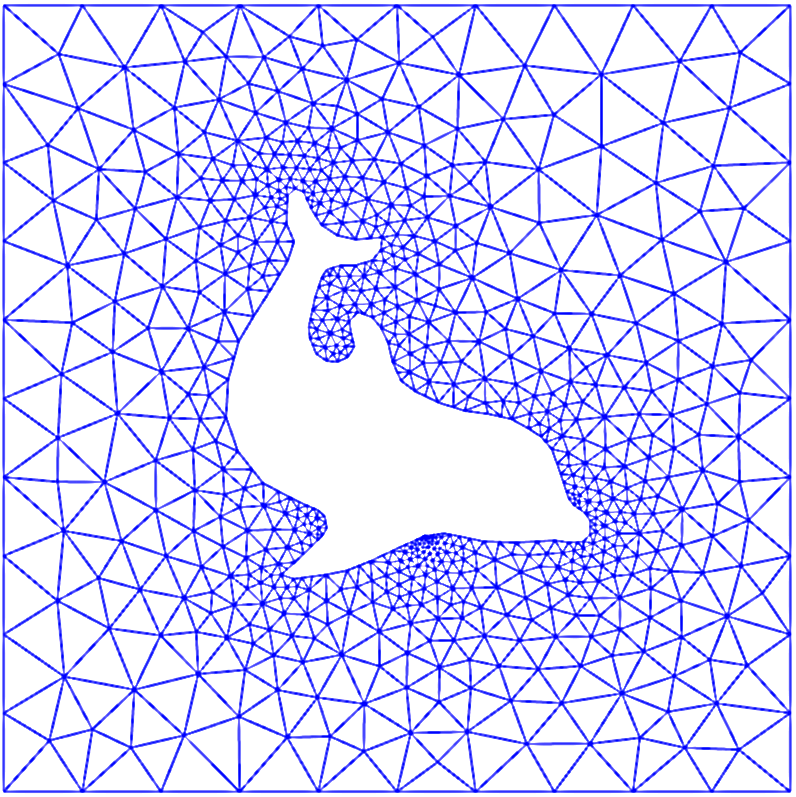
\includegraphics[width=\smallfig]{chapters/logg-2/png/plot_mesh.png}
  \caption{Plotting a mesh using the DOLFIN \emp{plot} command, here
    the mesh \emp{dolfin-1.xml.gz} distributed with DOLFIN.}
    \label{fig:logg-2:plots,mesh}
\end{figure}

\begin{figure}
\bwfig
\centering
  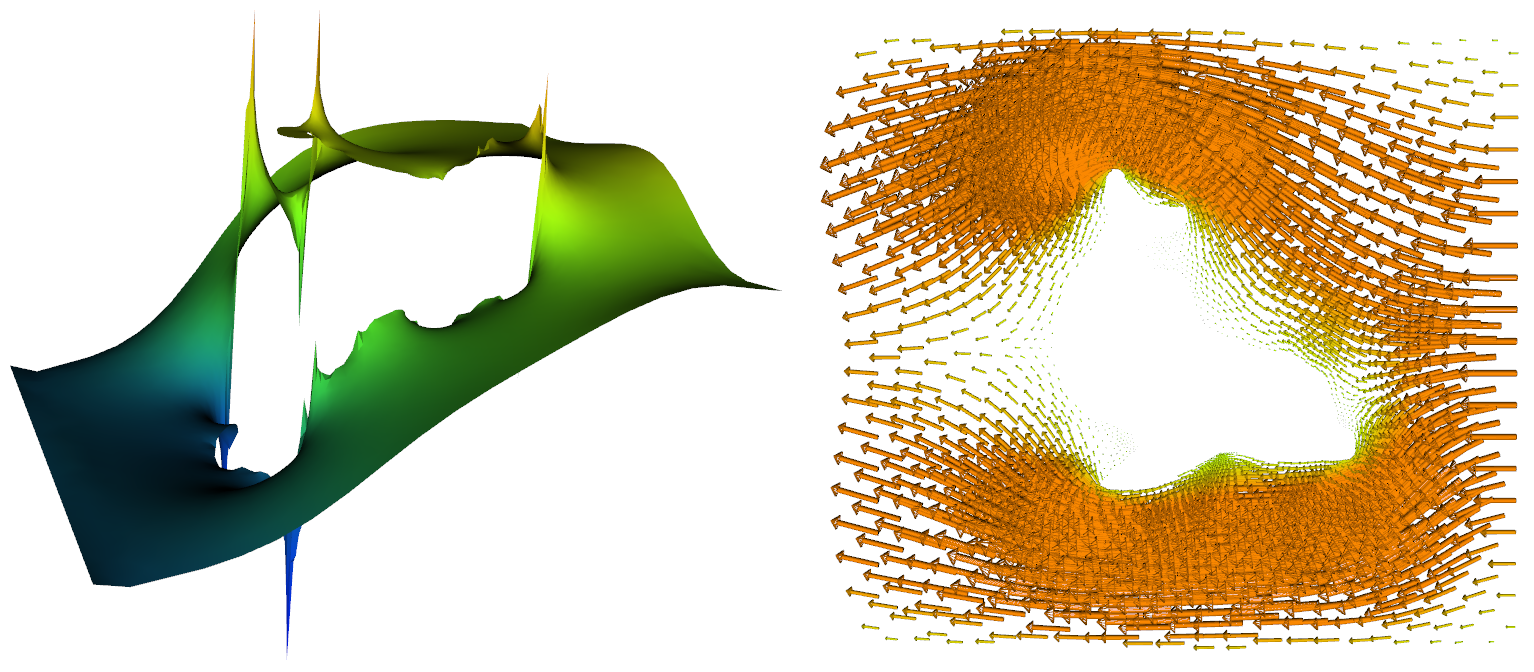
\includegraphics[width=\largefig]{chapters/logg-2/png/plots.png}
    \caption{Plotting a scalar and a vector-valued function using the
    DOLFIN \emp{plot} command, here the pressure (left) and velocity
    (right) from a solution of the Stokes equations on the mesh from
    Figure~\ref{fig:logg-2:plots,mesh}.}
  \label{fig:logg-2:plots,function}
\end{figure}

To enable interaction with a plot window (rotate, zoom) from Python,
call the function \emp{interactive}, or add an optional argument
\emp{interactive=True} to the \emp{plot} command.

\index{ParaView}
\index{MayaVi}
\index{file formats!PVD}
\index{file formats!VTU}

The \emp{plot} command provides rudimentary plotting, and advanced
postprocessing is better handled by external software such as
\citet{www:paraview} and \citet{www:mayavi}. This is easily
accomplished by storing the solution (a \emp{Function} object) to file
in PVD format (ParaView Data, an XML-based format). This can be done
in both C++ and Python by writing to a file with the \emp{.pvd}
extension, as illustrated in the following code examples:
%%
\begin{c++}
File file("solution.pvd");
file << u;
\end{c++}
\pagebreak
\begin{python}
file = File("solution.pvd")
file << u
\end{python}
%%
The standard PVD format is ASCII based, hence the file size can
become very large for large data sets. To use a compressed binary
format, a string \emp{"compressed"} can be used when creating a
PVD-based \emp{File} object:
%%
\begin{c++}
File file("solution.pvd", "compressed");
\end{c++}
%%
If multiple \emp{Function}s are written to the same file (by repeated
use of \emp{<{}<}), then the data is interpreted as a time series,
which may then be animated in ParaView or MayaVi2. Each frame of the
time series is stored as a \emp{.vtu} (VTK unstructured data) file,
with references to these files stored in the \emp{.pvd} file.  When
writing time-dependent data, it can be useful to store the time
\emp{t} of each snapshot. This is done as illustrated below:
%%
\begin{c++}
File file("solution.pvd", "compressed");
file << std::make_pair<const Function*, double>(&u, t);
\end{c++}
%%
\begin{python}
file = File("solution.pvd", "compressed");
file << (u, t)
\end{python}
%%
Storing the time is particularly useful when animating simulations that
use a varying time step.

The PVD format supports parallel post-processing. When running in
parallel, a single \emp{.pvd} file is created and a \emp{.vtu} file is
created for the data on each partition. Results computed in parallel
can be viewed seamlessly using ParaView.

\paragraph{DOLFIN XML format.}
\index{file formats!DOLFIN XML}

DOLFIN XML is the native format of DOLFIN. An advantage of XML is that
it is a robust and human-readable format. If the files are compressed,
there is also little overhead in terms of file size compared to a
binary format.

Many of the classes in DOLFIN can be written to and from DOLFIN XML
files using the standard stream operators \emp{<{}<} and \emp{>{}>}, as
illustrated in the following code examples:
%%
\begin{c++}
File vector_file("vector.xml");
vector_file << vector;
vector_file >> vector;

File mesh_file("mesh.xml");
mesh_file << mesh;
mesh_file >> mesh;

File parameters_file("parameters.xml");
parameters_file << parameters;
parameters_file >> parameters;
\end{c++}
%%
\begin{python}
vector_file = File("vector.xml")
vector_file << vector
vector_file >> vector

mesh_file = File("mesh.xml")
mesh_file << mesh
mesh_file >> mesh

parameters_file = File("parameters.xml")
parameters_file << parameters
parameters_file >> parameters
\end{python}
%%
One cannot read/write \emp{Function} and \emp{FunctionSpace} objects
since the representation of a\break \emp{FunctionSpace} (and thereby the
representation of a \emp{Function}) relies on generated code.

DOLFIN automatically handles reading and writing of gzipped XML files. Thus,
one may save space by storing meshes and other data in gzipped XML files
(with suffix \emp{.xml.gz}).

\paragraph{Time series.}
\index{time series}
\index{\emp{TimeSeries}}

For time-dependent problems, it may be useful to store a
sequence of solutions or meshes in a format that enables fast
reading/writing of data. For this purpose, DOLFIN provides the
\emp{TimeSeries} class. This enables the storage of a series of
\emp{Vector}s (of degrees of freedom) and/or \emp{Mesh}es. The
following code illustrates how to store a series of \emp{Vector}s and
\emp{Mesh}es to a \emp{TimeSeries}:
%%
\begin{c++}
TimeSeries time_series("simulation_data");

while (t < T)
{
  ...
  time_series.store(u.vector(), t);
  time_series.store(mesh, t);
  t += dt;
}
\end{c++}
%
\begin{python}
time_series = TimeSeries("simulation_data")

while t < T:
    ...
    time_series.store(u.vector(), t)
    time_series.store(mesh, t)
    t += dt
\end{python}
%%
Data in a \emp{TimeSeries} are stored in a binary format with one file
for each stored dataset (\emp{Vector} or \emp{Mesh}) and a common
index. Data may be retrieved from a \emp{TimeSeries} by calling the
\emp{retrieve} member function as illustrated in the code examples
below. If a dataset is not stored at the requested time, then the
values are interpolated linearly for \emp{Vector}s. For \emp{Mesh}es,
the closest data point will be used.
%%
\begin{c++}
time_series.retrieve(u.vector(), t);
time_series.retrieve(mesh, t);
\end{c++}
%%
\begin{python}
time_series.retrieve(u.vector(), t)
time_series.retrieve(mesh, t)
\end{python}

%------------------------------------------------------------------------------
\subsection{Logging / diagnostics}
\index{logging}

DOLFIN provides a simple interface for the uniform handling of log
messages, including warnings and errors. All messages are collected to a
single stream, which allows the destination and formatting of the output
from an entire program, including the DOLFIN library, to be controlled
by the user.

\paragraph{Printing messages.}
\index{\emp{info}}
\index{\emp{cout}}
\index{\emp{endl}}

Informational messages from DOLFIN are normally printed using the
\emp{info} command. This command takes a string argument and an
optional list of variables to be formatted, much like the standard
C \emp{printf} command. Note that the \emp{info} command
automatically appends a newline to the given string. Alternatively,
C++ users may use the \emp{dolfin::cout} and \emp{dolfin::endl} objects
for C++ style formatting of messages as illustrated below.
%%
\begin{c++}
info("Assembling system of size %d x %d.", M, N);
cout << "Assembling system of size " << M << " x " << N << "." << endl;
\end{c++}
%%
\begin{python}
info("Assembling system of size %d x %d." % (M, N))
\end{python}
%%
The \emp{info} command and the \emp{dolfin::cout/endl} objects differ
from the standard C \emp{printf} command and the C++
\emp{std::cout/endl} objects in that the output is directed into a
special stream, the output of which may be redirected to destinations
other than standard output. In particular, one may completely disable
output from DOLFIN, or select the verbosity of printed messages, as
explained below.

\paragraph{Warnings and errors.}
\index{\emp{warning}}
\index{\emp{error}}
\index{log level}

In addition to the \emp{info} command, DOLFIN provides the
commands \emp{warning} and \emp{error} that can be used to issue
warnings and errors, respectively. These two commands work in much the
same way as the \emp{info} command. However, the \emp{warning} command
will prepend the given message with \emp{"*** Warning: "} and the
\emp{error} command will raise an exception that can be caught, from
both C++ and Python. Both commands will also print the message at a
\emph{log level} higher than messages printed using \emp{info}.

\paragraph{Setting the log level.}
\index{\emp{set\_log\_level}}
\index{\emp{set\_log\_active}}

The DOLFIN log level determines which messages routed through the
logging system will be printed. Only messages on a level higher than
or equal to the current log level are printed. The log level of DOLFIN
may be set using the function \emp{set\_log\_level}. This function
expects an integer value that specifies the log level. To simplify the
specification of the log level, one may use one of a number of
predefined log levels as listed in Table~\ref{tab:logg-2:loglevels}. The default log
level is \emp{INFO}. Log messages may be switched off entirely by
calling the command \emp{set\_log\_active(false)} from C++ and
\emp{set\_log\_active(False)} from Python. For technical reasons, the
log level for debugging messages is named \emp{DBG} in C++ and
\emp{DEBUG} in Python. This is summarized in
Table~\ref{tab:logg-2:loglevels}.

\begin{table}
  \centering
  \begin{tabular}{cc}
    \toprule
    Log level & value \\
    \midrule
    \emp{ERROR} & \emp{40} \\
    \emp{WARNING} & \emp{30} \\
    \emp{INFO} & \emp{20} \\
    \emp{PROGRESS} & \emp{16} \\
    \emp{DBG} / \emp{DEBUG} & \emp{10} \\
    \bottomrule
  \end{tabular}
  \caption{Log levels in DOLFIN.}
  \label{tab:logg-2:loglevels}
\end{table}

To print messages at an arbitrary log level, one may specify the log
level to the \emp{log} command, as illustrated in the
code examples below.
%%
\begin{c++}
info("Test message");                      // will be printed
cout << "Test message" << endl;            // will be printed
log(DBG, "Test message");                  // will not be printed
log(15, "Test message");                   // will not be printed

set_log_level(DBG);
info("Test message");                      // will be printed
cout << "Test message" << endl;            // will be printed
log(DBG, "Test message");                  // will be printed
log(15, "Test message");                   // will be printed

set_log_level(WARNING);
info("Test message");                      // will not be printed
cout << "Test message" << endl;            // will not be printed
warning("Test message");                   // will be printed
std::cout << "Test message" << std::endl;  // will be printed!
\end{c++}
%%
\begin{python}
info("Test message")                       # will be printed
log(DEBUG, "Test message")                 # will not be printed
log(15, "Test message")                    # will not be printed

set_log_level(DEBUG)
info("Test message")                       # will be printed
log(DEBUG, "Test message")                 # will be printed
log(15, "Test message")                    # will be printed

set_log_level(WARNING)
info("Test message")                       # will not be printed
warning("Test message")                    # will be printed
print "Test message"                       # will be printed!
\end{python}

\paragraph{Printing objects.}

Many of the standard DOLFIN objects can be printed using the \emp{info}
command, as illustrated in the code examples below.
%%
\begin{c++}
info(vector);
info(matrix);
info(solver);
info(mesh);
info(mesh_function);
info(function);
info(function_space);
info(parameters);
\end{c++}
%%
\begin{python}
info(vector)
info(matrix)
info(solver)
info(mesh)
info(mesh_function)
info(function)
info(function_space)
info(parameters)
\end{python}
%%
The above commands will print short informal messages. For example,
the command \emp{info(mesh)} may result in the following output:
%%
\begin{gencode}
<Mesh of topological dimension 2 (triangles) with 25 vertices and 32 cells, ordered>
\end{gencode}
%%
In the Python interface, the same short informal message can be printed
by calling \emp{print mesh}. To print more detailed data, one may
set the verbosity argument of the \emp{info} function to true (defaults
to false), which will print a detailed summary of the object.
%%
\begin{c++}
info(mesh, true);
\end{c++}
%%
\begin{python}
info(mesh, True)
\end{python}
%%
The detailed output for some objects may be very lengthy.

\paragraph{Tasks and progress bars.}
\index{progress bar}
\index{\emp{begin}}
\index{\emp{end}}
\index{\emp{Progress}}

In addition to basic commands for printing messages, DOLFIN provides a
number of commands for organizing the diagnostic output from a simulation
program. Two such commands are \emp{begin} and \emp{end}. These commands
can be used to nest the output from a program; each call to \emp{begin}
increases the indentation level by one unit (two spaces), while each
call to \emp{end} decreases the indentation level by one unit.

Another way to provide feedback is via progress bars. DOLFIN provides
the \emp{Progress} class for this purpose. Although an effort has been
made to minimize the overhead of updating the progress bar, it should
be used with care. If only a small amount of work is performed in each
iteration of a loop, the relative overhead of using a progress bar
may be substantial. The code examples below illustrate the use of the
\emp{begin}/\emp{end} commands and the progress bar.
%%
\begin{c++}
begin("Starting nonlinear iteration.");
info("Updating velocity.");
info("Updating pressure.");
info("Computing residual.");
end();

Progress p("Iterating over all cells.", mesh.num_cells());
for (CellIterator cell(mesh); !cell.end(); ++cell)
{
  ...
  p++;
}

Progress q("Time-stepping");
while (t < T)
{
  ...
  t += dt;
  q = t / T;
}
\end{c++}
%%
\begin{python}
begin("Starting nonlinear iteration.")
info("Updating velocity.")
info("Updating pressure.")
info("Computing residual.")
end()

p = Progress("Iterating over all cells.", mesh.num_cells())
for cell in cells(mesh):
  ...
  p += 1

q = Progress("Time-stepping")
while t < T:
  ...
  t += dt
  q.update(t / T)
\end{python}

\paragraph{Setting timers.}
\index{timing}
\index{\emp{Timer}}

Timing can be accomplished using the \emp{Timer} class. A \emp{Timer} is
automatically started when it is created, and automatically stopped when
it goes out of scope. Creating a \emp{Timer} at the start of a function
is therefore a convenient way to time that function, as illustrated in
the code examples below.
%%
\begin{c++}
void solve(const Matrix& A, Vector& x, const Vector& b)
{
  Timer timer("Linear solve");
  ...
}
\end{c++}
%%
\begin{python}
def solve(A, b):
  timer = Timer("Linear solve")
  ...
  return x
\end{python}
%%
One may explicitly call the \emp{start} and \emp{stop} member
functions of a \emp{Timer}. To directly access the value of a timer,
the \emp{value} member function can be called. A summary of the
values of all timers created during the execution of a program can be
printed by calling the \emp{list\_timings} function.

%------------------------------------------------------------------------------
\subsection{Parameters}
\index{parameters}
\index{\emp{Parameters}}

DOLFIN keeps a global database of parameters that control the behavior
of its various components. Parameters are controlled via a uniform
type-independent interface that allows the retrieval of parameter
values, modification of parameter values, and the addition of new
parameters to the database. Different components (classes) of DOLFIN
also rely on parameters that are local to each instance of the class.
This permits different parameter values to be set for different
objects of a class.

Parameter values can be either integer-valued, real-valued (standard
double), string-valued or boolean-valued. Parameter
names must not contain spaces.

\paragraph{Accessing parameters.}

Global parameters can be accessed through the global variable
\emp{parameters}. The below code illustrates how to print the values of
all parameters in the global parameter database, and how to access and
change parameter values.
%%
\begin{c++}
info(parameters, True);
uint num_threads = parameters["num_threads"];
bool allow_extrapolation = parameters["allow_extrapolation"];
parameters["num_threads"] = 8;
parameters["allow_extrapolation"] = true;
\end{c++}
%%
\begin{python}
info(parameters, True)
num_threads = parameters["num_threads"]
allow_extrapolation = parameters["allow_extrapolation"]
parameters["num_threads"] = 8
parameters["allow_extrapolation"] = True
\end{python}
%%
Parameters that are local to specific components of DOLFIN can be
controlled by accessing the member variable named \emp{parameters}. The
following code illustrates how to set some parameters for a Krylov solver:
%%
\begin{c++}
KrylovSolver solver;
solver.parameters["absolute_tolerance"] = 1e-6;
solver.parameters["report"] = true;
solver.parameters("gmres")["restart"] = 50;
solver.parameters("preconditioner")["reuse"] = true;
\end{c++}
%%
\begin{python}
solver = KrylovSolver()
solver.parameters["absolute_tolerance"] = 1e-6
solver.parameters["report"] = True
solver.parameters["gmres"]["restart"] = 50
solver.parameters["preconditioner"]["reuse"] = True
\end{python}
%%
The above example accesses the nested parameter databases \emp{"gmres"}
and \emp{"preconditioner"}. DOLFIN parameters may be nested to
arbitrary depths, which helps with organizing parameters into different
categories. Note the subtle difference in accessing nested parameters in
the two interfaces. In the C++ interface, nested parameters are accessed
by brackets \emp{("...")}, and in the Python interface are they accessed
by square brackets \emp{["..."]}. The parameters that are available for
a certain component can be viewed by using the \emp{info} function.

\paragraph{Adding parameters.}

Parameters can be added to an existing parameter database using the
\emp{add} member function which takes the name of the new parameter
and its default value. It is also simple to create new parameter
databases by creating a new instance of the \emp{Parameters}
class. The following code demonstrates how to create a new parameter
database and adding to it a pair of integer-valued and floating-point
valued parameters:
%%
\begin{c++}
Parameters parameters("my_parameters");
my_parameters.add("foo", 3);
my_parameters.add("bar", 0.1);
\end{c++}
%%
\begin{python}
my_parameters = Parameters("my_parameters")
my_parameters.add("foo", 3)
my_parameters.add("bar", 0.1)
\end{python}
%%
A parameter database resembles the \emp{dict} class in the Python
interface. A user can iterate over the \emp{keys}, \emp{values} and
\emp{items}:
%%
\begin{python}
for key, value in parameters.items():
    print key, value
\end{python}
%%
A Python \emp{dict} can also be used to update a Parameter
database:
%%
\begin{python}
d = dict(num_threads=4, krylov_solver=dict(absolute_tolerance=1e-6))
parameters.update(d)
\end{python}
%%
A parameter database can also be created in more compact way in the
Python interface:
%%
\begin{python}
my_parameters = Parameters("my_parameters", foo=3, bar=0.1,
                           nested=Parameters("nested", baz=True))
\end{python}

\paragraph{Parsing command-line parameters.}

Command-line parameters may be parsed into the global parameter database
or into any other parameter database. The following code illustrates
how to parse command-line parameters in C++ and Python, and how to pass
command-line parameters to the program:
%%
\begin{c++}
int main(int argc, char* argv[])
{
  ...
  parameters.parse(argc, argv);
  ...
}
\end{c++}
%%
\begin{python}
parameters.parse()
\end{python}
%%
\begin{bash}
python myprogram.py --num_threads 8 --allow_extrapolation true
\end{bash}

\paragraph{Storing parameters to file.}

It can be useful to store parameter values to file, for example to
document which parameter values were used to run a simulation or to
reuse a set of parameter values from a previous run. The following code
illustrates how to write and then read back parameter values to/from a
DOLFIN XML file:
%%
\begin{c++}
File file("parameters.xml");
file << parameters;
file >> parameters;
\end{c++}
%%
\begin{python}
file = File("parameters.xml")
file << parameters
file >> parameters
\end{python}
At startup, DOLFIN automatically scans the current directory and the
directory \emp{.config/fenics} in the user's home directory (in that
order) for a file named \emp{dolfin\_parameters.xml}. If found, these
parameters are read into DOLFIN's global parameter database.

%------------------------------------------------------------------------------
%------------------------------------------------------------------------------
\section{Implementation notes}
\label{sec:logg-2:implementation}

In this section, we comment on specific aspects of the implementation
of DOLFIN, including parallel computing, the generation of the Python
interface, and just-in-time compilation.

%------------------------------------------------------------------------------
\subsection{Parallel computing}
\index{parallel computing}

DOLFIN supports parallel computing on multi-core workstations through
to massively parallel supercomputers. It is designed such that users
can perform parallel simulations using the same code that is used for
serial computations.

Two paradigms for parallel simulation are supported.  The first
paradigm is multithreading for shared memory machines.  The second
paradigm is fully distributed parallelization for distributed memory
machines. For both paradigms, special preprocessing of a mesh is
required.  For multithreaded parallelization, a so-called coloring
approach is used (see Figure~\ref{fig:logg-2:parallel}a), and for
distributed parallelization a mesh partitioning approach is used (see
Figure~\ref{fig:logg-2:parallel}b). Aspects of these two approaches are
discussed below. It is also possible to combine the approaches, thereby
yielding hybrid approaches to leverage the power of modern clusters of
multi-core processors.

\begin{figure}
  \centering
  \begin{tabular}{cc}
    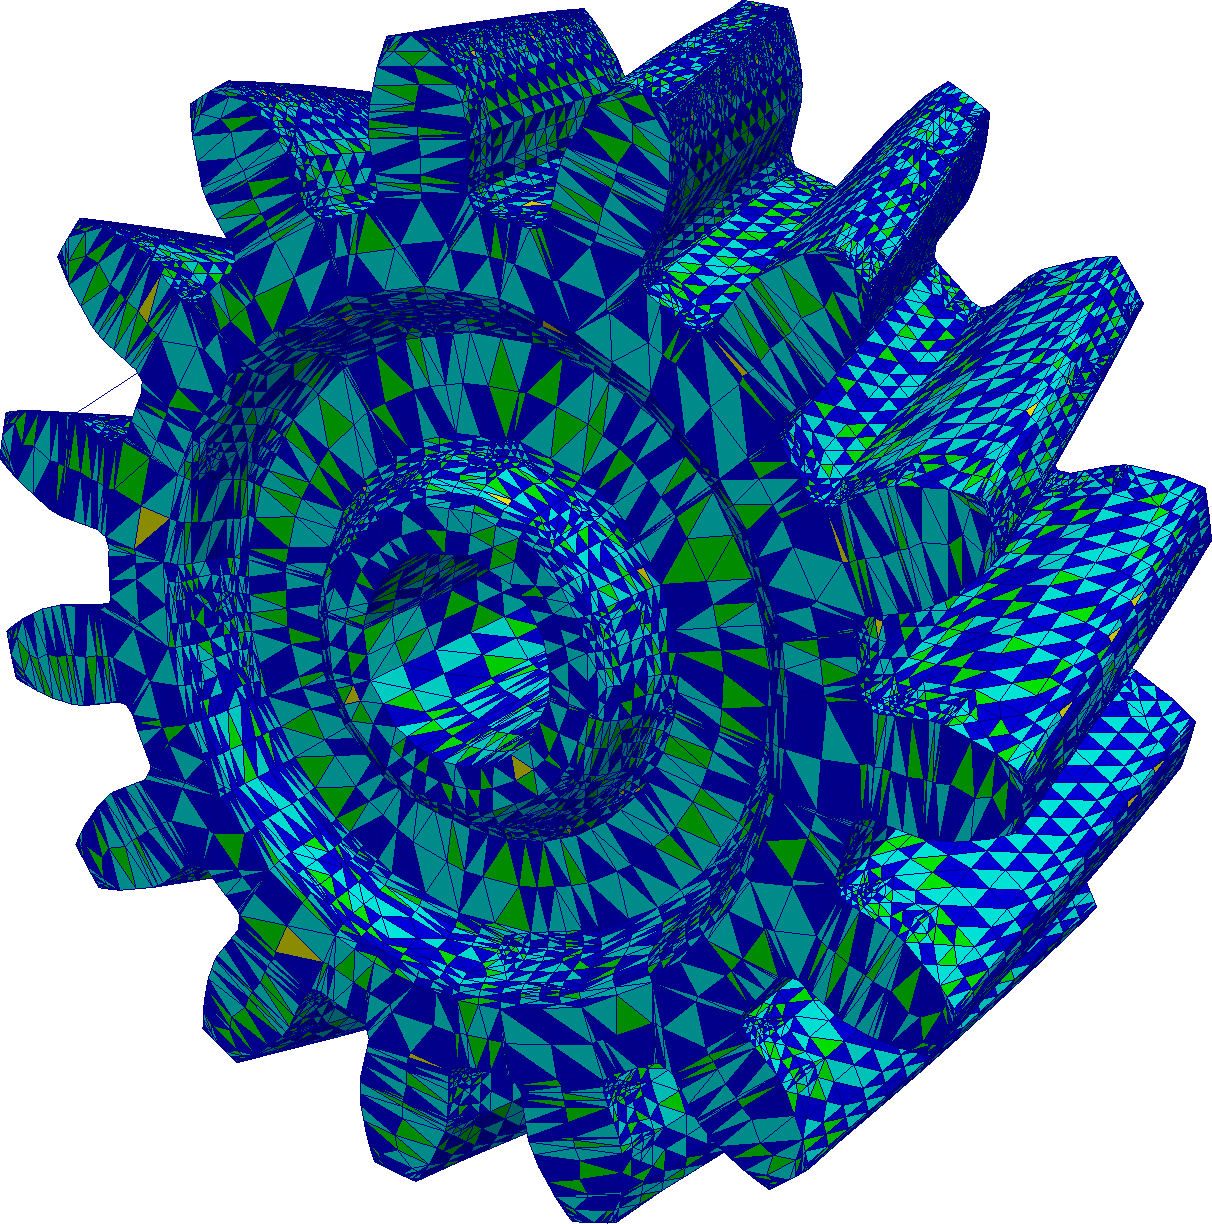
\includegraphics[width=\twofigs]{chapters/logg-2/png/coloured.png}
    &
    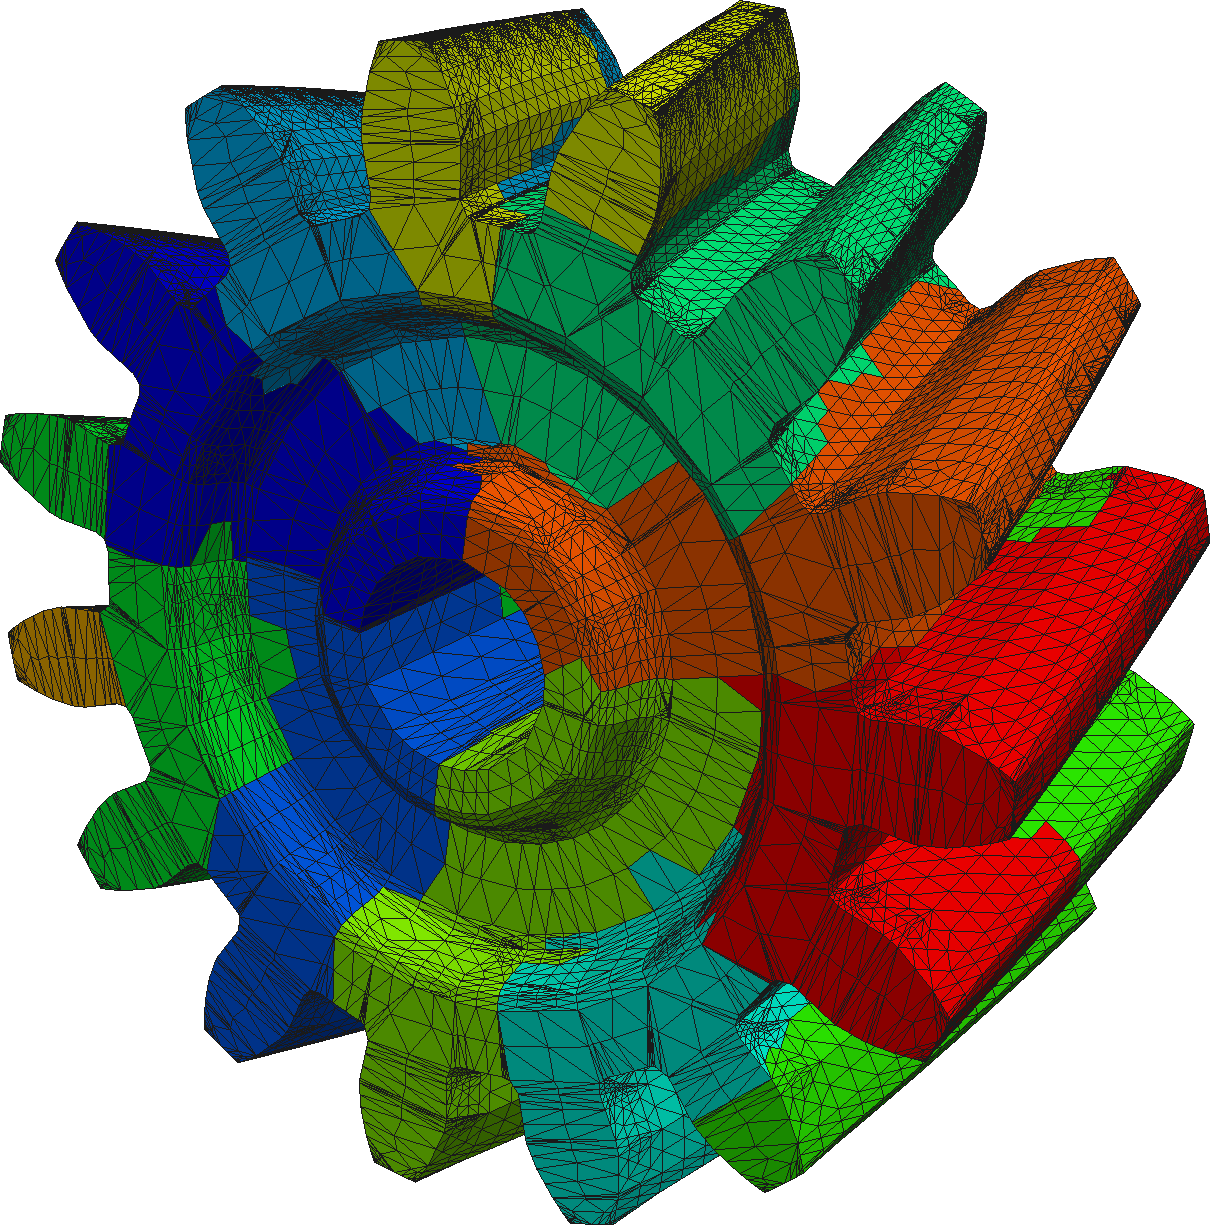
\includegraphics[width=\twofigs]{chapters/logg-2/png/partition.png}
    \\[1ex] (a) & (b)
  \end{tabular}
  \caption{A mesh that is (a) colored based on facet connectivity such
    that cells that share a common facet have different colors and
    (b) partitioned into 12 parts, with each partition indicated by
    a color.}
  \label{fig:logg-2:parallel}
\end{figure}

%------------------------------------------------------------------------------
\paragraph{Shared memory parallel computing.}
\index{parallel computing!shared memory}
\index{multicore}
\index{multithreading}
\index{mesh!coloring}

Multithreaded assembly for finite element matrices and vectors on shared
memory machines is supported using OpenMP. It is activated by
setting the number of threads to use via the parameter system.
For example, the code
%%
\begin{c++}
parameters["num_threads"] = 6;
\end{c++}
%%
\looseness-1{}instructs DOLFIN to use six threads in the assembly process.  During
assembly, DOLFIN loops over the cells or cell facets in a mesh, and
computes local contributions to the global matrix or vector, which are
then added to the global matrix or vector. When using multithreaded
assembly, each thread is assigned a collection of cells or facets for
which it is responsible. This is transparent to the user.

\enlargethispage{10pt}

The use of multithreading requires design care to avoid race conditions,
which occur if multiple threads attempt to write to the same memory
location at the same time.  Race conditions will typically result in
unpredictable behavior of a program. To avoid race conditions during
assembly, which would occur if two threads were to add values to a global
matrix or vector at almost the same time, DOLFIN uses a graph coloring
approach.  Before assembly, the mesh on a given process is `colored'
such that each cell is assigned a color (which in practice is an integer)
and such that no two neighboring cells have the same color. The sense
in which cells are neighbors for a given problem depends on the type
of finite element being used. In most cases, cells that share a vertex
are considered neighbors, but in other cases cells that share edges or
facets may be considered neighbors. During assembly, cells are assembled
by color. All cells of the first color are shared among the threads
and assembled, and this is followed by the next color. Since cells of
the same color are not neighbors, and therefore do not share entries in the
global matrix or vector, race conditions will not occur during assembly.
The coloring of a mesh is performed in DOLFIN using either the interface
to the Boost Graph Library or the interface to Zoltan (which is part of
the Trilinos project).  Figure~\ref{fig:logg-2:parallel}a shows a mesh
that has been colored such that no two neighboring cells (in the sense
of a shared facet) are of the same color.

Multithreaded support in third-party linear algebra libraries is limited
at the present time, but is an area of active development.  The LU solver
\citet{www:pastix}, which can be accessed via the PETSc linear algebra
backend, supports multithreaded parallelism.

%------------------------------------------------------------------------------
\paragraph{Distributed memory parallel computing.}
\index{parallel computing!distributed memory}
\index{MPI}
\index{mesh!partitioning}

Fully distributed parallel computing is supported using the Message
Passing Interface (MPI). To perform parallel simulations, DOLFIN should
be compiled with MPI and a parallel linear algebra backend (such as PETSc
or Trilinos) enabled. To execute a parallel simulation, a DOLFIN program
should be launched using \emp{mpirun} (the name of the program to launch MPI
programs may differ on some computers). A C++ program using 16 processes
can be executed using:
%%
\begin{bash}
mpirun -n 16 ./myprogram
\end{bash}
%%
and for Python:
%%
\begin{bash}
mpirun -n 16 python myprogram.py
\end{bash}

\index{SCOTCH}
\index{ParMETIS}

DOLFIN supports fully distributed parallel meshes, which means that each
processor has a copy of only the portion of the mesh for which it is
responsible. This approach is scalable since no processor is required
to hold a copy of the full mesh.
An important step in a parallel simulation is the partitioning of the
mesh. DOLFIN can perform mesh partitioning in parallel using the libraries
\citet{www:parmetis} and SCOTCH \citep{www:scotch}.  The library to be
used for mesh partitioning can be specified via the parameter system,
e.g., to use SCOTCH:
%%
\begin{c++}
parameters["mesh_partitioner"] = "SCOTCH";
\end{c++}
%%
or to use ParMETIS:
%%
\begin{python}
parameters["mesh_partitioner"] = "ParMETIS"
\end{python}
%%
Figure~\ref{fig:logg-2:parallel}b shows a mesh that has been partitioned
in parallel into 12 domains. One process would take responsibility
for each domain.

If a parallel program is launched using MPI and a parallel linear
algebra backend is enabled, then linear algebra operations will be
performed in parallel. In most applications, this will be transparent
to the user.  Parallel output for postprocessing is supported through
the PVD output format, and is used in the same way as for serial
output. Each process writes an output file, and the single main output
file points to the files produced by the different processes.

%------------------------------------------------------------------------------
\subsection{Implementation and generation of the Python interface}

The DOLFIN C++ library is wrapped to Python using the Simplified
Wrapper and Interface Generator \swig \citep{Beazley2006,www:swig};
see Chapter~\ref{chap:mardal-2} for more details. The wrapped C++
library is accessible in a Python module named \emp{cpp} residing inside the
main \emp{dolfin} module of DOLFIN. This means that the compiled
module, with all its functions and classes, can be accessed directly
by:
%%
\begin{python}
from dolfin import cpp
Function = cpp.Function
assemble = cpp.assemble
\end{python}
%%
The classes and functions in the \emp{cpp} module have the same
functionality as the corresponding classes and functions in the C++
interface. In addition to the wrapper layer automatically generated
by SWIG, the DOLFIN Python interface relies on a number of components
implemented directly in Python. Both are imported into the Python module
named \emp{dolfin}. In the following sections, the key customizations to
the DOLFIN interface that facilitate this integration are presented. The
Python interface also integrates well with the \numpy and \scipy toolkits,
which is also discussed below.

%------------------------------------------------------------------------------
\subsection{UFL integration and just-in-time compilation}

In the Python interface, the UFL form language has been integrated
with the Python wrapped DOLFIN C++ module.  When explaining the
integration, we use in this section the notation \emp{dolfin::Foo}
or \emp{dolfin::bar} to denote a C++ class or function in \dolfin. The
corresponding \swig-wrapped classes or functions will be referred to
as \emp{cpp.Foo} and \emp{cpp.bar}. A class in UFL will be referred
to as \emp{ufl.Foo} and a class in \ufc as \emp{ufc::foo} (note lower
case). The Python classes and functions in the added Python layer on
top of the wrapped C++ library, will be referred to as \emp{dolfin.Foo}
or \emp{dolfin.bar}. The prefixes of the classes and functions are
sometimes skipped for convenience. Most of the code snippets presented
in this section are pseudo code. Their purpose is to illustrate the
logic of a particular method or function. Parts of the actual code may
be intentionally excluded. An interested reader can examine particular classes or
functions in the code for a full understanding of the implementation.

\paragraph{Construction of function spaces.}
In the Python interface, \emp{ufl.FiniteElement} and
\emp{dolfin::Function-\break Space} are integrated. The declaration of a
\emp{FunctionSpace} is similar to that of a \emp{ufl.FiniteElement},
but instead of a cell type (for example, \emp{triangle}) the
\emp{FunctionSpace} constructor takes a \emp{cpp.Mesh} (\emp{dolfin.Mesh}):
%%
\begin{python}
mesh = UnitSquare(8, 8)
V = FunctionSpace(mesh, "Lagrange", 1)
\end{python}
%%
In the Python constructor of \emp{FunctionSpace}, a
\emp{ufl.FiniteElement} is instantiated. The \emp{FiniteElement}
is passed to a just-in-time (JIT) compiler, which returns compiled
and Python-wrapped \emp{ufc} objects: a \emp{ufc::finite\_element}
and a \emp{ufc::dofmap}. These two objects, together with the mesh,
are used to instantiate a \emp{cpp.FunctionSpace}. The following pseudo
code illustrates the instantiation of a \emp{FunctionSpace} from the
Python interface:
%%
\begin{python}
class FunctionSpace(cpp.FunctionSpace):
    def __init__(self, mesh, family, degree):
        # Figure out the domain from the mesh topology
        if mesh.topology().dim() == 2:
            domain = ufl.triangle
        else:
            domain = ufl.tetrahedron

        # Create the UFL FiniteElement
        self.ufl_element = ufl.FiniteElement(family, domain, degree)

        # JIT compile and instantiate the UFC classes
        ufc_element, ufc_dofmap = jit(self.ufl_element)

        # Instantiate DOLFIN classes and finally the FunctionSpace
        dolfin_element = cpp.FiniteElement(ufc_element)
        dolfin_dofmap = cpp.DofMap(ufc_dofmap, mesh)
        cpp.FunctionSpace.__init__(self, mesh, dolfin_element, dolfin_dofmap)
\end{python}

\paragraph{Constructing arguments (trial and test functions).}

The \emp{ufl.Argument} class (the base class of\break \emp{ufl.TrialFunction}
and \emp{ufl.TestFunction}) is subclassed in the Python interface. Instead
of using a \emp{ufl.FiniteElement} to instantiate the classes, a DOLFIN
\emp{FunctionSpace} is used:
%%
\begin{python}
u = TrialFunction(V)
v = TestFunction(V)
\end{python}
%%
The \emp{ufl.Argument} base class is instantiated in the subclassed
constructor by extracting the\break \emp{ufl.FiniteElement} from the passed
\emp{FunctionSpace}, which is illustrated by the following pseudo
code:
%%
\begin{python}
class Argument(ufl.Argument):
    def __init__(self, V, index=None):
        ufl.Argument.__init__(self, V.ufl_element, index)
        self.V = V
\end{python}
%%
The \emp{TrialFunction} and \emp{TestFunction} are then defined using the
subclassed \emp{Argument} class:
%%
\begin{python}
def TrialFunction(V):
    return Argument(V, -1)

def TestFunction(V):
    return Argument(V, -2)
\end{python}

\enlargethispage{12pt}

\paragraph{Coefficients, functions and expressions.}

When a UFL form is defined using a \emp{Coefficient}, a user must
associate with the form either a discrete finite element
\emp{Function} or a user-defined \emp{Expression} before the form is
assembled. In the C++ interface of DOLFIN, a user needs to explicitly
carry out this association (\emp{L.f = f}). In the Python interface of
DOLFIN, the \emp{ufl.Coefficient} class is combined with the \dolfin
\emp{Function} and \emp{Expression} classes, and the association
between the coefficient as a symbol in the form expression
(\emp{Coefficient}) and its value (\emp{Function} or \emp{Expression})
is automatic. A user can therefore assemble a form defined using
instances of these combined classes directly:
%%
\begin{python}
class Source(Expression):
    def eval(self, values, x):
        values[0] = sin(x[0])

v = TestFunction(V)
f = Source()
L = f*v*dx
b = assemble(L)
\end{python}
%%
The \emp{Function} class in the Python interface inherits from both
\emp{ufl.Coefficient} and \emp{cpp.Function}, as illustrated by the
following pseudo code:
%%
\begin{python}
class Function(ufl.Coefficient, cpp.Function):
    def __init__(self, V):
        ufl.Coefficient.__init__(self, V.ufl_element)
        cpp.Function().__init__(self, V)
\end{python}
%%
The actual constructor also includes logic to instantiate a \emp{Function}
from other objects. A more elaborate logic is also included to handle
access to subfunctions.

A user-defined \emp{Expression} can be created in two different ways:
(i)~as a pure Python \emp{Expression}; or (ii)~as a JIT compiled
\emp{Expression}. A pure Python \emp{Expression} is an object instantiated
from a subclass of \emp{Expression} in Python. The \emp{Source} class
above is an example of this. Pseudo code for the constructor of the
\emp{Expression} class is similar to that for the \emp{Function} class:
%%
\begin{python}
class Expression(ufl.Coefficient, cpp.Expression):
    def __init__(self, element=None):
        if element is None:
            element = auto_select_element(self.value_shape())
        ufl.Coefficient.__init__(self, element)
        cpp.Expression(element.value_shape())
\end{python}
%%
If the \emp{ufl.FiniteElement} is not defined by the user, DOLFIN will
automatically choose an element using the \emp{auto\_select\_element}
function. This function takes the value shape of the \emp{Expression}
as argument. This has to be supplied by the user for vector- or
tensor-valued \emp{Expression}s, by overloading the \emp{value\_shape}
method. The base class \emp{cpp.Expression} is initialized using the
value shape of the \emp{ufl.FiniteElement}.

\index{metaclass}

The actual code is considerably more complex than indicated above, as
the same class, \emp{Expression}, is used to handle both JIT compiled
and pure Python \emp{Expression}s. Also note that the actual subclass
is eventually generated by a \emph{metaclass} in Python, which makes it
possible to include sanity checks for the declared subclass.

The \emp{cpp.Expression} class is wrapped by a so-called \emph{director class} in
the \swig-generated C++ layer. This means that the whole Python class is
wrapped by a C++ subclass of \emp{dolfin::Expression}. Each virtual method
of the C++ base class is implemented by the \swig-generated subclass in
C++. These methods call the Python version of the method, which the user
eventually implements by subclassing \emp{cpp.Expression} in Python.

\paragraph{Just-in-time compilation of expressions.}
\index{just-in-time compilation}

The performance of a pure Python \emp{Expression} may be suboptimal
because of the callback from C++ to Python each time the \emp{Expression}
is evaluated. To circumvent this, a user can instead subclass the C++
version of \emp{Expression} using a JIT compiled \emp{Expression}. Because
the subclass is implemented in C++, it will not involve any callbacks
to Python, and can therefore be significantly faster than a pure Python
\emp{Expression}. A JIT compiled \emp{Expression} is generated by passing
a string of C++ code to the \emp{Expression} constructor:
%%
\begin{python}
e = Expression("sin(x[0])")
\end{python}
%%
The passed string is used to generate a subclass of
\emp{dolfin::Expression} in C++, where it is inlined into an overloaded
\emp{eval} method. The final code is JIT compiled and wrapped to Python
using \instant (see Chapter~\ref{chap:wilbers}). The generated Python
class is then imported into Python. The class is not yet instantiated,
as the final JIT compiled \emp{Expression} also needs to inherit from
\emp{ufl.Coefficient}. To accomplish this, we dynamically create a class
which inherits from both the generated class and \emp{ufl.Coefficient}.

Classes in Python can be created during run-time by using the
\emp{type} function. The logic of creating a class and returning an
instance of that class is handled in the \emp{\_\_new\_\_} method of
\emp{dolfin.Expression}, as illustrated by the following pseudo code:
\vspace*{16pt}\begin{python}
class Expression(object):
    def __new__(cls, cppcode=None):
        if cls.__name__ != "Expression":
            return object.__new__(cls)
        cpp_base = compile_expressions(cppcode)
        def __init__(self, cppcode):
            ...
        generated_class = type("CompiledExpression",
                               (Expression, ufl.Coefficient, cpp_base),
                               {"__init__": __init__})
        return generated_class()
\end{python}
%%
The \emp{\_\_new\_\_} method is called when a JIT compiled
\emp{Expression} is instantiated. However, it will also be called when
a pure Python subclass of \emp{Expression} is instantiated during
initialization of the base-class. We handle the two different cases by
checking the name of the instantiated class. If the name of the class
is not \emp{"Expression"}, then the call originates from the
instantiation of a subclass of \emp{Expression}. When a pure Python
\emp{Expression} is instantiated, like the \emp{Source} instance in
the code example above, the \emp{\_\_new\_\_} method of \emp{object}
is called and the instantiated object is returned.  In the other case,
when a JIT compiled \emp{Expression} is instantiated, we need to
generate the JIT compiled base class from the passed Python string, as
explained above. This is done by calling the function
\emp{compile\_expressions}. Before \emp{type} is called to generate
the final class, an \emp{\_\_init\_\_} method for the class is
defined. This method initiates the new object by automatically
selecting the element type and setting dimensions for the created
\emp{Expression}. This procedure is similar to what is done for the
Python derived \emp{Expression} class. Finally, we construct the new
class which inherits the JIT compiled class and \emp{ufl.Coefficient}
by calling \emp{type}.

The \emp{type} function takes three arguments: the name of the class
(\emp{"CompiledExpression"}), the bases of the class (\emp{Expression,
  ufl.Coefficient, cpp\_base}), and a \emp{dict} defining the
interface (methods and attributes) of the class. The only new method or
attribute we provide to the generated class is the \emp{\_\_init\_\_}
method. After the class is generated, we instantiate it and the object
is returned to the user.

\paragraph{Assembly of UFL forms.}

The \emp{assemble} function in the Python interface of DOLFIN enables
a user to directly assemble a declared UFL form:
%%
\begin{python}
mesh = UnitSquare(8, 8)
V = FunctionSpace(mesh, "Lagrange", 1)
u = TrialFunction(V)
v = TestFunction(V)
c = Expression("sin(x[0])")
a = c*dot(grad(u), grad(v))*dx
A = assemble(a)
\end{python}
%%
The \emp{assemble} function is a thin wrapper layer around the wrapped
\emp{cpp.assemble} function. The following pseudo code illustrates what
happens in this layer:
%%
\begin{python}
def assemble(form, tensor=None, mesh=None):
    dolfin_form = Form(form)
    if tensor is None:
        tensor = create_tensor(dolfin_form.rank())
    if mesh is not None:
        dolfin_form.set_mesh(mesh)
    cpp.assemble(dolfin_form, tensor)
    return tensor
\end{python}
%%
Here, \emp{form} is a \emp{ufl.Form}, which is used to generate a
\emp{dolfin.Form}, as explained below. In addition to the \emp{form}
argument, a user can choose to provide a tensor and/or a mesh. If a
tensor is not provided, one will automatically be generated by the
\emp{create\_tensor} function. The optional mesh is needed if the form
does not contain any \emp{Argument}s, or \emp{Function}s; for example
when a functional containing only \emp{Expression}s is assembled. Note
that the length of the above signature has been shortened. Other
arguments to the \emp{assemble} function exist but are skipped here
for clarity.

The following pseudo code demonstrates what happens in the constructor
of \emp{dolfin.Form}, where the base class \emp{cpp.Form} is initialized
from a \emp{ufl.Form}:
%%
\begin{python}
class Form(cpp.Form):
    def __init__(self, form):
        compiled_form, form_data = jit(form)
        function_spaces = extract_function_spaces(form_data)
        coefficients = extract_coefficients(form_data)
        cpp.Form.__init__(self, compiled_form, function_spaces, coefficients)
\end{python}
%%
The \emp{form} is first passed to the \emp{dolfin.jit} function,
which calls the registered form compiler to generate code and JIT
compile it. There are presently two form compilers that can be
chosen: \emp{"ffc"} and \emp{"sfc"} (see Chapters~\ref{chap:logg-1}
and~\ref{chap:alnes-3}). Each one of these form compilers defines its
own \emp{jit} function, which eventually will receive the call. The form
compiler can be chosen by setting:
%%
\begin{python}
parameters["form_compiler"]["name"] = "sfc"
\end{python}
%%
The default form compiler is \emp{"ffc"}. The \emp{jit} function of
the form compiler returns the JIT compiled \emp{ufc::form} together
with a \emp{ufl.FormData} object. The latter is a data structure
containing metadata for the \emp{ufl.form}, which is used to extract
the function spaces and coefficients that are needed to instantiate a
\emp{cpp.Form}. The extraction of these data is handled by the
\emp{extract\_function\_spaces} and the \emp{extract\_coefficients}
functions.

%------------------------------------------------------------------------------
\subsection{\numpy and \scipy integration}
\index{NumPy}
\index{SciPy}

The values of the \emp{Matrix} and \emp{Vector} classes in the Python
interface of DOLFIN can be viewed as \numpy arrays. This is done by
calling the \emp{array} method of the vector or matrix:
%%
\begin{python}
A  = assemble(a)
AA = A.array()
\end{python}
%%
Here, \emp{A} is a matrix assembled from the form \emp{a}. The \numpy
array \emp{AA} is a dense structure and all values are copied from the
original data. The \emp{array} function can be called on a distributed
matrix or vector, in which case it will return the locally stored
values.

% Removed comment about calling array on a distributed matrix. What
% it does is that it returns the submatrix for the rows stored on the
% local process by calling MatGetRow for those rows.

\paragraph{Direct access to linear algebra data.}

Direct access to the underlying data is possible for the uBLAS
and MTL4 linear algebra backends. A \numpy array view into the
data will be returned by the method \emp{data}:
%%
\begin{python}
parameters["linear_algebra_backend"] = "uBLAS"
b = assemble(L)
bb = b.data()
\end{python}
%%
Here, \emp{b} is a uBLAS vector and \emp{bb} is a \numpy view
into the data of \emp{b}. Any changes to \emp{bb} will directly affect
\emp{b}. A similar method exists for matrices:
%%
\begin{python}
parameters["linear_algebra_backend"] = "MTL4"
A = assemble(a)
rows, columns, values = A.data()
\end{python}
%%
The data is returned in a compressed row storage format as the three
\numpy arrays \emp{rows}, \emp{columns} and \emp{values}. These are also
views of the data that represent \emp{A}. Any changes in \emp{values}
will directly result in a corresponding change in~\emp{A}.

\paragraph{Sparse matrix and SciPy integration.}

The \emp{rows}, \emp{columns} and \emp{values} data structures can
be used to instantiate a \emp{csr\_matrix} from the \emp{scipy.sparse}
module \citep{JonesOliphantPetersonEtAl2009}:
%%
\begin{python}
from scipy.sparse import csr_matrix
rows, columns, values = A.data()
csr = csr_matrix((values, columns, rows))
\end{python}
%%
The \emp{csr\_matrix} can then be used with other Python modules
that support sparse matrices, such as the \emp{scipy.sparse}
module and \emp{pyamg}, which is an algebraic multigrid solver
\citep{BellOlsonSchroder2009}.

\paragraph{Slicing vectors.}

\numpy provides a convenient slicing interface for \numpy arrays. The
Python interface of DOLFIN also provides such an interface for vectors
(see Chapter~\ref{chap:mardal-2} for details of the implementation). A
slice can be used to access and set data in a vector:
%%
\begin{python}
# Create copy of vector
b_copy = b[:]

# Slice assignment (c can be a scalar, a DOLFIN vector or a NumPy array)
b[:] = c

# Set negative values to zero
b[b < 0] = 0

# Extract every second value
b2 = b[::2]
\end{python}
%%
A difference between a \numpy slice and a slice of a DOLFIN vector is
that a slice of a \numpy array provides a view into the original array,
whereas in DOLFIN we provide a copy. A list/tuple of integers or a \numpy
array can also be used to both access and set data in a vector:
%%
\begin{python}
b1 = b[[0, 4, 7, 10]]
b2 = b[array((0, 4, 7, 10))]
\end{python}

%------------------------------------------------------------------------------
%------------------------------------------------------------------------------
\section{Historical notes}

The first public version of DOLFIN, version~0.2.0, was released in
2002. At that time, DOLFIN was a self-contained C++ library with
minimal external dependencies. All functionality was then implemented
as part of DOLFIN itself, including linear algebra and finite element
form evaluation. Although only piecewise linear elements were
supported, DOLFIN provided rudimentary automated finite element
assembly of variational forms. The form language was implemented by
C++ operator overloading. For an overview of the development of the
FEniCS form language and an example of the early form language
implemented in DOLFIN, see Chapter~\ref{chap:logg-1}.

Later, parts of the functionality of DOLFIN have been moved to either
external libraries or other FEniCS components. In 2003, the FEniCS
project was born and shortly after, with the release of version~0.5.0 in
2004, the form evaluation system in DOLFIN was replaced by an automated
code generation system based on FFC and FIAT. In the following year,
the linear algebra was replaced by wrappers for PETSc data structures
and solvers. At this time, the DOLFIN Python interface ({Py}DOLFIN) was
introduced. Since then, the Python interface has developed from a simple
auto-generated wrapper layer for the DOLFIN C++ functionality to a mature
problem-solving environment with support for just-in-time compilation of
variational forms and integration with external Python modules like NumPy.

In 2006, the DOLFIN mesh data structures were simplified and
reimplemented to improve efficiency and expand functionality. The new
data structures were based on a light-weight object-oriented layer on
top of an underlying data storage by plain contiguous C/C++ arrays and
improved the efficiency by orders of magnitude over the old
implementation, which was based on a fully object-oriented
implementation with local storage of all mesh entities like cells and
vertices. The first release of DOLFIN with the new mesh library was
version~0.6.2.

In 2007, the UFC interface was introduced and the FFC form language was
integrated with the DOLFIN Python interface. Just-in-time compilation
was also introduced. The following year, the linear algebra interfaces
of DOLFIN were redesigned to allow flexible handling of multiple linear
algebra backends. In 2009, a major milestone was reached when parallel
computing was introduced in DOLFIN.

Over the years, DOLFIN has undergone a large number of changes to its
design, interface and implementation. However, since the release of
DOLFIN 0.9.0, which introduced a redesign of the DOLFIN function classes
based on the new function space abstraction, only minor changes have been
made to the interface. Since the release of version~0.9.0, most work has
gone into refining the interface, implementing missing functionality,
fixing bugs and improving documentation, in anticipation of the
first stable release of DOLFIN, version 1.0.

\enlargethispage{12pt}

% Used in algorithms
\newcommand{\afor}{\textbf{for} {}}
\newcommand{\aif}{\textbf{if} {}}
\newcommand{\aelse}{\textbf{else} {}}
\newcommand{\seq}[1]{\left\langle{#1}\right\rangle}

% Boldface letters
\renewcommand{\AA}{{A}}
\newcommand{\BB}{{B}}
\newcommand{\CC}{{C}}
\newcommand{\FF}{{F}}
\newcommand{\II}{{I}}
\newcommand{\MM}{{M}}
\newcommand{\PP}{{P}}
\renewcommand{\SS}{{S}}
\newcommand{\VV}{{V}}
\newcommand{\bb}{{b}}
\newcommand{\ee}{{e}}

\newcommand{\nn}{{n}}
\newcommand{\uu}{{u}}
\newcommand{\vv}{{v}}
\newcommand{\ww}{{w}}
\newcommand{\xx}{{x}}
\newcommand{\ff}{{f}}

\newcommand{\bpsi}{\bm{\psi}}
\newcommand{\bphi}{\bm{\phi}}
\newcommand{\bPsi}{\bm{\Psi}}
\newcommand{\bPhi}{\bm{\Phi}}

% Caligraphic letters
\newcommand{\mI}{\mathfrak{I}}

\newcommand{\Cc}{\mathcal{C}}
\newcommand{\Dc}{\mathcal{D}}
\newcommand{\Ic}{\mathcal{I}}

\newcommand{\mop}[1]{\operatorname{#1}}
\newcommand{\spans}[1]{\mop{span}\left\{ #1 \right\}}

%//////////////////////////////////////////////////////////////////////////////
\fenicschapter{UFL: a finite element form language}
              {UFL: a finite element form language}
              {UFL: a finite element form language}
              {Martin Sandve Aln\ae{}s}
              {alnes-1}
%\\\\\\\\\\\\\\\\\\\\\\\\\\\\\\\\\\\\\\\\\\\\\\\\\\\\\\\\\\\\\\\\\\\\\\\\\\\\\\

\index{Unified Form Language}
\index{\ufl{}}
\index{variational form}
\index{weak form}
\index{functional}
\index{form language}
\index{domain specific language}

The Unified Form Language -- \ufl{} \citep{AlnaesLogg2009} --
is a domain specific language for the declaration of finite element
discretizations of variational forms and functionals. More precisely,
the language defines a flexible user interface for defining finite
element spaces and expressions for weak forms in a notation close to
mathematical notation.

The \fenics{} project provides a framework for building applications
for solving partial differential equations (PDEs).  \ufl{} is one of
the core components of this framework.  It defines the language you
\emph{express} your PDEs in.  It is the input language and front-end
of the form compilers \ffc{} and \sfc{}, which are covered in
Chapter~\ref{chap:logg-1} and Chapter~\ref{chap:alnes-3}.  The \ufl{}
implementation also provides algorithms that the form compilers can
use to simplify the compilation process.  The output from these form
compilers is C++ \citep{Stroustrup1997} code that conforms to the \ufc{}
specification, which is explained in Chapter~\ref{chap:alnes-2}.
This code can be used with the C++/Python library \dolfin{}, which
is covered in Chapter~\ref{chap:logg-2}, to efficiently assemble
linear systems and compute solutions to PDEs.  Note that this chapter
does not cover how to actually solve equations defined in UFL. See
Chapter~\ref{chap:langtangen} for a tutorial on how to use the complete
\fenics{} framework to solve equations.

This chapter is intended both for the \fenics{} user who wants to
learn how to express her equations, and for other \fenics{} developers
and technical users who want to know how \ufl{} works on the inside.
Therefore, the sections of this chapter are organized with an
increasing amount of technical details.
Sections~\ref{ufl:sec:overview}--\ref{ufl:sec:formtransformations}
give an overview of the language as seen by the end-user and is
intended for all audiences.
Sections~\ref{ufl:sec:representation}--\ref{ufl:sec:implementation}
explain the design of the implementation and dive into some
implementation details.  Many details of the language have to be
omitted in a text such as this, and we refer to the \ufl{} manual
\citep{AlnaesLogg2009} for a more thorough description. Note that this
chapter refers to \ufl{} version 1.0.0, and both the user interface
and the implementation may change in future versions.

Starting with a brief overview, we mention the main design goals for
\ufl{} and show an example implementation of a non-trivial PDE in
Section~\ref{ufl:sec:overview}.  Next, we look at how to define finite
element spaces in Section~\ref{ufl:sec:elements}, followed by the
overall structure of forms and their declaration in
Section~\ref{ufl:sec:forms}.  The main part of the language is
concerned with defining expressions from a set of data types and
operators, which are discussed in Section~\ref{ufl:sec:defexpr}.
Operators applying to entire forms are the topic of
Section~\ref{ufl:sec:formtransformations}.

The technical part of the chapter begins with
Section~\ref{ufl:sec:representation} which discusses the
representation of expressions.  Building on the notation and
data structures defined there, how to compute derivatives is
discussed in Section~\ref{ufl:sec:ad}.  Some central internal
algorithms and key issues in their implementation are discussed in
Section~\ref{ufl:sec:algorithms}.  Implementation details, some of which
are specific to the programming language Python \citep{Rossumothers},
are the topic of Section~\ref{ufl:sec:implementation}.  Finally,
Section~\ref{ufl:sec:future} discusses future prospects of the \ufl{}
project.

%------------------------------------------------------------------------------
\subsection{Related work} \label{ufl:sec:related}

The combination of domain specific languages and symbolic computing
with finite element methods has been pursued from other angles in
several other projects.  Sundance \citep{Long2003,Long2004a,Long2004}
implements a symbolic engine directly in C++ to define variational
forms, and has support for automatic differentiation.  The Life
\citep{Prudhomme2006a,Prudhomme2006} project uses a domain specific
language embedded in C++, based on expression template techniques
to specify variational forms.  SfePy \citep{Cimrman2008} uses SymPy
as a symbolic engine, extending it with finite element methods.
GetDP \citep{DularGeuzaine2005} is another project using a domain
specific language for variational forms.  The Mathematica package
AceGen \citep{Korelc1997,Korelc2002} uses the symbolic capabilities
of Mathematica to generate efficient code for finite element methods.
All these packages have in common a focus on high level descriptions
of partial differential equations to achieve higher human efficiency in
the development of simulation software.

\ufl{} almost resembles a library for symbolic computing, but its
scope, goals and priorities are different from generic symbolic
computing projects such as GiNaC \citep{BauerFrinkKreckel2000},
Swiginac \citep{SkavhaugCertik2009} and SymPy \citep{Certikothers2009}.
Intended as a domain specific language and form compiler frontend, \ufl{}
is not suitable for large scale symbolic computing.

%==============================================================================
\section{Overview} \label{ufl:sec:overview}

%------------------------------------------------------------------------------
\subsection{Design goals} \label{ufl:sec:goals}

\ufl{} is a unification, refinement and reimplementation of the
form languages used in previous versions of \ffc{} and \sfc{}.
The development of this language has been motivated by several factors,
the most important being:
\begin{itemize}
  \item A richer form language, especially for expressing nonlinear PDEs.

  \item Automatic differentiation of expressions and forms.

  \item Improving the performance of the form compiler technology to
  handle more complicated equations efficiently.
\end{itemize}
\ufl{} fulfills all these requirements, and by this it represents a major
step forward in the capabilities of the \fenics{} project.

Tensor algebra and index notation support is modeled after the \ffc{}
form language and generalized further. Several nonlinear operators
and functions which only \sfc{} supported before have been included in
the language.  Differentiation of expressions and forms has become an
integrated part of the language, and is much easier to use than the way
these features were implemented in \sfc{} before.  In summary, \ufl{}
combines the best of \ffc{} and \sfc{} in one unified form language and
adds additional capabilities.

The efficiency of code generated by the new generation of form compilers
based on \ufl{} has been verified to match previous form compiler
benchmarks \citep{AlnaesMardal2009b,OelgaardWells2010}.  The form
compilation process is now fast enough to blend into the regular
application build process.  Complicated forms that previously required
too much memory to compile, or took tens of minutes or even hours to
compile, now compiles in seconds with both \sfc{} and \ffc{}.

%------------------------------------------------------------------------------
\subsection{Motivational example}
\label{ufl:sec:example}

One major motivating example during the initial development of \ufl{} has
been the equations for elasticity with large deformations.  In particular,
models of biological tissue use complicated hyperelastic constitutive
laws with anisotropies and strong nonlinearities.  To implement these
equations with \fenics{}, all three design goals listed above had to be
addressed. Below, one version of the hyperelasticity equations and their
corresponding \ufl{} implementation is shown.  Keep in mind that this is
only intended as an illustration of the close correspondence between the
form language and the natural formulation of the equations.  The meaning
of these equations is not necessary for the reader to understand.
Chapter~\ref{chap:narayanan} covers nonlinear elasticity in more detail.
Note that many other examples are distributed together with \ufl{}.

In the formulation of the hyperelasticity equations presented
here, the unknown function is the displacement vector field $\uu$.
The material coefficients $c_1$ and $c_2$ are scalar constants.
The second Piola-Kirchoff stress tensor $\SS$ is computed from the
strain energy function $W(\CC)$. $W$ defines the constitutive law, here
a simple Mooney-Rivlin law. The equations relating the displacement and
stresses read:
\begin{align}
\begin{split}
\FF   &=  \II + \Grad \uu, \\
\CC   &=  \FF^{\top}\FF, \\
I_C   &=  \mop{tr}(\CC), \\
II_C  &=  \frac 1 2 (\mop{tr}(\CC)^2 - \mop{tr}(\CC\CC)), \\
W     &=  c_1(I_C - 3) + c_2(II_C - 3), \\
\SS   &=  2\frac{\partial W}{\partial\CC}.  \label{ufl:eq:hypdef}
\end{split}
\end{align}
For simplicity in this example, we ignore external body and boundary
forces and assume a quasi-stationary situation, leading to the following
mechanics problem. Find $\uu$ such that
\begin{align}
\Div (\FF\SS) &= 0, \quad \mbox{in} \dx, \label{ufl:eq:ppeqzero} \\
\uu &= \uu_0,       \quad \mbox{on} \ds.
\end{align}
The finite element method is presented in Chapter~\ref{chap:kirby-7},
so we will only very briefly cover the steps we take here.  First we
multiply Equation~\eqref{ufl:eq:ppeqzero} with a test function $\bphi
\in V$, then integrate over the domain $\Omega$, and integrate by parts.
The nonlinear variational problem then reads: Find $\uu \in V$ such that
\begin{align}
L(\uu; \bphi) &= \int_\Omega \FF\SS : \Grad\bphi \dx = 0
  \quad \foralls \bphi \in V. \label{ufl:eq:hypdefL}
\end{align}
Here we have omitted the coefficients $c_1$ and $c_2$ for brevity.
Approximating the displacement field as $\uu \approx \uu_h = \sum_k
u_k \bpsi_k$, where $\bpsi_k \in V_h \approx V$ are trial functions,
and using Newtons's method to solve the nonlinear equations, we end up
with a system of equations to solve
\begin{align}
\sum_{k=1}^{|V_h|} \frac{\partial L(\uu_h; \bphi)}{\partial u_k} \Delta u_k =
  -L(\uu_h; \bphi)
  \quad \foralls \bphi \in V_h. \label{ufl:eq:elasticitynewton}
\end{align}
A bilinear form $a(\uu; \bpsi, \bphi)$ corresponding to the left-hand side
of Equation~\eqref{ufl:eq:elasticitynewton} can be computed automatically
by \ufl{}, such that
\begin{align}
a(\uu_h; \bpsi_k, \bphi) = \frac{\partial L(\uu_h; \bphi)}{\partial u_k}
  \quad k = 1, \ldots, |V_h|. \label{alnes-1:eq:hypdefa}
\end{align}

Figure~\ref{ufl:fig:hypcode} shows an implementation of equations
\eqref{ufl:eq:hypdef}, \eqref{ufl:eq:hypdefL} and \eqref{alnes-1:eq:hypdefa}
in \ufl{}.  Notice the close relation between the mathematical notation
and the \ufl{} source code. In particular, note the automated
differentiation of both the constitutive law and the residual
equation. The operator \emp{diff} can be applied to expressions
to differentiate w.r.t designated variables such as \emp{C} here,
while the operator \emp{derivative} can be applied to entire forms
to differentiate w.r.t. each coefficient of a discrete function such
as \emp{u}.  The combination of these features allows a new material
law to be implemented by simply changing $W$, the rest is automatic.
In the following sections, the notation, definitions and operators used
in this implementation will be explained.

\begin{figure}
\bwfig
\begin{uflcode}
# Finite element spaces
cell = tetrahedron
element = VectorElement("Lagrange", cell, 1)

# Form arguments
phi0 = TestFunction(element)
phi1 = TrialFunction(element)
u = Coefficient(element)
c1 = Constant(cell)
c2 = Constant(cell)

# Deformation gradient Fij = dXi/dxj
I = Identity(cell.d)
F = I + grad(u)

# Right Cauchy-Green strain tensor C with invariants
C = variable(F.T*F)
I_C = tr(C)
II_C = (I_C**2 - tr(C*C))/2

# Mooney-Rivlin constitutive law
W = c1*(I_C-3) + c2*(II_C-3)

# Second Piola-Kirchoff stress tensor
S = 2*diff(W, C)

# Weak forms
L = inner(F*S, grad(phi0))*dx
a = derivative(L, u, phi1)
\end{uflcode}
\caption{\ufl{} implementation of hyperelasticity equations with a
Mooney-Rivlin material law.}
\label{ufl:fig:hypcode}
\end{figure}

%==============================================================================
\section{Defining finite element spaces} \label{ufl:sec:elements}
\index{finite element}
\index{finite element space}
\index{Lagrange element}
\index{discontinuous Lagrange element}
\index{\emp{FiniteElement}}
\index{\emp{VectorElement}}
\index{\emp{TensorElement}}
\index{\emp{MixedElement}}
A polygonal cell is defined in \ufl{} by a basic shape, and is declared by
\begin{uflcode}
cell = Cell(shapestring)
\end{uflcode}
\ufl{} defines a set of valid polygonal cell shapes: ``interval'',
``triangle'', ``tetrahedron'', ``quadrilateral'', and ``hexahedron''.
\emp{Cell} objects of all shapes are predefined and can be used
instead by writing
\begin{uflcode}
cell = tetrahedron
\end{uflcode}
In the rest of this chapter, a variable name \emp{cell} will be used
where any cell is a valid argument, to make the examples dimension
independent wherever possible.

\ufl{} defines syntax for \emph{declaring} finite element spaces, but
does not know anything about the actual polynomial basis or degrees of
freedom. The polynomial basis is selected implicitly by choosing among
predefined basic element families and providing a polynomial degree,
but \ufl{} only assumes that there \emph{exists} a basis with a fixed
ordering for each finite element space $V_h$; that is,
\begin{align}
V_h = \spans{\phi_j}_{j=1}^{n}.
\end{align}
Basic scalar elements can be combined to form vector elements or
tensor elements, and elements can easily be combined in arbitrary
mixed element hierarchies.

The set of predefined\footnote{Form compilers can register additional
  element families.}  element family names in \ufl{} includes
``Lagrange'' (short name ``CG''), representing scalar Lagrange finite
elements (continuous piecewise polynomial functions), ``Discontinuous
Lagrange'' (short name ``DG''), representing scalar discontinuous
Lagrange finite elements (discontinuous piecewise polynomial
functions), and a range of other families that can be found in the
manual.  Each family name has an associated short name for
convenience.  To print all valid families to screen from Python, call
\emp{show\_elements()}.

The syntax for declaring elements is best explained with some
examples.
\begin{uflcode}
cell = tetrahedron

P = FiniteElement("Lagrange", cell, 1)
V = VectorElement("Lagrange", cell, 2)
T = TensorElement("DG", cell, 0, symmetry=True)

TH = V*P
ME = MixedElement(T, V, P)
\end{uflcode}
In the first line a polygonal cell is selected from the set of
predefined cells.  Then a scalar linear Lagrange element \emp{P} is
declared, as well as a quadratic vector Lagrange element \emp{V}.
Next a symmetric rank 2 tensor element \emp{T} is defined, which is
also piecewise constant on each cell. The code proceeds to declare a
mixed element \emp{TH}, which combines the quadratic vector element
\emp{V} and the linear scalar element \emp{P}. This element is known
as the Taylor-Hood element.  Finally another mixed element with three
subelements is declared. Note that writing \emp{T*V*P} would not
result in a mixed element with three direct subelements, but rather
\emp{MixedElement(MixedElement(T, V), P)}.

%==============================================================================
\section{Defining forms}
\label{ufl:sec:forms}
\index{\emp{Form}}
\index{\emp{Integral}}
\index{\emp{Measure}}
\index{forms}
\index{integrals}
\index{interior measure}
\index{cell integral}
\index{boundary measure}
\index{exterior facet integral}
\index{boundary measure}
\index{interior facet integral}

Consider Poisson's equation with two different boundary
conditions on $\partial\Omega_0$ and $\partial\Omega_1$,
\begin{align}
a(w; u, v) &= \int_\Omega w \Grad u \cdot \Grad v \dx, \\
L(f, g, h; v) &= \int_\Omega f v \dx + \int_{\partial\Omega_0} g^2 v \ds + \int_{\partial\Omega_1} h v \ds.
\end{align}
These forms can be expressed in UFL as
\begin{uflcode}
a = w*dot(grad(u), grad(v))*dx
L = f*v*dx + g**2*v*ds(0) + h*v*ds(1)
\end{uflcode}
where multiplication by the measures \emp{dx}, \emp{ds(0)} and \emp{ds(1)}
represent the integrals $\int_{\Omega_0} (\cdot) \dx$,
$\int_{\partial\Omega_0} (\cdot) \ds$,
and $\int_{\partial\Omega_1} (\cdot) \ds$
respectively.

Forms expressed in \ufl{} are intended for finite element
discretization followed by compilation to efficient code for computing
the element tensor.  Considering the above example, the bilinear form
$a$ with one coefficient function $w$ is assumed to be evaluated at a
later point with a range of basis functions and the coefficient
function fixed, that is
\begin{align}
V_h^1 &= \spans{\phi_k^1}, \quad V_h^2 = \spans{\phi_k^2}, \quad V_h^3 = \spans{\phi_k^3}, \\
w &= \sum_{k=1}^{|V^3_h|} w_k \phi_k^3, \quad \{ w_k \} \mbox{ given}, \\
A_{ij} &= a(w; \phi_i^1, \phi_j^2),
    \quad i = 1,\ldots,|V^1_h|, \quad j = 1,\ldots,|V^2_h| . \label{ufl:eq:Aij}
\end{align}

In general, \ufl{} is designed to express forms of the following generalized form:
\begin{align} \label{ufl:eq:form_integrals}
    a(w^1, \ldots, w^n; \phi^1, \ldots, \phi^r) =
           \sum_{k=1}^{n_c} \int_{\Omega_k}          I^c_k \dx
         + \sum_{k=1}^{n_e} \int_{\partial\Omega_k}  I^e_k \ds
         + \sum_{k=1}^{n_i} \int_{\Gamma_k}          I^i_k \dS.
\end{align}
Most of this chapter deals with ways to define the integrand
expressions $I^c_k$, $I^e_k$ and $I^i_k$.  The rest of the notation
will be explained below.

The form arguments are divided in two groups, the basis functions
$\phi^1,\ldots,\phi^r$ and the coefficient functions $w^1,\ldots,w^n$.
All $\{ \phi^k \}$ and $\{ w^k \}$ are functions in some discrete
function space with a basis.  Note that the actual basis functions $\{
\phi_j^k \}$ and the coefficients $\{ w_k \}$ are never known to
\ufl{}, but we assume that the ordering of the basis for each finite
element space is fixed. A fixed ordering only matters when
differentiating forms, explained in Section~\ref{ufl:sec:ad}.

Each term of a valid form expression must be a scalar-valued
expression integrated exactly once, and they must be linear in $\{
\phi^k \}$.  Any term may have nonlinear dependencies on coefficient
functions.  A form with one or two basis function arguments ($r=1,2$)
is called a linear or bilinear form respectively, ignoring its
dependency on coefficient functions. These will be assembled to
vectors and matrices when used in an application.  A form depending
only on coefficient functions ($r=0$) is called a functional, since it
will be assembled to a real number. Multilinear forms where $r > 2$
are supported but not as commonly used.

The entire domain is denoted $\Omega$, the external boundary is
denoted $\partial\Omega$, while the set of interior facets of the
triangulation is denoted $\Gamma$. Subdomains are marked with a
suffix, e.g., $\Omega_k \subset \Omega$. As mentioned above,
integration is expressed by multiplication with a measure, and \ufl{}
defines the measures \emp{dx}, \emp{ds} and \emp{dS}.  In
summary, there are three kinds of integrals with corresponding \ufl{}
representations
\begin{itemize}
\item $\int_{        \Omega_k} (\cdot) \dx$ $\leftrightarrow$  $(\cdot)$\emp{*dx(k)}, called a \emph{cell integral},
\item $\int_{\partial\Omega_k} (\cdot) \ds$ $\leftrightarrow$  $(\cdot)$\emp{*ds(k)}, called an \emph{exterior facet integral},
\item $\int_{        \Gamma_k} (\cdot) \dS$ $\leftrightarrow$  $(\cdot)$\emp{*dS(k)}, called an \emph{interior facet integral},
\end{itemize}
Defining a different quadrature order for each term in a form can be
achieved by attaching meta data to measure objects, e.g.,
\begin{uflcode}
dx02 = dx(0, { "integration_order": 2 })
dx14 = dx(1, { "integration_order": 4 })
dx12 = dx(1, { "integration_order": 2 })
L = f*v*dx02 + g*v*dx14 + h*v*dx12
\end{uflcode}
Meta data can also be used to override other form compiler specific
options separately for each term. For more details on this feature see
the manuals of \ufl{} and the form compilers.


%==============================================================================
\section{Defining expressions}
\label{ufl:sec:defexpr}
\index{\emp{Terminal}}
\index{\emp{Identity}}
\index{atomic value}
\index{terminal value}
\index{identity matrix}
\index{spatial coordinates}
\index{facet normal}
\index{form argument}
\index{basis function}
\index{coefficient function}

Most of \ufl{} deals with how to declare expressions such as the
integrand expressions in Equation~\ref{ufl:eq:form_integrals}.  The most
basic expressions are terminal values, which do not depend on other
expressions.  Other expressions are called operators, which are discussed
in sections~\ref{ufl:sec:indexnotation}--\ref{ufl:sec:conditionals}.

Terminal value types in \ufl{} include form arguments (which is the
topic of Section~\ref{ufl:sec:arguments}), geometric quantities, and
literal constants.  Among the literal constants are scalar integer
and floating point values, as well as the $d$ by $d$ identity matrix
\emp{I = Identity(d)}.  To get unit vectors, simply use rows or
columns of the identity matrix, e.g., \emp{e0 = I[0,:]}.  Similarly,
\emp{I[i,j]} represents the Kronecker delta function $\delta_{ij}$
(see Section~\ref{ufl:sec:indexnotation} for details on index
notation).  Available geometric values are the spatial coordinates
$\xx$ $\leftrightarrow$ \emp{cell.x} and the facet normal $\nn$
$\leftrightarrow$ \emp{cell.n}.  The geometric dimension is available
as \emp{cell.d}.

%------------------------------------------------------------------------------
\subsection{Form arguments} \label{ufl:sec:arguments}
\index{form arguments}
\index{functions}
\index{basis functions}
\index{coefficient functions}
\index{coefficients}
\index{\emp{Argument}}
\index{\emp{Arguments}}
\index{\emp{TestFunction}}
\index{\emp{TestFunctions}}
\index{\emp{TrialFunction}}
\index{\emp{TrialFunctions}}
\index{\emp{Coefficient}}
\index{\emp{Coefficients}}
\index{\emp{Constant}}
\index{\emp{VectorConstant}}
\index{\emp{TensorConstant}}
\index{\emp{split}}

Basis functions and coefficient functions are represented by
\emp{Argument} and \emp{Coefficient} respectively. The ordering of the
arguments to a form is decided by the order in which the form arguments
were declared in the \ufl{} code.  Each basis function argument represents
any function in the basis of its finite element space
\begin{align}
  \phi^j \in \{\phi_k^j\}, \quad V_h^j = \spans{\phi_k^j}.
\end{align}
with the intention that the form is later evaluated for all $\phi_k$
such as in Equation~\eqref{ufl:eq:Aij}.  Each coefficient function $w$
represents a discrete function in some finite element space $V_h$; it is
usually a sum of basis functions $\phi_k \in V_h$ with coefficients $w_k$
\begin{align}
w = \sum_{k=1}^{|V_h|} w_k \phi_k.
\end{align}
The exception is coefficient functions that can only be evaluated
point-wise, which are declared with a finite element with family
``Quadrature''.  Basis functions are declared for an arbitrary element
as in the following manner:
\begin{uflcode}
phi = Argument(element)
v = TestFunction(element)
u = TrialFunction(element)
\end{uflcode}
By using \emp{TestFunction} and \emp{TrialFunction} in declarations
instead of \emp{Argument} you can ignore their relative ordering.
The only time \emp{Argument} is needed is for forms of arity $r > 2$.

Coefficient functions are declared similarly for an arbitrary element,
and shorthand notation exists for declaring piecewise constant functions:
\begin{uflcode}
w = Coefficient(element)
c = Constant(cell)
v = VectorConstant(cell)
M = TensorConstant(cell)
\end{uflcode}
If a form argument $u$ in a mixed finite element space $V_h = V_h^0
\times V_h^1$ is desired, but the form is more easily expressed using
subfunctions $u_0 \in V_h^0$ and $u_1 \in V_h^1$, you can split the
mixed function or basis function into its subfunctions in a generic way
using \emp{split}:
\begin{uflcode}
V = V0*V1
u = Coefficient(V)
u0, u1 = split(u)
\end{uflcode}
The \emp{split} function can handle arbitrary mixed elements.
Alternatively, a handy shorthand notation for argument declaration
followed by \emp{split} is
\begin{uflcode}
v0, v1 = TestFunctions(V)
u0, u1 = TrialFunctions(V)
f0, f1 = Coefficients(V)
\end{uflcode}
%------------------------------------------------------------------------------
\subsection{Index notation}
\label{ufl:sec:indexnotation}
\index{indices}
\index{index notation}
\index{implicit summation}
\index{\emp{Index}}
\index{\emp{indices}}
\index{\emp{IndexSum}}
\index{\emp{Indexed}}
\index{\emp{ComponentTensor}}
\index{\emp{ListTensor}}
\index{\emp{as\_vector}}
\index{\emp{as\_matrix}}
\index{\emp{as\_tensor}}

\ufl{} allows working with tensor expressions of arbitrary rank, using
both tensor algebra and index notation.  A basic familiarity with tensor
algebra and index notation is assumed.  The focus here is on how index
notation is expressed in \ufl{}.

Assuming a standard orthonormal Euclidean basis $\seq{\ee_k}_{k=1}^d$
for $\R^d$, a vector can be expressed with its scalar components in
this basis.  Tensors of rank two can be expressed using their scalar
components in a dyadic basis $\{ \ee_i\otimes\ee_j \}_{i,\,j=1}^d$.
Arbitrary rank tensors can be expressed the same way, as illustrated here.
\begin{align}
\vv &= \sum_{k=1}^{d} v_k \ee_k,
\\
\AA &= \sum_{i=1}^{d} \sum_{j=1}^{d} A_{ij} \ee_i \otimes \ee_j,
\\
\Cc &= \sum_{i=1}^{d} \sum_{j=1}^{d} \sum_k C_{ijk} \ee_i \otimes \ee_j \otimes \ee_k.
\end{align}
Here, $\vv$, $\AA$ and $\Cc$ are rank 1, 2 and 3 tensors respectively.
Indices are called \emph{free} if they have no assigned value, such as
$i$ in $v_i$, and \emph{fixed} if they have a fixed value such as $1$ in
$v_1$. An expression with free indices represents any expression you can
get by assigning fixed values to the indices.  The expression $A_{ij}$ is
scalar valued, and represents any component $(i,j)$ of the tensor $\AA$ in
the Euclidean basis.  When working on paper, it is easy to switch between
tensor notation ($\AA$) and index notation ($A_{ij}$) with the knowledge
that the tensor and its components are different representations of the
same physical quantity.  In a programming language, we must express the
operations mapping from tensor to scalar components and back explicitly.
Mapping from a tensor to its components, for a rank 2 tensor defined as
\begin{equation}
A_{ij} = \AA : (\ee_i\otimes\ee_j)
\end{equation}
is accomplished using indexing with the notation \emp{A[i,j]}.  Defining a
tensor $\AA$ from component values $A_{ij}$ is defined as
\begin{align}
\AA = A_{ij} \ee_i\otimes\ee_j,
\end{align}
and is accomplished using the function \emp{as\_tensor(Aij, (i,j))}.
To illustrate, consider the outer product of two vectors $\AA =
\uu\otimes\vv = u_i v_j \ee_i\otimes\ee_j$, and the corresponding scalar
components $A_{ij}$.  One way to implement this is
\begin{uflcode}
A = outer(u, v)
Aij = A[i, j]
\end{uflcode}
Alternatively, the components of $\AA$ can be expressed directly using
index notation, such as $A_{ij} = u_i v_j$.  $A_{ij}$ can then be mapped
to $\AA$ in the following manner:
\begin{uflcode}
Aij = v[j]*u[i]
A = as_tensor(Aij, (i, j))
\end{uflcode}
These two pairs of lines are mathematically equivalent, and the result
of either pair is that the variable \emp{A} represents the tensor $\AA$
and the variable \emp{Aij} represents the tensor $A_{ij}$.  Note that free
indices have no ordering, so their order of appearance in the expression
\emp{v[j]*u[i]} is insignificant.  Instead of \emp{as\_tensor}, the
specialized functions \emp{as\_vector} and \emp{as\_matrix} can be used.
Although a rank two tensor was used for the examples above, the mappings
generalize to arbitrary rank tensors.

When indexing expressions, fixed indices can also be used such as in
\emp{A[0,1]} which represents a single scalar component.  Fixed
indices can also be mixed with free indices such as in \emp{A[0,i]}.
In addition, slices can be used in place of an index.  An example of
using slices is \emp{A[0,:]} which is a vector expression that
represents row 0 of \emp{A}.  To create new indices, you can either
make a single one or make several at once:
\begin{uflcode}
i = Index()
j, k, l = indices(3)
\end{uflcode}
A set of indices \emp{i}, \emp{j}, \emp{k}, \emp{l} and
\emp{p}, \emp{q}, \emp{r}, \emp{s} are predefined,
and these should suffice for most applications.

If your components are not represented as an expression with free
indices, but as separate unrelated scalar expressions, you can build a
tensor from them using \emp{as\_tensor} and its peers.  As an
example, lets define a 2D rotation matrix and rotate a vector
expression by $\frac \pi 2$:
\begin{uflcode}
th = pi/2
A = as_matrix([[ cos(th), -sin(th)],
               [ sin(th),  cos(th)]])
u = A*v
\end{uflcode}

When indices are repeated in a term, summation over those indices is
implied in accordance with the Einstein convention.  In particular,
indices can be repeated when indexing a tensor of rank two or higher
(\emp{A[i,i]}), when differentiating an expression with a free index
(\emp{v[i].dx(i)}), or when multiplying two expressions with shared
free indices (\emp{u[i]*v[i]}).
\begin{align}
A_{ii}  \equiv \sum_i A_{ii}, \qquad
v_i u_i \equiv \sum_i v_i u_i, \qquad
v_{i,\,i} \equiv \sum_i v_{i,\,i}.
\end{align}

An expression \emp{Aij = A[i,j]} is represented internally using the
\emp{Indexed} class.  \emp{Aij} will reference \emp{A}, keeping the
representation of the original tensor expression \emp{A} unchanged.
Implicit summation is represented explicitly in the expression tree using
the class \emp{IndexSum}.  Many algorithms become easier to implement
with this explicit representation, since e.g. a \emp{Product} instance
can never implicitly represent a sum.  More details on representation
classes are found in Section~\ref{ufl:sec:representation}.

%------------------------------------------------------------------------------
\subsection{Algebraic operators and functions} \label{ufl:sec:algebra}
%\index{+}
%\index{-}
%\index{*}
%\index{/}
%\index{**}
\index{\emp{sin}}
\index{\emp{cos}}
\index{\emp{tan}}
\index{\emp{asin}}
\index{\emp{acos}}
\index{\emp{atan}}
\index{\emp{exp}}
\index{\emp{ln}}
\index{\emp{pow}}
\index{\emp{sqrt}}
\index{dot product}
\index{inner product}
\index{outer product}
\index{cross product}
\index{trace}
\index{determinant}
\index{transpose}
\index{inverse}
\index{language operators}
\index{algebraic operators}
\index{tensor algebra operators}
\index{\emp{dot}}
\index{\emp{inner}}
\index{\emp{outer}}
\index{\emp{cross}}
\index{\emp{tr}}
\index{\emp{det}}
\index{\emp{transpose}}
\index{\emp{inv}}

\ufl{} defines a comprehensive set of operators that can be used for
composing expressions.  The elementary algebraic operators \emp{+},
\emp{-}, \emp{*}, \emp{/} can be used between most \ufl{}
expressions with a few limitations.  Division requires a scalar
expression with no free indices in the denominator.  The operands to a
sum must have the same shape and set of free indices.

The multiplication operator \emp{*} is valid between two scalars, a
scalar and any tensor, a matrix and a vector, and two matrices.  Other
products could have been defined, but for clarity we use tensor
algebra operators and index notation for those rare cases.  A product
of two expressions with shared free indices implies summation over
those indices, see Section~\ref{ufl:sec:indexnotation} for more about
index notation.

Three often used operators are \emp{dot(a, b)}, \emp{inner(a, b)},
and \emp{outer(a, b)}.  The dot product of two tensors of arbitrary
rank is the sum over the last index of the first tensor and the first
index of the second tensor.  Some examples are
\begin{align}
\vv \cdot \uu &= v_i u_i, \\
\AA \cdot \uu &= A_{ij} u_j \ee_i, \\
\AA \cdot \BB &= A_{ik} B_{kj} \ee_i \ee_j, \\
\Cc \cdot \AA &= C_{ijk} A_{kl} \ee_i \ee_j \ee_l.
\end{align}
The inner product is the sum over all indices, for example
\begin{align}
\vv : \uu &= v_i u_i, \\
\AA : \BB &= A_{ij} B_{ij}, \\
\Cc : \Dc &= C_{ijkl} D_{ijkl}.
\end{align}
Some examples of the outer product are
\begin{align}
\vv \otimes \uu &= v_i u_j \ee_i \ee_j, \\
\AA \otimes \uu &= A_{ij} u_k \ee_i \ee_j \ee_k, \\
\AA \otimes \BB &= A_{ij} B_{kl} \ee_i \ee_j \ee_k \ee_l
\end{align}
Other common tensor algebra operators are \emp{cross(u,v)},
\emp{transpose(A)} (or \emp{A.T}), \emp{tr(A)}, \emp{det(A)},
\emp{inv(A)}, \emp{cofac(A)}, \emp{dev(A)}, \emp{skew(A)}, and
\emp{sym(A)}. Most of these tensor algebra operators expect tensors
without free indices. The detailed definitions of these operators are
found in the manual.

A set of common elementary functions operating on scalar expressions
without free indices are included, in particular \emp{abs(f)}, \emp{pow(f,
g)}, \emp{sqrt(f)}, \emp{exp(f)}, \emp{ln(f)},
\emp{cos(f)}, \emp{sin(f)}, \emp{tan(f)},
\emp{acos(f)}, \emp{asin(f)}, \emp{atan(f)},
and \emp{sign(f)}.

%------------------------------------------------------------------------------
\subsection{Differential operators} \label{ufl:sec:differential}
\index{differential operators}
\index{\emp{Dx}}
\index{\emp{dx}}
\index{\emp{grad}}
\index{\emp{div}}
\index{\emp{curl}}
\index{\emp{rot}}
\index{\emp{diff}}
\index{$\nabla$}

\ufl{} implements derivatives w.r.t. three different kinds of variables.
The most used kind is spatial derivatives.  Expressions can also be
differentiated w.r.t. arbitrary user defined variables.  And the final
kind of derivatives are derivatives of a form or functional w.r.t. the
coefficients of a discrete function; that is, a \emp{Coefficient}
or \emp{Constant}.  Form derivatives are explained in Section
\ref{ufl:sec:derivative}.

Note that derivatives are not computed immediately when declared.
A discussion of how derivatives are computed is found in
Section~\ref{ufl:sec:ad}.

%------------------------------------------------------------------------------
\paragraph{Spatial derivatives}
\label{ufl:sec:dx}

Basic spatial derivatives $\frac{\partial f}{\partial x_i}$ can be
expressed in two equivalent ways:
\begin{uflcode}
df = Dx(f, i)
df = f.dx(i)
\end{uflcode}
Here, \emp{df} represents the derivative of \emp{f} in the spatial
direction $x_i$. The index \emp{i} can either be an integer, representing
differentiation in one fixed spatial direction $x_i$, or an \emp{Index},
representing differentiation in the direction of a free index.
The notation \emp{f.dx(i)} is intended to mirror the index notation
$f_{,i}$, which is shorthand for $\frac{\partial f}{\partial x_i}$.
Repeated indices imply summation, such that the divergence of a vector
valued expression \emp{v} can be written $v_{i,\,i}$, or \emp{v[i].dx(i)}.

Several common compound spatial derivative operators are defined, namely
\emp{div}, \emp{grad}, \emp{curl} and \emp{rot} (rot is a synonym for
curl). Be aware that there are two common ways to define $\mop{grad}$
and $\mop{div}$. Let $s$ be a scalar expression, $\vv$ be a vector
expression, and $\MM$ be a tensor expression of rank $r$.  In \ufl{},
the gradient is then defined as
\begin{align}
\left(\Grad (s) \right)_{i} &= s_{,i}, \\
\left(\Grad (\vv) \right)_{ij} &= v_{i,j}, \\
\left(\Grad (\MM) \right)_{i_1\,\ldots\,i_r\,k} &= M_{i_1\,\ldots\,i_r,\,k},
\end{align}
and the divergence is correspondingly defined as
\begin{align}
\Div (\vv) &= v_{i,\,i}, \\
\left(\Div (\MM) \right)_{i_1\,\ldots\,i_{r-1}} &= M_{i_1\,\ldots\,i_r,\,i_r}.
\end{align}
Thinking in terms of value shape, the gradient appends an axis to the
end of the tensor shape of its operand.  Correspondingly, the divergence
sums over the last index of its operand.

For 3D vector expressions, curl is defined in terms of the nabla operator
and the cross product:
\begin{align}
  \nabla &\equiv \ee_k \frac{\partial}{\partial x_k}, \\
  \mop{curl}(\vv) &\equiv \nabla \times \vv.
\end{align}
For 2D vector and scalar expressions the definitions are:
\begin{align}
  \mop{curl}(\vv) &\equiv v_{1,0} - v_{0,1}, \\
  \mop{curl}(f)   &\equiv f_{,1}\ee_0 - f_{,0}\ee_1.
\end{align}

%------------------------------------------------------------------------------
\paragraph{User defined variables}
\label{ufl:sec:diff}

The second kind of differentiation variables are user-defined
variables, which can represent arbitrary expressions.  Automating
derivatives w.r.t. arbitrary quantities is useful for several tasks, from
differentiation of material laws to computing sensitivities.  An arbitrary
expression $g$ can be assigned to a variable $v$.  An expression $f$
defined as a function of $v$ can be differentiated $f$ w.r.t. $v$:
\begin{align}
v &= g, \\
f &= f(v), \\
h(v) &= \frac{\partial f(v)}{\partial v}.
\end{align}
Setting $g = sin(x_0)$ and $f = e^{v^2}$, gives $h = 2 v e^{v^2} =
2 \sin(x_0) e^{\sin^2(x_0)}$, which can be implemented as follows:
\begin{uflcode}
g = sin(cell.x[0])
v = variable(g)
f = exp(v**2)
h = diff(f, v)
\end{uflcode}
Try running this code in a Python session and print the expressions.
The result is
\begin{python}
>>> print v
var0(sin((x)[0]))
>>> print h
d/d[var0(sin((x)[0]))] (exp((var0(sin((x)[0]))) ** 2))
\end{python}
Note that the variable has a label ``\emp{var0}'', and that \emp{h}
still represents the abstract derivative.  Section~\ref{ufl:sec:ad}
explains how derivatives are computed.

%------------------------------------------------------------------------------
\subsection{Other operators}
\label{ufl:sec:conditionals}
\index{DG operators}
\index{discontinuous Galerkin}
\index{jump}
\index{\emp{jump}}
\index{\emp{avg}}
\index{restriction}

A few operators are provided for the implementation of discontinuous
Galerkin methods.  The basic concept is restricting an expression to
the positive or negative side of an interior facet, which is expressed
simply as \emp{v("+")} or \emp{v("-")} respectively. On top of
this, the operators \emp{avg} and \emp{jump} are implemented,
defined as
\begin{align}
\mop{avg}(v)  &= \frac 1 2 (v^+ + v^-), \\
\mop{jump}(v) &= v^+ - v^- .
\end{align}
These operators can only be used when integrating over the interior facets
(\emp{*dS}).

The only control flow construct included in \ufl{} is conditional
expressions. A conditional expression takes on one of two values depending
on the result of a boolean logic expression. The syntax for this is
\begin{uflcode}
f = conditional(condition, true_value, false_value)
\end{uflcode}
which is interpreted as
\begin{align}
f = \begin{cases}
    t, \quad \mbox{if condition is true}, \\
    f, \quad \mbox{otherwise}.
    \end{cases}
\end{align}
The condition can be one of
%icode{lt(a, b)} $\leftrightarrow$ $(a < b)$,
%icode{gt(a, b)} $\leftrightarrow$ $(a > b)$,
%icode{le(a, b)} $\leftrightarrow$ $(a \le b)$,
%icode{ge(a, b)} $\leftrightarrow$ $(a \ge b)$,
%icode{eq(a, b)} $\leftrightarrow$ $(a = b)$, or
%icode{ne(a, b)} $\leftrightarrow$ $(a \ne b)$.
%\setlength{\columnsep{2in}}
{\nolinenumbers\begin{multicols}{2}
\begin{itemize}
\item \emp{lt(a, b)} $\leftrightarrow$ $(a < b)$
\item \emp{le(a, b)} $\leftrightarrow$ $(a \le b)$
\item \emp{eq(a, b)} $\leftrightarrow$ $(a = b)$
\end{itemize}
\begin{itemize}
\item \emp{gt(a, b)} $\leftrightarrow$ $(a > b)$
\item \emp{ge(a, b)} $\leftrightarrow$ $(a \ge b)$
\item \emp{ne(a, b)} $\leftrightarrow$ $(a \ne b)$
\end{itemize}
\end{multicols}}

%==============================================================================
\section{Form operators}
\label{ufl:sec:formtransformations}
\index{form operators}
\index{\emp{action}}
\index{\emp{energy\_norm}}
\index{\emp{lhs}}
\index{\emp{rhs}}
\index{\emp{system}}
\index{\emp{adjoint}}
\index{\emp{replace}}
\index{\emp{derivative}}
\index{\emp{sensitivity\_rhs}}

Once you have defined some forms, there are several ways to compute
related forms from them.  While operators in the previous section are
used to define expressions, the operators discussed in this section are
applied to forms, producing new forms.  Form operators can both make form
definitions more compact and reduce the chances of bugs since changes in
the original form will propagate to forms computed from it automatically.
These form operators can be combined arbitrarily; given a semi-linear
form only a few lines are needed to compute the action of the adjoint
of the Jacobi.  Since these computations are done prior to processing
by the form compilers, there is no overhead at run-time.

%------------------------------------------------------------------------------
\subsection{Differentiating forms}
\label{ufl:sec:derivative}

The form operator \emp{derivative} declares the derivative of a form
w.r.t. coefficients of a discrete function (\emp{Coefficient}).  This
functionality can be used for example to linearize your nonlinear residual
equation (linear form) automatically for use with the Newton-Raphson
method.  It can also be applied multiple times, which is useful to
derive a linear system from a convex functional, in order to find the
function that minimizes the functional.  For non-trivial equations such
expressions can be tedious to calculate by hand.  Other areas in which
this feature can be useful include optimal control and inverse methods,
as well as sensitivity analysis.

In its simplest form, the declaration of the derivative of a form \emp{L}
w.r.t. the coefficients of a function \emp{w} reads
\begin{uflcode}
a = derivative(L, w, u)
\end{uflcode}
The form \emp{a} depends on an additional basis function argument \emp{u},
which must be in the same finite element space as the function \emp{w}.
If the last argument is omitted, a new basis function argument is created.

Let us step through an example of how to apply \emp{derivative} twice
to a functional to derive a linear system.  In the following, $V_h$
is a finite element space with some basis , $w$ is a function in $V_h$,
and $f = f(w)$ is a functional we want to minimize. Derived from $f(w)$
is a linear form $F(w; v)$, and a bilinear form $J(w; u, v)$.
\begin{align}
V_h &= \spans{ \phi_k }, \\
w(x) &= \sum_{k=1}^{|V_h|} w_k \phi_k(x), \\
f&: V_h \rightarrow \R, \\
F(w; \phi_i) &= \frac{\partial f(w)}{\partial w_i},
  \quad i=1,\ldots,|V_h|, \\
J(w; \phi_j, \phi) &= \frac{\partial F(w; \phi)}{\partial w_j},
  \quad j=1,\ldots,|V_h|, \quad \phi\in V_h.
\end{align}
For a concrete functional $f(w) = \int_\Omega \frac 1 2 w^2 \dx$, we
can implement this as
\begin{uflcode}
v = TestFunction(element)
u = TrialFunction(element)
w = Coefficient(element)
f = 0.5*w**2*dx
F = derivative(f, w, v)
J = derivative(F, w, u)
\end{uflcode}
This code declares two forms \emp{F} and \emp{J}.  The linear form \emp{F}
represents the standard load vector \emp{w*v*dx} and the bilinear form
\emp{J} represents the mass matrix \emp{u*v*dx}.

Derivatives can also be defined w.r.t. coefficients of a function in a
mixed finite element space.  Consider the Harmonic map equations derived
from the functional
\begin{align} \label{ufl:eq:harmonic}
f(\xx, \lambda) = \int_\Omega \Grad \xx : \Grad \xx + \lambda \xx\cdot\xx \dx,
\end{align}
where $\xx$ is a function in a vector finite element space $V_h^d$
and $\lambda$ is a function in a scalar finite element space
$V_h$.  The linear and bilinear forms derived from the functional in
Equation~\ref{ufl:eq:harmonic} have basis function arguments in the mixed
space $V_h^d \times V_h$. The implementation of these forms with automatic
linearization reads
\begin{uflcode}
Vx = VectorElement("Lagrange", triangle, 1)
Vy = FiniteElement("Lagrange", triangle, 1)
u = Coefficient(Vx*Vy)
x, y = split(u)
f = inner(grad(x), grad(x))*dx + y*dot(x,x)*dx
F = derivative(f, u)
J = derivative(F, u)
\end{uflcode}
Note that the functional is expressed in terms of the subfunctions \emp{x}
and \emp{y}, while the argument to \emp{derivative} must be the single
mixed function \emp{u}.  In this example the basis function arguments
to \emp{derivative} are omitted and thus provided automatically in the
right function spaces.

Note that in computing derivatives of forms, we have assumed that
\begin{align}
\frac{\partial}{\partial w_k} \int_\Omega I \dx
= \int_\Omega \frac{\partial}{\partial w_k} I \dx,
\end{align}
or in particular that the domain $\Omega$ is independent of $w$.
Also, any coefficients other than $w$ are assumed independent of $w$.
Furthermore, note that there is no restriction on the choice of element
in this framework, in particular arbitrary mixed elements are supported.

%------------------------------------------------------------------------------
\subsection{Adjoint}
\label{ufl:sec:adjoint}

Another form operator is the adjoint $a^*$ of a bilinear form $a$,
defined as $a^*(u,v) = a(v,u)$, which is similar to taking the transpose
of the assembled sparse matrix.  In \ufl{} this is implemented simply
by swapping the test and trial functions, and can be written using the
\emp{adjoint} form operator.  An example of its use on an anisotropic
diffusion term looks like
\begin{uflcode}
V = VectorElement("Lagrange", cell, 1)
T = TensorElement("Lagrange", cell, 1)
u = TrialFunction(V)
v = TestFunction(V)
M = Coefficient(T)
a = M[i,j]*u[k].dx(j)*v[k].dx(i)*dx
astar = adjoint(a)
\end{uflcode}
which corresponds to
\begin{align}
a(M; u, v) = \int_\Omega M_{ij} u_{k,j} v_{k,i} \dx, \\
a^*(M; u, v) = a(M; v, u) = \int_\Omega  M_{ij} v_{k,j} u_{k,i} \dx.
\end{align}
This automatic transformation is particularly useful if we need the
adjoint of nonsymmetric bilinear forms computed using
\emp{derivative}, since the explicit expressions for $a$ are not at
hand.  Several of the form operators below are most useful when used
in conjunction with \emp{derivative}.

%------------------------------------------------------------------------------
\subsection{Replacing functions}
\label{ufl:sec:replace}

Evaluating a form with new definitions of form arguments can be done
by replacing terminal objects with other values.  Lets say you have
defined a form \emp{L} that depends on some functions \emp{f} and \emp{g}.
You can then specialize the form by replacing these functions with other
functions or fixed values, such as
\begin{align}
L(f, g; v) = \int_\Omega (f^2 / (2g)) v \dx, \\
{L}_2(f, g; v) = L(g, 3; v) = \int_\Omega (g^2 / 6) v \dx.
\end{align}
This feature is implemented with \emp{replace}, as illustrated in
this case:
\begin{uflcode}
V = FiniteElement("Lagrange", cell, 1)
v = TestFunction(V)
f = Coefficient(V)
g = Coefficient(V)
L = f**2 / (2*g)*v*dx
L2 = replace(L, { f: g, g: 3})
L3 = g**2 / 6*v*dx
\end{uflcode}
Here \emp{L2} and \emp{L3} represent exactly the same form. Since they
depend only on \emp{g}, the code generated for these forms can be more
efficient.

%------------------------------------------------------------------------------
\subsection{Action}
\label{ufl:sec:action}

In some applications the matrix is not needed explicitly, only the action
of the matrix on a vector. Assembling the resulting vector directly can be
much more efficient than assembling the sparse matrix and then performing
the matrix-vector multiplication.  Assume \emp{a} is a bilinear form and
\emp{w} is a \emp{Coefficient} defined on the same finite element as
the trial function in \emp{a}.  Let $A$ denote the sparse matrix that
can be assembled from \emp{a}. Then you can assemble the action of $A$
on a vector directly by defining a linear form $L$ representing the
action of a bilinear form $a$ on a function $w$.  The notation for this
is simply \emp{L = action(a, w)}, or even shorter \emp{L = a*w}.
%------------------------------------------------------------------------------
\subsection{Splitting a system}
\label{ufl:sec:system}

If you prefer to write your PDEs with all terms on one side such as
\begin{align}\label{ufl:eq:pde}
a(u, v) - L(v) = 0,
\end{align}
you can declare forms with both linear and bilinear terms and split the
equations into $a$ and $L$ afterwards.  A simple example is
\begin{uflcode}
V = FiniteElement("Lagrange", cell, 1)
u = TrialFunction(V)
v = TestFunction(V)
f = Coefficient(V)
pde = u*v*dx - f*v*dx
a, L = system(pde)
\end{uflcode}
Here \emp{system} is used to split the PDE into its bilinear and
linear parts. Alternatively, \emp{lhs} and \emp{rhs} can be used to
obtain the two parts separately. Make note of the resulting sign of the
linear part, which corresponds to moving $L$ to the right-hand side in
Equation~\eqref{ufl:eq:pde}.

%------------------------------------------------------------------------------
\subsection{Computing the sensitivity of a function} \label{ufl:sec:sensitivity}
% FIXME: Confusing mix of equation above with hypothetical coeff c...
% FIXME: Reviewer found the b/L switching confusing

If you have found the solution $u$ to Equation~\eqref{ufl:eq:pde},
and $u$ depends on some constant scalar value $c$, you can compute the
sensitivity of $u$ w.r.t. changes in $c$.  If $u$ is represented by
a coefficient vector $x$ that is the solution to the algebraic linear
system $A x = b$, the coefficients of $\frac{\partial u}{\partial c}$
are $\frac{\partial x}{\partial c}$.  Applying $\frac{\partial}{\partial
c}$ to $A x = b$ and using the chain rule, we can write
\begin{align}\label{ufl:eq:sL}
A \frac{\partial x}{\partial c} = \frac{\partial b}{\partial c} - \frac{\partial A}{\partial c} x,
\end{align}
and thus $\frac{\partial x}{\partial c}$ can be found by solving the
same algebraic linear system used to compute $x$, only with a different
right-hand side.  The linear form corresponding to the right-hand side
of Equation~\eqref{ufl:eq:sL} can be written
\begin{uflcode}
u = Coefficient(element)
sL = diff(L, c) - action(diff(a, c), u)
\end{uflcode}
or you can use the equivalent form transformation
\begin{uflcode}
sL = sensitivity_rhs(a, u, L, c)
\end{uflcode}
Note that the solution \emp{u} must be represented by a \emp{Coefficient},
while $u$ in $a(u, v)$ is represented by a \emp{Argument}.


%==============================================================================
\section{Expression representation}
\label{ufl:sec:representation}
\index{\emp{Expr}}
\index{\emp{Terminal}}
\index{\emp{Operator}}
\index{terminal value}
\index{operator}
\index{program}
\index{expression}
\index{expression tree}
\index{referential transparency}

From a high level view, \ufl{} is all about defining forms.  Each form
contains one or more scalar integrand expressions, but the form
representation is largely disconnected from the representation of the
integrand expressions.  Indeed, most of the complexity of the \ufl{}
implementation is related to expressing, representing, and manipulating
expressions.  The rest of this chapter will focus on expression
representations and algorithms operating on them.  These topics will
be of little interest to the average user of \ufl{}, and more directed
towards developers and curious technically oriented users.

To reason about expression algorithms without the burden of implementation
details, we need an abstract notation for the structure of an expression.
\ufl{} expressions are representations of programs, and the notation
should allow us to see this connection. Below we will discuss the
properties of expressions both in terms of this abstract notation,
and related to specific implementation details.
%------------------------------------------------------------------------------
\subsection{The structure of an expression}
\label{ufl:sec:expressions}

The most basic expressions, which have no dependencies on other
expressions, are called \emph{terminal expressions}.  Other expressions
result from applying some operator to one or more existing expressions.
Consider an arbitrary (non-terminal) expression $z$.  This expression
depends on a set of terminal expressions $\{ t_i \}$, and is computed
using a set of operators $\{ f_i \}$.  If each subexpression of $z$ is
labeled with an integer, an abstract program can be written to compute
$z$ by computing a sequence of subexpressions $\seq{y_i}_{i=1}^n$ and
setting $z = y_n$.  Algorithm~\ref{ufl:alg:program} shows such a program.

\begin{algorithm}
\afor $i = 1, \ldots, m$:\\
\tab $ y_i =  t_i = \mbox{terminal expression}$ \\
\afor $i = m+1, \ldots, n$:\\
\tab $ y_i =  f_i(\seq{y_j}_{j\in\mI_i})$ \\
$z = y_n$
\caption{Program to compute an expression $z$.}
\label{ufl:alg:program}
\end{algorithm}

Each terminal expression $t_i$ is a literal constant or input argument to
the program. This includes coefficients, basis functions, and geometric
quantities.  A non-terminal subexpression $y_i$ is the result of applying
an operator $f_i$ to a sequence of previously computed expressions
$\seq{y_j}_{j\in\mI_i}$, where $\mI_i$ is an ordered sequence of
expression labels.  Note that the order in which subexpressions
must be computed to produce the same value of $z$ is not unique.
For correctness we only require $j < i \,\, \foralls j \in \mI_i$,
such that all dependencies of a subexpression $y_i$ has been computed
before $y_i$.  In particular, all terminals are numbered first in this
abstract algorithm for notational convenience only.

The program to compute $z$ can be represented as a graph, where each
expression $y_i$ corresponds to a graph vertex. There is a directed
graph edge $e = (i, j)$ from $y_i$ to $y_j$ if $j \in \mI_i$, that is
if $y_i$ depends on the value of $y_j$. More formally, the graph $G$
representing the computation of $z$ consists of a set of vertices $V$
and a set of edges $E$ defined by:
\begin{align}
G &= (V, E), \label{ufl:eq:G} \\
V &= \seq{v_i}_{i=1}^n = \seq{y_i}_{i=1}^n, \label{ufl:eq:V} \\
E &= \{ e_k \} = \bigcup_{i=1}^n \, \left\{ (i, j) \,\, \foralls j \in \mI_i \right\} . \label{ufl:eq:E}
\end{align}
This graph is clearly directed, since dependencies have a direction.
It is acyclic, since an expression can only be constructed from existing
expressions.  Thus a \ufl{} expression can be represented by a directed
acyclic graph (DAG).  There are two ways this DAG can be represented
in \ufl{}. While defining expressions, a linked representation called
the expression tree is built. Technically this is still a DAG since
vertices can be reused in multiple subexpressions, but the representation
emphasizes the tree like structure of the DAG. The other representation
is called the computational graph, which closely mirrors the definition
of $G$ above. This representation is mostly useful for form compilers.
The details of these two DAG representations will be explained below.
They both share the representation of a vertex in the graph as an
expression object, which will be explained next.

%------------------------------------------------------------------------------
\subsection{Expression objects}

\begin{figure}
  \fenicsfig{alnes-1}{expr}{\largefig}
  \caption{Expression class hierarchy.}
  \label{ufl:fig:expr}
\end{figure}

Recall from Algorithm~\ref{ufl:alg:program} that non-terminals are
expressions $y_i = f_i(\left<y_j\right>_{j\in\mI_i})$.  The operator
$f_i$ is represented by the class of the expression object, while
the expression $y_i$ is represented by the instance of this class.
In the \ufl{} implementation, each expression object is an instance of
some subclass of \emp{Expr}. The class \emp{Expr} is the superclass of
a hierarchy containing all terminal expression types and operator types
supported by \ufl{}. \emp{Expr} has two direct subclasses, \emp{Terminal}
and \emp{Operator}, which divides the expression type hierarchy in two,
as illustrated in Figure~\ref{ufl:fig:expr}.

All expression objects are considered immutable; once constructed an
expression object will never be modified.  Manipulating an expression
should always result in a new object being created.  The immutable
property ensures that expression objects can be reused and shared
between expressions without side effects in other parts of a program.
This both reduces memory usage, avoids needless copying of objects,
and simplifies recognition of common subexpressions.

Calling \emp{e.operands()} on an \emp{Expr} object \emp{e} representing
$y_i$ returns a tuple with expression objects representing
$\left<y_j\right>_{j\in\mI_i}$.  Note that this also applies to
terminals where there are no outgoing edges and \emp{t.operands()}
returns an empty tuple.  Instead of modifying the operands of an
expression object, a new expression object of the same type can be
constructed with modified operands using \emp{e.reconstruct(operands)},
where \emp{operands} is a tuple of expression objects. If the operands
are the same this function returns the original object, allowing many
algorithms to save memory without additional complications. The invariant
\emp{e.reconstruct(e.operands()) == e} should always hold.


%------------------------------------------------------------------------------
\subsection{Expression properties}

In Section~\ref{ufl:sec:indexnotation} the tensor algebra and index
notation capabilities of \ufl{} was discussed.  Expressions can be
scalar or tensor-valued, with arbitrary rank and shape. Therefore,
each expression object \emp{e} has a value shape \emp{e.shape()},
which is a tuple of integers with the dimensions in each tensor
axis. Scalar expressions have shape \emp{()}. Another important property
is the set of free indices in an expression, obtained as a tuple using
\emp{e.free\_indices()}.  Although the free indices have no ordering, they
are represented with a tuple of \emp{Index} instances for simplicity. Thus
the ordering within the tuple carries no meaning.

\ufl{} expressions are referentially transparent with some
exceptions. Referential transparency means that a subexpression can be
replaced by another representation of its value without changing the
meaning of the expression.  A key point here is that the value of an
expression in this context includes the tensor shape and set of free
indices.  Another important point is that the derivative of a function
$f(v)$ in a point, $f'(v)|_{v=g}$, depends on function values in the
vicinity of $v=g$.  The effect of this dependency is that operator
types matter when differentiating, not only the current value of the
differentiation variable.  In particular, a \emp{Variable} cannot be
replaced by the expression it represents, because \emp{diff} depends on
the \emp{Variable} instance and not the expression it has the value of.
Similarly, replacing a \emp{Coefficient} with some value will change
the meaning of an expression that contains derivatives w.r.t. function
coefficients.

The following example illustrate the issue with \emp{Variable} and
\emp{diff}.
\begin{uflcode}
e = 0
v = variable(e)
f = sin(v)
g = diff(f, v)
\end{uflcode}
Here \emp{v} is a variable that takes on the value 0, but \emp{sin(v)}
cannot be simplified to 0 since the derivative of \emp{f} then would
be 0.  The correct result here is \emp{g = cos(v)}. Printing \emp{f}
and \emp{g} gives the strings \emp{sin(var1(0))} and \emp{d/d[var1(0)]
(sin(var1(0)))}.  Try just setting \emp{v = e} and see how \emp{f}
and \emp{g} becomes zero.

%------------------------------------------------------------------------------
\subsection{Tree representation}

\begin{figure}
  \fenicsfig{alnes-1}{stiffness}{\largefig}
  \caption{Expression tree for $\Grad \uu : \Grad \vv$.}
  \label{ufl:fig:stiffness}
\end{figure}

The expression tree does not have a separate data structure. It is merely
a way of viewing the structure of an expression. Any expression object
\emp{e} can be seen as the root of a tree, where \emp{e.operands()}
returns its children. If some of the children are equal, they will
appear as many times as they appear in the expression. Thus it is easy
to traverse the tree nodes; that is, $v_i$ in the DAG, but eventual
reuse of subexpressions is not directly visible. Edges in the DAG does
not appear explicitly, and the list of vertices can only be obtained by
traversing the tree recursively and selecting unique objects.

An expression tree for the stiffness term $\Grad\uu :\Grad\vv$ is
illustrated in Figure~\ref{ufl:fig:stiffness}.  The terminals $\uu$ and
$\vv$ have no children, and the term $\Grad\uu$ is itself represented by a
tree with two nodes. Each time an operator is applied to some expressions,
it will return a new tree root that references its operands. Note that
the user will apply the functions \emp{grad} and \emp{inner} in her use of
the language, while the names \emp{Grad}, \emp{Inner} and \emp{Argument}
in this figure are the names of the \emp{Expr} subclasses used in \ufl{}
to represent the expression objects.  In other words, taking the gradient
of an expression with \emp{grad(u)} gives an expression representation
\emp{Grad(u)}, and \emp{inner(a, b)} gives an expression representation
\emp{Inner(a, b)}. This separation of language and representation is
merely a design choice in the implementation of \ufl{}.

%------------------------------------------------------------
\subsection{Graph representation} \label{ufl:sec:graphs}
\index{computational graph}

When viewing an expression as a tree, the lists of all unique
vertices and edges are not directly available. Representing the DAG
more directly allows many algorithms to be simplified or optimized.
\ufl{} includes tools to build an array based representation of
the DAG, the \emph{computational graph}, from any expression.
The computational graph $G = V, E$ is a data structure based on
flat arrays, directly mirroring the definition of the graph in
equations~\eqref{ufl:eq:G}--\eqref{ufl:eq:E}.  This representation gives
direct access to dependencies between subexpressions, and allows easy
iteration over unique vertices.  The graph is constructed easily with
the lines:
\begin{python}
from ufl.algorithms import Graph
G = Graph(expression)
V, E = G
\end{python}
One array (Python list)
\emp{V} is used to store the unique vertices $\seq{v_i}_{i=1}^n$ of the
DAG.  For each vertex $v_i$ an expression node $y_i$ is stored to
represent it.  Thus the expression tree for each vertex is also
directly available, since each expression node is the root of its own
expression tree. The edges are stored in an array \emp{E} with
integer tuples \emp{(i,j)} representing an edge from $v_i$ to $v_j$;
that is, $v_j$ is an operand of $v_i$.  The vertex list in the graph
is built using a postordering from a depth first traversal,
which guarantees that the vertices are topologically sorted
such that $j < i \,\, \foralls j \in \mI_i$.

Let us look at an example of a computational graph. The following code
defines a simple expression and then prints the vertices and edges
of its graph.
\begin{python}
from ufl import *
cell = triangle
V = FiniteElement("Lagrange", cell, 1)
u = TrialFunction(V)
v = TestFunction(V)
c = Constant(cell)
f = Coefficient(V)
e = c*f**2*u*v

from ufl.algorithms import Graph, partition
G = Graph(e)
V, E, = G

print "str(e) = %s\n" % str(e)
print "\n".join("V[%d] = %s" % (i, v) for (i, v) in enumerate(V)), "\n"
print "\n".join("E[%d] = %s" % (i, e) for (i, e) in enumerate(E)), "\n"
\end{python}
An excerpt of the program output is shown here:
\begin{gencode}
V[0] = v_{-2}
...
V[7] = v_{-1} * c_0 * w_1 ** 2
V[8] = v_{-2} * v_{-1} * c_0 * w_1 ** 2
...
E[6] = (8, 0)
E[7] = (8, 7)
\end{gencode}
The two last edges shown here represent the dependencies of vertex 8
on vertex 7 and 0, since $v_8 = v_0 v_7$. Run the code to see the full
output of this code.  Try changing the expression and see what the
graph looks like.

%\begin{gencode}
%str(e) = v_{-2} * v_{-1} * c_0 * w_1 ** 2
%
%V[0] = v_{-2}
%V[1] = v_{-1}
%V[2] = c_0
%V[3] = w_1
%V[4] = 2
%V[5] = w_1 ** 2
%V[6] = c_0 * w_1 ** 2
%V[7] = v_{-1} * c_0 * w_1 ** 2
%V[8] = v_{-2} * v_{-1} * c_0 * w_1 ** 2
%
%E[0] = (5, 3)
%E[1] = (5, 4)
%E[2] = (6, 2)
%E[3] = (6, 5)
%E[4] = (7, 1)
%E[5] = (7, 6)
%E[6] = (8, 0)
%E[7] = (8, 7)
%\end{gencode}

From the edges $E$, related arrays can be computed efficiently; in
particular the vertex indices of dependencies of a vertex $v_i$ in
both directions are useful:
\begin{align}
\begin{split}
V_{out} &= \seq{\mI_i}_{i=1}^{n}, \\
V_{in}  &= \seq{\{ j | i \in \mI_j \}}_{i=1}^{n}
\end{split}
\end{align}
These arrays can be easily constructed for any expression:
\begin{python}
Vin = G.Vin()
Vout = G.Vout()
\end{python}
Similar functions exist for obtaining indices into $E$ for all
incoming and outgoing edges.  A nice property of the computational
graph built by \ufl{} is that no two vertices will represent the same
identical expression.  During graph building, subexpressions are
inserted in a hash map (Python dictionary) to achieve this. Some expression
classes sort their arguments uniquely such that e.g. \emp{a*b} and
\emp{b*a} will become the same vertex in the graph.

Free indices in expression nodes can complicate the interpretation of
the linearized graph when implementing some algorithms, because an
expression object with free indices represents not one value but a set
of values, one for each permutation of the values its free indices can
have.  One solution to this can be to apply \emp{expand\_indices}
before constructing the graph, which will replace all expressions with
free indices with equivalent expressions with explicit fixed indices.
Note however that free indices cannot be regained after expansion.
See Section~\ref{ufl:sec:transformer} for more about this transformation.

%------------------------------------------------------------
\subsection{Partitioning}

\ufl{} is intended as a front-end for form compilers.  Since the end
goal is generation of code from expressions, some utilities are
provided for the code generation process. In principle, correct code
can be generated for an expression from its computational graph simply
by iterating over the vertices and generating code for each operation
separately, basically mirroring Algorithm~\ref{ufl:alg:program}.
However, a good form compiler should be able to produce better code.
\ufl{} provides utilities for partitioning the computational graph
into subgraphs (partitions) based on dependencies of subexpressions,
which enables quadrature based form compilers to easily place
subexpressions inside the right sets of loops. The function
\emp{partition} implements this feature.  Each partition is
represented by a simple array of vertex indices, and each partition is
labeled with a set of dependencies. By default, this set of
dependencies use the strings \emp{x}, \emp{c}, and \emp{v\%d} to
denote dependencies on spatial coordinates, cell specific quantities,
and form arguments (not coefficients) respectively.

The following example code partitions the graph built above, and prints
vertices in groups based on their dependencies.
\begin{python}
partitions, keys = partition(G)
for deps in sorted(partitions.keys()):
    P = partitions[deps]
    print "The following depends on", tuple(deps)
    for i in sorted(P):
        print "V[%d] = %s" % (i, V[i])
\end{python}
The output text from the program is included below.  Notice that the
literal constant 2 has no dependencies. Expressions in this partition can
always be precomputed compile-time. The \emp{Constant} \emp{c\_0} depends
on data which varies for each cell, represented by \emp{c} in the dependency
set, but not on spatial coordinates, so it can be placed outside the
quadrature loop. The \emp{Function} \emp{w\_1} and expressions depending
on it depends in addition on the spatial coordinates, represented by
\emp{x}, and therefore needs to be computed for each quadrature point.
Expressions depending on only the test or trial function are marked
with \emp{v\%d} where the number is the internal counter used by \ufl{} to
distinguish between arguments.  Note that test and trial functions are
here marked as depending on the spatial coordinates, but not on cell
dependent quantities. This is only true for finite elements defined
on a local reference element, in which case the basis functions can be
precomputed in each quadrature point.  The actual run-time dependencies
of a basis function in a finite element space is unknown to \ufl{},
which is why the partition function takes an optional multifunction
argument such that the form compiler writer can provide more accurate
dependencies. We refer to the implementation of \emp{partition} for such
implementation details.
\begin{gencode}
The following depends on ()
V[4] = 2
The following depends on ("c",)
V[2] = c_0
The following depends on ("x", "c")
V[3] = w_1
V[5] = w_1 ** 2
V[6] = c_0 * w_1 ** 2
The following depends on ("x", "v-1")
V[1] = v_{-1}
The following depends on ("x", "c", "v-1")
V[7] = v_{-1} * c_0 * w_1 ** 2
The following depends on ("x", "v-2")
V[0] = v_{-2}
The following depends on ("x", "c", "v-2", "v-1")
V[8] = v_{-2} * v_{-1} * c_0 * w_1 ** 2
\end{gencode}

%==============================================================================
\section{Computing derivatives} \label{ufl:sec:ad}
\index{computing derivatives}
\index{Automatic Differentiation}
\index{AD}
\index{forward mode AD}
\index{reverse mode AD}
\index{symbolic differentiation}
\index{differentiation}
\index{derivatives}

When any kind of derivative expression is declared by the end-user of
the form language, an expression object is constructed to represent
it, but nothing is computed.  The type of this expression object is a
subclass of \emp{Derivative}. Before low level code can be generated
from the derivative expression, some kind of algorithm to evaluate
derivatives must be applied, since differential operators are not
available natively in low level languages such as C++.  Computing exact
derivatives is important, which rules out approximations by divided
differences.  Several alternative algorithms exist for computing exact
derivatives.  All relevant algorithms are based on the chain rule
combined with differentiation rules for each expression object type.
The main differences between the algorithms are in the extent of which
subexpressions are reused, and in the way subexpressions are accumulated.

Mixing derivative computation into the code generation strategy
of each form compiler would lead to a significant duplication of
implementation effort.  To separate concerns and keep the code manageable,
differentiation is implemented as part of \ufl{} in such a way that the
form compilers are independent of the differentiation strategy chosen in
\ufl{}. Therefore, it is advantageous to use the same representation for
the evaluated derivative expressions as for any other expression. Before
expressions are interpreted by a form compiler, differential operators
should be evaluated such that the only operators left are non-differential
operators. An exception is made for spatial derivatives of terminals which
are unknown to \ufl{} because they are provided by the form compilers.

Below, the differences and similarities between some of the simplest
algorithms are discussed.  After the algorithm currently implemented
in \ufl{} has been explained, extensions to tensor and index notation
and higher order derivatives are discussed.  Finally, the section is
closed with some remarks about the differentiation rules for terminal
expressions.
%------------------------------------------------------------
\subsection{Approaches to computing derivatives}
\label{ufl:sec:appcompder}

Algorithms for computing derivatives are designed with different end goals
in mind.  Symbolic Differentiation (SD) takes as input a single symbolic
expression and produces a new symbolic expression for its derivative.
Automatic Differentiation (AD) takes as input a program to compute
a function and produces a new program to compute the derivative of
the function.  Several variants of AD algorithms exist, the two most
common being Forward Mode AD and Reverse Mode AD \citep{Griewank1989}.
More advanced algorithms exist, and is an active research topic. A
\ufl{} expression is a symbolic expression, represented by an expression
tree. But the expression tree is a directed acyclic graph that represents
a program to evaluate said expression.  Thus it seems the line between
SD and AD becomes less distinct in this context.

Naively applied, SD can result in huge expressions, which can both require
a lot of memory during the computation and be highly inefficient if
written to code directly. However, some illustrations of the inefficiency
of symbolic differentiation, such as in \citet{Griewank1989}, are based
on computing closed form expressions of derivatives in some stand-alone
computer algebra system (CAS).  Copying the resulting large expressions
directly into a computer code can lead to very inefficient code. The
compiler may not be able to detect common subexpressions, in particular
if simplification and rewriting rules in the CAS has changed the structure
of subexpressions with a potential for reuse.

In general, AD is capable of handling algorithms that SD can not.  A tool
for applying AD to a generic source code must handle many complications
such as subroutines, global variables, arbitrary loops and branches
\citep{BischofCarleCorlissEtAl1992,BischofHovlandNorris2002,GieringKaminski1998}.
Since the support for program flow constructs in \ufl{} is very limited,
the AD implementation in \ufl{} will not run into such complications.
In Section~\ref{ufl:sec:forwardad} the similarity between SD and forward
mode AD in the context of \ufl{} is explained in more detail.

%------------------------------------------------------------
\subsection{Forward mode automatic differentiation}
\label{ufl:sec:forwardad}

Recall Algorithm~\ref{ufl:alg:program}, which represents a program for
computing an expression $z$ from a set of terminal values $\{ t_i \}$
and a set of elementary operations $\{ f_i \}$. Assume for a moment that
there are no differential operators among $\{ f_i \}$.  The algorithm
can then be extended to compute the derivative $\frac{d z}{d
  v}$, where $v$ represents a differentiation variable of any kind.
This extension gives Algorithm~\ref{ufl:alg:forwardad}.

\begin{algorithm}
\afor $i = 1, \ldots, m$:\\
\tab $y_i = t_i$ \\
\tab $\frac{d y_i}{d v} = \frac{d t_i}{d v}$ \\
\afor $i = m+1, \ldots, n$:\\
\tab $y_i = f_i(\seq{y_j}_{j\in\mI_i})$ \\
\tab $\frac{d y_i}{d v} = \sum_{k\in\mI_i} \frac{\partial f_i}{\partial y_k} \frac{d y_k}{d v}$ \\
$z = y_n$ \\
$\frac{d z}{d v} = \frac{d y_n}{d v}$
\caption{Forward mode AD on Algorithm~\ref{ufl:alg:program}.}
\label{ufl:alg:forwardad}
\end{algorithm}

This way of extending a program to simultaneously compute the expression
$z$ and its derivative $\frac{d z}{d v}$ is called forward mode automatic
differentiation (AD).  By renaming $y_i$ and $\frac{d
  y_i}{d v}$ to a new sequence of values $\seq{\hat y_j}_{j=1}^{\hat n}$,
  Algorithm~\ref{ufl:alg:forwardad} can be rewritten as shown in
Algorithm~\ref{ufl:alg:forwardadprogram}, which is isomorphic to
Algorithm~\ref{ufl:alg:program} (they have exactly the same structure).
\begin{algorithm}
\afor $i = 1, \ldots, \hat m$:\\
\tab $\hat y_i = \hat t_i$ \\
\afor $i = \hat m + 1, \ldots, \hat n$:\\
\tab $\hat y_i = \hat f_i(\seq{\hat y_j}_{j\in\hat\mI_i})$ \\
$\frac{d z}{d v} = \hat y_{\hat n}$
\caption{Program to compute $\frac{d z}{d v}$ produced by forward mode AD}
\label{ufl:alg:forwardadprogram}
\end{algorithm}

Since the program in Algorithm~\ref{ufl:alg:program} can be
represented as a DAG, and Algorithm~\ref{ufl:alg:forwardadprogram}
is isomorphic to Algorithm~\ref{ufl:alg:program}, the program in
Algorithm~\ref{ufl:alg:forwardadprogram} can also be represented as a DAG.
Thus a program to compute $\frac{d z}{d v}$ can be represented by an
expression tree built from terminal values and non-differential operators.

The currently implemented algorithm for computing derivatives in \ufl{}
follows forward mode AD closely. Since the result is a new expression
tree, the algorithm can also be called symbolic differentiation. In this
context, the differences between the two are implementation details.
To ensure that we can reuse expressions properly, simplification rules in
\ufl{} avoids modifying the operands of an operator.  Naturally repeated
patterns in the expression can therefore be detected easily by the
form compilers.  Efficient common subexpression elimination can then
be implemented by placing subexpressions in a hash map.  However, there
are simplifications such as $0*f\rightarrow 0$ and $1*f\rightarrow f$,
called constant folding, which simplify the result of the differentiation
algorithm automatically as it is being constructed.  These simplifications
are crucial for the memory use during derivative computations, and the
performance of the resulting program.
%------------------------------------------------------------
\subsection{Extensions to tensors and indexed expressions}

So far we have not considered derivatives of non-scalar expression and
expressions with free indices.  This issue does not affect the overall
algorithms, but it does affect the local derivative rules for each
expression type.

Consider the expression \emp{diff(A, B)} with \emp{A} and \emp{B} matrix
expressions.  The meaning of derivatives of tensors w.r.t. to tensors
is easily defined via index notation, which is heavily used within the
differentiation rules:
\begin{align}
\frac{d\AA}{d\BB} = \frac{dA_{ij}}{d B_{kl}} \ee_i\otimes\ee_j\otimes\ee_k\otimes\ee_l
\end{align}

Derivatives of subexpressions are frequently evaluated to literal
constants.  For indexed expressions, it is important that free indices
are propagated correctly with the derivatives.  Therefore, differentiated
expressions will some times include literal constants annotated with
free indices.

There is one rare and tricky corner case when an index sum binds an index
$i$ such as in $(v_i v_i)$ and the derivative w.r.t. $x_i$ is attempted.
The simplest example of this is the expression $(v_i v_i)_{,j}$, which has
one free index $j$.  If $j$ is replaced by $i$, the expression can still
be well defined, but you would never write $(v_i v_i)_{,i}$ manually.
If the expression in the parenthesis is defined in a variable \emp{e
= v[i]*v[i]}, the expression \emp{e.dx(i)} looks innocent. However,
this will cause problems as derivatives (including the index $i$) are
propagated up to terminals.  If this case is encountered in the current
implementation of \ufl{}, it will be detected and an error message will
be triggered.  To work around the problem, simply use different index
instances.  In a future version of \ufl{}, this case may be handled by
relabeling indices to change any expression $(\sum_i e_i)_{,i}$ into
$(\sum_j e_j)_{,i}$.

\vspace*{5pt}
%------------------------------------------------------------
\subsection{Higher order derivatives}

A simple forward mode AD implementation such as
Algorithm~\ref{ufl:alg:forwardad} only considers one differentiation
variable.  Higher order or nested differential operators must also be
supported, with any combination of differentiation variables.  A simple
example illustrating such an expression can be\vspace*{5pt}
\begin{align} \label{ufl:eq:nested}
a = \frac{d}{dx}\left( \frac{d}{dx} f(x) + 2 \frac{d}{dy} g(x,y) \right) .
\end{align}\vspace*{5pt}
Considerations for implementations of nested derivatives
in a functional\footnote{Functional as in functional
languages.} framework have been explored in several papers
\citep{Karczmarczuk2001,PearlmutterSiskind2007,SiskindPearlmutter2008}.

In the current \ufl{} implementation this is solved in a different
fashion.  Considering Equation~\eqref{ufl:eq:nested}, the approach is
simply to compute the innermost derivatives $\frac{d}{dx} f(x)$ and
$\frac{d}{dy} g(x,y)$ first, and then computing the outer derivatives.
This approach is possible because the result of a derivative computation
is represented as an expression tree just as any other expression.
Mainly this approach was chosen because it is simple to implement
and easy to verify.  Whether other approaches are faster has not been
investigated.  Furthermore, alternative AD algorithms such as reverse
mode can be experimented with in the future without concern for nested
derivatives in the first implementations.

An outer controller function \emp{apply\_ad} handles the application
of a single variable AD routine to an expression with possibly nested
derivatives.  The AD routine is a function accepting a derivative
expression node and returning an expression where the single variable
derivative has been computed.  This routine can be an implementation of
Algorithm~\ref{ufl:alg:forwardadprogram}.  The result of \emp{apply\_ad}
is mathematically equivalent to the input, but with no derivative
expression nodes left\footnote{Except direct spatial
  derivatives of form arguments, but that is an implementation detail.}.

The function \emp{apply\_ad} works by traversing the tree recursively
in post-order, discovering subtrees where the root represents a
derivative, and applying the provided AD routine to the derivative
subtree.  Since the children of the derivative node has already
been visited by \emp{apply\_ad}, they are guaranteed to be free of
derivative expression nodes and the AD routine only needs to handle
the case discussed above with algorithms \ref{ufl:alg:forwardad} and
\ref{ufl:alg:forwardadprogram}.

The complexity of the \emp{ad\_routine} should be $O(n)$, with $n$
being the size of the expression tree.  The size of the derivative
expression is proportional to the original expression.  If there are
$d$ derivative expression nodes in the expression tree, the complexity
of this algorithm is $O(d n)$, since \emp{ad\_routine} is applied to
subexpressions $d$ times.  As a result the worst case complexity of
\emp{apply\_ad} is $O(n^2)$, but in practice $d \ll n$.  A recursive
implementation of this algorithm is shown in Figure~\ref{ufl:fig:applyad}.

\begin{figure}
\bwfig
\begin{python}
def apply_ad(e, ad_routine):
    if isinstance(e, Terminal):
        return e
    ops = [apply_ad(o, ad_routine) for o in e.operands()]
    e = e.reconstruct(*ops)
    if isinstance(e, Derivative):
        e = ad_routine(e)
    return e
\end{python}
\caption{Simple implementation of recursive \emp{apply\_ad} procedure.}
\label{ufl:fig:applyad}
\end{figure}

%------------------------------------------------------------
\subsection{Basic differentiation rules}

To implement the algorithm descriptions above, we must implement
differentiation rules for all expression node types. Derivatives
of operators can be implemented as generic rules independent of the
differentiation variable, and these are well known and not mentioned
here. Derivatives of terminals depend on the differentiation variable
type.  Derivatives of literal constants are of course always zero,
and only spatial derivatives of geometric quantities are nonzero.
Since form arguments are unknown to \ufl{} (they are provided externally
by the form compilers), their spatial derivatives ($\frac{\partial
  \phi^k}{\partial x_i}$ and $\frac{\partial w^k}{\partial x_i}$) are
considered input arguments as well.  In all derivative computations,
the assumption is made that form coefficients have no dependencies
on the differentiation variable.  Two more cases needs explaining,
the user defined variables and derivatives w.r.t. the coefficients of
a \texttt{Coefficient}.

If $v$ is a \emp{Variable}, then we define $\frac{d t}{d v} \equiv 0$
for any terminal $t$. If $v$ is scalar valued then $\frac{d v}{d v}
\equiv 1$. Furthermore, if $\VV$ is a tensor valued \emp{Variable},
its derivative w.r.t. itself is
\begin{align}
\frac{d \VV}{d \VV}
    =
    \frac{d V_{ij}}{d V_{kl}}
    \ee_i\otimes\ee_j\otimes\ee_k\otimes\ee_l
    =
    \delta_{ik}\delta_{jl}
    \ee_i\otimes\ee_j\otimes\ee_k\otimes\ee_l .
\end{align}
In addition, the derivative of a variable w.r.t. something else than
itself equals the derivative of the expression it represents:
\begin{align}
v &= g, \\
\frac{d v}{d z} &= \frac{d g}{d z}.
\end{align}

Finally, we consider the operator \emp{derivative}, which represents
differentiation w.r.t. all coefficients $\{w_k\}$ of a function $w$.
Consider an object \emp{element} which represents a finite element space
$V_h$ with a basis $\{\phi_k\}$.  Next consider form arguments defined
in this space:
\begin{uflcode}
v = Argument(element)
w = Coefficient(element)
\end{uflcode}
The Argument instance \emp{v} represents any $v\in\{\phi_k\}$,
while the \emp{Coefficient} instance \emp{w} represents the sum
\begin{align}
w = \sum_k w_k \phi_k(x).
\end{align}
The derivative of \emp{w} w.r.t. any $w_k$ is the corresponding basis
function in $V_h$,
\begin{align}
\frac{\partial w}{\partial w_k} = \phi_k, \quad k = 1, \ldots, |V_h|, \\
\end{align}
which can be represented by \emp{v}, since
\begin{align}
v \in \seq{ \phi_k }_{k=1}^{|V_h|} = \seq{ \frac{\partial w}{\partial w_k} }_{k=1}^{|V_h|}.
\end{align}
Note that \emp{v} should be a basis function instance that has not
already been used in the form.

%==============================================================================
\section{Algorithms}
\label{ufl:sec:algorithms}
\index{algorithms}

In this section, some central algorithms and key implementation issues
are discussed, much of which relates to the Python programming language.
Thus, this section is mainly intended for developers and others who need
to relate to \ufl{} on a technical level.  Python users may also find
some of the techniques here interesting.

%------------------------------------------------------------
\subsection{Effective tree traversal in Python}
\label{ufl:sec:traversal}

\index{expression trees}
\index{tree traversal}

Applying some action to all nodes in a tree is naturally expressed
using recursion:
\begin{python}
def walk(expression, pre_action, post_action):
    pre_action(expression)
    for o in expression.operands():
        walk(o)
    post_action(expression)
\end{python}
This implementation simultaneously covers pre-order traversal, where
each node is visited before its children, and post-order traversal,
where each node is visited after its children.

A more ``pythonic'' way to implement iteration over a collection of
nodes is using generators.  A minimal implementation of this could be
\begin{python}
def post_traversal(root):
    for o in root.operands():
        yield post_traversal(o)
    yield root
\end{python}
which then enables the natural Python syntax for iteration over expression
nodes:
\begin{python}
for e in post_traversal(expression):
    post_action(e)
\end{python}
For efficiency, the actual implementation of \emp{post\_traversal}
in \ufl{} is not using recursion.  Function calls are very expensive
in Python, which makes the non-recursive implementation an order of
magnitude faster than the above.

%------------------------------------------------------------
\subsection{Type based function dispatch in Python}
\label{ufl:sec:multifunction}
\index{multifunctions}

A common task in both symbolic computing and compiler implementation
is the selection of some operation based on the type of an expression
node.  For a selected few operations, this is done using overloading
of functions in the subclasses of \emp{Expr}, but this is not suitable
for all operations.  In many cases type-specific operations are better
implemented together in the algorithm instead of distributed across
class definitions.  This implementation pattern is called the Visitor
pattern \citep{GammaHelmJohnsonEtAl1995}.  The implementation in \ufl{}
is somewhat different from the patterns used in a statically typed
language such as C++.

One way to implement type based operation selection is to use a type
switch, or a sequence of if-tests such as this:
\begin{python}
if isinstance(expression, IntValue):
    result = int_operation(expression)
elif isinstance(expression, Sum):
    result = sum_operation(expression)
# etc.
\end{python}
There are several problems with this approach, one of which is
efficiency when there are many types to check.  A type based function
dispatch mechanism with efficiency independent of the number of types
is implemented as an alternative through the class \emp{MultiFunction}.
The underlying mechanism is a dictionary lookup (which is $O(1)$) based on
the type of the input argument, followed by a call to the function found
in the dictionary. The lookup table is built in the \emp{MultiFunction}
constructor only once.  Functions to insert in the table are discovered
automatically using the introspection capabilities of Python.

A multifunction is declared as a subclass of \emp{MultiFunction}. For each
type that should be handled particularly, a member function is declared
in the subclass.  The \emp{Expr} classes use the \emp{CamelCaps} naming
convention, which is automatically converted to \emp{underscore\_notation}
for corresponding function names, such as \emp{IndexSum} and
\emp{index\_sum}.  If a handler function is not declared for a type,
the closest superclass handler function is used instead.  Note that
the \emp{MultiFunction} implementation is specialized to types in the
\emp{Expr} class hierarchy.  The declaration and use of a multifunction
is illustrated in Figure~\ref{ufl:fig:examplefunction}.  Note that
\emp{argument} and \emp{sum} will handle instances of the exact types
\emp{Argument} and \emp{Sum}, while \emp{terminal} and \emp{operator}
will handle the types \emp{SpatialCoordinate} and \emp{Product} since
they have no specific handlers.

\begin{figure}
\bwfig
\begin{python}
class ExampleFunction(MultiFunction):
    def __init__(self):
        MultiFunction.__init__(self)

    def terminal(self, expression):
        return "Got a Terminal subtype %s." % type(expression)

    def operator(self, expression):
        return "Got an Operator subtype %s." % type(expression)

    def argument(self, expression):
        return "Got an Argument."

    def sum(self, expression):
        return "Got a Sum."

m = ExampleFunction()

cell = triangle
element = FiniteElement("Lagrange", cell, 1)
x = cell.x
print m(Argument(element))
print m(x)
print m(x[0] + x[1])
print m(x[0] * x[1])
\end{python}
\caption{Example declaration and use of a multifunction.}
\label{ufl:fig:examplefunction}
\end{figure}
%------------------------------------------------------------
\subsection{Implementing expression transformations}
\label{ufl:sec:transformer}
\index{expression transformations}

Many transformations of expressions can be implemented recursively with
some type-specific operation applied to each expression node.  Examples of
operations are converting an expression node to a string representation,
to an expression representation using an symbolic external library, or
to a \ufl{} representation with some different properties.  A simple
variant of this pattern can be implemented using a multifunction to
represent the type-specific operation:
\begin{python}
def apply(e, multifunction):
    ops = [apply(o, multifunction) for o in e.operands()]
    return multifunction(e, *ops)
\end{python}
The basic idea is as follows. Given an expression node \emp{e}, begin
with applying the transformation to each child node.  Then return the
result of some operation specialized according to the type of \emp{e},
using the already transformed children as input.

The \emp{Transformer} class implements this pattern.  Defining a new
algorithm using this pattern involves declaring a \emp{Transformer}
subclass, and implementing the type specific operations as member
functions of this class just as with \emp{MultiFunction}.  The difference
is that member functions take one additional argument for each operand
of the expression node. The transformed child nodes are supplied as these
additional arguments.  The following code replaces terminal objects with
objects found in a dictionary \emp{mapping}, and reconstructs operators
with the transformed expression trees. The algorithm is applied to an
expression by calling the function \emp{visit}, named after the similar
Visitor pattern.
\begin{python}
class Replacer(Transformer):
    def __init__(self, mapping):
        Transformer.__init__(self)
        self.mapping = mapping

    def operator(self, e, *ops):
        return e.reconstruct(*ops)

    def terminal(self, e):
        return self.mapping.get(e, e)

f = Constant(triangle)
r = Replacer({f: f**2})
g = r.visit(2*f)
\end{python}
After running this code the result is $g = 2 f^2$.  The actual
implementation of the \emp{replace} function is similar to this code.

In some cases, child nodes should not be visited before their parent
node. This distinction is easily expressed using \emp{Transformer},
simply by omitting the member function arguments for the transformed
operands. See the source code for many examples of algorithms using
this pattern.

%------------------------------------------------------------
\subsection{Important transformations} \label{ufl:sec:expanding}
\index{expression transformations}
\index{expression representations}

There are many ways in which expression representations can
be manipulated.  Here, we describe three particularly important
transformations.  Note that each of these algorithms removes some
abstractions, and hence may remove some opportunities for analysis or
optimization. To demonstrate their effect, each transformation will be
applied below to the expression
\begin{align} \label{ufl:eq:a_before_expand}
a   &= \Grad (f u) \cdot \Grad v.
\end{align}
At the end of the section, some example code is given to demonstrate
more representation details.

Some operators in \ufl{} are termed ``compound'' operators, meaning they
can be represented by other more elementary operators.  Try defining an
expression \emp{a = dot(grad(f*u), grad(v))}, and print \emp{repr(a)}. As
you will see, the representation of \emp{a} is \emp{Dot(Grad(Product(f,
u)), Grad(v))}, with some more details in place of \emp{f}, \emp{u}
and \emp{v}.  By representing the gradient directly with a high level
type \emp{Grad} instead of more low level types, the input expressions are
easier to recognize in the representation, and rendering of expressions to
for example \LaTeX{} format can show the original compound operators as
written by the end-user.  However, since many algorithms must implement
actions for each operator type, the function \emp{expand\_compounds} is
used to replace all expression nodes of ``compound'' types with equivalent
expressions using basic types. When this operation is applied to the input
forms from the user, algorithms in both \ufl{} and the form compilers
can still be written purely in terms of more basic operators.  Expanding
the compound expressions from Equation~\eqref{ufl:eq:a_before_expand}
results in the expression
\begin{align} \label{ufl:eq:a_after_expand_compounds}
a_c &= \sum_i \frac{\partial v}{\partial x_i} \frac{\partial (u f)}{\partial x_i}.
\end{align}

Another important transformation is \emp{expand\_derivatives}, which
applies automatic differentiation to expressions, recursively and for
all kinds of derivatives.  The end result is that most derivatives are
evaluated, and the only derivative operator types left in the expression
tree applies to terminals. The precondition for this algorithm is that
\emp{expand\_compounds} has been applied.  Expanding the derivatives in
$a_c$ from Equation~\eqref{ufl:eq:a_after_expand_compounds} gives us
\begin{align} \label{ufl:eq:a_after_expand_derivatives}
a_d &= \sum_{i} \frac{\partial v}{\partial x_i} (u \frac{\partial f}{\partial x_i} + f \frac{\partial u}{\partial x_i}).
\end{align}

Index notation and the \emp{IndexSum} expression node type complicate
interpretation of an expression tree somewhat, in particular
in expressions with nested index sums.  Since expressions with
free indices will take on multiple values, each expression object
represents not only one value but a set of values.  The transformation
\emp{expand\_indices} then comes in handy.  The precondition for this
algorithm is that \emp{expand\_compounds} and \emp{expand\_derivatives}
have been applied. The postcondition of this algorithm is that there
are no free indices left in the expression. Expanding the indices in
Equation~\eqref{ufl:eq:a_after_expand_derivatives} finally gives
\begin{align} \label{ufl:eq:a_after_expand_indices}
  a_i &= \frac{\partial v}{\partial x_0} (u \frac{\partial f}{\partial x_0}
      + f \frac{\partial u}{\partial x_0})
      + \frac{\partial v}{\partial x_1} (u \frac{\partial f}{\partial x_1}
      + f \frac{\partial u}{\partial x_1}).
\end{align}
We started with the higher level concepts gradient and dot product
in Equation~\eqref{ufl:eq:a_before_expand}, and ended with only scalar
addition, multiplication, and partial derivatives of the form arguments. A
form compiler will typically start with $a_d$ or $a_i$, insert values
for the argument derivatives, apply some other transformations, before
finally generating code.

Some example code to play around with should help in understanding what
these algorithms do at the expression representation level.  Since the
printed output from this code is a bit lengthy, only key aspects of the
output is repeated below. Copy this code to a python file or run it in
a python interpreter to see the full output.
\begin{python}
from ufl import *
V = FiniteElement("Lagrange", triangle, 1)
u = TestFunction(V)
v = TrialFunction(V)
f = Coefficient(V)

# Note no *dx! This is an expression, not a form.
a = dot(grad(f*u), grad(v))

from ufl.algorithms import *
ac = expand_compounds(a)
ad = expand_derivatives(ac)
ai = expand_indices(ad)
print "\na: ", str(a),  "\n", tree_format(a)
print "\nac:", str(ac), "\n", tree_format(ac)
print "\nad:", str(ad), "\n", tree_format(ad)
print "\nai:", str(ai), "\n", tree_format(ai)
\end{python}

The print output showing \emp{a} is (with the details of the finite
element object cut away for shorter lines):
\begin{progoutput}
a:  (grad(v_{-2} * w_0)) . (grad(v_{-1}))
Dot
(
    Grad
        Product
        (
            Argument(FiniteElement(...), -2)
            Coefficient(FiniteElement(...), 0)
        )
    Grad
        Argument(FiniteElement(...), -1)
)
\end{progoutput}
The arguments labeled -1 and -2 refer to $v$ and $u$ respectively.

In \emp{ac}, the \emp{Dot} product has been expanded to an \emp{IndexSum}
of a \emp{Product} with two \emp{Indexed} operands:
\begin{progoutput}
IndexSum
(
    Product
    (
        Indexed
        (
            ...
            MultiIndex((Index(10),), {Index(10): 2})
        )
        Indexed
        (
            ...
            MultiIndex((Index(10),), {Index(10): 2})
        )
    )
    MultiIndex((Index(10),), {Index(10): 2})
)
\end{progoutput}
The somewhat complex looking expression \emp{MultiIndex((Index(10),),
\{Index(10): 2\})} can be read simply as ``index named $i_{10}$, bound
to an axis with dimension 2''.

Zooming in to one of the \emp{...} lines above, the representation of
$\Grad(fu)$ must still keep the vector shape after being transformed
to more basic expressions, which is why the \emp{SpatialDerivative}
object is wrapped in a \emp{ComponentTensor} object:
\begin{progoutput}
ComponentTensor
(
    SpatialDerivative
    (
        Product
        (
            u
            f
        )
        MultiIndex((Index(8),), {Index(8): 2})
    )
    MultiIndex((Index(8),), {Index(8): 2})
)
\end{progoutput}
A common pattern occurs in the algorithmically expanded expressions:
\begin{progoutput}
Indexed
(
    ComponentTensor
    (
        ...
        MultiIndex((Index(8),), {Index(8): 2})
    )
    MultiIndex((Index(10),), {Index(10): 2})
)
\end{progoutput}
This pattern acts as a relabeling of the index objects, renaming $i_{8}$
from inside $\ldots$ to $i_{10}$ on the outside.  When looking at the
print of \emp{ad}, the result of the chain rule ($(fu)' = u f' + f u'$)
can be seen as the \emp{Sum} of two \emp{Product} objects.
\begin{progoutput}
Sum
(
    Product
    (
        u
        SpatialDerivative
        (
            f
            MultiIndex((Index(8),), {Index(8): 2})
        )
    )
    Product
    (
        f
        SpatialDerivative
        (
            u
            MultiIndex((Index(8),), {Index(8): 2})
        )
    )
)
\end{progoutput}
Finally after index expansion in \emp{ai} (not shown here), no free
\emp{Index} objects are left, but instead a lot of \emp{FixedIndex}
objects can be seen in the print of \emp{ai}. Looking through the full
output from the example code above is strongly encouraged if you want
a good understanding of the three transformations shown here.
%------------------------------------------------------------
\subsection{Evaluating expressions}
\label{ufl:sec:evaluating}

Even though \ufl{} expressions are intended to be compiled by form
compilers, it can be useful to evaluate them to floating point values
directly. In particular, this makes testing and debugging of \ufl{}
much easier, and is used extensively in the unit tests.  To evaluate an
\ufl{} expression, values of form arguments and geometric quantities
must be specified.  Expressions depending only on spatial coordinates
can be evaluated by passing a tuple with the coordinates to the call
operator. The following code which can be copied directly into an
interactive Python session shows the syntax:
\begin{python}
from ufl import *
cell = triangle
x = cell.x
e = x[0] + x[1]
print e((0.5, 0.7)) # prints 1.2
\end{python}
Other terminals can be specified using a dictionary that maps from
terminal instances to values.  This code extends the above code with
a mapping:
\begin{python}
c = Constant(cell)
e = c*(x[0] + x[1])
print e((0.5, 0.7), { c: 10 }) # prints 12.0
\end{python}
If functions and basis functions depend on the spatial coordinates, the
mapping can specify a Python callable instead of a literal constant.
The callable must take the spatial coordinates as input and return a
floating point value.  If the function being mapped is a vector function,
the callable must return a tuple of values instead.  These extensions
can be seen in the following code:
\begin{python}
element = VectorElement("Lagrange", triangle, 1)
c = Constant(triangle)
f = Coefficient(element)
e = c*(f[0] + f[1])
def fh(x):
    return (x[0], x[1])
print e((0.5, 0.7), { c: 10, f: fh }) # prints 12.0
\end{python}
To use expression evaluation for validating that the derivative
computations are correct, spatial derivatives of form arguments can
also be specified.  The callable must then take a second argument which
is called with a tuple of integers specifying the spatial directions in
which to differentiate. A final example code computing $g^2 + g_{,0}^2 +
g_{,1}^2$ for $g=x_0x_1$ is shown below.
\begin{python}
element = FiniteElement("Lagrange", triangle, 1)
g = Coefficient(element)
e = g**2 + g.dx(0)**2 + g.dx(1)**2
def gh(x, der=()):
    if der == ():   return x[0]*x[1]
    if der == (0,): return x[1]
    if der == (1,): return x[0]
print e((2, 3), { g: gh }) # prints 49
\end{python}

%------------------------------------------------------------
\subsection{Viewing expressions}
\label{ufl:sec:viewing}

Expressions can be formatted in various ways for inspection, which
is particularly useful while debugging.  The Python built in string
conversion operator \emp{str(e)} provides a compact human readable
string. If you type \emp{print e} in an interactive Python session,
\emp{str(e)} is shown.  Another Python built in string operator is
\emp{repr(e)}.  \ufl{} implements \emp{repr} correctly such that \emp{e
== eval(repr(e))} for any expression \emp{e}.  The string \emp{repr(e)}
reflects all the exact representation types used in an expression, and
can therefore be useful for debugging.  Another formatting function is
\emp{tree\_format(e)}, which produces an indented multi-line string
that shows the tree structure of an expression clearly, as opposed
to \emp{repr} which can return quite long and hard to read strings.
Information about formatting of expressions as \LaTeX{} and the dot
graph visualization format can be found in the manual.

%==============================================================================
\section{Implementation issues} \label{ufl:sec:implementation}

%------------------------------------------------------------
\subsection{Python as a basis for a domain specific language}

Many of the implementation details detailed in this section are influenced
by the initial choice of implementing \ufl{} as an embedded language
in Python. Therefore some words about why Python is suitable for this,
and why not, are appropriate here.

Python provides a simple syntax that is often said to be close to
pseudo-code. This is a good starting point for a domain specific
language. Object orientation and operator overloading is well supported,
and this is fundamental to the design of \ufl{}. The functional
programming features of Python (such as generator expressions) are useful
in the implementation of algorithms and form compilers. The built-in data
structures \emp{list}, \emp{dict} and \emp{set} play a central role in
fast implementations of scalable algorithms.

There is one problem with operator overloading in Python, and that
is the comparison operators. The problem stems from the fact that
\emp{\_\_eq\_\_} or \emp{\_\_cmp\_\_} are used by the built-in data
structures dictionary and set to compare keys, meaning that \emp{a ==
  b} must return a boolean value for \emp{Expr} to be used as
keys. The result is that \emp{\_\_eq\_\_} can not be overloaded to return
some \emp{Expr} type representation such as \emp{Equals(a,
  b)} for later processing by form compilers.  The other problem is
that \emp{and} and \emp{or} cannot be overloaded, and therefore cannot
be used in \emp{conditional} expressions.  There are good reasons for
these design choices in Python.  This conflict is the reason for the
somewhat non-intuitive design of the comparison operators in \ufl{}.

\subsection{Ensuring unique form signatures}
\label{ufl:sec:signatures}
\index{signatures}

The form compilers need to compute a unique signature of each form for use
in a cache system to avoid recompilations.  A convenient way to define
a signature is using \emp{repr(form)}, since the definition of this in
Python is \emp{eval(repr(form)) == form}.  Therefore \emp{\_\_repr\_\_}
is implemented for all \emp{Expr} subclasses.

Some forms are mathematically equivalent even though their representation
is not exactly the same. \ufl{} does not use a truly canonical form
for its expressions, but takes some measures to ensure that trivially
equivalent forms are recognized as such.

Some of the types in the \emp{Expr} class hierarchy (subclasses of
\emp{Counted}), has a global counter to identify the order in which they
were created.  This counter is used by form arguments (both \emp{Argument}
and \emp{Coefficient}) to identify their relative ordering in the argument
list of the form.  Other counted types are \emp{Index} and \emp{Label},
which only use the counter as a unique identifier.  Algorithms are
implemented for renumbering of all \emp{Counted} types such that all
counts start from 0.

In addition, some operator types such as \emp{Sum} and \emp{Product}
maintains a sorted list of operands such that \emp{a+b} and \emp{b+a}
are both represented as \emp{Sum(a, b)}.  This operand sorting is
intentionally independent of the numbering of indices because that
would not be stable. The reason for this instability is that the
result of algorithms for renumbering indices depends on the order
of operands. The operand sorting and renumberings combined ensure
that the signature of equal forms will stay the same.  Note that the
representation, and thus the signature, of a form may change with
versions of \ufl{}.  The following line prints the signature of a form
with \emp{expand\_derivatives} and renumbering applied.
\begin{python}
print repr(preprocess(myform).preprocessed_form)
\end{python}

%------------------------------------------------------------
\subsection{Efficiency considerations}

By writing \ufl{} in Python, we clearly do not put peak performance
as a first priority. If the form compilation process can blend into
the application build process, the performance is sufficient.  We do,
however, care about scaling performance to handle complicated equations
efficiently, and therefore about the asymptotic complexity of the
algorithms we use.

To write clear and efficient algorithms in Python, it is important
to use the built in data structures correctly.  These data structures
include in particular \emp{list}, \emp{dict} and \emp{set}.  CPython
\citep{Rossumothers}, the reference implementation of Python, implements
the data structure \emp{list} as an array, which means append,
and pop, and random read or write access are all O(1) operations.
Random insertion, however, is O(n).  Both \emp{dict} and \emp{set} are
implemented as hash maps, the latter simply with no value associated
with the keys. In a hash map, random read, write, insertion and
deletion of items are all $O(1)$ operations, as long as the key types
implement \emp{\_\_hash\_\_} and \emp{\_\_eq\_\_} efficiently. The
dictionary data structure is used extensively by the Python language,
and therefore particular attention has been given to make it efficient
\citep{Kuchling2007}.  Thus to enjoy efficient use of these containers,
all \emp{Expr} subclasses must implement these two special functions
efficiently. Such considerations have been important for making the \ufl{}
implementation perform efficiently.

%==============================================================================
\section{Conclusions and future directions}
\label{ufl:sec:future}
\index{UFL}

Many additional features can be introduced to \ufl{}.  Which features
are added will depend on the needs of \fenics{} users and developers.
Some features can be implemented in \ufl{} alone, but most features
will require updates to other parts of the \fenics{} project. Thus the
future directions for \ufl{} is closely linked to the development of
the \fenics{} project as a whole.

Improvements to finite element declarations is likely easy to do in
\ufl{}. The added complexity will mostly be in the form compilers.  Among
the current suggestions are space-time elements and time derivatives.
Additional geometry mappings and finite element spaces with non-uniform
cell types are also possible extensions.

Additional operators can be added to make the language more
expressive. Some operators are easy to add because their implementation
only affects a small part of the code.  More compound operators
that can be expressed using elementary operations is easy to add.
Additional special functions are easy to add as well, as long as their
derivatives are known.  Other features may require more thorough design
considerations, such as support for complex numbers which will affect
large parts of the code.

User friendly notation and support for rapid development are core values
in the design of \ufl{}.  Having a notation close to the mathematical
abstractions allows expression of particular ideas more easily, which
can reduce the probability of bugs in user code.  However, the notion
of metaprogramming and code generation adds another layer of abstraction
which can make understanding the framework more difficult for end-users.
Good error checking everywhere is therefore very important, to detect
user errors as close as possible to the user input. Improvements to the
error messages, documentation, and unit test suite will always be helpful,
to avoid frequently repeated errors and misunderstandings among new users.

To support the form compiler projects, algorithms and utilities for
generating better code more efficiently could be included in \ufl{}.
Such algorithms should probably be limited to algorithms such as
general transformations of expression graphs which can be useful
independently of form compiler specific approaches.  In this area,
more work on alternative automatic differentiation algorithms
\citep{ForthTadjouddinePryceEtAl2004,Tadjouddine2008} can be useful.

To summarize, \ufl{} is a central component in the \fenics{} framework,
where it provides a rich form language, automatic differentiation,
and a building block for efficient form compilers.  These are useful
features in rapid development of applications for efficiently solving
partial differential equations.  \ufl{} provides the user interface to
Automation of Discretization that is the core feature of \fenics{},
and adds Automation of Linearization to the framework.  With these
features, \ufl{} has brought \fenics{} one step closer to its overall
goal Automation of Mathematical Modeling.

\section{Acknowledgements}

This work has been supported by the Norwegian Research Council (grant
162730) and Simula Research Laboratory.  I wish to thank everyone who
has helped improving \ufl{} with suggestions and testing, in particular
Anders Logg, Kristian \O{}lgaard, Garth Wells, and Harish Narayanan. In
addition to the two anonymous referees, both Kent-Andr\'e Mardal and Marie
Rognes performed critical reviews which greatly improved this chapter.


% Handle missing chapter references
\chapter{The FEniCS book}

For further details, the reader is referred to the FEniCS book: \emph{Automated solution of differential equations by the finite element method}.

\label{chap:alnes-2}
\label{chap:alnes-3}
\label{chap:hentschel}
\label{chap:hoffman-1}
\label{chap:kirby-1}
\label{chap:kirby-2}
\label{chap:kirby-3}
\label{chap:kirby-6}
\label{chap:kvs-1}
\label{chap:kvs-2}
\label{chap:logg-1}
\label{chap:logg-3}
\label{chap:lopes}
\label{chap:mardal-2}
\label{chap:mortensen}
\label{chap:narayanan}
\label{chap:selim}
\label{chap:terrel}
\label{chap:wilbers}
\label{chap:vynnytska}

%------------------------------------------------------------------------------
% Start backmatter
\backmatter \markboth{}{} % prevent chapter title from last chapter to appear here

% Bibliography
\bibliography{bibliography}
\bibliographystyle{abbrvnat}
\addcontentsline{toc}{chapter}{References}

% Index
\printindex

%------------------------------------------------------------------------------
\end{document}
%------------------------------------------------------------------------------
